


\documentclass[12pt]{book}

% Language setting
% Replace `english' with e.g. `spanish' to change the document language





\usepackage[a4paper]{geometry}
\usepackage{graphicx}
\usepackage[colorlinks=true, allcolors=blue]{hyperref}
\usepackage{multirow}
\usepackage{amsmath,amssymb,amsfonts}
\usepackage{amsthm}
\usepackage{mathrsfs}
\usepackage[title]{appendix}
\usepackage{xcolor}
\usepackage{textcomp}
\usepackage{manyfoot}
\usepackage{booktabs}
\usepackage{algorithm}
\usepackage{algorithmicx}
\usepackage{algpseudocode}
\usepackage{cleveref}
\usepackage{comment}
\usepackage{colortbl}
\usepackage{dsfont}
\usepackage{tikz}
\usetikzlibrary{positioning,decorations.pathreplacing,fit,calc,arrows,tikzmark}
\usepackage{bigstrut}
\usepackage{caption}
\usepackage{subcaption}
\usepackage{tabularx,ragged2e}
\usepackage{longtable,booktabs,threeparttablex}
\usepackage{xltabular}
\usepackage{xtab,afterpage}
\usepackage{orcidlink}


\usepackage{lipsum}

\usepackage{pifont}
% Set page size and margins
% Replace `letterpaper' with `a4paper' for UK/EU standard size
%\usepackage[letterpaper,top=2cm,bottom=2cm,left=3cm,right=3cm,marginparwidth=1.75cm]{geometry}

% Useful packages

\usepackage[english]{babel}
\usepackage{enumitem}

\usepackage[acronym]{glossaries}
\loadglsentries{glossary}

\usepackage[T1]{fontenc}



\usepackage{listings}
\makeatletter
\def\lst@makecaption{%\scshape
  \def\@captype{table}%
  \@makecaption
}
\makeatother
\newcommand{\lstbg}[3][0pt]{{\fboxsep#1\colorbox{#2}{\strut #3}}}

\newcommand{\pie}[1]{%
\begin{tikzpicture}
 \draw (0,0) circle (0.5ex);\fill (0.5ex,0) arc (0:#1:0.5ex) -- (0,0) -- cycle;
\end{tikzpicture}%
}



\usepackage{pgfgantt}


\usepackage[
    style=authoryear,
    natbib=true,
    citestyle=numeric-comp
]{biblatex}


\title{PhD Midterm Report}
\author{Andr\'e Storhaug}


\usepackage{software-biblatex}
\addbibresource{bibliography.bib}
\addbibresource{software.bib}
\addbibresource{refs.bib}

\begin{document}
\maketitle


\chapter{Abstract}

Lorem ipsum dolor sit amet.

\chapter{Preface}
This thesis is submitted to the Norwegian University of Science and Technology (NTNU) in partial fulfilment of the requirements for the degree of Philosophiae Doctor.
The PhD work was performed at the Department of Computer Science, NTNU, Trondheim, Norway. Professor Jingyue Li (NTNU) was the main supervisor, and Professor Zhirong Yang (NTNU) and Professor Mariusz Nowostawski (NTNU) were the co-supervisors.


\chapter*{Preface}
Lorem ipsum dolor sit amet.

\chapter*{Acknowledgments}
Lorem ipsum dolor sit amet.

\tableofcontents
\listoftables
\listoffigures

\chapter{Introduction}
Lorem ipsum dolor sit amet.

To address this gap, we pose the following research question:
\begin{itemize}
    \item \textbf{RQ1}: How to efficiently fine-tune the transformer model
to avoid vulnerabilities in the auto-complete code?
    \begin{itemize}
        \item \textbf{RQ1.1}: How well does the vulnerability-constrained decoding
avoid generating vulnerable codes?
    \end{itemize}
\end{itemize}

Motivated by ... leading to our second question:

\begin{itemize}
    \item \textbf{RQ1}: ???
    \begin{itemize}
        \item \textbf{RQ1.1}: How well does PEFT perform on unit test generation?
        \item \textbf{RQ1.2}: What is the relation between resource utilization and performance of PEFT in unit test generation?
    \end{itemize}
\end{itemize}


Hence, our final question:

\begin{itemize}
    \item RQ1: How to identifying vulnerability-fixing commits corresponding to disclosed CVEs?
    \begin{itemize}
        \item \textbf{RQ1.1}: How effective is Favia compared with existing vulnerability fix detection approaches?
        \item \textbf{RQ1.2}: Why do agent-based approaches fail when they make incorrect predictions?
        \item \textbf{RQ1.3}: How efficient is Favia compared to other approaches?
    \end{itemize}
\end{itemize}


The structure of the thesis is as follows:
\begin{itemize}
    \item \textbf{Chapter 1} introduces the broader context of the thesis, articulates the research gaps and questions, and summarises the key results.
    \item \textbf{Chapter 2} reviews related work, including existing surveys on ML security (for comparison with our SLR) and prior poisoning attacks on generative models (for comparison with associative poisoning).
    \item \textbf{Chapter 3} outlines the research design for the SLR, detailing the systematic methodology for search, filtration, quality assurance, categorization, synthesis, and analysis.
    \item \textbf{Chapter 4} presents the SLR results, describing the identified papers, the construction and application of the taxonomy, and the synthesis and analysis of current research.
    \item \textbf{Chapter 5} outlines the research design for associative poisoning, detailing the theoretical proofs and the empirical validation process.
    \item \textbf{Chapter 6} reports the results of associative poisoning, including experimental evaluations for binary and continuous features, an ablation study on the effect of poison extent, and statistical significance analyses.
    \item \textbf{Chapter 7} discusses the findings in relation to existing work, highlights notable contributions, examines limitations, and implications for future research.
    \item \textbf{Chapter 8} concludes the thesis with a summary of the principal results and outlines future directions.
\end{itemize}


\chapter{Related Work}

\section{Security of automatic code generation}
Lorem ipsum dolor sit amet.

\section{PEFT methods and unit test generation}

\subsection{Unit test generation using LLMs}
Lorem ipsum dolor sit amet.

\subsection{PEFT methods on code-related tasks}
Lorem ipsum dolor sit amet.

\section{Vulnerability fix detection}
Lorem ipsum dolor sit amet.

\chapter{Efficient Avoidance of Vulnerabilities in Auto-completed Smart Contract Code Using Vulnerability-constrained Decoding}

\section{Introduction}
Programs can be synthesized by leveraging the semantics of code \cite{alon2018code2vec} or neural networks \cite{iyer2018mapping}. Inspired by the success of large natural language models, e.g., Embeddings from Language Models (ELMo) \cite{peters2018deep} and \acrfull{gpt} \cite{radford2018improving}, large-scale Transformer models have been applied in the domains of code synthesis \cite{copilot, alphacode, christopoulou2022pangu}. 

One kind of code synthesis is to generate complete function-level code based on specifications \cite{copilot,alphacode}. Another type of code synthesis uses existing code as context and developers' comments as input to generate new code to auto-complete a function, e.g., using the neural network model bidirectional LSTM (BiLSTM) to automatically propose new code to developers based on existing code and comments specifying the code to be generated \citet{iyer2018mapping}. GitHub Copilot \cite{copilot}, which is based on Codex \cite{chen2021codex} by OpenAI, auto-completes the code to speed up the coding significantly. Massive LLM like ChatGPT \cite{chatgpt} has also enabled the capability to perform program synthesis.

Although state-of-the-art models provide powerful synthesis capabilities, they also have challenges \cite{derner2023safeguards}, especially related to security. Pearce et al. \citet{pearce2021asleep} analyzed the insecure code generated by GitHub Copilot. Their analysis of 1,689 synthesized Python and C programs concluded that approximately 40\% of the synthesized code was vulnerable, showing a dire need to reduce the number of vulnerabilities generated with language models. The much larger ChatGPT model also faces many of the same issues. Khoury et al. \cite{khoury2023secure} evaluated 21 generated programs in different programming languages and found that 16 were vulnerable.

To eliminate vulnerabilities in the generated code, once the vulnerabilities in the training datasets are identified, the ideal approach is to remove the vulnerable code in the training dataset and re-train the whole model. However, re-training the whole model can be slow. For a popular LLM used by many developers daily to generate code, its slow re-training may result in many vulnerabilities being introduced in the auto-completed codes. Thus, it is critical to be able to quickly fine-tune the model to reduce the impact of the vulnerabilities. Facing such a challenge, this study aims to answer the research question: \textbf{How to efficiently fine-tune the transformer model to avoid vulnerabilities in the auto-complete code}? To answer the research question, we propose the vulnerability-constrained decoding method, which fine-tunes the transformer using labeled vulnerable code and then restricts the model from generating vulnerable code by using labels as guidance during the decoding.

To evaluate our method, we performed case studies focused on synthesizing SCs, which have an exceptionally high demand for security, as SC codes are very difficult to be changed after the contracts are deployed. SCs are also desirable targets for adversaries due to the monetary and anonymous nature of Blockchain \cite{atzei2017survey}. We first downloaded Ethereum SCs and fine-tuned the pre-trained GPT-J-6B model \cite{gpt-j} to auto-complete SCs with a BLEU score of 0.557. ``\textit{A BLEU score of 0.6 or 0.7 is considered the best you can achieve \cite{Bleuscore}.}'' The results show that our model can auto-complete SCs with the desired functions. We hypothesized that many of the generated functions might be vulnerable because we used real Ethereum SCs, which might contain vulnerabilities, as the model training dataset. We chose 176 SCs containing ten types of vulnerabilities from the \cite{Hu2023} dataset and found out that over 70\% of the auto-completed SCs based on the code before the vulnerable lines are insecure. After implementing the vulnerability-constrained decoding approach, we re-completed the same 176 SCs. Compared to re-training the who model, which needs more than one week with ten GPUs, the fine-tuning to implement the vulnerability-constrained decoding approach takes only one hour with four GPUs and could avoid many of the vulnerabilities. Our contributions are as follows:
\begin{itemize}
    \item We propose a novel vulnerability-constrained decoding approach to avoid vulnerabilities in the generated code efficiently and effectively. The approach can help companies quickly update \acrshortpl{llm} to avoid the negative consequence caused by vulnerabilities in the model training dataset. 
    \item To the best of our knowledge, our study is the first one using a fine-tuned transformer-based language model to auto-complete SCs with a high BLEU score.
    \item Last but not least, we have created the current largest SC dataset that could be used to train transformers to auto-complete SCs.
 

\end{itemize}

The rest of the paper is organized as follows. We explain the design of our approach in \Cref{chap:methodology}. \Cref{chap:implementation-evaluation} presents the implementation of the approach and the evaluations. \Cref{chap:related-work} introduces related work. \Cref{chap:discussion} discusses our results. \Cref{chap:conclusion} concludes the study and proposes future work.

\section{Our Approach}
\label{chap:methodology}

In general, there are two strategies to auto-complete secure code. One is to generate secure code in the first place from the model, and another is to post-process the generated code using code analysis tools to remove the generated vulnerabilities. One critical challenge of the post-processing strategy is that vulnerability filtering can be slow because the type of vulnerability in the generated code is usually unknown. Therefore, scanning the generated code for all possible types of vulnerabilities is necessary. As developers usually expect real-time code auto-completion, heavy scans will slow down the code generation performance and negatively impact the developers' user experience. Another challenge is that most vulnerability detectors, such as Oyente \cite{oyente2016making}, Slither \cite{feist2019slither}, and Mythril \cite{mythril}, require complete functions as input to scan SCs. Many dynamic detectors, such as ContractFuzzer \cite{ContractFuzzer}, sFuzz \cite{sFuzz}, and SMARTIAN \cite{SMARTIAN} to analyze SCs, need bytecode as input that must be compiled from the complete source code. When auto-completing code using an LLM, the codes are, most of the time, incomplete functions. Thus, we choose to focus on the first strategy. 

As aforementioned, the ideal approach is to train the code-generation model with only secure code. However, this approach may not apply in practice because people may find vulnerabilities in the training dataset after the model has been trained and in operation. To reflect the real-world scenario, we simulate the scenario that a model is trained based on available code and that the vulnerabilities in the training dataset are found after the model is trained. Our general idea is to let the model recognize vulnerable code, which is then used to steer the model to avoid generating insecure code. This study contains three steps to investigate the idea.

\textbf{Step 1: Collect the source code data and train an LLM to auto-complete code.}
This step aims to generate a transformer model to auto-complete code using the available code as training, validation, and test datasets. 

\textbf{Step 2: Collect and label vulnerable code and update the model.} 
Although we expect that the model trained from step 1 can auto-complete code to provide the desired functionalities, the generated code may contain vulnerabilities because not all codes in the training dataset are secure. We assume that people have identified and reported vulnerabilities after the model is trained and that the vulnerability information, including vulnerability type and location of the vulnerable lines, is available. We use the vulnerability information to label the vulnerable codes and apply the labeled codes to fast fine-tune the model trained from step 1. 

\textbf{Step 3: Restrict the model from generating vulnerable code.} 
When auto-completing code, we believe it is better not to generate code than to generate vulnerable code. This step aims to force the fine-tuned model to generate only secure code by denying the model to generate the vulnerability labels inserted into the model through fine-tuning in step 2 to avoid  generating vulnerable code. As mentioned, we use SCs and their vulnerabilities as case studies to explain and evaluate our approach. 


\subsection{Step 1: Collect source code data and train an LLM to auto-complete code}
\subsubsection{Smart contract collection}
\label{sec:smart-contract-collection}
We follow mostly the same SC collection method as \cite{Hu2023}. We use Google BigQuery to select all SC addresses available on the Ethereum Blockchain with at least one transaction. We then query Etherscan, the largest provider of verified SCs, for the SCs (source code) at these addresses. Following \cite{Hu2023}, we also filter the contracts for uniqueness using the computationally efficient token-based similarity algorithm Jacard Index \cite{allamanis_adverse_2019}. The downloaded SCs contain many duplicated library codes. To mitigate this, we ``inflate'' the contracts, meaning each contract file is split into its original representative files. The library code is split (read inflated) into separate contract records along with other imported contract files. The resulting SCs were then grouped by file name and filtered for uniqueness with a similarity threshold of 0.9, calculated using the Jacard Index \cite{jaccard}, which means that all SCs whose code shares more than 90\% of the tokens are discarded. 


\subsubsection{Training transformer model for SC auto-completion}
\label{sec:language-model}
We use an autoregressive transformer language model to auto-complete the SC code. The goal is to fit a model \(f: \mathbb{R}^{N \times D} \rightarrow \mathbb{R}^{N \times D}\), where \(N\) is the sequence length of tokens of dimension \(D\). An autoregressive model tries to estimate the conditional probability distribution, \(p\):

\begin{equation}
p(x_{1:T} \mid c) = \prod_{t=1}^{T} p(x_t \mid x_{1:t-1},c)
\end{equation}

\noindent where \(x_t \in \mathbb{R}^{D}\) is the \(t\)’th observation of a discrete token, \(c\) is the initial context (input) sequence, and \(T\) is the length of the sequence of predicted tokens.

Several auto-regressive transformer models, e.g., \cite{chen2021codex} and ChatGPT \cite{chatgpt}, are described in the literature. However, only a few of them have open-sourced pre-trained weights. Among the open-sourced models, GPT-J \cite{gpt-j} is one of the popular large models that includes code in its pre-training dataset ``The Pile'' \cite{gao2021thepile}, which is an 825 GB open-source dataset. GPT-J was released in June 2021 by EleutherAI \cite{eleutherai} and outperformed existing open-source \acrshort{gpt} systems in qualitative programming evaluations \cite{wolf2021}. GPT-J uses a decoder-only architecture, as shown in \Cref{fig:gpt-j-architecture}. GPT-J introduces some notable differences from standard transformer models. Firstly, instead of computing attention and feed-forward layers in sequential order, they are computed in parallel, and the results are added together, which decreases communication during distributed training, resulting in increased throughput. Secondly, GPT-J uses \acrfull{rope} \cite{su2021roformer} for position encoding, which is shown to result in better model quality in tasks with long text \cite{su2021roformer}. So, we chose to use GPT-J-6B, which is a GPT-J model with six billion parameters, as the pre-trained model and fine-tune it using the SCs we collected. 

\begin{figure}[htbp]
    \centering
    %
\includegraphics[width=9.5cm]{gpt-j_architecture.pdf}
    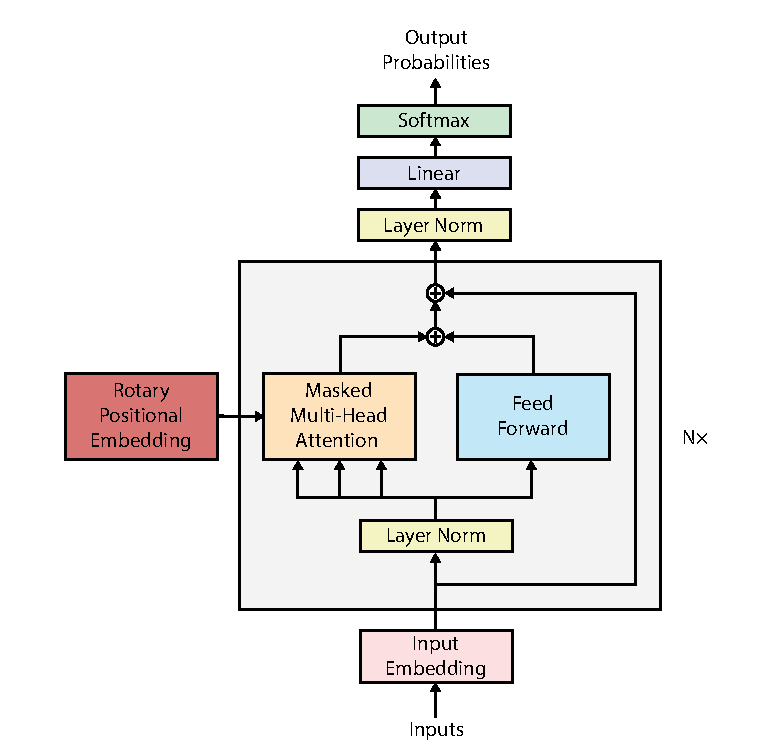
\includegraphics[width=0.5\columnwidth]{figures/gpt-j_architecture.pdf}
    \caption{Diagram of GPT-J model architecture.}
    \label{fig:gpt-j-architecture}
\end{figure}

\subsection{Step 2: Collect and label vulnerable code for vulnerability-tuning the model}
\label{sec:step2}
\subsubsection{Collect and label vulnerabilities data}
\label{sec:vulnerable-contracts}

Our labeled dataset is based on the dataset \footnote{\url{https://doi.org/10.5281/zenodo.7744053}} in \cite{Hu2023}, which contains manually labeled real-world vulnerable \acrshortpl{sc}. The dataset covers ten types of SC vulnerabilities. The dataset was acquired by running several SC code analysis tools to identify the vulnerabilities in 136,969 \acrshortpl{sc}. The authors then manually verified the resulting vulnerabilities to ensure they were vulnerable and exploitable. Although several other datasets, e.g., the dataset provided by \cite{solidifi} and  \cite{EmpiricalOnSmartBug}, are available, we believe the SCs in the dataset of \cite{Hu2023} are more reliable and contain more critical vulnerabilities because the focuses of \cite{Hu2023} is to eliminate false alarms of SC vulnerability detectors and focus on vulnerabilities that urgent to be fixed, i.e., the exploitable ones.

The dataset of \cite{Hu2023} does not provide the location of the vulnerabilities within a contract. We, therefore, reached out to the authors and got a copy of the SCs labeled by the different tools. Following \cite{Hu2023}, we only care about the contracts flagged as vulnerable by multiple tools. Since we need the actual line location of the vulnerabilities, we calculate the overlapping lines of the vulnerabilities within each SC. Different tools report slightly different results of the actual location of the vulnerabilities. To account for this, we allow some distance between the reported lines. We set this distance to \(\pm\) five lines. If multiple vulnerabilities occur within these ten lines, there will be duplications. We, therefore, filter the results so that each tool's reported vulnerability can only be used in one overlap combination while also selecting the combination that gives the minimum distance between the reported lines.

After calculating the overlapping vulnerabilities, we transfer these onto our inflated dataset, as described in \cref{sec:smart-contract-collection}. We then extract these contracts based on the contract addresses of the SCs in the dataset of \cite{Hu2023}. We get 609 vulnerable contracts containing 1,117  vulnerabilities. One vulnerable contract may contain several vulnerabilities.

\subsubsection{Using labeled vulnerable code for vulnerability-tuning}
\label{sec:labeling}

Starting from the fine-tuned model from step 1, we use the labeled vulnerable SC dataset for the model's future fine-tuning (called vulnerability-tuning from here). The goal is to train the model to generate vulnerability labels at the start of lines containing vulnerable code. Hence, the model learns to associate a particular label with a certain type of vulnerability. We prepend the vulnerable lines for each vulnerability in the dataset with the vulnerability label \(V_i\) corresponding to an abbreviation of its vulnerability type, e.g., IOU (meaning Integer Overflow or Underflow). Note that the labels will be inserted after whitespace indentation and before code statements. \Cref{lst:example-labeling} shows an example result after injecting an IOU label, marked in green.

\begin{lstlisting}[
    caption={Example of labeling a vulnerable line.},
    label=lst:example-labeling,
    language=Solidity,
    belowskip=0pt,
    escapechar=§]
function increaseLockTime(uint _seconds) public {
    §\lstbg{green!40}{<IOU>}§lockTime[msg.sender] += _seconds;
}
\end{lstlisting}


\subsection{Step 3: Vulnerability-constrained decoding}
To restrict the model during decoding (generation), we provide the model with a list of forbidden tokens (labels). Given a set of \(N\) vulnerability labels (tokens) \(V_i\), i.e., the abbreviations of different types of vulnerabilities, we manipulate the probability \(p\) for selecting any one of these during decoding, such that: \(p(x=V_i)=0\). 

\Cref{fig:greedy_search} shows an example of the vulnerability-constrained decoding method when using greedy search as the decoding strategy. Greedy search selects the token (word) with the highest probability as its next token: \(x_t = argmax_xP(x \mid x_{1:t-1}) \). Starting from the newline character to the left in the figure, a greedy search would normally have followed the solid red line. Assuming this path would lead to an IOU vulnerability, the model should have labeled this potential vulnerability with an \textless IOU\textgreater token (see \cref{sec:labeling}). If we apply the vulnerability-constrained decoding method, the decoding will avoid this path. It will select the second most probable path instead, following the stippled red line and avoiding the vulnerability altogether. Using a greedy search for decoding strategy is not optimal, as it will miss high-probability words disguised behind low-probability words. However, it is easy to understand and interpret the results. Our method is not limited to greedy decoding and is compatible with most other popular decoding strategies, such as Beam Search \cite{Freitag_2017}.

\begin{figure}[htp]
    \centering
    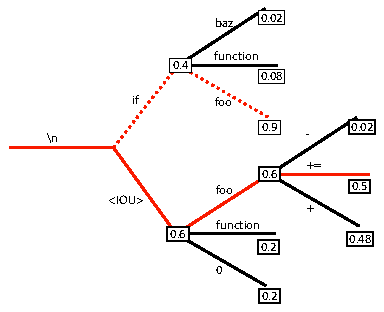
\includegraphics[width=0.5\columnwidth]{figures/greedy_search.pdf}
    \caption{Vulnerability-constrained decoding example using greedy search.}
    \label{fig:greedy_search}
\end{figure} 


\section{Implementation and Evaluation}
\label{chap:implementation-evaluation}

This section presents the detailed implementation of each step of our approach and the evaluation results.

\begin{comment}
    

    \begin{table}[htp]
\centering
\caption{Summary of results.}\label{tab:eval-summary}
\begin{threeparttable}
    %\newcolumntype{Y}{>{\centering\arraybackslash}X}
    %\newcolumntype{R}{>{\raggedright\arraybackslash}X}
    \def\arraystretch{1.5}
    \setlength\tabcolsep{2pt} % <--- important, (default 6pt)
    %\setlength{\LTleft}{-20cm plus -1fill}
    %\setlength{\LTright}{\LTleft}
    %\footnotesize
    %\begin{center}
    %\keepXColumns
    
    \begin{tabular}{p{1.5cm}ccp{1.25cm}p{1cm}p{2pt}p{1.25cm}p{1cm}}%RRRRR}
        \toprule
        \textbf{Model} & \textbf{ACC} & \textbf{PP} & \multicolumn{2}{c}{\textbf{BLEU score}} & & \multicolumn{2}{c}{\textbf{CrystalBLEU score}}\\\cline{4-5}\cline{7-8}
        & & & \textbf{WS} & \textbf{Solidity lexer} & & \textbf{WS} & \textbf{Solidity lexer} \\
        \midrule
        \textbf{Pre-trained} & 0.917 & 1.510 & 0.258 & 0.414 & & 0.188 & 0.291\\
        \textbf{Fine-tuned} &  &  & 0.557 & 0.557 & & 0.481 & 0.481 \\
        \textbf{Vulnerability-tuned} &  &  & 0.544 &  & &  & \\

       \bottomrule
    \end{tabular}
    \begin{tablenotes}
        %\item Some footnote here...
    \end{tablenotes}
    %\end{center}
\end{threeparttable}
\end{table}
\end{comment}


\subsection{Smart contract code generation}

\begin{table}[htp]
\centering
\caption{Summary of results.}\label{tab:eval-summary}
\begin{threeparttable}
    %\newcolumntype{Y}{>{\centering\arraybackslash}X}
    %\newcolumntype{R}{>{\raggedright\arraybackslash}X}
    \def\arraystretch{1.5}
    \setlength\tabcolsep{2pt} % <--- important, (default 6pt)
    %\setlength{\LTleft}{-20cm plus -1fill}
    %\setlength{\LTright}{\LTleft}
    %\footnotesize
    %\begin{center}
    %\keepXColumns
    
    \begin{tabular}{cccp{2pt}cc}%RRRRR}
        \toprule
        \textbf{Model} & \multicolumn{2}{c}{\textbf{BLEU score}} & & \multicolumn{2}{c}{\textbf{CrystalBLEU score}}\\\cline{2-3}\cline{5-6}
         & \textbf{Whitespace} & \textbf{Solidity lexer} & & \textbf{Whitespace} & \textbf{Solidity lexer} \\
        \midrule
        \textbf{Pre-trained} & 0.258 & 0.414 & & 0.188 & 0.291\\
        \textbf{Fine-tuned} & 0.557 & 0.557 & & 0.481 & 0.481 \\

       \bottomrule
    \end{tabular}
%    \begin{tablenotes}
%        %\item Some footnote here...
%    \end{tablenotes}
    %\end{center}
\end{threeparttable}
\end{table}

\subsubsection{Collected Unique Smart Contracts}
We retrieved 5,810,042 SC addresses from Google BigQuery by the 1st of April 2022. From these addresses, we successfully retrieved 2,217,692 verified SCs from Etherscan. The 2,217,692 SCs are inflated to 5,403,136 separate contract files. After filtering for uniqueness, 5,216,739 duplications are found, giving a duplication percentage of 96.56\%. The resulting Verified Smart Contracts dataset consists of 186,397 SCs. 

\subsubsection{Smart contract code generation model}
\label{sec:smart-contract-generation-model}

We used our collected SCs as the training dataset to fine-tune the pre-trained GPT-J-6B model for generating SC code. To ensure the validity of the model's performance, 80\% of the data were used for training, 10\% for validation, and 10\% for testing. No hyperparameter optimization was performed.

Before training, we randomly shuffled the dataset and fed a complete SC all at once to train the model. For running the training process, the \acrshort{clm} script \footnote{\url{https://github.com/huggingface/transformers/blob/v4.19.0/examples/pytorch/language-modeling/run_clm.py}} provided by HuggingFace was used. Due to the large size of the GPT-J-6B model, we used the deep learning optimization library DeepSpeed \cite{deepspeed} as a wrapper around the HuggingFace library. The training process runs for two epochs. At every five steps, the model is evaluated on 256 samples from the validation split of the SC dataset. Using \textbf{ten NVIDIA A100 40GB GPUs}, the training is completed after \textbf{seven days and four hours}. After completion of the training, the model is evaluated on the entire validation split, achieving an \acrfull{acc} of 0.917 and perplexity of 1.510.


\subsubsection{Evaluate the functionality of auto-completed SCs}
\label{sec:eval-quality-synthesis}
When evaluating code synthesizers, we hope the synthesized codes are similar to code that developers may input. Thus, we first measure \textbf{how well the model provides the desired functionality.} 

To answer this question, we used the original code developed by SC developers as the ground truth. We measured the similarity between the synthesized lines of code and the ground truth. The evaluation consists of three steps:
\begin{enumerate}
    \item We randomly selected SCs from the testing data.
    \item We split each of the selected SCs into two parts. The first part of each selected SC, which included code as the contexts and the comments, was used as the input to the model, while the second part (original code) was used as the ground truth.
    \item The generated lines of code were then compared to the ground truth to calculate their similarities.
\end{enumerate}

\Cref{lst:contract-parts} demonstrates how the different parts of a contract are used in the evaluation. Lines 1-11 are the code context, while lines 13-14 are the comments for the code synthesizer to generate code. The target codes (i.e., ground truth) are in lines 15-20. All consecutive lines of code are discarded. In \Cref{lst:contract-parts}, 
this would only be line 21. Since the model is auto-regressive, a custom stopping strategy based on matching braces is implemented for generating well-formed functions.


\begin{lstlisting}[
    caption={Different contract parts.},
    label=lst:contract-parts,
    language=Solidity,
    belowskip=0pt,
    escapechar=`]
// SPDX-License-Identifier: GPL-3.0
pragma solidity >= 0.7.0;

contract Coin {
    // Sends an amount of newly created coins to an address
    // Can only be called by the contract creator
    function mint(address receiver, uint amount) public {
        require(msg.sender == minter);
        require(amount < 1e60);
        balances[receiver] += amount;
    }
    
\end{lstlisting}
\begin{lstlisting}[
    frame=bottomline,
    firstnumber=13,
    aboveskip=0pt,
    language=Solidity,
    escapechar=`
    ]
    // Sends an amount of existing coins
    // from any caller to an address
\end{lstlisting}
\begin{lstlisting}[
    frame=bottomline,
    firstnumber=15,
    aboveskip=0pt,
    language=Solidity,
    escapechar=`
    ]
    function send(address receiver, uint amount) public {
        require(amount <= balances[msg.sender], "Insufficient balance.");
        balances[msg.sender] -= amount;
        balances[receiver] += amount;
        emit Sent(msg.sender, receiver, amount);
    }
\end{lstlisting}
\begin{lstlisting}[
    frame=bottomline,
    firstnumber=21,
    aboveskip=0pt,
    language=Solidity,
    escapechar=`
    ]
}
\end{lstlisting}

The BLEU score compares the generated code to ground truth. BLEU is a commonly used evaluation metric in code synthesis \cite{ren2020codebleu}. However, as BLEU was originally designed for evaluating natural language, it has shortcomings when applied to evaluate code synthesizers because it neglects important syntactic and semantic aspects of codes \cite{ren2020codebleu}. Due to this limitation, adaptations, e.g., CodeBLEU by \cite{ren2020codebleu}, have emerged, incorporating Abstract Syntex Tree (AST) and data-flow analysis. However, we could not find a readily available implementation of CodeBLEU, especially for SC. CrystalBLEU \cite{CrystalBLEU} is a recently (in 2022) proposed metric to compare code similarity. Thus, we decide to measure the code similarity using both BLEU and CrystalBLEU. To use BLEU or CrystalBLEU to measure code similarity, we must configure the tokenization approach. We can for example tokenize using whitespace or a lexer for the programming language, e.g., Solidity.

We randomly selected 10,000 SC samples from the test split of the Verified Smart Contract Code Comments dataset. Each drawn sample contains function ``code, comment'' pairs, and the complete contract code. The contract code is cut at the end of the sampled function comment and fed into the model as input to generate code. The BLEU and CrystalBLEU scores are calculated by comparing the generated code against the ground truth.  We performed the evaluation procedure for the pre-trained and fine-tuned models. The BLEU results using whitespace as the splitter are shown in Figures \ref{fig:performance-code-context_pretrained} and \ref{fig:performance-code-context_finetuned}. On average, the pre-trained model's BLEU is only 0.258, and the fine-tuned transformer achieves a BLEU score of 0.557. This is over a 100\% improvement from the pre-trained model. To calculate CrystalBLEU, we need to configure some parameters: K (trivially shared n-grams samples) and maxN (n-grams from 1 to maxN). This study configures their values as 500 and four, respectively. The CrystalBLEU results using whitespace as the splitter are 0.188 and 0.481 for the pre-trained and the fine-tuned models, respectively. The results also show over a 100\% improvement from the pre-trained model. By using a lexer for the Solidity programming language to tokenize, the BLEU score increased from 0.414 to 0.557 after transformer fine-tuning, and the CrystalBLEU increased from 0.291 to 0.481. The results are summarized in Table \ref{tab:eval-summary}. 


\begin{figure}[htp]
    \centering
    %% Creator: Matplotlib, PGF backend
%%
%% To include the figure in your LaTeX document, write
%%   \input{<filename>.pgf}
%%
%% Make sure the required packages are loaded in your preamble
%%   \usepackage{pgf}
%%
%% Also ensure that all the required font packages are loaded; for instance,
%% the lmodern package is sometimes necessary when using math font.
%%   \usepackage{lmodern}
%%
%% Figures using additional raster images can only be included by \input if
%% they are in the same directory as the main LaTeX file. For loading figures
%% from other directories you can use the `import` package
%%   \usepackage{import}
%%
%% and then include the figures with
%%   \import{<path to file>}{<filename>.pgf}
%%
%% Matplotlib used the following preamble
%%
\begingroup%
\makeatletter%
\begin{pgfpicture}%
\pgfpathrectangle{\pgfpointorigin}{\pgfqpoint{3.331375in}{2.732666in}}%
\pgfusepath{use as bounding box, clip}%
\begin{pgfscope}%
\pgfsetbuttcap%
\pgfsetmiterjoin%
\pgfsetlinewidth{0.000000pt}%
\definecolor{currentstroke}{rgb}{1.000000,1.000000,1.000000}%
\pgfsetstrokecolor{currentstroke}%
\pgfsetstrokeopacity{0.000000}%
\pgfsetdash{}{0pt}%
\pgfpathmoveto{\pgfqpoint{0.000000in}{0.000000in}}%
\pgfpathlineto{\pgfqpoint{3.331375in}{0.000000in}}%
\pgfpathlineto{\pgfqpoint{3.331375in}{2.732666in}}%
\pgfpathlineto{\pgfqpoint{0.000000in}{2.732666in}}%
\pgfpathlineto{\pgfqpoint{0.000000in}{0.000000in}}%
\pgfpathclose%
\pgfusepath{}%
\end{pgfscope}%
\begin{pgfscope}%
\pgfsetbuttcap%
\pgfsetmiterjoin%
\definecolor{currentfill}{rgb}{1.000000,1.000000,1.000000}%
\pgfsetfillcolor{currentfill}%
\pgfsetlinewidth{0.000000pt}%
\definecolor{currentstroke}{rgb}{0.000000,0.000000,0.000000}%
\pgfsetstrokecolor{currentstroke}%
\pgfsetstrokeopacity{0.000000}%
\pgfsetdash{}{0pt}%
\pgfpathmoveto{\pgfqpoint{0.620832in}{0.475000in}}%
\pgfpathlineto{\pgfqpoint{3.231375in}{0.475000in}}%
\pgfpathlineto{\pgfqpoint{3.231375in}{2.443719in}}%
\pgfpathlineto{\pgfqpoint{0.620832in}{2.443719in}}%
\pgfpathlineto{\pgfqpoint{0.620832in}{0.475000in}}%
\pgfpathclose%
\pgfusepath{fill}%
\end{pgfscope}%
\begin{pgfscope}%
\pgfpathrectangle{\pgfqpoint{0.620832in}{0.475000in}}{\pgfqpoint{2.610543in}{1.968719in}}%
\pgfusepath{clip}%
\pgfsetbuttcap%
\pgfsetmiterjoin%
\definecolor{currentfill}{rgb}{0.121569,0.466667,0.705882}%
\pgfsetfillcolor{currentfill}%
\pgfsetlinewidth{0.000000pt}%
\definecolor{currentstroke}{rgb}{0.000000,0.000000,0.000000}%
\pgfsetstrokecolor{currentstroke}%
\pgfsetstrokeopacity{0.000000}%
\pgfsetdash{}{0pt}%
\pgfpathmoveto{\pgfqpoint{0.739493in}{0.475000in}}%
\pgfpathlineto{\pgfqpoint{0.858154in}{0.475000in}}%
\pgfpathlineto{\pgfqpoint{0.858154in}{2.378970in}}%
\pgfpathlineto{\pgfqpoint{0.739493in}{2.378970in}}%
\pgfpathlineto{\pgfqpoint{0.739493in}{0.475000in}}%
\pgfpathclose%
\pgfusepath{fill}%
\end{pgfscope}%
\begin{pgfscope}%
\pgfpathrectangle{\pgfqpoint{0.620832in}{0.475000in}}{\pgfqpoint{2.610543in}{1.968719in}}%
\pgfusepath{clip}%
\pgfsetbuttcap%
\pgfsetmiterjoin%
\definecolor{currentfill}{rgb}{0.121569,0.466667,0.705882}%
\pgfsetfillcolor{currentfill}%
\pgfsetlinewidth{0.000000pt}%
\definecolor{currentstroke}{rgb}{0.000000,0.000000,0.000000}%
\pgfsetstrokecolor{currentstroke}%
\pgfsetstrokeopacity{0.000000}%
\pgfsetdash{}{0pt}%
\pgfpathmoveto{\pgfqpoint{0.858154in}{0.475000in}}%
\pgfpathlineto{\pgfqpoint{0.976815in}{0.475000in}}%
\pgfpathlineto{\pgfqpoint{0.976815in}{0.726559in}}%
\pgfpathlineto{\pgfqpoint{0.858154in}{0.726559in}}%
\pgfpathlineto{\pgfqpoint{0.858154in}{0.475000in}}%
\pgfpathclose%
\pgfusepath{fill}%
\end{pgfscope}%
\begin{pgfscope}%
\pgfpathrectangle{\pgfqpoint{0.620832in}{0.475000in}}{\pgfqpoint{2.610543in}{1.968719in}}%
\pgfusepath{clip}%
\pgfsetbuttcap%
\pgfsetmiterjoin%
\definecolor{currentfill}{rgb}{0.121569,0.466667,0.705882}%
\pgfsetfillcolor{currentfill}%
\pgfsetlinewidth{0.000000pt}%
\definecolor{currentstroke}{rgb}{0.000000,0.000000,0.000000}%
\pgfsetstrokecolor{currentstroke}%
\pgfsetstrokeopacity{0.000000}%
\pgfsetdash{}{0pt}%
\pgfpathmoveto{\pgfqpoint{0.976815in}{0.475000in}}%
\pgfpathlineto{\pgfqpoint{1.095476in}{0.475000in}}%
\pgfpathlineto{\pgfqpoint{1.095476in}{0.716496in}}%
\pgfpathlineto{\pgfqpoint{0.976815in}{0.716496in}}%
\pgfpathlineto{\pgfqpoint{0.976815in}{0.475000in}}%
\pgfpathclose%
\pgfusepath{fill}%
\end{pgfscope}%
\begin{pgfscope}%
\pgfpathrectangle{\pgfqpoint{0.620832in}{0.475000in}}{\pgfqpoint{2.610543in}{1.968719in}}%
\pgfusepath{clip}%
\pgfsetbuttcap%
\pgfsetmiterjoin%
\definecolor{currentfill}{rgb}{0.121569,0.466667,0.705882}%
\pgfsetfillcolor{currentfill}%
\pgfsetlinewidth{0.000000pt}%
\definecolor{currentstroke}{rgb}{0.000000,0.000000,0.000000}%
\pgfsetstrokecolor{currentstroke}%
\pgfsetstrokeopacity{0.000000}%
\pgfsetdash{}{0pt}%
\pgfpathmoveto{\pgfqpoint{1.095476in}{0.475000in}}%
\pgfpathlineto{\pgfqpoint{1.214137in}{0.475000in}}%
\pgfpathlineto{\pgfqpoint{1.214137in}{0.660497in}}%
\pgfpathlineto{\pgfqpoint{1.095476in}{0.660497in}}%
\pgfpathlineto{\pgfqpoint{1.095476in}{0.475000in}}%
\pgfpathclose%
\pgfusepath{fill}%
\end{pgfscope}%
\begin{pgfscope}%
\pgfpathrectangle{\pgfqpoint{0.620832in}{0.475000in}}{\pgfqpoint{2.610543in}{1.968719in}}%
\pgfusepath{clip}%
\pgfsetbuttcap%
\pgfsetmiterjoin%
\definecolor{currentfill}{rgb}{0.121569,0.466667,0.705882}%
\pgfsetfillcolor{currentfill}%
\pgfsetlinewidth{0.000000pt}%
\definecolor{currentstroke}{rgb}{0.000000,0.000000,0.000000}%
\pgfsetstrokecolor{currentstroke}%
\pgfsetstrokeopacity{0.000000}%
\pgfsetdash{}{0pt}%
\pgfpathmoveto{\pgfqpoint{1.214137in}{0.475000in}}%
\pgfpathlineto{\pgfqpoint{1.332798in}{0.475000in}}%
\pgfpathlineto{\pgfqpoint{1.332798in}{0.623310in}}%
\pgfpathlineto{\pgfqpoint{1.214137in}{0.623310in}}%
\pgfpathlineto{\pgfqpoint{1.214137in}{0.475000in}}%
\pgfpathclose%
\pgfusepath{fill}%
\end{pgfscope}%
\begin{pgfscope}%
\pgfpathrectangle{\pgfqpoint{0.620832in}{0.475000in}}{\pgfqpoint{2.610543in}{1.968719in}}%
\pgfusepath{clip}%
\pgfsetbuttcap%
\pgfsetmiterjoin%
\definecolor{currentfill}{rgb}{0.121569,0.466667,0.705882}%
\pgfsetfillcolor{currentfill}%
\pgfsetlinewidth{0.000000pt}%
\definecolor{currentstroke}{rgb}{0.000000,0.000000,0.000000}%
\pgfsetstrokecolor{currentstroke}%
\pgfsetstrokeopacity{0.000000}%
\pgfsetdash{}{0pt}%
\pgfpathmoveto{\pgfqpoint{1.332798in}{0.475000in}}%
\pgfpathlineto{\pgfqpoint{1.451459in}{0.475000in}}%
\pgfpathlineto{\pgfqpoint{1.451459in}{0.620248in}}%
\pgfpathlineto{\pgfqpoint{1.332798in}{0.620248in}}%
\pgfpathlineto{\pgfqpoint{1.332798in}{0.475000in}}%
\pgfpathclose%
\pgfusepath{fill}%
\end{pgfscope}%
\begin{pgfscope}%
\pgfpathrectangle{\pgfqpoint{0.620832in}{0.475000in}}{\pgfqpoint{2.610543in}{1.968719in}}%
\pgfusepath{clip}%
\pgfsetbuttcap%
\pgfsetmiterjoin%
\definecolor{currentfill}{rgb}{0.121569,0.466667,0.705882}%
\pgfsetfillcolor{currentfill}%
\pgfsetlinewidth{0.000000pt}%
\definecolor{currentstroke}{rgb}{0.000000,0.000000,0.000000}%
\pgfsetstrokecolor{currentstroke}%
\pgfsetstrokeopacity{0.000000}%
\pgfsetdash{}{0pt}%
\pgfpathmoveto{\pgfqpoint{1.451459in}{0.475000in}}%
\pgfpathlineto{\pgfqpoint{1.570120in}{0.475000in}}%
\pgfpathlineto{\pgfqpoint{1.570120in}{0.631185in}}%
\pgfpathlineto{\pgfqpoint{1.451459in}{0.631185in}}%
\pgfpathlineto{\pgfqpoint{1.451459in}{0.475000in}}%
\pgfpathclose%
\pgfusepath{fill}%
\end{pgfscope}%
\begin{pgfscope}%
\pgfpathrectangle{\pgfqpoint{0.620832in}{0.475000in}}{\pgfqpoint{2.610543in}{1.968719in}}%
\pgfusepath{clip}%
\pgfsetbuttcap%
\pgfsetmiterjoin%
\definecolor{currentfill}{rgb}{0.121569,0.466667,0.705882}%
\pgfsetfillcolor{currentfill}%
\pgfsetlinewidth{0.000000pt}%
\definecolor{currentstroke}{rgb}{0.000000,0.000000,0.000000}%
\pgfsetstrokecolor{currentstroke}%
\pgfsetstrokeopacity{0.000000}%
\pgfsetdash{}{0pt}%
\pgfpathmoveto{\pgfqpoint{1.570120in}{0.475000in}}%
\pgfpathlineto{\pgfqpoint{1.688781in}{0.475000in}}%
\pgfpathlineto{\pgfqpoint{1.688781in}{0.557686in}}%
\pgfpathlineto{\pgfqpoint{1.570120in}{0.557686in}}%
\pgfpathlineto{\pgfqpoint{1.570120in}{0.475000in}}%
\pgfpathclose%
\pgfusepath{fill}%
\end{pgfscope}%
\begin{pgfscope}%
\pgfpathrectangle{\pgfqpoint{0.620832in}{0.475000in}}{\pgfqpoint{2.610543in}{1.968719in}}%
\pgfusepath{clip}%
\pgfsetbuttcap%
\pgfsetmiterjoin%
\definecolor{currentfill}{rgb}{0.121569,0.466667,0.705882}%
\pgfsetfillcolor{currentfill}%
\pgfsetlinewidth{0.000000pt}%
\definecolor{currentstroke}{rgb}{0.000000,0.000000,0.000000}%
\pgfsetstrokecolor{currentstroke}%
\pgfsetstrokeopacity{0.000000}%
\pgfsetdash{}{0pt}%
\pgfpathmoveto{\pgfqpoint{1.688781in}{0.475000in}}%
\pgfpathlineto{\pgfqpoint{1.807442in}{0.475000in}}%
\pgfpathlineto{\pgfqpoint{1.807442in}{0.630748in}}%
\pgfpathlineto{\pgfqpoint{1.688781in}{0.630748in}}%
\pgfpathlineto{\pgfqpoint{1.688781in}{0.475000in}}%
\pgfpathclose%
\pgfusepath{fill}%
\end{pgfscope}%
\begin{pgfscope}%
\pgfpathrectangle{\pgfqpoint{0.620832in}{0.475000in}}{\pgfqpoint{2.610543in}{1.968719in}}%
\pgfusepath{clip}%
\pgfsetbuttcap%
\pgfsetmiterjoin%
\definecolor{currentfill}{rgb}{0.121569,0.466667,0.705882}%
\pgfsetfillcolor{currentfill}%
\pgfsetlinewidth{0.000000pt}%
\definecolor{currentstroke}{rgb}{0.000000,0.000000,0.000000}%
\pgfsetstrokecolor{currentstroke}%
\pgfsetstrokeopacity{0.000000}%
\pgfsetdash{}{0pt}%
\pgfpathmoveto{\pgfqpoint{1.807442in}{0.475000in}}%
\pgfpathlineto{\pgfqpoint{1.926103in}{0.475000in}}%
\pgfpathlineto{\pgfqpoint{1.926103in}{0.548499in}}%
\pgfpathlineto{\pgfqpoint{1.807442in}{0.548499in}}%
\pgfpathlineto{\pgfqpoint{1.807442in}{0.475000in}}%
\pgfpathclose%
\pgfusepath{fill}%
\end{pgfscope}%
\begin{pgfscope}%
\pgfpathrectangle{\pgfqpoint{0.620832in}{0.475000in}}{\pgfqpoint{2.610543in}{1.968719in}}%
\pgfusepath{clip}%
\pgfsetbuttcap%
\pgfsetmiterjoin%
\definecolor{currentfill}{rgb}{0.121569,0.466667,0.705882}%
\pgfsetfillcolor{currentfill}%
\pgfsetlinewidth{0.000000pt}%
\definecolor{currentstroke}{rgb}{0.000000,0.000000,0.000000}%
\pgfsetstrokecolor{currentstroke}%
\pgfsetstrokeopacity{0.000000}%
\pgfsetdash{}{0pt}%
\pgfpathmoveto{\pgfqpoint{1.926103in}{0.475000in}}%
\pgfpathlineto{\pgfqpoint{2.044764in}{0.475000in}}%
\pgfpathlineto{\pgfqpoint{2.044764in}{0.590936in}}%
\pgfpathlineto{\pgfqpoint{1.926103in}{0.590936in}}%
\pgfpathlineto{\pgfqpoint{1.926103in}{0.475000in}}%
\pgfpathclose%
\pgfusepath{fill}%
\end{pgfscope}%
\begin{pgfscope}%
\pgfpathrectangle{\pgfqpoint{0.620832in}{0.475000in}}{\pgfqpoint{2.610543in}{1.968719in}}%
\pgfusepath{clip}%
\pgfsetbuttcap%
\pgfsetmiterjoin%
\definecolor{currentfill}{rgb}{0.121569,0.466667,0.705882}%
\pgfsetfillcolor{currentfill}%
\pgfsetlinewidth{0.000000pt}%
\definecolor{currentstroke}{rgb}{0.000000,0.000000,0.000000}%
\pgfsetstrokecolor{currentstroke}%
\pgfsetstrokeopacity{0.000000}%
\pgfsetdash{}{0pt}%
\pgfpathmoveto{\pgfqpoint{2.044764in}{0.475000in}}%
\pgfpathlineto{\pgfqpoint{2.163425in}{0.475000in}}%
\pgfpathlineto{\pgfqpoint{2.163425in}{0.556374in}}%
\pgfpathlineto{\pgfqpoint{2.044764in}{0.556374in}}%
\pgfpathlineto{\pgfqpoint{2.044764in}{0.475000in}}%
\pgfpathclose%
\pgfusepath{fill}%
\end{pgfscope}%
\begin{pgfscope}%
\pgfpathrectangle{\pgfqpoint{0.620832in}{0.475000in}}{\pgfqpoint{2.610543in}{1.968719in}}%
\pgfusepath{clip}%
\pgfsetbuttcap%
\pgfsetmiterjoin%
\definecolor{currentfill}{rgb}{0.121569,0.466667,0.705882}%
\pgfsetfillcolor{currentfill}%
\pgfsetlinewidth{0.000000pt}%
\definecolor{currentstroke}{rgb}{0.000000,0.000000,0.000000}%
\pgfsetstrokecolor{currentstroke}%
\pgfsetstrokeopacity{0.000000}%
\pgfsetdash{}{0pt}%
\pgfpathmoveto{\pgfqpoint{2.163425in}{0.475000in}}%
\pgfpathlineto{\pgfqpoint{2.282087in}{0.475000in}}%
\pgfpathlineto{\pgfqpoint{2.282087in}{0.573873in}}%
\pgfpathlineto{\pgfqpoint{2.163425in}{0.573873in}}%
\pgfpathlineto{\pgfqpoint{2.163425in}{0.475000in}}%
\pgfpathclose%
\pgfusepath{fill}%
\end{pgfscope}%
\begin{pgfscope}%
\pgfpathrectangle{\pgfqpoint{0.620832in}{0.475000in}}{\pgfqpoint{2.610543in}{1.968719in}}%
\pgfusepath{clip}%
\pgfsetbuttcap%
\pgfsetmiterjoin%
\definecolor{currentfill}{rgb}{0.121569,0.466667,0.705882}%
\pgfsetfillcolor{currentfill}%
\pgfsetlinewidth{0.000000pt}%
\definecolor{currentstroke}{rgb}{0.000000,0.000000,0.000000}%
\pgfsetstrokecolor{currentstroke}%
\pgfsetstrokeopacity{0.000000}%
\pgfsetdash{}{0pt}%
\pgfpathmoveto{\pgfqpoint{2.282087in}{0.475000in}}%
\pgfpathlineto{\pgfqpoint{2.400748in}{0.475000in}}%
\pgfpathlineto{\pgfqpoint{2.400748in}{0.538437in}}%
\pgfpathlineto{\pgfqpoint{2.282087in}{0.538437in}}%
\pgfpathlineto{\pgfqpoint{2.282087in}{0.475000in}}%
\pgfpathclose%
\pgfusepath{fill}%
\end{pgfscope}%
\begin{pgfscope}%
\pgfpathrectangle{\pgfqpoint{0.620832in}{0.475000in}}{\pgfqpoint{2.610543in}{1.968719in}}%
\pgfusepath{clip}%
\pgfsetbuttcap%
\pgfsetmiterjoin%
\definecolor{currentfill}{rgb}{0.121569,0.466667,0.705882}%
\pgfsetfillcolor{currentfill}%
\pgfsetlinewidth{0.000000pt}%
\definecolor{currentstroke}{rgb}{0.000000,0.000000,0.000000}%
\pgfsetstrokecolor{currentstroke}%
\pgfsetstrokeopacity{0.000000}%
\pgfsetdash{}{0pt}%
\pgfpathmoveto{\pgfqpoint{2.400748in}{0.475000in}}%
\pgfpathlineto{\pgfqpoint{2.519409in}{0.475000in}}%
\pgfpathlineto{\pgfqpoint{2.519409in}{0.538874in}}%
\pgfpathlineto{\pgfqpoint{2.400748in}{0.538874in}}%
\pgfpathlineto{\pgfqpoint{2.400748in}{0.475000in}}%
\pgfpathclose%
\pgfusepath{fill}%
\end{pgfscope}%
\begin{pgfscope}%
\pgfpathrectangle{\pgfqpoint{0.620832in}{0.475000in}}{\pgfqpoint{2.610543in}{1.968719in}}%
\pgfusepath{clip}%
\pgfsetbuttcap%
\pgfsetmiterjoin%
\definecolor{currentfill}{rgb}{0.121569,0.466667,0.705882}%
\pgfsetfillcolor{currentfill}%
\pgfsetlinewidth{0.000000pt}%
\definecolor{currentstroke}{rgb}{0.000000,0.000000,0.000000}%
\pgfsetstrokecolor{currentstroke}%
\pgfsetstrokeopacity{0.000000}%
\pgfsetdash{}{0pt}%
\pgfpathmoveto{\pgfqpoint{2.519409in}{0.475000in}}%
\pgfpathlineto{\pgfqpoint{2.638070in}{0.475000in}}%
\pgfpathlineto{\pgfqpoint{2.638070in}{0.546749in}}%
\pgfpathlineto{\pgfqpoint{2.519409in}{0.546749in}}%
\pgfpathlineto{\pgfqpoint{2.519409in}{0.475000in}}%
\pgfpathclose%
\pgfusepath{fill}%
\end{pgfscope}%
\begin{pgfscope}%
\pgfpathrectangle{\pgfqpoint{0.620832in}{0.475000in}}{\pgfqpoint{2.610543in}{1.968719in}}%
\pgfusepath{clip}%
\pgfsetbuttcap%
\pgfsetmiterjoin%
\definecolor{currentfill}{rgb}{0.121569,0.466667,0.705882}%
\pgfsetfillcolor{currentfill}%
\pgfsetlinewidth{0.000000pt}%
\definecolor{currentstroke}{rgb}{0.000000,0.000000,0.000000}%
\pgfsetstrokecolor{currentstroke}%
\pgfsetstrokeopacity{0.000000}%
\pgfsetdash{}{0pt}%
\pgfpathmoveto{\pgfqpoint{2.638070in}{0.475000in}}%
\pgfpathlineto{\pgfqpoint{2.756731in}{0.475000in}}%
\pgfpathlineto{\pgfqpoint{2.756731in}{0.668809in}}%
\pgfpathlineto{\pgfqpoint{2.638070in}{0.668809in}}%
\pgfpathlineto{\pgfqpoint{2.638070in}{0.475000in}}%
\pgfpathclose%
\pgfusepath{fill}%
\end{pgfscope}%
\begin{pgfscope}%
\pgfpathrectangle{\pgfqpoint{0.620832in}{0.475000in}}{\pgfqpoint{2.610543in}{1.968719in}}%
\pgfusepath{clip}%
\pgfsetbuttcap%
\pgfsetmiterjoin%
\definecolor{currentfill}{rgb}{0.121569,0.466667,0.705882}%
\pgfsetfillcolor{currentfill}%
\pgfsetlinewidth{0.000000pt}%
\definecolor{currentstroke}{rgb}{0.000000,0.000000,0.000000}%
\pgfsetstrokecolor{currentstroke}%
\pgfsetstrokeopacity{0.000000}%
\pgfsetdash{}{0pt}%
\pgfpathmoveto{\pgfqpoint{2.756731in}{0.475000in}}%
\pgfpathlineto{\pgfqpoint{2.875392in}{0.475000in}}%
\pgfpathlineto{\pgfqpoint{2.875392in}{0.625498in}}%
\pgfpathlineto{\pgfqpoint{2.756731in}{0.625498in}}%
\pgfpathlineto{\pgfqpoint{2.756731in}{0.475000in}}%
\pgfpathclose%
\pgfusepath{fill}%
\end{pgfscope}%
\begin{pgfscope}%
\pgfpathrectangle{\pgfqpoint{0.620832in}{0.475000in}}{\pgfqpoint{2.610543in}{1.968719in}}%
\pgfusepath{clip}%
\pgfsetbuttcap%
\pgfsetmiterjoin%
\definecolor{currentfill}{rgb}{0.121569,0.466667,0.705882}%
\pgfsetfillcolor{currentfill}%
\pgfsetlinewidth{0.000000pt}%
\definecolor{currentstroke}{rgb}{0.000000,0.000000,0.000000}%
\pgfsetstrokecolor{currentstroke}%
\pgfsetstrokeopacity{0.000000}%
\pgfsetdash{}{0pt}%
\pgfpathmoveto{\pgfqpoint{2.875392in}{0.475000in}}%
\pgfpathlineto{\pgfqpoint{2.994053in}{0.475000in}}%
\pgfpathlineto{\pgfqpoint{2.994053in}{0.599248in}}%
\pgfpathlineto{\pgfqpoint{2.875392in}{0.599248in}}%
\pgfpathlineto{\pgfqpoint{2.875392in}{0.475000in}}%
\pgfpathclose%
\pgfusepath{fill}%
\end{pgfscope}%
\begin{pgfscope}%
\pgfpathrectangle{\pgfqpoint{0.620832in}{0.475000in}}{\pgfqpoint{2.610543in}{1.968719in}}%
\pgfusepath{clip}%
\pgfsetbuttcap%
\pgfsetmiterjoin%
\definecolor{currentfill}{rgb}{0.121569,0.466667,0.705882}%
\pgfsetfillcolor{currentfill}%
\pgfsetlinewidth{0.000000pt}%
\definecolor{currentstroke}{rgb}{0.000000,0.000000,0.000000}%
\pgfsetstrokecolor{currentstroke}%
\pgfsetstrokeopacity{0.000000}%
\pgfsetdash{}{0pt}%
\pgfpathmoveto{\pgfqpoint{2.994053in}{0.475000in}}%
\pgfpathlineto{\pgfqpoint{3.112714in}{0.475000in}}%
\pgfpathlineto{\pgfqpoint{3.112714in}{0.541936in}}%
\pgfpathlineto{\pgfqpoint{2.994053in}{0.541936in}}%
\pgfpathlineto{\pgfqpoint{2.994053in}{0.475000in}}%
\pgfpathclose%
\pgfusepath{fill}%
\end{pgfscope}%
\begin{pgfscope}%
\pgfsetbuttcap%
\pgfsetroundjoin%
\definecolor{currentfill}{rgb}{0.000000,0.000000,0.000000}%
\pgfsetfillcolor{currentfill}%
\pgfsetlinewidth{0.803000pt}%
\definecolor{currentstroke}{rgb}{0.000000,0.000000,0.000000}%
\pgfsetstrokecolor{currentstroke}%
\pgfsetdash{}{0pt}%
\pgfsys@defobject{currentmarker}{\pgfqpoint{0.000000in}{-0.048611in}}{\pgfqpoint{0.000000in}{0.000000in}}{%
\pgfpathmoveto{\pgfqpoint{0.000000in}{0.000000in}}%
\pgfpathlineto{\pgfqpoint{0.000000in}{-0.048611in}}%
\pgfusepath{stroke,fill}%
}%
\begin{pgfscope}%
\pgfsys@transformshift{0.739493in}{0.475000in}%
\pgfsys@useobject{currentmarker}{}%
\end{pgfscope}%
\end{pgfscope}%
\begin{pgfscope}%
\definecolor{textcolor}{rgb}{0.000000,0.000000,0.000000}%
\pgfsetstrokecolor{textcolor}%
\pgfsetfillcolor{textcolor}%
\pgftext[x=0.739493in,y=0.377778in,,top]{\color{textcolor}\rmfamily\fontsize{9.000000}{10.800000}\selectfont \(\displaystyle {0.0}\)}%
\end{pgfscope}%
\begin{pgfscope}%
\pgfsetbuttcap%
\pgfsetroundjoin%
\definecolor{currentfill}{rgb}{0.000000,0.000000,0.000000}%
\pgfsetfillcolor{currentfill}%
\pgfsetlinewidth{0.803000pt}%
\definecolor{currentstroke}{rgb}{0.000000,0.000000,0.000000}%
\pgfsetstrokecolor{currentstroke}%
\pgfsetdash{}{0pt}%
\pgfsys@defobject{currentmarker}{\pgfqpoint{0.000000in}{-0.048611in}}{\pgfqpoint{0.000000in}{0.000000in}}{%
\pgfpathmoveto{\pgfqpoint{0.000000in}{0.000000in}}%
\pgfpathlineto{\pgfqpoint{0.000000in}{-0.048611in}}%
\pgfusepath{stroke,fill}%
}%
\begin{pgfscope}%
\pgfsys@transformshift{1.214137in}{0.475000in}%
\pgfsys@useobject{currentmarker}{}%
\end{pgfscope}%
\end{pgfscope}%
\begin{pgfscope}%
\definecolor{textcolor}{rgb}{0.000000,0.000000,0.000000}%
\pgfsetstrokecolor{textcolor}%
\pgfsetfillcolor{textcolor}%
\pgftext[x=1.214137in,y=0.377778in,,top]{\color{textcolor}\rmfamily\fontsize{9.000000}{10.800000}\selectfont \(\displaystyle {0.2}\)}%
\end{pgfscope}%
\begin{pgfscope}%
\pgfsetbuttcap%
\pgfsetroundjoin%
\definecolor{currentfill}{rgb}{0.000000,0.000000,0.000000}%
\pgfsetfillcolor{currentfill}%
\pgfsetlinewidth{0.803000pt}%
\definecolor{currentstroke}{rgb}{0.000000,0.000000,0.000000}%
\pgfsetstrokecolor{currentstroke}%
\pgfsetdash{}{0pt}%
\pgfsys@defobject{currentmarker}{\pgfqpoint{0.000000in}{-0.048611in}}{\pgfqpoint{0.000000in}{0.000000in}}{%
\pgfpathmoveto{\pgfqpoint{0.000000in}{0.000000in}}%
\pgfpathlineto{\pgfqpoint{0.000000in}{-0.048611in}}%
\pgfusepath{stroke,fill}%
}%
\begin{pgfscope}%
\pgfsys@transformshift{1.688781in}{0.475000in}%
\pgfsys@useobject{currentmarker}{}%
\end{pgfscope}%
\end{pgfscope}%
\begin{pgfscope}%
\definecolor{textcolor}{rgb}{0.000000,0.000000,0.000000}%
\pgfsetstrokecolor{textcolor}%
\pgfsetfillcolor{textcolor}%
\pgftext[x=1.688781in,y=0.377778in,,top]{\color{textcolor}\rmfamily\fontsize{9.000000}{10.800000}\selectfont \(\displaystyle {0.4}\)}%
\end{pgfscope}%
\begin{pgfscope}%
\pgfsetbuttcap%
\pgfsetroundjoin%
\definecolor{currentfill}{rgb}{0.000000,0.000000,0.000000}%
\pgfsetfillcolor{currentfill}%
\pgfsetlinewidth{0.803000pt}%
\definecolor{currentstroke}{rgb}{0.000000,0.000000,0.000000}%
\pgfsetstrokecolor{currentstroke}%
\pgfsetdash{}{0pt}%
\pgfsys@defobject{currentmarker}{\pgfqpoint{0.000000in}{-0.048611in}}{\pgfqpoint{0.000000in}{0.000000in}}{%
\pgfpathmoveto{\pgfqpoint{0.000000in}{0.000000in}}%
\pgfpathlineto{\pgfqpoint{0.000000in}{-0.048611in}}%
\pgfusepath{stroke,fill}%
}%
\begin{pgfscope}%
\pgfsys@transformshift{2.163425in}{0.475000in}%
\pgfsys@useobject{currentmarker}{}%
\end{pgfscope}%
\end{pgfscope}%
\begin{pgfscope}%
\definecolor{textcolor}{rgb}{0.000000,0.000000,0.000000}%
\pgfsetstrokecolor{textcolor}%
\pgfsetfillcolor{textcolor}%
\pgftext[x=2.163425in,y=0.377778in,,top]{\color{textcolor}\rmfamily\fontsize{9.000000}{10.800000}\selectfont \(\displaystyle {0.6}\)}%
\end{pgfscope}%
\begin{pgfscope}%
\pgfsetbuttcap%
\pgfsetroundjoin%
\definecolor{currentfill}{rgb}{0.000000,0.000000,0.000000}%
\pgfsetfillcolor{currentfill}%
\pgfsetlinewidth{0.803000pt}%
\definecolor{currentstroke}{rgb}{0.000000,0.000000,0.000000}%
\pgfsetstrokecolor{currentstroke}%
\pgfsetdash{}{0pt}%
\pgfsys@defobject{currentmarker}{\pgfqpoint{0.000000in}{-0.048611in}}{\pgfqpoint{0.000000in}{0.000000in}}{%
\pgfpathmoveto{\pgfqpoint{0.000000in}{0.000000in}}%
\pgfpathlineto{\pgfqpoint{0.000000in}{-0.048611in}}%
\pgfusepath{stroke,fill}%
}%
\begin{pgfscope}%
\pgfsys@transformshift{2.638070in}{0.475000in}%
\pgfsys@useobject{currentmarker}{}%
\end{pgfscope}%
\end{pgfscope}%
\begin{pgfscope}%
\definecolor{textcolor}{rgb}{0.000000,0.000000,0.000000}%
\pgfsetstrokecolor{textcolor}%
\pgfsetfillcolor{textcolor}%
\pgftext[x=2.638070in,y=0.377778in,,top]{\color{textcolor}\rmfamily\fontsize{9.000000}{10.800000}\selectfont \(\displaystyle {0.8}\)}%
\end{pgfscope}%
\begin{pgfscope}%
\pgfsetbuttcap%
\pgfsetroundjoin%
\definecolor{currentfill}{rgb}{0.000000,0.000000,0.000000}%
\pgfsetfillcolor{currentfill}%
\pgfsetlinewidth{0.803000pt}%
\definecolor{currentstroke}{rgb}{0.000000,0.000000,0.000000}%
\pgfsetstrokecolor{currentstroke}%
\pgfsetdash{}{0pt}%
\pgfsys@defobject{currentmarker}{\pgfqpoint{0.000000in}{-0.048611in}}{\pgfqpoint{0.000000in}{0.000000in}}{%
\pgfpathmoveto{\pgfqpoint{0.000000in}{0.000000in}}%
\pgfpathlineto{\pgfqpoint{0.000000in}{-0.048611in}}%
\pgfusepath{stroke,fill}%
}%
\begin{pgfscope}%
\pgfsys@transformshift{3.112714in}{0.475000in}%
\pgfsys@useobject{currentmarker}{}%
\end{pgfscope}%
\end{pgfscope}%
\begin{pgfscope}%
\definecolor{textcolor}{rgb}{0.000000,0.000000,0.000000}%
\pgfsetstrokecolor{textcolor}%
\pgfsetfillcolor{textcolor}%
\pgftext[x=3.112714in,y=0.377778in,,top]{\color{textcolor}\rmfamily\fontsize{9.000000}{10.800000}\selectfont \(\displaystyle {1.0}\)}%
\end{pgfscope}%
\begin{pgfscope}%
\definecolor{textcolor}{rgb}{0.000000,0.000000,0.000000}%
\pgfsetstrokecolor{textcolor}%
\pgfsetfillcolor{textcolor}%
\pgftext[x=1.926103in,y=0.211111in,,top]{\color{textcolor}\rmfamily\fontsize{9.000000}{10.800000}\selectfont BLEU score}%
\end{pgfscope}%
\begin{pgfscope}%
\pgfsetbuttcap%
\pgfsetroundjoin%
\definecolor{currentfill}{rgb}{0.000000,0.000000,0.000000}%
\pgfsetfillcolor{currentfill}%
\pgfsetlinewidth{0.803000pt}%
\definecolor{currentstroke}{rgb}{0.000000,0.000000,0.000000}%
\pgfsetstrokecolor{currentstroke}%
\pgfsetdash{}{0pt}%
\pgfsys@defobject{currentmarker}{\pgfqpoint{-0.048611in}{0.000000in}}{\pgfqpoint{-0.000000in}{0.000000in}}{%
\pgfpathmoveto{\pgfqpoint{-0.000000in}{0.000000in}}%
\pgfpathlineto{\pgfqpoint{-0.048611in}{0.000000in}}%
\pgfusepath{stroke,fill}%
}%
\begin{pgfscope}%
\pgfsys@transformshift{0.620832in}{0.475000in}%
\pgfsys@useobject{currentmarker}{}%
\end{pgfscope}%
\end{pgfscope}%
\begin{pgfscope}%
\definecolor{textcolor}{rgb}{0.000000,0.000000,0.000000}%
\pgfsetstrokecolor{textcolor}%
\pgfsetfillcolor{textcolor}%
\pgftext[x=0.459374in, y=0.431597in, left, base]{\color{textcolor}\rmfamily\fontsize{9.000000}{10.800000}\selectfont \(\displaystyle {0}\)}%
\end{pgfscope}%
\begin{pgfscope}%
\pgfsetbuttcap%
\pgfsetroundjoin%
\definecolor{currentfill}{rgb}{0.000000,0.000000,0.000000}%
\pgfsetfillcolor{currentfill}%
\pgfsetlinewidth{0.803000pt}%
\definecolor{currentstroke}{rgb}{0.000000,0.000000,0.000000}%
\pgfsetstrokecolor{currentstroke}%
\pgfsetdash{}{0pt}%
\pgfsys@defobject{currentmarker}{\pgfqpoint{-0.048611in}{0.000000in}}{\pgfqpoint{-0.000000in}{0.000000in}}{%
\pgfpathmoveto{\pgfqpoint{-0.000000in}{0.000000in}}%
\pgfpathlineto{\pgfqpoint{-0.048611in}{0.000000in}}%
\pgfusepath{stroke,fill}%
}%
\begin{pgfscope}%
\pgfsys@transformshift{0.620832in}{0.912493in}%
\pgfsys@useobject{currentmarker}{}%
\end{pgfscope}%
\end{pgfscope}%
\begin{pgfscope}%
\definecolor{textcolor}{rgb}{0.000000,0.000000,0.000000}%
\pgfsetstrokecolor{textcolor}%
\pgfsetfillcolor{textcolor}%
\pgftext[x=0.266667in, y=0.869090in, left, base]{\color{textcolor}\rmfamily\fontsize{9.000000}{10.800000}\selectfont \(\displaystyle {1000}\)}%
\end{pgfscope}%
\begin{pgfscope}%
\pgfsetbuttcap%
\pgfsetroundjoin%
\definecolor{currentfill}{rgb}{0.000000,0.000000,0.000000}%
\pgfsetfillcolor{currentfill}%
\pgfsetlinewidth{0.803000pt}%
\definecolor{currentstroke}{rgb}{0.000000,0.000000,0.000000}%
\pgfsetstrokecolor{currentstroke}%
\pgfsetdash{}{0pt}%
\pgfsys@defobject{currentmarker}{\pgfqpoint{-0.048611in}{0.000000in}}{\pgfqpoint{-0.000000in}{0.000000in}}{%
\pgfpathmoveto{\pgfqpoint{-0.000000in}{0.000000in}}%
\pgfpathlineto{\pgfqpoint{-0.048611in}{0.000000in}}%
\pgfusepath{stroke,fill}%
}%
\begin{pgfscope}%
\pgfsys@transformshift{0.620832in}{1.349986in}%
\pgfsys@useobject{currentmarker}{}%
\end{pgfscope}%
\end{pgfscope}%
\begin{pgfscope}%
\definecolor{textcolor}{rgb}{0.000000,0.000000,0.000000}%
\pgfsetstrokecolor{textcolor}%
\pgfsetfillcolor{textcolor}%
\pgftext[x=0.266667in, y=1.306584in, left, base]{\color{textcolor}\rmfamily\fontsize{9.000000}{10.800000}\selectfont \(\displaystyle {2000}\)}%
\end{pgfscope}%
\begin{pgfscope}%
\pgfsetbuttcap%
\pgfsetroundjoin%
\definecolor{currentfill}{rgb}{0.000000,0.000000,0.000000}%
\pgfsetfillcolor{currentfill}%
\pgfsetlinewidth{0.803000pt}%
\definecolor{currentstroke}{rgb}{0.000000,0.000000,0.000000}%
\pgfsetstrokecolor{currentstroke}%
\pgfsetdash{}{0pt}%
\pgfsys@defobject{currentmarker}{\pgfqpoint{-0.048611in}{0.000000in}}{\pgfqpoint{-0.000000in}{0.000000in}}{%
\pgfpathmoveto{\pgfqpoint{-0.000000in}{0.000000in}}%
\pgfpathlineto{\pgfqpoint{-0.048611in}{0.000000in}}%
\pgfusepath{stroke,fill}%
}%
\begin{pgfscope}%
\pgfsys@transformshift{0.620832in}{1.787480in}%
\pgfsys@useobject{currentmarker}{}%
\end{pgfscope}%
\end{pgfscope}%
\begin{pgfscope}%
\definecolor{textcolor}{rgb}{0.000000,0.000000,0.000000}%
\pgfsetstrokecolor{textcolor}%
\pgfsetfillcolor{textcolor}%
\pgftext[x=0.266667in, y=1.744077in, left, base]{\color{textcolor}\rmfamily\fontsize{9.000000}{10.800000}\selectfont \(\displaystyle {3000}\)}%
\end{pgfscope}%
\begin{pgfscope}%
\pgfsetbuttcap%
\pgfsetroundjoin%
\definecolor{currentfill}{rgb}{0.000000,0.000000,0.000000}%
\pgfsetfillcolor{currentfill}%
\pgfsetlinewidth{0.803000pt}%
\definecolor{currentstroke}{rgb}{0.000000,0.000000,0.000000}%
\pgfsetstrokecolor{currentstroke}%
\pgfsetdash{}{0pt}%
\pgfsys@defobject{currentmarker}{\pgfqpoint{-0.048611in}{0.000000in}}{\pgfqpoint{-0.000000in}{0.000000in}}{%
\pgfpathmoveto{\pgfqpoint{-0.000000in}{0.000000in}}%
\pgfpathlineto{\pgfqpoint{-0.048611in}{0.000000in}}%
\pgfusepath{stroke,fill}%
}%
\begin{pgfscope}%
\pgfsys@transformshift{0.620832in}{2.224973in}%
\pgfsys@useobject{currentmarker}{}%
\end{pgfscope}%
\end{pgfscope}%
\begin{pgfscope}%
\definecolor{textcolor}{rgb}{0.000000,0.000000,0.000000}%
\pgfsetstrokecolor{textcolor}%
\pgfsetfillcolor{textcolor}%
\pgftext[x=0.266667in, y=2.181570in, left, base]{\color{textcolor}\rmfamily\fontsize{9.000000}{10.800000}\selectfont \(\displaystyle {4000}\)}%
\end{pgfscope}%
\begin{pgfscope}%
\definecolor{textcolor}{rgb}{0.000000,0.000000,0.000000}%
\pgfsetstrokecolor{textcolor}%
\pgfsetfillcolor{textcolor}%
\pgftext[x=0.211111in,y=1.459360in,,bottom,rotate=90.000000]{\color{textcolor}\rmfamily\fontsize{9.000000}{10.800000}\selectfont Frequency}%
\end{pgfscope}%
\begin{pgfscope}%
\pgfsetrectcap%
\pgfsetmiterjoin%
\pgfsetlinewidth{0.803000pt}%
\definecolor{currentstroke}{rgb}{0.000000,0.000000,0.000000}%
\pgfsetstrokecolor{currentstroke}%
\pgfsetdash{}{0pt}%
\pgfpathmoveto{\pgfqpoint{0.620832in}{0.475000in}}%
\pgfpathlineto{\pgfqpoint{0.620832in}{2.443719in}}%
\pgfusepath{stroke}%
\end{pgfscope}%
\begin{pgfscope}%
\pgfsetrectcap%
\pgfsetmiterjoin%
\pgfsetlinewidth{0.803000pt}%
\definecolor{currentstroke}{rgb}{0.000000,0.000000,0.000000}%
\pgfsetstrokecolor{currentstroke}%
\pgfsetdash{}{0pt}%
\pgfpathmoveto{\pgfqpoint{0.620832in}{0.475000in}}%
\pgfpathlineto{\pgfqpoint{3.231375in}{0.475000in}}%
\pgfusepath{stroke}%
\end{pgfscope}%
\begin{pgfscope}%
\definecolor{textcolor}{rgb}{0.000000,0.000000,0.000000}%
\pgfsetstrokecolor{textcolor}%
\pgfsetfillcolor{textcolor}%
\pgftext[x=1.926103in,y=2.527053in,,base]{\color{textcolor}\rmfamily\fontsize{10.800000}{12.960000}\selectfont Pre-trained model performance}%
\end{pgfscope}%
\end{pgfpicture}%
\makeatother%
\endgroup%

    \caption{BLEU score frequency distribution of 10,000 generated functions with pre-trained model.}
    \label{fig:performance-code-context_pretrained}
    %\vspace*{\floatsep}% https://tex.stackexchange.com/q/26521/5764
    %% Creator: Matplotlib, PGF backend
%%
%% To include the figure in your LaTeX document, write
%%   \input{<filename>.pgf}
%%
%% Make sure the required packages are loaded in your preamble
%%   \usepackage{pgf}
%%
%% Also ensure that all the required font packages are loaded; for instance,
%% the lmodern package is sometimes necessary when using math font.
%%   \usepackage{lmodern}
%%
%% Figures using additional raster images can only be included by \input if
%% they are in the same directory as the main LaTeX file. For loading figures
%% from other directories you can use the `import` package
%%   \usepackage{import}
%%
%% and then include the figures with
%%   \import{<path to file>}{<filename>.pgf}
%%
%% Matplotlib used the following preamble
%%
\begingroup%
\makeatletter%
\begin{pgfpicture}%
\pgfpathrectangle{\pgfpointorigin}{\pgfqpoint{3.331375in}{1.732666in}}%
\pgfusepath{use as bounding box, clip}%
\begin{pgfscope}%
\pgfsetbuttcap%
\pgfsetmiterjoin%
\pgfsetlinewidth{0.000000pt}%
\definecolor{currentstroke}{rgb}{1.000000,1.000000,1.000000}%
\pgfsetstrokecolor{currentstroke}%
\pgfsetstrokeopacity{0.000000}%
\pgfsetdash{}{0pt}%
\pgfpathmoveto{\pgfqpoint{0.000000in}{0.000000in}}%
\pgfpathlineto{\pgfqpoint{3.331375in}{0.000000in}}%
\pgfpathlineto{\pgfqpoint{3.331375in}{1.732666in}}%
\pgfpathlineto{\pgfqpoint{0.000000in}{1.732666in}}%
\pgfpathlineto{\pgfqpoint{0.000000in}{0.000000in}}%
\pgfpathclose%
\pgfusepath{}%
\end{pgfscope}%
\begin{pgfscope}%
\pgfsetbuttcap%
\pgfsetmiterjoin%
\definecolor{currentfill}{rgb}{1.000000,1.000000,1.000000}%
\pgfsetfillcolor{currentfill}%
\pgfsetlinewidth{0.000000pt}%
\definecolor{currentstroke}{rgb}{0.000000,0.000000,0.000000}%
\pgfsetstrokecolor{currentstroke}%
\pgfsetstrokeopacity{0.000000}%
\pgfsetdash{}{0pt}%
\pgfpathmoveto{\pgfqpoint{0.620832in}{0.475000in}}%
\pgfpathlineto{\pgfqpoint{3.231375in}{0.475000in}}%
\pgfpathlineto{\pgfqpoint{3.231375in}{1.443719in}}%
\pgfpathlineto{\pgfqpoint{0.620832in}{1.443719in}}%
\pgfpathlineto{\pgfqpoint{0.620832in}{0.475000in}}%
\pgfpathclose%
\pgfusepath{fill}%
\end{pgfscope}%
\begin{pgfscope}%
\pgfpathrectangle{\pgfqpoint{0.620832in}{0.475000in}}{\pgfqpoint{2.610543in}{0.968719in}}%
\pgfusepath{clip}%
\pgfsetbuttcap%
\pgfsetmiterjoin%
\definecolor{currentfill}{rgb}{0.121569,0.466667,0.705882}%
\pgfsetfillcolor{currentfill}%
\pgfsetlinewidth{0.000000pt}%
\definecolor{currentstroke}{rgb}{0.000000,0.000000,0.000000}%
\pgfsetstrokecolor{currentstroke}%
\pgfsetstrokeopacity{0.000000}%
\pgfsetdash{}{0pt}%
\pgfpathmoveto{\pgfqpoint{0.739493in}{0.475000in}}%
\pgfpathlineto{\pgfqpoint{0.858154in}{0.475000in}}%
\pgfpathlineto{\pgfqpoint{0.858154in}{1.236198in}}%
\pgfpathlineto{\pgfqpoint{0.739493in}{1.236198in}}%
\pgfpathlineto{\pgfqpoint{0.739493in}{0.475000in}}%
\pgfpathclose%
\pgfusepath{fill}%
\end{pgfscope}%
\begin{pgfscope}%
\pgfpathrectangle{\pgfqpoint{0.620832in}{0.475000in}}{\pgfqpoint{2.610543in}{0.968719in}}%
\pgfusepath{clip}%
\pgfsetbuttcap%
\pgfsetmiterjoin%
\definecolor{currentfill}{rgb}{0.121569,0.466667,0.705882}%
\pgfsetfillcolor{currentfill}%
\pgfsetlinewidth{0.000000pt}%
\definecolor{currentstroke}{rgb}{0.000000,0.000000,0.000000}%
\pgfsetstrokecolor{currentstroke}%
\pgfsetstrokeopacity{0.000000}%
\pgfsetdash{}{0pt}%
\pgfpathmoveto{\pgfqpoint{0.858154in}{0.475000in}}%
\pgfpathlineto{\pgfqpoint{0.976815in}{0.475000in}}%
\pgfpathlineto{\pgfqpoint{0.976815in}{0.715242in}}%
\pgfpathlineto{\pgfqpoint{0.858154in}{0.715242in}}%
\pgfpathlineto{\pgfqpoint{0.858154in}{0.475000in}}%
\pgfpathclose%
\pgfusepath{fill}%
\end{pgfscope}%
\begin{pgfscope}%
\pgfpathrectangle{\pgfqpoint{0.620832in}{0.475000in}}{\pgfqpoint{2.610543in}{0.968719in}}%
\pgfusepath{clip}%
\pgfsetbuttcap%
\pgfsetmiterjoin%
\definecolor{currentfill}{rgb}{0.121569,0.466667,0.705882}%
\pgfsetfillcolor{currentfill}%
\pgfsetlinewidth{0.000000pt}%
\definecolor{currentstroke}{rgb}{0.000000,0.000000,0.000000}%
\pgfsetstrokecolor{currentstroke}%
\pgfsetstrokeopacity{0.000000}%
\pgfsetdash{}{0pt}%
\pgfpathmoveto{\pgfqpoint{0.976815in}{0.475000in}}%
\pgfpathlineto{\pgfqpoint{1.095476in}{0.475000in}}%
\pgfpathlineto{\pgfqpoint{1.095476in}{0.581344in}}%
\pgfpathlineto{\pgfqpoint{0.976815in}{0.581344in}}%
\pgfpathlineto{\pgfqpoint{0.976815in}{0.475000in}}%
\pgfpathclose%
\pgfusepath{fill}%
\end{pgfscope}%
\begin{pgfscope}%
\pgfpathrectangle{\pgfqpoint{0.620832in}{0.475000in}}{\pgfqpoint{2.610543in}{0.968719in}}%
\pgfusepath{clip}%
\pgfsetbuttcap%
\pgfsetmiterjoin%
\definecolor{currentfill}{rgb}{0.121569,0.466667,0.705882}%
\pgfsetfillcolor{currentfill}%
\pgfsetlinewidth{0.000000pt}%
\definecolor{currentstroke}{rgb}{0.000000,0.000000,0.000000}%
\pgfsetstrokecolor{currentstroke}%
\pgfsetstrokeopacity{0.000000}%
\pgfsetdash{}{0pt}%
\pgfpathmoveto{\pgfqpoint{1.095476in}{0.475000in}}%
\pgfpathlineto{\pgfqpoint{1.214137in}{0.475000in}}%
\pgfpathlineto{\pgfqpoint{1.214137in}{0.619662in}}%
\pgfpathlineto{\pgfqpoint{1.095476in}{0.619662in}}%
\pgfpathlineto{\pgfqpoint{1.095476in}{0.475000in}}%
\pgfpathclose%
\pgfusepath{fill}%
\end{pgfscope}%
\begin{pgfscope}%
\pgfpathrectangle{\pgfqpoint{0.620832in}{0.475000in}}{\pgfqpoint{2.610543in}{0.968719in}}%
\pgfusepath{clip}%
\pgfsetbuttcap%
\pgfsetmiterjoin%
\definecolor{currentfill}{rgb}{0.121569,0.466667,0.705882}%
\pgfsetfillcolor{currentfill}%
\pgfsetlinewidth{0.000000pt}%
\definecolor{currentstroke}{rgb}{0.000000,0.000000,0.000000}%
\pgfsetstrokecolor{currentstroke}%
\pgfsetstrokeopacity{0.000000}%
\pgfsetdash{}{0pt}%
\pgfpathmoveto{\pgfqpoint{1.214137in}{0.475000in}}%
\pgfpathlineto{\pgfqpoint{1.332798in}{0.475000in}}%
\pgfpathlineto{\pgfqpoint{1.332798in}{0.564122in}}%
\pgfpathlineto{\pgfqpoint{1.214137in}{0.564122in}}%
\pgfpathlineto{\pgfqpoint{1.214137in}{0.475000in}}%
\pgfpathclose%
\pgfusepath{fill}%
\end{pgfscope}%
\begin{pgfscope}%
\pgfpathrectangle{\pgfqpoint{0.620832in}{0.475000in}}{\pgfqpoint{2.610543in}{0.968719in}}%
\pgfusepath{clip}%
\pgfsetbuttcap%
\pgfsetmiterjoin%
\definecolor{currentfill}{rgb}{0.121569,0.466667,0.705882}%
\pgfsetfillcolor{currentfill}%
\pgfsetlinewidth{0.000000pt}%
\definecolor{currentstroke}{rgb}{0.000000,0.000000,0.000000}%
\pgfsetstrokecolor{currentstroke}%
\pgfsetstrokeopacity{0.000000}%
\pgfsetdash{}{0pt}%
\pgfpathmoveto{\pgfqpoint{1.332798in}{0.475000in}}%
\pgfpathlineto{\pgfqpoint{1.451459in}{0.475000in}}%
\pgfpathlineto{\pgfqpoint{1.451459in}{0.535276in}}%
\pgfpathlineto{\pgfqpoint{1.332798in}{0.535276in}}%
\pgfpathlineto{\pgfqpoint{1.332798in}{0.475000in}}%
\pgfpathclose%
\pgfusepath{fill}%
\end{pgfscope}%
\begin{pgfscope}%
\pgfpathrectangle{\pgfqpoint{0.620832in}{0.475000in}}{\pgfqpoint{2.610543in}{0.968719in}}%
\pgfusepath{clip}%
\pgfsetbuttcap%
\pgfsetmiterjoin%
\definecolor{currentfill}{rgb}{0.121569,0.466667,0.705882}%
\pgfsetfillcolor{currentfill}%
\pgfsetlinewidth{0.000000pt}%
\definecolor{currentstroke}{rgb}{0.000000,0.000000,0.000000}%
\pgfsetstrokecolor{currentstroke}%
\pgfsetstrokeopacity{0.000000}%
\pgfsetdash{}{0pt}%
\pgfpathmoveto{\pgfqpoint{1.451459in}{0.475000in}}%
\pgfpathlineto{\pgfqpoint{1.570120in}{0.475000in}}%
\pgfpathlineto{\pgfqpoint{1.570120in}{0.525804in}}%
\pgfpathlineto{\pgfqpoint{1.451459in}{0.525804in}}%
\pgfpathlineto{\pgfqpoint{1.451459in}{0.475000in}}%
\pgfpathclose%
\pgfusepath{fill}%
\end{pgfscope}%
\begin{pgfscope}%
\pgfpathrectangle{\pgfqpoint{0.620832in}{0.475000in}}{\pgfqpoint{2.610543in}{0.968719in}}%
\pgfusepath{clip}%
\pgfsetbuttcap%
\pgfsetmiterjoin%
\definecolor{currentfill}{rgb}{0.121569,0.466667,0.705882}%
\pgfsetfillcolor{currentfill}%
\pgfsetlinewidth{0.000000pt}%
\definecolor{currentstroke}{rgb}{0.000000,0.000000,0.000000}%
\pgfsetstrokecolor{currentstroke}%
\pgfsetstrokeopacity{0.000000}%
\pgfsetdash{}{0pt}%
\pgfpathmoveto{\pgfqpoint{1.570120in}{0.475000in}}%
\pgfpathlineto{\pgfqpoint{1.688781in}{0.475000in}}%
\pgfpathlineto{\pgfqpoint{1.688781in}{0.524082in}}%
\pgfpathlineto{\pgfqpoint{1.570120in}{0.524082in}}%
\pgfpathlineto{\pgfqpoint{1.570120in}{0.475000in}}%
\pgfpathclose%
\pgfusepath{fill}%
\end{pgfscope}%
\begin{pgfscope}%
\pgfpathrectangle{\pgfqpoint{0.620832in}{0.475000in}}{\pgfqpoint{2.610543in}{0.968719in}}%
\pgfusepath{clip}%
\pgfsetbuttcap%
\pgfsetmiterjoin%
\definecolor{currentfill}{rgb}{0.121569,0.466667,0.705882}%
\pgfsetfillcolor{currentfill}%
\pgfsetlinewidth{0.000000pt}%
\definecolor{currentstroke}{rgb}{0.000000,0.000000,0.000000}%
\pgfsetstrokecolor{currentstroke}%
\pgfsetstrokeopacity{0.000000}%
\pgfsetdash{}{0pt}%
\pgfpathmoveto{\pgfqpoint{1.688781in}{0.475000in}}%
\pgfpathlineto{\pgfqpoint{1.807442in}{0.475000in}}%
\pgfpathlineto{\pgfqpoint{1.807442in}{0.538290in}}%
\pgfpathlineto{\pgfqpoint{1.688781in}{0.538290in}}%
\pgfpathlineto{\pgfqpoint{1.688781in}{0.475000in}}%
\pgfpathclose%
\pgfusepath{fill}%
\end{pgfscope}%
\begin{pgfscope}%
\pgfpathrectangle{\pgfqpoint{0.620832in}{0.475000in}}{\pgfqpoint{2.610543in}{0.968719in}}%
\pgfusepath{clip}%
\pgfsetbuttcap%
\pgfsetmiterjoin%
\definecolor{currentfill}{rgb}{0.121569,0.466667,0.705882}%
\pgfsetfillcolor{currentfill}%
\pgfsetlinewidth{0.000000pt}%
\definecolor{currentstroke}{rgb}{0.000000,0.000000,0.000000}%
\pgfsetstrokecolor{currentstroke}%
\pgfsetstrokeopacity{0.000000}%
\pgfsetdash{}{0pt}%
\pgfpathmoveto{\pgfqpoint{1.807442in}{0.475000in}}%
\pgfpathlineto{\pgfqpoint{1.926103in}{0.475000in}}%
\pgfpathlineto{\pgfqpoint{1.926103in}{0.541734in}}%
\pgfpathlineto{\pgfqpoint{1.807442in}{0.541734in}}%
\pgfpathlineto{\pgfqpoint{1.807442in}{0.475000in}}%
\pgfpathclose%
\pgfusepath{fill}%
\end{pgfscope}%
\begin{pgfscope}%
\pgfpathrectangle{\pgfqpoint{0.620832in}{0.475000in}}{\pgfqpoint{2.610543in}{0.968719in}}%
\pgfusepath{clip}%
\pgfsetbuttcap%
\pgfsetmiterjoin%
\definecolor{currentfill}{rgb}{0.121569,0.466667,0.705882}%
\pgfsetfillcolor{currentfill}%
\pgfsetlinewidth{0.000000pt}%
\definecolor{currentstroke}{rgb}{0.000000,0.000000,0.000000}%
\pgfsetstrokecolor{currentstroke}%
\pgfsetstrokeopacity{0.000000}%
\pgfsetdash{}{0pt}%
\pgfpathmoveto{\pgfqpoint{1.926103in}{0.475000in}}%
\pgfpathlineto{\pgfqpoint{2.044764in}{0.475000in}}%
\pgfpathlineto{\pgfqpoint{2.044764in}{0.540442in}}%
\pgfpathlineto{\pgfqpoint{1.926103in}{0.540442in}}%
\pgfpathlineto{\pgfqpoint{1.926103in}{0.475000in}}%
\pgfpathclose%
\pgfusepath{fill}%
\end{pgfscope}%
\begin{pgfscope}%
\pgfpathrectangle{\pgfqpoint{0.620832in}{0.475000in}}{\pgfqpoint{2.610543in}{0.968719in}}%
\pgfusepath{clip}%
\pgfsetbuttcap%
\pgfsetmiterjoin%
\definecolor{currentfill}{rgb}{0.121569,0.466667,0.705882}%
\pgfsetfillcolor{currentfill}%
\pgfsetlinewidth{0.000000pt}%
\definecolor{currentstroke}{rgb}{0.000000,0.000000,0.000000}%
\pgfsetstrokecolor{currentstroke}%
\pgfsetstrokeopacity{0.000000}%
\pgfsetdash{}{0pt}%
\pgfpathmoveto{\pgfqpoint{2.044764in}{0.475000in}}%
\pgfpathlineto{\pgfqpoint{2.163425in}{0.475000in}}%
\pgfpathlineto{\pgfqpoint{2.163425in}{0.544748in}}%
\pgfpathlineto{\pgfqpoint{2.044764in}{0.544748in}}%
\pgfpathlineto{\pgfqpoint{2.044764in}{0.475000in}}%
\pgfpathclose%
\pgfusepath{fill}%
\end{pgfscope}%
\begin{pgfscope}%
\pgfpathrectangle{\pgfqpoint{0.620832in}{0.475000in}}{\pgfqpoint{2.610543in}{0.968719in}}%
\pgfusepath{clip}%
\pgfsetbuttcap%
\pgfsetmiterjoin%
\definecolor{currentfill}{rgb}{0.121569,0.466667,0.705882}%
\pgfsetfillcolor{currentfill}%
\pgfsetlinewidth{0.000000pt}%
\definecolor{currentstroke}{rgb}{0.000000,0.000000,0.000000}%
\pgfsetstrokecolor{currentstroke}%
\pgfsetstrokeopacity{0.000000}%
\pgfsetdash{}{0pt}%
\pgfpathmoveto{\pgfqpoint{2.163425in}{0.475000in}}%
\pgfpathlineto{\pgfqpoint{2.282087in}{0.475000in}}%
\pgfpathlineto{\pgfqpoint{2.282087in}{0.570150in}}%
\pgfpathlineto{\pgfqpoint{2.163425in}{0.570150in}}%
\pgfpathlineto{\pgfqpoint{2.163425in}{0.475000in}}%
\pgfpathclose%
\pgfusepath{fill}%
\end{pgfscope}%
\begin{pgfscope}%
\pgfpathrectangle{\pgfqpoint{0.620832in}{0.475000in}}{\pgfqpoint{2.610543in}{0.968719in}}%
\pgfusepath{clip}%
\pgfsetbuttcap%
\pgfsetmiterjoin%
\definecolor{currentfill}{rgb}{0.121569,0.466667,0.705882}%
\pgfsetfillcolor{currentfill}%
\pgfsetlinewidth{0.000000pt}%
\definecolor{currentstroke}{rgb}{0.000000,0.000000,0.000000}%
\pgfsetstrokecolor{currentstroke}%
\pgfsetstrokeopacity{0.000000}%
\pgfsetdash{}{0pt}%
\pgfpathmoveto{\pgfqpoint{2.282087in}{0.475000in}}%
\pgfpathlineto{\pgfqpoint{2.400748in}{0.475000in}}%
\pgfpathlineto{\pgfqpoint{2.400748in}{0.603302in}}%
\pgfpathlineto{\pgfqpoint{2.282087in}{0.603302in}}%
\pgfpathlineto{\pgfqpoint{2.282087in}{0.475000in}}%
\pgfpathclose%
\pgfusepath{fill}%
\end{pgfscope}%
\begin{pgfscope}%
\pgfpathrectangle{\pgfqpoint{0.620832in}{0.475000in}}{\pgfqpoint{2.610543in}{0.968719in}}%
\pgfusepath{clip}%
\pgfsetbuttcap%
\pgfsetmiterjoin%
\definecolor{currentfill}{rgb}{0.121569,0.466667,0.705882}%
\pgfsetfillcolor{currentfill}%
\pgfsetlinewidth{0.000000pt}%
\definecolor{currentstroke}{rgb}{0.000000,0.000000,0.000000}%
\pgfsetstrokecolor{currentstroke}%
\pgfsetstrokeopacity{0.000000}%
\pgfsetdash{}{0pt}%
\pgfpathmoveto{\pgfqpoint{2.400748in}{0.475000in}}%
\pgfpathlineto{\pgfqpoint{2.519409in}{0.475000in}}%
\pgfpathlineto{\pgfqpoint{2.519409in}{0.657119in}}%
\pgfpathlineto{\pgfqpoint{2.400748in}{0.657119in}}%
\pgfpathlineto{\pgfqpoint{2.400748in}{0.475000in}}%
\pgfpathclose%
\pgfusepath{fill}%
\end{pgfscope}%
\begin{pgfscope}%
\pgfpathrectangle{\pgfqpoint{0.620832in}{0.475000in}}{\pgfqpoint{2.610543in}{0.968719in}}%
\pgfusepath{clip}%
\pgfsetbuttcap%
\pgfsetmiterjoin%
\definecolor{currentfill}{rgb}{0.121569,0.466667,0.705882}%
\pgfsetfillcolor{currentfill}%
\pgfsetlinewidth{0.000000pt}%
\definecolor{currentstroke}{rgb}{0.000000,0.000000,0.000000}%
\pgfsetstrokecolor{currentstroke}%
\pgfsetstrokeopacity{0.000000}%
\pgfsetdash{}{0pt}%
\pgfpathmoveto{\pgfqpoint{2.519409in}{0.475000in}}%
\pgfpathlineto{\pgfqpoint{2.638070in}{0.475000in}}%
\pgfpathlineto{\pgfqpoint{2.638070in}{0.752700in}}%
\pgfpathlineto{\pgfqpoint{2.519409in}{0.752700in}}%
\pgfpathlineto{\pgfqpoint{2.519409in}{0.475000in}}%
\pgfpathclose%
\pgfusepath{fill}%
\end{pgfscope}%
\begin{pgfscope}%
\pgfpathrectangle{\pgfqpoint{0.620832in}{0.475000in}}{\pgfqpoint{2.610543in}{0.968719in}}%
\pgfusepath{clip}%
\pgfsetbuttcap%
\pgfsetmiterjoin%
\definecolor{currentfill}{rgb}{0.121569,0.466667,0.705882}%
\pgfsetfillcolor{currentfill}%
\pgfsetlinewidth{0.000000pt}%
\definecolor{currentstroke}{rgb}{0.000000,0.000000,0.000000}%
\pgfsetstrokecolor{currentstroke}%
\pgfsetstrokeopacity{0.000000}%
\pgfsetdash{}{0pt}%
\pgfpathmoveto{\pgfqpoint{2.638070in}{0.475000in}}%
\pgfpathlineto{\pgfqpoint{2.756731in}{0.475000in}}%
\pgfpathlineto{\pgfqpoint{2.756731in}{1.058384in}}%
\pgfpathlineto{\pgfqpoint{2.638070in}{1.058384in}}%
\pgfpathlineto{\pgfqpoint{2.638070in}{0.475000in}}%
\pgfpathclose%
\pgfusepath{fill}%
\end{pgfscope}%
\begin{pgfscope}%
\pgfpathrectangle{\pgfqpoint{0.620832in}{0.475000in}}{\pgfqpoint{2.610543in}{0.968719in}}%
\pgfusepath{clip}%
\pgfsetbuttcap%
\pgfsetmiterjoin%
\definecolor{currentfill}{rgb}{0.121569,0.466667,0.705882}%
\pgfsetfillcolor{currentfill}%
\pgfsetlinewidth{0.000000pt}%
\definecolor{currentstroke}{rgb}{0.000000,0.000000,0.000000}%
\pgfsetstrokecolor{currentstroke}%
\pgfsetstrokeopacity{0.000000}%
\pgfsetdash{}{0pt}%
\pgfpathmoveto{\pgfqpoint{2.756731in}{0.475000in}}%
\pgfpathlineto{\pgfqpoint{2.875392in}{0.475000in}}%
\pgfpathlineto{\pgfqpoint{2.875392in}{1.045899in}}%
\pgfpathlineto{\pgfqpoint{2.756731in}{1.045899in}}%
\pgfpathlineto{\pgfqpoint{2.756731in}{0.475000in}}%
\pgfpathclose%
\pgfusepath{fill}%
\end{pgfscope}%
\begin{pgfscope}%
\pgfpathrectangle{\pgfqpoint{0.620832in}{0.475000in}}{\pgfqpoint{2.610543in}{0.968719in}}%
\pgfusepath{clip}%
\pgfsetbuttcap%
\pgfsetmiterjoin%
\definecolor{currentfill}{rgb}{0.121569,0.466667,0.705882}%
\pgfsetfillcolor{currentfill}%
\pgfsetlinewidth{0.000000pt}%
\definecolor{currentstroke}{rgb}{0.000000,0.000000,0.000000}%
\pgfsetstrokecolor{currentstroke}%
\pgfsetstrokeopacity{0.000000}%
\pgfsetdash{}{0pt}%
\pgfpathmoveto{\pgfqpoint{2.875392in}{0.475000in}}%
\pgfpathlineto{\pgfqpoint{2.994053in}{0.475000in}}%
\pgfpathlineto{\pgfqpoint{2.994053in}{0.952902in}}%
\pgfpathlineto{\pgfqpoint{2.875392in}{0.952902in}}%
\pgfpathlineto{\pgfqpoint{2.875392in}{0.475000in}}%
\pgfpathclose%
\pgfusepath{fill}%
\end{pgfscope}%
\begin{pgfscope}%
\pgfpathrectangle{\pgfqpoint{0.620832in}{0.475000in}}{\pgfqpoint{2.610543in}{0.968719in}}%
\pgfusepath{clip}%
\pgfsetbuttcap%
\pgfsetmiterjoin%
\definecolor{currentfill}{rgb}{0.121569,0.466667,0.705882}%
\pgfsetfillcolor{currentfill}%
\pgfsetlinewidth{0.000000pt}%
\definecolor{currentstroke}{rgb}{0.000000,0.000000,0.000000}%
\pgfsetstrokecolor{currentstroke}%
\pgfsetstrokeopacity{0.000000}%
\pgfsetdash{}{0pt}%
\pgfpathmoveto{\pgfqpoint{2.994053in}{0.475000in}}%
\pgfpathlineto{\pgfqpoint{3.112714in}{0.475000in}}%
\pgfpathlineto{\pgfqpoint{3.112714in}{0.698021in}}%
\pgfpathlineto{\pgfqpoint{2.994053in}{0.698021in}}%
\pgfpathlineto{\pgfqpoint{2.994053in}{0.475000in}}%
\pgfpathclose%
\pgfusepath{fill}%
\end{pgfscope}%
\begin{pgfscope}%
\pgfsetbuttcap%
\pgfsetroundjoin%
\definecolor{currentfill}{rgb}{0.000000,0.000000,0.000000}%
\pgfsetfillcolor{currentfill}%
\pgfsetlinewidth{0.803000pt}%
\definecolor{currentstroke}{rgb}{0.000000,0.000000,0.000000}%
\pgfsetstrokecolor{currentstroke}%
\pgfsetdash{}{0pt}%
\pgfsys@defobject{currentmarker}{\pgfqpoint{0.000000in}{-0.048611in}}{\pgfqpoint{0.000000in}{0.000000in}}{%
\pgfpathmoveto{\pgfqpoint{0.000000in}{0.000000in}}%
\pgfpathlineto{\pgfqpoint{0.000000in}{-0.048611in}}%
\pgfusepath{stroke,fill}%
}%
\begin{pgfscope}%
\pgfsys@transformshift{0.739493in}{0.475000in}%
\pgfsys@useobject{currentmarker}{}%
\end{pgfscope}%
\end{pgfscope}%
\begin{pgfscope}%
\definecolor{textcolor}{rgb}{0.000000,0.000000,0.000000}%
\pgfsetstrokecolor{textcolor}%
\pgfsetfillcolor{textcolor}%
\pgftext[x=0.739493in,y=0.377778in,,top]{\color{textcolor}\rmfamily\fontsize{9.000000}{10.800000}\selectfont \(\displaystyle {0.0}\)}%
\end{pgfscope}%
\begin{pgfscope}%
\pgfsetbuttcap%
\pgfsetroundjoin%
\definecolor{currentfill}{rgb}{0.000000,0.000000,0.000000}%
\pgfsetfillcolor{currentfill}%
\pgfsetlinewidth{0.803000pt}%
\definecolor{currentstroke}{rgb}{0.000000,0.000000,0.000000}%
\pgfsetstrokecolor{currentstroke}%
\pgfsetdash{}{0pt}%
\pgfsys@defobject{currentmarker}{\pgfqpoint{0.000000in}{-0.048611in}}{\pgfqpoint{0.000000in}{0.000000in}}{%
\pgfpathmoveto{\pgfqpoint{0.000000in}{0.000000in}}%
\pgfpathlineto{\pgfqpoint{0.000000in}{-0.048611in}}%
\pgfusepath{stroke,fill}%
}%
\begin{pgfscope}%
\pgfsys@transformshift{1.214137in}{0.475000in}%
\pgfsys@useobject{currentmarker}{}%
\end{pgfscope}%
\end{pgfscope}%
\begin{pgfscope}%
\definecolor{textcolor}{rgb}{0.000000,0.000000,0.000000}%
\pgfsetstrokecolor{textcolor}%
\pgfsetfillcolor{textcolor}%
\pgftext[x=1.214137in,y=0.377778in,,top]{\color{textcolor}\rmfamily\fontsize{9.000000}{10.800000}\selectfont \(\displaystyle {0.2}\)}%
\end{pgfscope}%
\begin{pgfscope}%
\pgfsetbuttcap%
\pgfsetroundjoin%
\definecolor{currentfill}{rgb}{0.000000,0.000000,0.000000}%
\pgfsetfillcolor{currentfill}%
\pgfsetlinewidth{0.803000pt}%
\definecolor{currentstroke}{rgb}{0.000000,0.000000,0.000000}%
\pgfsetstrokecolor{currentstroke}%
\pgfsetdash{}{0pt}%
\pgfsys@defobject{currentmarker}{\pgfqpoint{0.000000in}{-0.048611in}}{\pgfqpoint{0.000000in}{0.000000in}}{%
\pgfpathmoveto{\pgfqpoint{0.000000in}{0.000000in}}%
\pgfpathlineto{\pgfqpoint{0.000000in}{-0.048611in}}%
\pgfusepath{stroke,fill}%
}%
\begin{pgfscope}%
\pgfsys@transformshift{1.688781in}{0.475000in}%
\pgfsys@useobject{currentmarker}{}%
\end{pgfscope}%
\end{pgfscope}%
\begin{pgfscope}%
\definecolor{textcolor}{rgb}{0.000000,0.000000,0.000000}%
\pgfsetstrokecolor{textcolor}%
\pgfsetfillcolor{textcolor}%
\pgftext[x=1.688781in,y=0.377778in,,top]{\color{textcolor}\rmfamily\fontsize{9.000000}{10.800000}\selectfont \(\displaystyle {0.4}\)}%
\end{pgfscope}%
\begin{pgfscope}%
\pgfsetbuttcap%
\pgfsetroundjoin%
\definecolor{currentfill}{rgb}{0.000000,0.000000,0.000000}%
\pgfsetfillcolor{currentfill}%
\pgfsetlinewidth{0.803000pt}%
\definecolor{currentstroke}{rgb}{0.000000,0.000000,0.000000}%
\pgfsetstrokecolor{currentstroke}%
\pgfsetdash{}{0pt}%
\pgfsys@defobject{currentmarker}{\pgfqpoint{0.000000in}{-0.048611in}}{\pgfqpoint{0.000000in}{0.000000in}}{%
\pgfpathmoveto{\pgfqpoint{0.000000in}{0.000000in}}%
\pgfpathlineto{\pgfqpoint{0.000000in}{-0.048611in}}%
\pgfusepath{stroke,fill}%
}%
\begin{pgfscope}%
\pgfsys@transformshift{2.163425in}{0.475000in}%
\pgfsys@useobject{currentmarker}{}%
\end{pgfscope}%
\end{pgfscope}%
\begin{pgfscope}%
\definecolor{textcolor}{rgb}{0.000000,0.000000,0.000000}%
\pgfsetstrokecolor{textcolor}%
\pgfsetfillcolor{textcolor}%
\pgftext[x=2.163425in,y=0.377778in,,top]{\color{textcolor}\rmfamily\fontsize{9.000000}{10.800000}\selectfont \(\displaystyle {0.6}\)}%
\end{pgfscope}%
\begin{pgfscope}%
\pgfsetbuttcap%
\pgfsetroundjoin%
\definecolor{currentfill}{rgb}{0.000000,0.000000,0.000000}%
\pgfsetfillcolor{currentfill}%
\pgfsetlinewidth{0.803000pt}%
\definecolor{currentstroke}{rgb}{0.000000,0.000000,0.000000}%
\pgfsetstrokecolor{currentstroke}%
\pgfsetdash{}{0pt}%
\pgfsys@defobject{currentmarker}{\pgfqpoint{0.000000in}{-0.048611in}}{\pgfqpoint{0.000000in}{0.000000in}}{%
\pgfpathmoveto{\pgfqpoint{0.000000in}{0.000000in}}%
\pgfpathlineto{\pgfqpoint{0.000000in}{-0.048611in}}%
\pgfusepath{stroke,fill}%
}%
\begin{pgfscope}%
\pgfsys@transformshift{2.638070in}{0.475000in}%
\pgfsys@useobject{currentmarker}{}%
\end{pgfscope}%
\end{pgfscope}%
\begin{pgfscope}%
\definecolor{textcolor}{rgb}{0.000000,0.000000,0.000000}%
\pgfsetstrokecolor{textcolor}%
\pgfsetfillcolor{textcolor}%
\pgftext[x=2.638070in,y=0.377778in,,top]{\color{textcolor}\rmfamily\fontsize{9.000000}{10.800000}\selectfont \(\displaystyle {0.8}\)}%
\end{pgfscope}%
\begin{pgfscope}%
\pgfsetbuttcap%
\pgfsetroundjoin%
\definecolor{currentfill}{rgb}{0.000000,0.000000,0.000000}%
\pgfsetfillcolor{currentfill}%
\pgfsetlinewidth{0.803000pt}%
\definecolor{currentstroke}{rgb}{0.000000,0.000000,0.000000}%
\pgfsetstrokecolor{currentstroke}%
\pgfsetdash{}{0pt}%
\pgfsys@defobject{currentmarker}{\pgfqpoint{0.000000in}{-0.048611in}}{\pgfqpoint{0.000000in}{0.000000in}}{%
\pgfpathmoveto{\pgfqpoint{0.000000in}{0.000000in}}%
\pgfpathlineto{\pgfqpoint{0.000000in}{-0.048611in}}%
\pgfusepath{stroke,fill}%
}%
\begin{pgfscope}%
\pgfsys@transformshift{3.112714in}{0.475000in}%
\pgfsys@useobject{currentmarker}{}%
\end{pgfscope}%
\end{pgfscope}%
\begin{pgfscope}%
\definecolor{textcolor}{rgb}{0.000000,0.000000,0.000000}%
\pgfsetstrokecolor{textcolor}%
\pgfsetfillcolor{textcolor}%
\pgftext[x=3.112714in,y=0.377778in,,top]{\color{textcolor}\rmfamily\fontsize{9.000000}{10.800000}\selectfont \(\displaystyle {1.0}\)}%
\end{pgfscope}%
\begin{pgfscope}%
\definecolor{textcolor}{rgb}{0.000000,0.000000,0.000000}%
\pgfsetstrokecolor{textcolor}%
\pgfsetfillcolor{textcolor}%
\pgftext[x=1.926103in,y=0.211111in,,top]{\color{textcolor}\rmfamily\fontsize{9.000000}{10.800000}\selectfont BLEU score}%
\end{pgfscope}%
\begin{pgfscope}%
\pgfsetbuttcap%
\pgfsetroundjoin%
\definecolor{currentfill}{rgb}{0.000000,0.000000,0.000000}%
\pgfsetfillcolor{currentfill}%
\pgfsetlinewidth{0.803000pt}%
\definecolor{currentstroke}{rgb}{0.000000,0.000000,0.000000}%
\pgfsetstrokecolor{currentstroke}%
\pgfsetdash{}{0pt}%
\pgfsys@defobject{currentmarker}{\pgfqpoint{-0.048611in}{0.000000in}}{\pgfqpoint{-0.000000in}{0.000000in}}{%
\pgfpathmoveto{\pgfqpoint{-0.000000in}{0.000000in}}%
\pgfpathlineto{\pgfqpoint{-0.048611in}{0.000000in}}%
\pgfusepath{stroke,fill}%
}%
\begin{pgfscope}%
\pgfsys@transformshift{0.620832in}{0.475000in}%
\pgfsys@useobject{currentmarker}{}%
\end{pgfscope}%
\end{pgfscope}%
\begin{pgfscope}%
\definecolor{textcolor}{rgb}{0.000000,0.000000,0.000000}%
\pgfsetstrokecolor{textcolor}%
\pgfsetfillcolor{textcolor}%
\pgftext[x=0.459374in, y=0.431597in, left, base]{\color{textcolor}\rmfamily\fontsize{9.000000}{10.800000}\selectfont \(\displaystyle {0}\)}%
\end{pgfscope}%
\begin{pgfscope}%
\pgfsetbuttcap%
\pgfsetroundjoin%
\definecolor{currentfill}{rgb}{0.000000,0.000000,0.000000}%
\pgfsetfillcolor{currentfill}%
\pgfsetlinewidth{0.803000pt}%
\definecolor{currentstroke}{rgb}{0.000000,0.000000,0.000000}%
\pgfsetstrokecolor{currentstroke}%
\pgfsetdash{}{0pt}%
\pgfsys@defobject{currentmarker}{\pgfqpoint{-0.048611in}{0.000000in}}{\pgfqpoint{-0.000000in}{0.000000in}}{%
\pgfpathmoveto{\pgfqpoint{-0.000000in}{0.000000in}}%
\pgfpathlineto{\pgfqpoint{-0.048611in}{0.000000in}}%
\pgfusepath{stroke,fill}%
}%
\begin{pgfscope}%
\pgfsys@transformshift{0.620832in}{0.905542in}%
\pgfsys@useobject{currentmarker}{}%
\end{pgfscope}%
\end{pgfscope}%
\begin{pgfscope}%
\definecolor{textcolor}{rgb}{0.000000,0.000000,0.000000}%
\pgfsetstrokecolor{textcolor}%
\pgfsetfillcolor{textcolor}%
\pgftext[x=0.266667in, y=0.862139in, left, base]{\color{textcolor}\rmfamily\fontsize{9.000000}{10.800000}\selectfont \(\displaystyle {1000}\)}%
\end{pgfscope}%
\begin{pgfscope}%
\pgfsetbuttcap%
\pgfsetroundjoin%
\definecolor{currentfill}{rgb}{0.000000,0.000000,0.000000}%
\pgfsetfillcolor{currentfill}%
\pgfsetlinewidth{0.803000pt}%
\definecolor{currentstroke}{rgb}{0.000000,0.000000,0.000000}%
\pgfsetstrokecolor{currentstroke}%
\pgfsetdash{}{0pt}%
\pgfsys@defobject{currentmarker}{\pgfqpoint{-0.048611in}{0.000000in}}{\pgfqpoint{-0.000000in}{0.000000in}}{%
\pgfpathmoveto{\pgfqpoint{-0.000000in}{0.000000in}}%
\pgfpathlineto{\pgfqpoint{-0.048611in}{0.000000in}}%
\pgfusepath{stroke,fill}%
}%
\begin{pgfscope}%
\pgfsys@transformshift{0.620832in}{1.336084in}%
\pgfsys@useobject{currentmarker}{}%
\end{pgfscope}%
\end{pgfscope}%
\begin{pgfscope}%
\definecolor{textcolor}{rgb}{0.000000,0.000000,0.000000}%
\pgfsetstrokecolor{textcolor}%
\pgfsetfillcolor{textcolor}%
\pgftext[x=0.266667in, y=1.292681in, left, base]{\color{textcolor}\rmfamily\fontsize{9.000000}{10.800000}\selectfont \(\displaystyle {2000}\)}%
\end{pgfscope}%
\begin{pgfscope}%
\definecolor{textcolor}{rgb}{0.000000,0.000000,0.000000}%
\pgfsetstrokecolor{textcolor}%
\pgfsetfillcolor{textcolor}%
\pgftext[x=0.211111in,y=0.959360in,,bottom,rotate=90.000000]{\color{textcolor}\rmfamily\fontsize{9.000000}{10.800000}\selectfont Frequency}%
\end{pgfscope}%
\begin{pgfscope}%
\pgfsetrectcap%
\pgfsetmiterjoin%
\pgfsetlinewidth{0.803000pt}%
\definecolor{currentstroke}{rgb}{0.000000,0.000000,0.000000}%
\pgfsetstrokecolor{currentstroke}%
\pgfsetdash{}{0pt}%
\pgfpathmoveto{\pgfqpoint{0.620832in}{0.475000in}}%
\pgfpathlineto{\pgfqpoint{0.620832in}{1.443719in}}%
\pgfusepath{stroke}%
\end{pgfscope}%
\begin{pgfscope}%
\pgfsetrectcap%
\pgfsetmiterjoin%
\pgfsetlinewidth{0.803000pt}%
\definecolor{currentstroke}{rgb}{0.000000,0.000000,0.000000}%
\pgfsetstrokecolor{currentstroke}%
\pgfsetdash{}{0pt}%
\pgfpathmoveto{\pgfqpoint{0.620832in}{0.475000in}}%
\pgfpathlineto{\pgfqpoint{3.231375in}{0.475000in}}%
\pgfusepath{stroke}%
\end{pgfscope}%
\begin{pgfscope}%
\definecolor{textcolor}{rgb}{0.000000,0.000000,0.000000}%
\pgfsetstrokecolor{textcolor}%
\pgfsetfillcolor{textcolor}%
\pgftext[x=1.926103in,y=1.527053in,,base]{\color{textcolor}\rmfamily\fontsize{10.800000}{12.960000}\selectfont Fine-tuned model performance}%
\end{pgfscope}%
\end{pgfpicture}%
\makeatother%
\endgroup%

    \caption{BLEU score frequency distribution of 10,000 generated functions with the fine-tuned model.}
    \label{fig:performance-code-context_finetuned}
\end{figure}


\subsubsection{Evaluate the security of auto-completed SCs}
\label{sec:eval-security-synthesis}
We hypothesized that many of the auto-completed codes could be insecure, similar to what had been discovered in \cite{chen2021codex}. To test this hypothesis, we randomly chose 20\% of each vulnerability type from 1,117 vulnerabilities extracted from the \cite{Hu2023} dataset. The numbers of each type of vulnerability are shown in the second row of \Cref{tab:vulnerability-distribution}. For the rest 80\% of the data of each type of vulnerability, which are also shown in the first row of Table \ref{tab:vulnerability-distribution}, we use them for vulnerability-tuning the model to avoid generating vulnerable code, which is explained in sections \ref{sec:vulnerablity-labeling} and \ref{sec:vulnerability-avoidance}. 

\begin{table}[htp]
\centering
\begin{threeparttable}
    %\newcolumntype{Y}{>{\centering\arraybackslash}X}
    %\newcolumntype{R}{>{\raggedright\arraybackslash}X}
    \def\arraystretch{1.5}
    \setlength\tabcolsep{2pt} % <--- important, (default 6pt)
    %\setlength{\LTleft}{-20cm plus -1fill}
    %\setlength{\LTright}{\LTleft}
    %\footnotesize
    %\begin{center}
    %\keepXColumns
    \caption{Distribution of the vulnerable data for testing the results and avoiding vulnerability.}
    \label{tab:vulnerability-distribution}
    \begin{tabular}{*{11}{c}}%RRRRR}
        \toprule
        \textbf{Split} & \textbf{DC} & \textbf{FE} & \textbf{IOU} & \textbf{NC} & \textbf{RE} & \textbf{TD} & \textbf{TO} & \textbf{TOD} & \textbf{UcC} & \textbf{UpS}\\
        \midrule
        \textbf{Train} & 94 & 2 & 244 & 111 & 56 & 168 & 10 & 131 & 46 & 79 \\
        \textbf{Test} & 36 & 0 & 45 & 20 & 3 & 24 & 5 & 28 & 4 & 11 \\

       \bottomrule
    \end{tabular}
%    \begin{tablenotes}
%        %\item Some footnote here...
%    \end{tablenotes}
    %\end{center}
\end{threeparttable}
\end{table}

The brief explanations of the ten types of vulnerabilities are as follows. More detailed explanations are in \cite{Hu2023}.

\textbf{DC (DelegateCall).}
The \textit{address.delegatecall()} function allows a SC to dynamically load external contracts from \textit{address} at runtime. If the attacker can control the external contract and affect the current contract status, the contract is vulnerable to DC.

\textbf{IOU (Arithmetic/Integer Overflow and Underflow).}
An arithmetic overflow or underflow, often called Integer Overflow or Underflow (IOU), occurs when an arithmetic operation attempts to create a numeric variable value that is larger than the maximum value or smaller than the minimum value of the variable
type. If the arithmetic operation may pass a variable type’s maximum or minimum value and  is performed without using SafeMath \cite{safemath}, the contract is vulnerable to IOU.

\textbf{NC (Nested Call).}
The function containing the loop has a high risk of exceeding its gas limitation and triggering an out-of-gas error. If the attacker can control the loop iteration and causes the out-of-gas error, the contract is vulnerable to NC, 

\textbf{RE (Reentrancy).}
The contract vulnerable to RE uses the
\textit{call()} function to transfer ether to an external contract. The external contract can reenter the vulnerable contract by fallback function. If the state variable changes after the \textit{call()} function, the reentrance will cause status inconsistency. 

\textbf{TD (Timestamp Dependency).}
The contract uses the \textit{timestamp} as the deciding factor for critical operations, e.g., sending ether. If the attacker can get ether from the contract by manipulating the \textit{timestamp} or affecting the critical operations, the contract is vulnerable to TD.

\textbf{TO (TxOrigin).}
If the contract only uses \textit{tx.origin} to verify the caller's identification for critical operations, it is vulnerable to TO.

\textbf{TOD (Transaction Order Dependency).}
The contract may send out ether differently according to different values of a global state variable or different balance values of the contract. If the attackers can get ether from the contract by manipulating the transaction sequences, the contract is vulnerable to TOD.

\textbf{UcC (Unchecked Call).}
The contract uses the function \textit{call()} or \textit{send()} without result checking. If the \textit{send()} or \textit{call()}  function fails and leads to status inconsistency, the contract is vulnerable to UcC.

\textbf{UpS (Unprotected Suicide).}
If an attacker can self-destruct the contract by calling the \textit{selfdestruct}(address) function, the contract is vulnerable to UpS. 

\textbf{FE (Frozen Ether).}
If the contract can receive ether but cannot transfer it by itself, it is vulnerable to FE. 

We split the contract above the vulnerable line for each of the 176 vulnerable ones shown in the second row of \Cref{tab:vulnerability-distribution}. We then auto-complete the function using the model and manually investigate whether the generated code contains the original vulnerability type. We do not consider vulnerabilities other than the current sample's original vulnerability type. Further, we only consider the immediate scope of the originally labeled vulnerability line. Among the 176 testing data samples, 50 auto-completed codes are secure, and 123 contain vulnerabilities. Three of the generated code snippets are difficult to be classified as vulnerable or secure without executing the SCs and are, therefore, not categorized. The results show that 123 out of 173 (71\%) generated codes are vulnerable.


\subsection{Vulnerability labeling and model vulnerability-tuning}
\label{sec:vulnerablity-labeling}
%\subsection{RQ\textsubscript{2} - Vulnerability labeling}

\subsubsection{Labeled Vulnerable Smart Contracts}
\label{sec:labeled-vulnerable-smart-contracts}
%As shown in \Cref{tab:vulnerability-distribution}, we have only 1,117 vulnerable SCs in the dataset. Thus, we split the data into 80\% as the training dataset and 20\% as the testing dataset, combining the validation and testing datasets, i.e., the 941 vulnerabilities shown in the first row of \Cref{tab:vulnerability-distribution} are used as the training dataset, and the 176 vulnerabilities shown in the second row of \Cref{tab:vulnerability-distribution} are used as the testing dataset. 
The resulting distributions of the various vulnerability types in \Cref{tab:vulnerability-distribution} show that some vulnerabilities, e.g., FE, are almost non-existing. Some, e.g., RE, also have very few or non-existing testing examples.

For each of the vulnerabilities described in \cref{sec:eval-security-synthesis}, we devise the following vulnerability labels: \textless DC\textgreater, \textless IOU\textgreater, \textless NC\textgreater, \textless RE\textgreater, \textless TD\textgreater, \textless TO\textgreater, \textless TOD\textgreater, \textless UcC\textgreater, \textless UpS\textgreater, and \textless FE\textgreater. We developed scripts to insert the vulnerability labels at the relevant vulnerable lines to facilitate using the dataset of labeled SCs for \acrfull{clm} fine-tuning.

\subsubsection{Using labeled vulnerable code for vulnerability-tuning}
\label{sec:vulnerability-labeling-fine-tuning}

To perform vulnerability-tuning of the model on the labeled vulnerability dataset, we first add the vulnerability labels as special tokens to the tokenizer. This prevents the tokenizer from splitting the vulnerability labels into multiple already pre-trained tokens. For example, the ``\textless IOU\textgreater'' label is tokenized into four different tokens: ``\textless'', ``I'', ``OU'', ``\textgreater'' with corresponding ids: 27, 40, 2606, 29. 

These tokens may also be part of making up other words, which might confuse the model during training, making it challenging to identify the labels successfully. To mitigate this, the vulnerability labels are added as special tokens to the tokenizer, effectively expanding the vocabulary. We resize the model's embedding matrix to accommodate the new tokens, adding randomly initialized vectors at the end.


Starting from the fine-tuned model derived in \cref{sec:smart-contract-generation-model}, we run vulnerability-tuning of it on the dataset with the labeled vulnerabilities for two epochs. The vulnerability-tuning is completed in approximately \textbf{one hour} using \textbf{four NVIDIA A100 40GB GPUs}.

\subsubsection{Evaluate the performance of vulnerability-tuning}
\label{sec:eval-performance-vulnerability-labeling-model}

After vulnerability-tuning, we evaluate  \textbf{how
accurately the model can identify vulnerability before applying the vulnerability-constrained decoding.}

We still use the 176 vulnerability samples shown in \Cref{tab:vulnerability-distribution} as the test dataset. For each sample, we split the contract right above the vulnerable line. We then auto-complete the function using the model. The difference from the auto-completion in \cref{sec:eval-security-synthesis} is that we use the model after vulnerability-tuning to generate code in this step. After auto-completion, we manually investigate whether the generated codes are vulnerable. In addition, we count how many of the generated vulnerable codes are labeled with the correct type by the model. We only consider the immediate scope of the originally labeled vulnerability line.

The results show that codes generated from 129 of the 176 (73\%) samples are vulnerable. As the model used in this step is the one after vulnerability-tuning using the labeled samples, and there are randomnesses of the model when generating code, the number, i.e., 129, of the generated vulnerable code is slightly different from the number, i.e., 123 (see \cref{sec:eval-security-synthesis}), of the generated vulnerable code using the model without vulnerability-tuning. 

Among the 129 generated vulnerable codes, the model can label 60 of them successfully. Sixty-nine of the samples are incorrectly not labeled. The distributions of the correctly labeled and the incorrectly unlabeled samples are shown in \Cref{fig:labeled_vs_unlabeled}.

\begin{figure}[htp]
    \centering
    %% Creator: Matplotlib, PGF backend
%%
%% To include the figure in your LaTeX document, write
%%   \input{<filename>.pgf}
%%
%% Make sure the required packages are loaded in your preamble
%%   \usepackage{pgf}
%%
%% and, on pdftex
%%   \usepackage[utf8]{inputenc}\DeclareUnicodeCharacter{2212}{-}
%%
%% or, on luatex and xetex
%%   \usepackage{unicode-math}
%%
%% Figures using additional raster images can only be included by \input if
%% they are in the same directory as the main LaTeX file. For loading figures
%% from other directories you can use the `import` package
%%   \usepackage{import}
%%
%% and then include the figures with
%%   \import{<path to file>}{<filename>.pgf}
%%
%% Matplotlib used the following preamble
%%
\begingroup%
\makeatletter%
\begin{pgfpicture}%
\pgfpathrectangle{\pgfpointorigin}{\pgfqpoint{3.267895in}{2.721870in}}%
\pgfusepath{use as bounding box, clip}%
\begin{pgfscope}%
\pgfsetbuttcap%
\pgfsetmiterjoin%
\definecolor{currentfill}{rgb}{1.000000,1.000000,1.000000}%
\pgfsetfillcolor{currentfill}%
\pgfsetlinewidth{0.000000pt}%
\definecolor{currentstroke}{rgb}{1.000000,1.000000,1.000000}%
\pgfsetstrokecolor{currentstroke}%
\pgfsetdash{}{0pt}%
\pgfpathmoveto{\pgfqpoint{0.000000in}{0.000000in}}%
\pgfpathlineto{\pgfqpoint{3.267895in}{0.000000in}}%
\pgfpathlineto{\pgfqpoint{3.267895in}{2.721870in}}%
\pgfpathlineto{\pgfqpoint{0.000000in}{2.721870in}}%
\pgfpathclose%
\pgfusepath{fill}%
\end{pgfscope}%
\begin{pgfscope}%
\pgfsetbuttcap%
\pgfsetmiterjoin%
\definecolor{currentfill}{rgb}{1.000000,1.000000,1.000000}%
\pgfsetfillcolor{currentfill}%
\pgfsetlinewidth{0.000000pt}%
\definecolor{currentstroke}{rgb}{0.000000,0.000000,0.000000}%
\pgfsetstrokecolor{currentstroke}%
\pgfsetstrokeopacity{0.000000}%
\pgfsetdash{}{0pt}%
\pgfpathmoveto{\pgfqpoint{0.492360in}{0.654724in}}%
\pgfpathlineto{\pgfqpoint{3.167895in}{0.654724in}}%
\pgfpathlineto{\pgfqpoint{3.167895in}{2.347565in}}%
\pgfpathlineto{\pgfqpoint{0.492360in}{2.347565in}}%
\pgfpathclose%
\pgfusepath{fill}%
\end{pgfscope}%
\begin{pgfscope}%
\pgfsetbuttcap%
\pgfsetroundjoin%
\definecolor{currentfill}{rgb}{0.000000,0.000000,0.000000}%
\pgfsetfillcolor{currentfill}%
\pgfsetlinewidth{0.803000pt}%
\definecolor{currentstroke}{rgb}{0.000000,0.000000,0.000000}%
\pgfsetstrokecolor{currentstroke}%
\pgfsetdash{}{0pt}%
\pgfsys@defobject{currentmarker}{\pgfqpoint{0.000000in}{-0.048611in}}{\pgfqpoint{0.000000in}{0.000000in}}{%
\pgfpathmoveto{\pgfqpoint{0.000000in}{0.000000in}}%
\pgfpathlineto{\pgfqpoint{0.000000in}{-0.048611in}}%
\pgfusepath{stroke,fill}%
}%
\begin{pgfscope}%
\pgfsys@transformshift{0.626137in}{0.654724in}%
\pgfsys@useobject{currentmarker}{}%
\end{pgfscope}%
\end{pgfscope}%
\begin{pgfscope}%
\definecolor{textcolor}{rgb}{0.000000,0.000000,0.000000}%
\pgfsetstrokecolor{textcolor}%
\pgfsetfillcolor{textcolor}%
\pgftext[x=0.657387in, y=0.366589in, left, base,rotate=90.000000]{\color{textcolor}\rmfamily\fontsize{9.000000}{10.800000}\selectfont DC}%
\end{pgfscope}%
\begin{pgfscope}%
\pgfsetbuttcap%
\pgfsetroundjoin%
\definecolor{currentfill}{rgb}{0.000000,0.000000,0.000000}%
\pgfsetfillcolor{currentfill}%
\pgfsetlinewidth{0.803000pt}%
\definecolor{currentstroke}{rgb}{0.000000,0.000000,0.000000}%
\pgfsetstrokecolor{currentstroke}%
\pgfsetdash{}{0pt}%
\pgfsys@defobject{currentmarker}{\pgfqpoint{0.000000in}{-0.048611in}}{\pgfqpoint{0.000000in}{0.000000in}}{%
\pgfpathmoveto{\pgfqpoint{0.000000in}{0.000000in}}%
\pgfpathlineto{\pgfqpoint{0.000000in}{-0.048611in}}%
\pgfusepath{stroke,fill}%
}%
\begin{pgfscope}%
\pgfsys@transformshift{0.893690in}{0.654724in}%
\pgfsys@useobject{currentmarker}{}%
\end{pgfscope}%
\end{pgfscope}%
\begin{pgfscope}%
\definecolor{textcolor}{rgb}{0.000000,0.000000,0.000000}%
\pgfsetstrokecolor{textcolor}%
\pgfsetfillcolor{textcolor}%
\pgftext[x=0.924940in, y=0.386226in, left, base,rotate=90.000000]{\color{textcolor}\rmfamily\fontsize{9.000000}{10.800000}\selectfont FE}%
\end{pgfscope}%
\begin{pgfscope}%
\pgfsetbuttcap%
\pgfsetroundjoin%
\definecolor{currentfill}{rgb}{0.000000,0.000000,0.000000}%
\pgfsetfillcolor{currentfill}%
\pgfsetlinewidth{0.803000pt}%
\definecolor{currentstroke}{rgb}{0.000000,0.000000,0.000000}%
\pgfsetstrokecolor{currentstroke}%
\pgfsetdash{}{0pt}%
\pgfsys@defobject{currentmarker}{\pgfqpoint{0.000000in}{-0.048611in}}{\pgfqpoint{0.000000in}{0.000000in}}{%
\pgfpathmoveto{\pgfqpoint{0.000000in}{0.000000in}}%
\pgfpathlineto{\pgfqpoint{0.000000in}{-0.048611in}}%
\pgfusepath{stroke,fill}%
}%
\begin{pgfscope}%
\pgfsys@transformshift{1.161244in}{0.654724in}%
\pgfsys@useobject{currentmarker}{}%
\end{pgfscope}%
\end{pgfscope}%
\begin{pgfscope}%
\definecolor{textcolor}{rgb}{0.000000,0.000000,0.000000}%
\pgfsetstrokecolor{textcolor}%
\pgfsetfillcolor{textcolor}%
\pgftext[x=1.192494in, y=0.314873in, left, base,rotate=90.000000]{\color{textcolor}\rmfamily\fontsize{9.000000}{10.800000}\selectfont IOU}%
\end{pgfscope}%
\begin{pgfscope}%
\pgfsetbuttcap%
\pgfsetroundjoin%
\definecolor{currentfill}{rgb}{0.000000,0.000000,0.000000}%
\pgfsetfillcolor{currentfill}%
\pgfsetlinewidth{0.803000pt}%
\definecolor{currentstroke}{rgb}{0.000000,0.000000,0.000000}%
\pgfsetstrokecolor{currentstroke}%
\pgfsetdash{}{0pt}%
\pgfsys@defobject{currentmarker}{\pgfqpoint{0.000000in}{-0.048611in}}{\pgfqpoint{0.000000in}{0.000000in}}{%
\pgfpathmoveto{\pgfqpoint{0.000000in}{0.000000in}}%
\pgfpathlineto{\pgfqpoint{0.000000in}{-0.048611in}}%
\pgfusepath{stroke,fill}%
}%
\begin{pgfscope}%
\pgfsys@transformshift{1.428797in}{0.654724in}%
\pgfsys@useobject{currentmarker}{}%
\end{pgfscope}%
\end{pgfscope}%
\begin{pgfscope}%
\definecolor{textcolor}{rgb}{0.000000,0.000000,0.000000}%
\pgfsetstrokecolor{textcolor}%
\pgfsetfillcolor{textcolor}%
\pgftext[x=1.460047in, y=0.368383in, left, base,rotate=90.000000]{\color{textcolor}\rmfamily\fontsize{9.000000}{10.800000}\selectfont NC}%
\end{pgfscope}%
\begin{pgfscope}%
\pgfsetbuttcap%
\pgfsetroundjoin%
\definecolor{currentfill}{rgb}{0.000000,0.000000,0.000000}%
\pgfsetfillcolor{currentfill}%
\pgfsetlinewidth{0.803000pt}%
\definecolor{currentstroke}{rgb}{0.000000,0.000000,0.000000}%
\pgfsetstrokecolor{currentstroke}%
\pgfsetdash{}{0pt}%
\pgfsys@defobject{currentmarker}{\pgfqpoint{0.000000in}{-0.048611in}}{\pgfqpoint{0.000000in}{0.000000in}}{%
\pgfpathmoveto{\pgfqpoint{0.000000in}{0.000000in}}%
\pgfpathlineto{\pgfqpoint{0.000000in}{-0.048611in}}%
\pgfusepath{stroke,fill}%
}%
\begin{pgfscope}%
\pgfsys@transformshift{1.696351in}{0.654724in}%
\pgfsys@useobject{currentmarker}{}%
\end{pgfscope}%
\end{pgfscope}%
\begin{pgfscope}%
\definecolor{textcolor}{rgb}{0.000000,0.000000,0.000000}%
\pgfsetstrokecolor{textcolor}%
\pgfsetfillcolor{textcolor}%
\pgftext[x=1.727601in, y=0.375520in, left, base,rotate=90.000000]{\color{textcolor}\rmfamily\fontsize{9.000000}{10.800000}\selectfont RE}%
\end{pgfscope}%
\begin{pgfscope}%
\pgfsetbuttcap%
\pgfsetroundjoin%
\definecolor{currentfill}{rgb}{0.000000,0.000000,0.000000}%
\pgfsetfillcolor{currentfill}%
\pgfsetlinewidth{0.803000pt}%
\definecolor{currentstroke}{rgb}{0.000000,0.000000,0.000000}%
\pgfsetstrokecolor{currentstroke}%
\pgfsetdash{}{0pt}%
\pgfsys@defobject{currentmarker}{\pgfqpoint{0.000000in}{-0.048611in}}{\pgfqpoint{0.000000in}{0.000000in}}{%
\pgfpathmoveto{\pgfqpoint{0.000000in}{0.000000in}}%
\pgfpathlineto{\pgfqpoint{0.000000in}{-0.048611in}}%
\pgfusepath{stroke,fill}%
}%
\begin{pgfscope}%
\pgfsys@transformshift{1.963904in}{0.654724in}%
\pgfsys@useobject{currentmarker}{}%
\end{pgfscope}%
\end{pgfscope}%
\begin{pgfscope}%
\definecolor{textcolor}{rgb}{0.000000,0.000000,0.000000}%
\pgfsetstrokecolor{textcolor}%
\pgfsetfillcolor{textcolor}%
\pgftext[x=1.995154in, y=0.366589in, left, base,rotate=90.000000]{\color{textcolor}\rmfamily\fontsize{9.000000}{10.800000}\selectfont TD}%
\end{pgfscope}%
\begin{pgfscope}%
\pgfsetbuttcap%
\pgfsetroundjoin%
\definecolor{currentfill}{rgb}{0.000000,0.000000,0.000000}%
\pgfsetfillcolor{currentfill}%
\pgfsetlinewidth{0.803000pt}%
\definecolor{currentstroke}{rgb}{0.000000,0.000000,0.000000}%
\pgfsetstrokecolor{currentstroke}%
\pgfsetdash{}{0pt}%
\pgfsys@defobject{currentmarker}{\pgfqpoint{0.000000in}{-0.048611in}}{\pgfqpoint{0.000000in}{0.000000in}}{%
\pgfpathmoveto{\pgfqpoint{0.000000in}{0.000000in}}%
\pgfpathlineto{\pgfqpoint{0.000000in}{-0.048611in}}%
\pgfusepath{stroke,fill}%
}%
\begin{pgfscope}%
\pgfsys@transformshift{2.231458in}{0.654724in}%
\pgfsys@useobject{currentmarker}{}%
\end{pgfscope}%
\end{pgfscope}%
\begin{pgfscope}%
\definecolor{textcolor}{rgb}{0.000000,0.000000,0.000000}%
\pgfsetstrokecolor{textcolor}%
\pgfsetfillcolor{textcolor}%
\pgftext[x=2.262708in, y=0.364795in, left, base,rotate=90.000000]{\color{textcolor}\rmfamily\fontsize{9.000000}{10.800000}\selectfont TO}%
\end{pgfscope}%
\begin{pgfscope}%
\pgfsetbuttcap%
\pgfsetroundjoin%
\definecolor{currentfill}{rgb}{0.000000,0.000000,0.000000}%
\pgfsetfillcolor{currentfill}%
\pgfsetlinewidth{0.803000pt}%
\definecolor{currentstroke}{rgb}{0.000000,0.000000,0.000000}%
\pgfsetstrokecolor{currentstroke}%
\pgfsetdash{}{0pt}%
\pgfsys@defobject{currentmarker}{\pgfqpoint{0.000000in}{-0.048611in}}{\pgfqpoint{0.000000in}{0.000000in}}{%
\pgfpathmoveto{\pgfqpoint{0.000000in}{0.000000in}}%
\pgfpathlineto{\pgfqpoint{0.000000in}{-0.048611in}}%
\pgfusepath{stroke,fill}%
}%
\begin{pgfscope}%
\pgfsys@transformshift{2.499011in}{0.654724in}%
\pgfsys@useobject{currentmarker}{}%
\end{pgfscope}%
\end{pgfscope}%
\begin{pgfscope}%
\definecolor{textcolor}{rgb}{0.000000,0.000000,0.000000}%
\pgfsetstrokecolor{textcolor}%
\pgfsetfillcolor{textcolor}%
\pgftext[x=2.530261in, y=0.266667in, left, base,rotate=90.000000]{\color{textcolor}\rmfamily\fontsize{9.000000}{10.800000}\selectfont TOD}%
\end{pgfscope}%
\begin{pgfscope}%
\pgfsetbuttcap%
\pgfsetroundjoin%
\definecolor{currentfill}{rgb}{0.000000,0.000000,0.000000}%
\pgfsetfillcolor{currentfill}%
\pgfsetlinewidth{0.803000pt}%
\definecolor{currentstroke}{rgb}{0.000000,0.000000,0.000000}%
\pgfsetstrokecolor{currentstroke}%
\pgfsetdash{}{0pt}%
\pgfsys@defobject{currentmarker}{\pgfqpoint{0.000000in}{-0.048611in}}{\pgfqpoint{0.000000in}{0.000000in}}{%
\pgfpathmoveto{\pgfqpoint{0.000000in}{0.000000in}}%
\pgfpathlineto{\pgfqpoint{0.000000in}{-0.048611in}}%
\pgfusepath{stroke,fill}%
}%
\begin{pgfscope}%
\pgfsys@transformshift{2.766565in}{0.654724in}%
\pgfsys@useobject{currentmarker}{}%
\end{pgfscope}%
\end{pgfscope}%
\begin{pgfscope}%
\definecolor{textcolor}{rgb}{0.000000,0.000000,0.000000}%
\pgfsetstrokecolor{textcolor}%
\pgfsetfillcolor{textcolor}%
\pgftext[x=2.797815in, y=0.311284in, left, base,rotate=90.000000]{\color{textcolor}\rmfamily\fontsize{9.000000}{10.800000}\selectfont UcC}%
\end{pgfscope}%
\begin{pgfscope}%
\pgfsetbuttcap%
\pgfsetroundjoin%
\definecolor{currentfill}{rgb}{0.000000,0.000000,0.000000}%
\pgfsetfillcolor{currentfill}%
\pgfsetlinewidth{0.803000pt}%
\definecolor{currentstroke}{rgb}{0.000000,0.000000,0.000000}%
\pgfsetstrokecolor{currentstroke}%
\pgfsetdash{}{0pt}%
\pgfsys@defobject{currentmarker}{\pgfqpoint{0.000000in}{-0.048611in}}{\pgfqpoint{0.000000in}{0.000000in}}{%
\pgfpathmoveto{\pgfqpoint{0.000000in}{0.000000in}}%
\pgfpathlineto{\pgfqpoint{0.000000in}{-0.048611in}}%
\pgfusepath{stroke,fill}%
}%
\begin{pgfscope}%
\pgfsys@transformshift{3.034118in}{0.654724in}%
\pgfsys@useobject{currentmarker}{}%
\end{pgfscope}%
\end{pgfscope}%
\begin{pgfscope}%
\definecolor{textcolor}{rgb}{0.000000,0.000000,0.000000}%
\pgfsetstrokecolor{textcolor}%
\pgfsetfillcolor{textcolor}%
\pgftext[x=3.065368in, y=0.318422in, left, base,rotate=90.000000]{\color{textcolor}\rmfamily\fontsize{9.000000}{10.800000}\selectfont UpS}%
\end{pgfscope}%
\begin{pgfscope}%
\definecolor{textcolor}{rgb}{0.000000,0.000000,0.000000}%
\pgfsetstrokecolor{textcolor}%
\pgfsetfillcolor{textcolor}%
\pgftext[x=1.830128in,y=0.211111in,,top]{\color{textcolor}\rmfamily\fontsize{9.000000}{10.800000}\selectfont Vulnerability}%
\end{pgfscope}%
\begin{pgfscope}%
\pgfpathrectangle{\pgfqpoint{0.492360in}{0.654724in}}{\pgfqpoint{2.675535in}{1.692841in}}%
\pgfusepath{clip}%
\pgfsetrectcap%
\pgfsetroundjoin%
\pgfsetlinewidth{0.803000pt}%
\definecolor{currentstroke}{rgb}{0.690196,0.690196,0.690196}%
\pgfsetstrokecolor{currentstroke}%
\pgfsetdash{}{0pt}%
\pgfpathmoveto{\pgfqpoint{0.492360in}{0.654724in}}%
\pgfpathlineto{\pgfqpoint{3.167895in}{0.654724in}}%
\pgfusepath{stroke}%
\end{pgfscope}%
\begin{pgfscope}%
\pgfsetbuttcap%
\pgfsetroundjoin%
\definecolor{currentfill}{rgb}{0.000000,0.000000,0.000000}%
\pgfsetfillcolor{currentfill}%
\pgfsetlinewidth{0.803000pt}%
\definecolor{currentstroke}{rgb}{0.000000,0.000000,0.000000}%
\pgfsetstrokecolor{currentstroke}%
\pgfsetdash{}{0pt}%
\pgfsys@defobject{currentmarker}{\pgfqpoint{-0.048611in}{0.000000in}}{\pgfqpoint{0.000000in}{0.000000in}}{%
\pgfpathmoveto{\pgfqpoint{0.000000in}{0.000000in}}%
\pgfpathlineto{\pgfqpoint{-0.048611in}{0.000000in}}%
\pgfusepath{stroke,fill}%
}%
\begin{pgfscope}%
\pgfsys@transformshift{0.492360in}{0.654724in}%
\pgfsys@useobject{currentmarker}{}%
\end{pgfscope}%
\end{pgfscope}%
\begin{pgfscope}%
\definecolor{textcolor}{rgb}{0.000000,0.000000,0.000000}%
\pgfsetstrokecolor{textcolor}%
\pgfsetfillcolor{textcolor}%
\pgftext[x=0.330902in, y=0.611321in, left, base]{\color{textcolor}\rmfamily\fontsize{9.000000}{10.800000}\selectfont \(\displaystyle {0}\)}%
\end{pgfscope}%
\begin{pgfscope}%
\pgfpathrectangle{\pgfqpoint{0.492360in}{0.654724in}}{\pgfqpoint{2.675535in}{1.692841in}}%
\pgfusepath{clip}%
\pgfsetrectcap%
\pgfsetroundjoin%
\pgfsetlinewidth{0.803000pt}%
\definecolor{currentstroke}{rgb}{0.690196,0.690196,0.690196}%
\pgfsetstrokecolor{currentstroke}%
\pgfsetdash{}{0pt}%
\pgfpathmoveto{\pgfqpoint{0.492360in}{0.848191in}}%
\pgfpathlineto{\pgfqpoint{3.167895in}{0.848191in}}%
\pgfusepath{stroke}%
\end{pgfscope}%
\begin{pgfscope}%
\pgfsetbuttcap%
\pgfsetroundjoin%
\definecolor{currentfill}{rgb}{0.000000,0.000000,0.000000}%
\pgfsetfillcolor{currentfill}%
\pgfsetlinewidth{0.803000pt}%
\definecolor{currentstroke}{rgb}{0.000000,0.000000,0.000000}%
\pgfsetstrokecolor{currentstroke}%
\pgfsetdash{}{0pt}%
\pgfsys@defobject{currentmarker}{\pgfqpoint{-0.048611in}{0.000000in}}{\pgfqpoint{0.000000in}{0.000000in}}{%
\pgfpathmoveto{\pgfqpoint{0.000000in}{0.000000in}}%
\pgfpathlineto{\pgfqpoint{-0.048611in}{0.000000in}}%
\pgfusepath{stroke,fill}%
}%
\begin{pgfscope}%
\pgfsys@transformshift{0.492360in}{0.848191in}%
\pgfsys@useobject{currentmarker}{}%
\end{pgfscope}%
\end{pgfscope}%
\begin{pgfscope}%
\definecolor{textcolor}{rgb}{0.000000,0.000000,0.000000}%
\pgfsetstrokecolor{textcolor}%
\pgfsetfillcolor{textcolor}%
\pgftext[x=0.330902in, y=0.804789in, left, base]{\color{textcolor}\rmfamily\fontsize{9.000000}{10.800000}\selectfont \(\displaystyle {3}\)}%
\end{pgfscope}%
\begin{pgfscope}%
\pgfpathrectangle{\pgfqpoint{0.492360in}{0.654724in}}{\pgfqpoint{2.675535in}{1.692841in}}%
\pgfusepath{clip}%
\pgfsetrectcap%
\pgfsetroundjoin%
\pgfsetlinewidth{0.803000pt}%
\definecolor{currentstroke}{rgb}{0.690196,0.690196,0.690196}%
\pgfsetstrokecolor{currentstroke}%
\pgfsetdash{}{0pt}%
\pgfpathmoveto{\pgfqpoint{0.492360in}{1.041659in}}%
\pgfpathlineto{\pgfqpoint{3.167895in}{1.041659in}}%
\pgfusepath{stroke}%
\end{pgfscope}%
\begin{pgfscope}%
\pgfsetbuttcap%
\pgfsetroundjoin%
\definecolor{currentfill}{rgb}{0.000000,0.000000,0.000000}%
\pgfsetfillcolor{currentfill}%
\pgfsetlinewidth{0.803000pt}%
\definecolor{currentstroke}{rgb}{0.000000,0.000000,0.000000}%
\pgfsetstrokecolor{currentstroke}%
\pgfsetdash{}{0pt}%
\pgfsys@defobject{currentmarker}{\pgfqpoint{-0.048611in}{0.000000in}}{\pgfqpoint{0.000000in}{0.000000in}}{%
\pgfpathmoveto{\pgfqpoint{0.000000in}{0.000000in}}%
\pgfpathlineto{\pgfqpoint{-0.048611in}{0.000000in}}%
\pgfusepath{stroke,fill}%
}%
\begin{pgfscope}%
\pgfsys@transformshift{0.492360in}{1.041659in}%
\pgfsys@useobject{currentmarker}{}%
\end{pgfscope}%
\end{pgfscope}%
\begin{pgfscope}%
\definecolor{textcolor}{rgb}{0.000000,0.000000,0.000000}%
\pgfsetstrokecolor{textcolor}%
\pgfsetfillcolor{textcolor}%
\pgftext[x=0.330902in, y=0.998256in, left, base]{\color{textcolor}\rmfamily\fontsize{9.000000}{10.800000}\selectfont \(\displaystyle {6}\)}%
\end{pgfscope}%
\begin{pgfscope}%
\pgfpathrectangle{\pgfqpoint{0.492360in}{0.654724in}}{\pgfqpoint{2.675535in}{1.692841in}}%
\pgfusepath{clip}%
\pgfsetrectcap%
\pgfsetroundjoin%
\pgfsetlinewidth{0.803000pt}%
\definecolor{currentstroke}{rgb}{0.690196,0.690196,0.690196}%
\pgfsetstrokecolor{currentstroke}%
\pgfsetdash{}{0pt}%
\pgfpathmoveto{\pgfqpoint{0.492360in}{1.235126in}}%
\pgfpathlineto{\pgfqpoint{3.167895in}{1.235126in}}%
\pgfusepath{stroke}%
\end{pgfscope}%
\begin{pgfscope}%
\pgfsetbuttcap%
\pgfsetroundjoin%
\definecolor{currentfill}{rgb}{0.000000,0.000000,0.000000}%
\pgfsetfillcolor{currentfill}%
\pgfsetlinewidth{0.803000pt}%
\definecolor{currentstroke}{rgb}{0.000000,0.000000,0.000000}%
\pgfsetstrokecolor{currentstroke}%
\pgfsetdash{}{0pt}%
\pgfsys@defobject{currentmarker}{\pgfqpoint{-0.048611in}{0.000000in}}{\pgfqpoint{0.000000in}{0.000000in}}{%
\pgfpathmoveto{\pgfqpoint{0.000000in}{0.000000in}}%
\pgfpathlineto{\pgfqpoint{-0.048611in}{0.000000in}}%
\pgfusepath{stroke,fill}%
}%
\begin{pgfscope}%
\pgfsys@transformshift{0.492360in}{1.235126in}%
\pgfsys@useobject{currentmarker}{}%
\end{pgfscope}%
\end{pgfscope}%
\begin{pgfscope}%
\definecolor{textcolor}{rgb}{0.000000,0.000000,0.000000}%
\pgfsetstrokecolor{textcolor}%
\pgfsetfillcolor{textcolor}%
\pgftext[x=0.330902in, y=1.191724in, left, base]{\color{textcolor}\rmfamily\fontsize{9.000000}{10.800000}\selectfont \(\displaystyle {9}\)}%
\end{pgfscope}%
\begin{pgfscope}%
\pgfpathrectangle{\pgfqpoint{0.492360in}{0.654724in}}{\pgfqpoint{2.675535in}{1.692841in}}%
\pgfusepath{clip}%
\pgfsetrectcap%
\pgfsetroundjoin%
\pgfsetlinewidth{0.803000pt}%
\definecolor{currentstroke}{rgb}{0.690196,0.690196,0.690196}%
\pgfsetstrokecolor{currentstroke}%
\pgfsetdash{}{0pt}%
\pgfpathmoveto{\pgfqpoint{0.492360in}{1.428594in}}%
\pgfpathlineto{\pgfqpoint{3.167895in}{1.428594in}}%
\pgfusepath{stroke}%
\end{pgfscope}%
\begin{pgfscope}%
\pgfsetbuttcap%
\pgfsetroundjoin%
\definecolor{currentfill}{rgb}{0.000000,0.000000,0.000000}%
\pgfsetfillcolor{currentfill}%
\pgfsetlinewidth{0.803000pt}%
\definecolor{currentstroke}{rgb}{0.000000,0.000000,0.000000}%
\pgfsetstrokecolor{currentstroke}%
\pgfsetdash{}{0pt}%
\pgfsys@defobject{currentmarker}{\pgfqpoint{-0.048611in}{0.000000in}}{\pgfqpoint{0.000000in}{0.000000in}}{%
\pgfpathmoveto{\pgfqpoint{0.000000in}{0.000000in}}%
\pgfpathlineto{\pgfqpoint{-0.048611in}{0.000000in}}%
\pgfusepath{stroke,fill}%
}%
\begin{pgfscope}%
\pgfsys@transformshift{0.492360in}{1.428594in}%
\pgfsys@useobject{currentmarker}{}%
\end{pgfscope}%
\end{pgfscope}%
\begin{pgfscope}%
\definecolor{textcolor}{rgb}{0.000000,0.000000,0.000000}%
\pgfsetstrokecolor{textcolor}%
\pgfsetfillcolor{textcolor}%
\pgftext[x=0.266667in, y=1.385191in, left, base]{\color{textcolor}\rmfamily\fontsize{9.000000}{10.800000}\selectfont \(\displaystyle {12}\)}%
\end{pgfscope}%
\begin{pgfscope}%
\pgfpathrectangle{\pgfqpoint{0.492360in}{0.654724in}}{\pgfqpoint{2.675535in}{1.692841in}}%
\pgfusepath{clip}%
\pgfsetrectcap%
\pgfsetroundjoin%
\pgfsetlinewidth{0.803000pt}%
\definecolor{currentstroke}{rgb}{0.690196,0.690196,0.690196}%
\pgfsetstrokecolor{currentstroke}%
\pgfsetdash{}{0pt}%
\pgfpathmoveto{\pgfqpoint{0.492360in}{1.622061in}}%
\pgfpathlineto{\pgfqpoint{3.167895in}{1.622061in}}%
\pgfusepath{stroke}%
\end{pgfscope}%
\begin{pgfscope}%
\pgfsetbuttcap%
\pgfsetroundjoin%
\definecolor{currentfill}{rgb}{0.000000,0.000000,0.000000}%
\pgfsetfillcolor{currentfill}%
\pgfsetlinewidth{0.803000pt}%
\definecolor{currentstroke}{rgb}{0.000000,0.000000,0.000000}%
\pgfsetstrokecolor{currentstroke}%
\pgfsetdash{}{0pt}%
\pgfsys@defobject{currentmarker}{\pgfqpoint{-0.048611in}{0.000000in}}{\pgfqpoint{0.000000in}{0.000000in}}{%
\pgfpathmoveto{\pgfqpoint{0.000000in}{0.000000in}}%
\pgfpathlineto{\pgfqpoint{-0.048611in}{0.000000in}}%
\pgfusepath{stroke,fill}%
}%
\begin{pgfscope}%
\pgfsys@transformshift{0.492360in}{1.622061in}%
\pgfsys@useobject{currentmarker}{}%
\end{pgfscope}%
\end{pgfscope}%
\begin{pgfscope}%
\definecolor{textcolor}{rgb}{0.000000,0.000000,0.000000}%
\pgfsetstrokecolor{textcolor}%
\pgfsetfillcolor{textcolor}%
\pgftext[x=0.266667in, y=1.578659in, left, base]{\color{textcolor}\rmfamily\fontsize{9.000000}{10.800000}\selectfont \(\displaystyle {15}\)}%
\end{pgfscope}%
\begin{pgfscope}%
\pgfpathrectangle{\pgfqpoint{0.492360in}{0.654724in}}{\pgfqpoint{2.675535in}{1.692841in}}%
\pgfusepath{clip}%
\pgfsetrectcap%
\pgfsetroundjoin%
\pgfsetlinewidth{0.803000pt}%
\definecolor{currentstroke}{rgb}{0.690196,0.690196,0.690196}%
\pgfsetstrokecolor{currentstroke}%
\pgfsetdash{}{0pt}%
\pgfpathmoveto{\pgfqpoint{0.492360in}{1.815529in}}%
\pgfpathlineto{\pgfqpoint{3.167895in}{1.815529in}}%
\pgfusepath{stroke}%
\end{pgfscope}%
\begin{pgfscope}%
\pgfsetbuttcap%
\pgfsetroundjoin%
\definecolor{currentfill}{rgb}{0.000000,0.000000,0.000000}%
\pgfsetfillcolor{currentfill}%
\pgfsetlinewidth{0.803000pt}%
\definecolor{currentstroke}{rgb}{0.000000,0.000000,0.000000}%
\pgfsetstrokecolor{currentstroke}%
\pgfsetdash{}{0pt}%
\pgfsys@defobject{currentmarker}{\pgfqpoint{-0.048611in}{0.000000in}}{\pgfqpoint{0.000000in}{0.000000in}}{%
\pgfpathmoveto{\pgfqpoint{0.000000in}{0.000000in}}%
\pgfpathlineto{\pgfqpoint{-0.048611in}{0.000000in}}%
\pgfusepath{stroke,fill}%
}%
\begin{pgfscope}%
\pgfsys@transformshift{0.492360in}{1.815529in}%
\pgfsys@useobject{currentmarker}{}%
\end{pgfscope}%
\end{pgfscope}%
\begin{pgfscope}%
\definecolor{textcolor}{rgb}{0.000000,0.000000,0.000000}%
\pgfsetstrokecolor{textcolor}%
\pgfsetfillcolor{textcolor}%
\pgftext[x=0.266667in, y=1.772126in, left, base]{\color{textcolor}\rmfamily\fontsize{9.000000}{10.800000}\selectfont \(\displaystyle {18}\)}%
\end{pgfscope}%
\begin{pgfscope}%
\pgfpathrectangle{\pgfqpoint{0.492360in}{0.654724in}}{\pgfqpoint{2.675535in}{1.692841in}}%
\pgfusepath{clip}%
\pgfsetrectcap%
\pgfsetroundjoin%
\pgfsetlinewidth{0.803000pt}%
\definecolor{currentstroke}{rgb}{0.690196,0.690196,0.690196}%
\pgfsetstrokecolor{currentstroke}%
\pgfsetdash{}{0pt}%
\pgfpathmoveto{\pgfqpoint{0.492360in}{2.008996in}}%
\pgfpathlineto{\pgfqpoint{3.167895in}{2.008996in}}%
\pgfusepath{stroke}%
\end{pgfscope}%
\begin{pgfscope}%
\pgfsetbuttcap%
\pgfsetroundjoin%
\definecolor{currentfill}{rgb}{0.000000,0.000000,0.000000}%
\pgfsetfillcolor{currentfill}%
\pgfsetlinewidth{0.803000pt}%
\definecolor{currentstroke}{rgb}{0.000000,0.000000,0.000000}%
\pgfsetstrokecolor{currentstroke}%
\pgfsetdash{}{0pt}%
\pgfsys@defobject{currentmarker}{\pgfqpoint{-0.048611in}{0.000000in}}{\pgfqpoint{0.000000in}{0.000000in}}{%
\pgfpathmoveto{\pgfqpoint{0.000000in}{0.000000in}}%
\pgfpathlineto{\pgfqpoint{-0.048611in}{0.000000in}}%
\pgfusepath{stroke,fill}%
}%
\begin{pgfscope}%
\pgfsys@transformshift{0.492360in}{2.008996in}%
\pgfsys@useobject{currentmarker}{}%
\end{pgfscope}%
\end{pgfscope}%
\begin{pgfscope}%
\definecolor{textcolor}{rgb}{0.000000,0.000000,0.000000}%
\pgfsetstrokecolor{textcolor}%
\pgfsetfillcolor{textcolor}%
\pgftext[x=0.266667in, y=1.965594in, left, base]{\color{textcolor}\rmfamily\fontsize{9.000000}{10.800000}\selectfont \(\displaystyle {21}\)}%
\end{pgfscope}%
\begin{pgfscope}%
\definecolor{textcolor}{rgb}{0.000000,0.000000,0.000000}%
\pgfsetstrokecolor{textcolor}%
\pgfsetfillcolor{textcolor}%
\pgftext[x=0.211111in,y=1.501144in,,bottom,rotate=90.000000]{\color{textcolor}\rmfamily\fontsize{9.000000}{10.800000}\selectfont Count}%
\end{pgfscope}%
\begin{pgfscope}%
\pgfpathrectangle{\pgfqpoint{0.492360in}{0.654724in}}{\pgfqpoint{2.675535in}{1.692841in}}%
\pgfusepath{clip}%
\pgfsetbuttcap%
\pgfsetmiterjoin%
\definecolor{currentfill}{rgb}{0.121569,0.466667,0.705882}%
\pgfsetfillcolor{currentfill}%
\pgfsetlinewidth{0.000000pt}%
\definecolor{currentstroke}{rgb}{0.000000,0.000000,0.000000}%
\pgfsetstrokecolor{currentstroke}%
\pgfsetstrokeopacity{0.000000}%
\pgfsetdash{}{0pt}%
\pgfpathmoveto{\pgfqpoint{0.559249in}{0.654724in}}%
\pgfpathlineto{\pgfqpoint{0.626137in}{0.654724in}}%
\pgfpathlineto{\pgfqpoint{0.626137in}{0.783702in}}%
\pgfpathlineto{\pgfqpoint{0.559249in}{0.783702in}}%
\pgfpathclose%
\pgfusepath{fill}%
\end{pgfscope}%
\begin{pgfscope}%
\pgfpathrectangle{\pgfqpoint{0.492360in}{0.654724in}}{\pgfqpoint{2.675535in}{1.692841in}}%
\pgfusepath{clip}%
\pgfsetbuttcap%
\pgfsetmiterjoin%
\definecolor{currentfill}{rgb}{0.121569,0.466667,0.705882}%
\pgfsetfillcolor{currentfill}%
\pgfsetlinewidth{0.000000pt}%
\definecolor{currentstroke}{rgb}{0.000000,0.000000,0.000000}%
\pgfsetstrokecolor{currentstroke}%
\pgfsetstrokeopacity{0.000000}%
\pgfsetdash{}{0pt}%
\pgfpathmoveto{\pgfqpoint{0.826802in}{0.654724in}}%
\pgfpathlineto{\pgfqpoint{0.893690in}{0.654724in}}%
\pgfpathlineto{\pgfqpoint{0.893690in}{0.654724in}}%
\pgfpathlineto{\pgfqpoint{0.826802in}{0.654724in}}%
\pgfpathclose%
\pgfusepath{fill}%
\end{pgfscope}%
\begin{pgfscope}%
\pgfpathrectangle{\pgfqpoint{0.492360in}{0.654724in}}{\pgfqpoint{2.675535in}{1.692841in}}%
\pgfusepath{clip}%
\pgfsetbuttcap%
\pgfsetmiterjoin%
\definecolor{currentfill}{rgb}{0.121569,0.466667,0.705882}%
\pgfsetfillcolor{currentfill}%
\pgfsetlinewidth{0.000000pt}%
\definecolor{currentstroke}{rgb}{0.000000,0.000000,0.000000}%
\pgfsetstrokecolor{currentstroke}%
\pgfsetstrokeopacity{0.000000}%
\pgfsetdash{}{0pt}%
\pgfpathmoveto{\pgfqpoint{1.094356in}{0.654724in}}%
\pgfpathlineto{\pgfqpoint{1.161244in}{0.654724in}}%
\pgfpathlineto{\pgfqpoint{1.161244in}{1.106148in}}%
\pgfpathlineto{\pgfqpoint{1.094356in}{1.106148in}}%
\pgfpathclose%
\pgfusepath{fill}%
\end{pgfscope}%
\begin{pgfscope}%
\pgfpathrectangle{\pgfqpoint{0.492360in}{0.654724in}}{\pgfqpoint{2.675535in}{1.692841in}}%
\pgfusepath{clip}%
\pgfsetbuttcap%
\pgfsetmiterjoin%
\definecolor{currentfill}{rgb}{0.121569,0.466667,0.705882}%
\pgfsetfillcolor{currentfill}%
\pgfsetlinewidth{0.000000pt}%
\definecolor{currentstroke}{rgb}{0.000000,0.000000,0.000000}%
\pgfsetstrokecolor{currentstroke}%
\pgfsetstrokeopacity{0.000000}%
\pgfsetdash{}{0pt}%
\pgfpathmoveto{\pgfqpoint{1.361909in}{0.654724in}}%
\pgfpathlineto{\pgfqpoint{1.428797in}{0.654724in}}%
\pgfpathlineto{\pgfqpoint{1.428797in}{1.106148in}}%
\pgfpathlineto{\pgfqpoint{1.361909in}{1.106148in}}%
\pgfpathclose%
\pgfusepath{fill}%
\end{pgfscope}%
\begin{pgfscope}%
\pgfpathrectangle{\pgfqpoint{0.492360in}{0.654724in}}{\pgfqpoint{2.675535in}{1.692841in}}%
\pgfusepath{clip}%
\pgfsetbuttcap%
\pgfsetmiterjoin%
\definecolor{currentfill}{rgb}{0.121569,0.466667,0.705882}%
\pgfsetfillcolor{currentfill}%
\pgfsetlinewidth{0.000000pt}%
\definecolor{currentstroke}{rgb}{0.000000,0.000000,0.000000}%
\pgfsetstrokecolor{currentstroke}%
\pgfsetstrokeopacity{0.000000}%
\pgfsetdash{}{0pt}%
\pgfpathmoveto{\pgfqpoint{1.629463in}{0.654724in}}%
\pgfpathlineto{\pgfqpoint{1.696351in}{0.654724in}}%
\pgfpathlineto{\pgfqpoint{1.696351in}{0.848191in}}%
\pgfpathlineto{\pgfqpoint{1.629463in}{0.848191in}}%
\pgfpathclose%
\pgfusepath{fill}%
\end{pgfscope}%
\begin{pgfscope}%
\pgfpathrectangle{\pgfqpoint{0.492360in}{0.654724in}}{\pgfqpoint{2.675535in}{1.692841in}}%
\pgfusepath{clip}%
\pgfsetbuttcap%
\pgfsetmiterjoin%
\definecolor{currentfill}{rgb}{0.121569,0.466667,0.705882}%
\pgfsetfillcolor{currentfill}%
\pgfsetlinewidth{0.000000pt}%
\definecolor{currentstroke}{rgb}{0.000000,0.000000,0.000000}%
\pgfsetstrokecolor{currentstroke}%
\pgfsetstrokeopacity{0.000000}%
\pgfsetdash{}{0pt}%
\pgfpathmoveto{\pgfqpoint{1.897016in}{0.654724in}}%
\pgfpathlineto{\pgfqpoint{1.963904in}{0.654724in}}%
\pgfpathlineto{\pgfqpoint{1.963904in}{1.235126in}}%
\pgfpathlineto{\pgfqpoint{1.897016in}{1.235126in}}%
\pgfpathclose%
\pgfusepath{fill}%
\end{pgfscope}%
\begin{pgfscope}%
\pgfpathrectangle{\pgfqpoint{0.492360in}{0.654724in}}{\pgfqpoint{2.675535in}{1.692841in}}%
\pgfusepath{clip}%
\pgfsetbuttcap%
\pgfsetmiterjoin%
\definecolor{currentfill}{rgb}{0.121569,0.466667,0.705882}%
\pgfsetfillcolor{currentfill}%
\pgfsetlinewidth{0.000000pt}%
\definecolor{currentstroke}{rgb}{0.000000,0.000000,0.000000}%
\pgfsetstrokecolor{currentstroke}%
\pgfsetstrokeopacity{0.000000}%
\pgfsetdash{}{0pt}%
\pgfpathmoveto{\pgfqpoint{2.164570in}{0.654724in}}%
\pgfpathlineto{\pgfqpoint{2.231458in}{0.654724in}}%
\pgfpathlineto{\pgfqpoint{2.231458in}{0.912681in}}%
\pgfpathlineto{\pgfqpoint{2.164570in}{0.912681in}}%
\pgfpathclose%
\pgfusepath{fill}%
\end{pgfscope}%
\begin{pgfscope}%
\pgfpathrectangle{\pgfqpoint{0.492360in}{0.654724in}}{\pgfqpoint{2.675535in}{1.692841in}}%
\pgfusepath{clip}%
\pgfsetbuttcap%
\pgfsetmiterjoin%
\definecolor{currentfill}{rgb}{0.121569,0.466667,0.705882}%
\pgfsetfillcolor{currentfill}%
\pgfsetlinewidth{0.000000pt}%
\definecolor{currentstroke}{rgb}{0.000000,0.000000,0.000000}%
\pgfsetstrokecolor{currentstroke}%
\pgfsetstrokeopacity{0.000000}%
\pgfsetdash{}{0pt}%
\pgfpathmoveto{\pgfqpoint{2.432123in}{0.654724in}}%
\pgfpathlineto{\pgfqpoint{2.499011in}{0.654724in}}%
\pgfpathlineto{\pgfqpoint{2.499011in}{1.944507in}}%
\pgfpathlineto{\pgfqpoint{2.432123in}{1.944507in}}%
\pgfpathclose%
\pgfusepath{fill}%
\end{pgfscope}%
\begin{pgfscope}%
\pgfpathrectangle{\pgfqpoint{0.492360in}{0.654724in}}{\pgfqpoint{2.675535in}{1.692841in}}%
\pgfusepath{clip}%
\pgfsetbuttcap%
\pgfsetmiterjoin%
\definecolor{currentfill}{rgb}{0.121569,0.466667,0.705882}%
\pgfsetfillcolor{currentfill}%
\pgfsetlinewidth{0.000000pt}%
\definecolor{currentstroke}{rgb}{0.000000,0.000000,0.000000}%
\pgfsetstrokecolor{currentstroke}%
\pgfsetstrokeopacity{0.000000}%
\pgfsetdash{}{0pt}%
\pgfpathmoveto{\pgfqpoint{2.699676in}{0.654724in}}%
\pgfpathlineto{\pgfqpoint{2.766565in}{0.654724in}}%
\pgfpathlineto{\pgfqpoint{2.766565in}{0.654724in}}%
\pgfpathlineto{\pgfqpoint{2.699676in}{0.654724in}}%
\pgfpathclose%
\pgfusepath{fill}%
\end{pgfscope}%
\begin{pgfscope}%
\pgfpathrectangle{\pgfqpoint{0.492360in}{0.654724in}}{\pgfqpoint{2.675535in}{1.692841in}}%
\pgfusepath{clip}%
\pgfsetbuttcap%
\pgfsetmiterjoin%
\definecolor{currentfill}{rgb}{0.121569,0.466667,0.705882}%
\pgfsetfillcolor{currentfill}%
\pgfsetlinewidth{0.000000pt}%
\definecolor{currentstroke}{rgb}{0.000000,0.000000,0.000000}%
\pgfsetstrokecolor{currentstroke}%
\pgfsetstrokeopacity{0.000000}%
\pgfsetdash{}{0pt}%
\pgfpathmoveto{\pgfqpoint{2.967230in}{0.654724in}}%
\pgfpathlineto{\pgfqpoint{3.034118in}{0.654724in}}%
\pgfpathlineto{\pgfqpoint{3.034118in}{1.170637in}}%
\pgfpathlineto{\pgfqpoint{2.967230in}{1.170637in}}%
\pgfpathclose%
\pgfusepath{fill}%
\end{pgfscope}%
\begin{pgfscope}%
\pgfpathrectangle{\pgfqpoint{0.492360in}{0.654724in}}{\pgfqpoint{2.675535in}{1.692841in}}%
\pgfusepath{clip}%
\pgfsetbuttcap%
\pgfsetmiterjoin%
\definecolor{currentfill}{rgb}{1.000000,0.498039,0.054902}%
\pgfsetfillcolor{currentfill}%
\pgfsetlinewidth{0.000000pt}%
\definecolor{currentstroke}{rgb}{0.000000,0.000000,0.000000}%
\pgfsetstrokecolor{currentstroke}%
\pgfsetstrokeopacity{0.000000}%
\pgfsetdash{}{0pt}%
\pgfpathmoveto{\pgfqpoint{0.626137in}{0.654724in}}%
\pgfpathlineto{\pgfqpoint{0.693025in}{0.654724in}}%
\pgfpathlineto{\pgfqpoint{0.693025in}{2.266953in}}%
\pgfpathlineto{\pgfqpoint{0.626137in}{2.266953in}}%
\pgfpathclose%
\pgfusepath{fill}%
\end{pgfscope}%
\begin{pgfscope}%
\pgfpathrectangle{\pgfqpoint{0.492360in}{0.654724in}}{\pgfqpoint{2.675535in}{1.692841in}}%
\pgfusepath{clip}%
\pgfsetbuttcap%
\pgfsetmiterjoin%
\definecolor{currentfill}{rgb}{1.000000,0.498039,0.054902}%
\pgfsetfillcolor{currentfill}%
\pgfsetlinewidth{0.000000pt}%
\definecolor{currentstroke}{rgb}{0.000000,0.000000,0.000000}%
\pgfsetstrokecolor{currentstroke}%
\pgfsetstrokeopacity{0.000000}%
\pgfsetdash{}{0pt}%
\pgfpathmoveto{\pgfqpoint{0.893690in}{0.654724in}}%
\pgfpathlineto{\pgfqpoint{0.960579in}{0.654724in}}%
\pgfpathlineto{\pgfqpoint{0.960579in}{0.654724in}}%
\pgfpathlineto{\pgfqpoint{0.893690in}{0.654724in}}%
\pgfpathclose%
\pgfusepath{fill}%
\end{pgfscope}%
\begin{pgfscope}%
\pgfpathrectangle{\pgfqpoint{0.492360in}{0.654724in}}{\pgfqpoint{2.675535in}{1.692841in}}%
\pgfusepath{clip}%
\pgfsetbuttcap%
\pgfsetmiterjoin%
\definecolor{currentfill}{rgb}{1.000000,0.498039,0.054902}%
\pgfsetfillcolor{currentfill}%
\pgfsetlinewidth{0.000000pt}%
\definecolor{currentstroke}{rgb}{0.000000,0.000000,0.000000}%
\pgfsetstrokecolor{currentstroke}%
\pgfsetstrokeopacity{0.000000}%
\pgfsetdash{}{0pt}%
\pgfpathmoveto{\pgfqpoint{1.161244in}{0.654724in}}%
\pgfpathlineto{\pgfqpoint{1.228132in}{0.654724in}}%
\pgfpathlineto{\pgfqpoint{1.228132in}{1.944507in}}%
\pgfpathlineto{\pgfqpoint{1.161244in}{1.944507in}}%
\pgfpathclose%
\pgfusepath{fill}%
\end{pgfscope}%
\begin{pgfscope}%
\pgfpathrectangle{\pgfqpoint{0.492360in}{0.654724in}}{\pgfqpoint{2.675535in}{1.692841in}}%
\pgfusepath{clip}%
\pgfsetbuttcap%
\pgfsetmiterjoin%
\definecolor{currentfill}{rgb}{1.000000,0.498039,0.054902}%
\pgfsetfillcolor{currentfill}%
\pgfsetlinewidth{0.000000pt}%
\definecolor{currentstroke}{rgb}{0.000000,0.000000,0.000000}%
\pgfsetstrokecolor{currentstroke}%
\pgfsetstrokeopacity{0.000000}%
\pgfsetdash{}{0pt}%
\pgfpathmoveto{\pgfqpoint{1.428797in}{0.654724in}}%
\pgfpathlineto{\pgfqpoint{1.495686in}{0.654724in}}%
\pgfpathlineto{\pgfqpoint{1.495686in}{1.106148in}}%
\pgfpathlineto{\pgfqpoint{1.428797in}{1.106148in}}%
\pgfpathclose%
\pgfusepath{fill}%
\end{pgfscope}%
\begin{pgfscope}%
\pgfpathrectangle{\pgfqpoint{0.492360in}{0.654724in}}{\pgfqpoint{2.675535in}{1.692841in}}%
\pgfusepath{clip}%
\pgfsetbuttcap%
\pgfsetmiterjoin%
\definecolor{currentfill}{rgb}{1.000000,0.498039,0.054902}%
\pgfsetfillcolor{currentfill}%
\pgfsetlinewidth{0.000000pt}%
\definecolor{currentstroke}{rgb}{0.000000,0.000000,0.000000}%
\pgfsetstrokecolor{currentstroke}%
\pgfsetstrokeopacity{0.000000}%
\pgfsetdash{}{0pt}%
\pgfpathmoveto{\pgfqpoint{1.696351in}{0.654724in}}%
\pgfpathlineto{\pgfqpoint{1.763239in}{0.654724in}}%
\pgfpathlineto{\pgfqpoint{1.763239in}{0.654724in}}%
\pgfpathlineto{\pgfqpoint{1.696351in}{0.654724in}}%
\pgfpathclose%
\pgfusepath{fill}%
\end{pgfscope}%
\begin{pgfscope}%
\pgfpathrectangle{\pgfqpoint{0.492360in}{0.654724in}}{\pgfqpoint{2.675535in}{1.692841in}}%
\pgfusepath{clip}%
\pgfsetbuttcap%
\pgfsetmiterjoin%
\definecolor{currentfill}{rgb}{1.000000,0.498039,0.054902}%
\pgfsetfillcolor{currentfill}%
\pgfsetlinewidth{0.000000pt}%
\definecolor{currentstroke}{rgb}{0.000000,0.000000,0.000000}%
\pgfsetstrokecolor{currentstroke}%
\pgfsetstrokeopacity{0.000000}%
\pgfsetdash{}{0pt}%
\pgfpathmoveto{\pgfqpoint{1.963904in}{0.654724in}}%
\pgfpathlineto{\pgfqpoint{2.030793in}{0.654724in}}%
\pgfpathlineto{\pgfqpoint{2.030793in}{1.299616in}}%
\pgfpathlineto{\pgfqpoint{1.963904in}{1.299616in}}%
\pgfpathclose%
\pgfusepath{fill}%
\end{pgfscope}%
\begin{pgfscope}%
\pgfpathrectangle{\pgfqpoint{0.492360in}{0.654724in}}{\pgfqpoint{2.675535in}{1.692841in}}%
\pgfusepath{clip}%
\pgfsetbuttcap%
\pgfsetmiterjoin%
\definecolor{currentfill}{rgb}{1.000000,0.498039,0.054902}%
\pgfsetfillcolor{currentfill}%
\pgfsetlinewidth{0.000000pt}%
\definecolor{currentstroke}{rgb}{0.000000,0.000000,0.000000}%
\pgfsetstrokecolor{currentstroke}%
\pgfsetstrokeopacity{0.000000}%
\pgfsetdash{}{0pt}%
\pgfpathmoveto{\pgfqpoint{2.231458in}{0.654724in}}%
\pgfpathlineto{\pgfqpoint{2.298346in}{0.654724in}}%
\pgfpathlineto{\pgfqpoint{2.298346in}{0.719213in}}%
\pgfpathlineto{\pgfqpoint{2.231458in}{0.719213in}}%
\pgfpathclose%
\pgfusepath{fill}%
\end{pgfscope}%
\begin{pgfscope}%
\pgfpathrectangle{\pgfqpoint{0.492360in}{0.654724in}}{\pgfqpoint{2.675535in}{1.692841in}}%
\pgfusepath{clip}%
\pgfsetbuttcap%
\pgfsetmiterjoin%
\definecolor{currentfill}{rgb}{1.000000,0.498039,0.054902}%
\pgfsetfillcolor{currentfill}%
\pgfsetlinewidth{0.000000pt}%
\definecolor{currentstroke}{rgb}{0.000000,0.000000,0.000000}%
\pgfsetstrokecolor{currentstroke}%
\pgfsetstrokeopacity{0.000000}%
\pgfsetdash{}{0pt}%
\pgfpathmoveto{\pgfqpoint{2.499011in}{0.654724in}}%
\pgfpathlineto{\pgfqpoint{2.565900in}{0.654724in}}%
\pgfpathlineto{\pgfqpoint{2.565900in}{0.912681in}}%
\pgfpathlineto{\pgfqpoint{2.499011in}{0.912681in}}%
\pgfpathclose%
\pgfusepath{fill}%
\end{pgfscope}%
\begin{pgfscope}%
\pgfpathrectangle{\pgfqpoint{0.492360in}{0.654724in}}{\pgfqpoint{2.675535in}{1.692841in}}%
\pgfusepath{clip}%
\pgfsetbuttcap%
\pgfsetmiterjoin%
\definecolor{currentfill}{rgb}{1.000000,0.498039,0.054902}%
\pgfsetfillcolor{currentfill}%
\pgfsetlinewidth{0.000000pt}%
\definecolor{currentstroke}{rgb}{0.000000,0.000000,0.000000}%
\pgfsetstrokecolor{currentstroke}%
\pgfsetstrokeopacity{0.000000}%
\pgfsetdash{}{0pt}%
\pgfpathmoveto{\pgfqpoint{2.766565in}{0.654724in}}%
\pgfpathlineto{\pgfqpoint{2.833453in}{0.654724in}}%
\pgfpathlineto{\pgfqpoint{2.833453in}{0.719213in}}%
\pgfpathlineto{\pgfqpoint{2.766565in}{0.719213in}}%
\pgfpathclose%
\pgfusepath{fill}%
\end{pgfscope}%
\begin{pgfscope}%
\pgfpathrectangle{\pgfqpoint{0.492360in}{0.654724in}}{\pgfqpoint{2.675535in}{1.692841in}}%
\pgfusepath{clip}%
\pgfsetbuttcap%
\pgfsetmiterjoin%
\definecolor{currentfill}{rgb}{1.000000,0.498039,0.054902}%
\pgfsetfillcolor{currentfill}%
\pgfsetlinewidth{0.000000pt}%
\definecolor{currentstroke}{rgb}{0.000000,0.000000,0.000000}%
\pgfsetstrokecolor{currentstroke}%
\pgfsetstrokeopacity{0.000000}%
\pgfsetdash{}{0pt}%
\pgfpathmoveto{\pgfqpoint{3.034118in}{0.654724in}}%
\pgfpathlineto{\pgfqpoint{3.101007in}{0.654724in}}%
\pgfpathlineto{\pgfqpoint{3.101007in}{0.719213in}}%
\pgfpathlineto{\pgfqpoint{3.034118in}{0.719213in}}%
\pgfpathclose%
\pgfusepath{fill}%
\end{pgfscope}%
\begin{pgfscope}%
\pgfsetrectcap%
\pgfsetmiterjoin%
\pgfsetlinewidth{0.803000pt}%
\definecolor{currentstroke}{rgb}{0.000000,0.000000,0.000000}%
\pgfsetstrokecolor{currentstroke}%
\pgfsetdash{}{0pt}%
\pgfpathmoveto{\pgfqpoint{0.492360in}{0.654724in}}%
\pgfpathlineto{\pgfqpoint{0.492360in}{2.347565in}}%
\pgfusepath{stroke}%
\end{pgfscope}%
\begin{pgfscope}%
\pgfsetrectcap%
\pgfsetmiterjoin%
\pgfsetlinewidth{0.803000pt}%
\definecolor{currentstroke}{rgb}{0.000000,0.000000,0.000000}%
\pgfsetstrokecolor{currentstroke}%
\pgfsetdash{}{0pt}%
\pgfpathmoveto{\pgfqpoint{0.492360in}{0.654724in}}%
\pgfpathlineto{\pgfqpoint{3.167895in}{0.654724in}}%
\pgfusepath{stroke}%
\end{pgfscope}%
\begin{pgfscope}%
\pgfsetbuttcap%
\pgfsetmiterjoin%
\definecolor{currentfill}{rgb}{0.121569,0.466667,0.705882}%
\pgfsetfillcolor{currentfill}%
\pgfsetlinewidth{0.000000pt}%
\definecolor{currentstroke}{rgb}{0.000000,0.000000,0.000000}%
\pgfsetstrokecolor{currentstroke}%
\pgfsetstrokeopacity{0.000000}%
\pgfsetdash{}{0pt}%
\pgfpathmoveto{\pgfqpoint{0.852759in}{2.484370in}}%
\pgfpathlineto{\pgfqpoint{1.102759in}{2.484370in}}%
\pgfpathlineto{\pgfqpoint{1.102759in}{2.571870in}}%
\pgfpathlineto{\pgfqpoint{0.852759in}{2.571870in}}%
\pgfpathclose%
\pgfusepath{fill}%
\end{pgfscope}%
\begin{pgfscope}%
\definecolor{textcolor}{rgb}{0.000000,0.000000,0.000000}%
\pgfsetstrokecolor{textcolor}%
\pgfsetfillcolor{textcolor}%
\pgftext[x=1.202759in,y=2.484370in,left,base]{\color{textcolor}\rmfamily\fontsize{9.000000}{10.800000}\selectfont Labeled}%
\end{pgfscope}%
\begin{pgfscope}%
\pgfsetbuttcap%
\pgfsetmiterjoin%
\definecolor{currentfill}{rgb}{1.000000,0.498039,0.054902}%
\pgfsetfillcolor{currentfill}%
\pgfsetlinewidth{0.000000pt}%
\definecolor{currentstroke}{rgb}{0.000000,0.000000,0.000000}%
\pgfsetstrokecolor{currentstroke}%
\pgfsetstrokeopacity{0.000000}%
\pgfsetdash{}{0pt}%
\pgfpathmoveto{\pgfqpoint{1.893573in}{2.484370in}}%
\pgfpathlineto{\pgfqpoint{2.143573in}{2.484370in}}%
\pgfpathlineto{\pgfqpoint{2.143573in}{2.571870in}}%
\pgfpathlineto{\pgfqpoint{1.893573in}{2.571870in}}%
\pgfpathclose%
\pgfusepath{fill}%
\end{pgfscope}%
\begin{pgfscope}%
\definecolor{textcolor}{rgb}{0.000000,0.000000,0.000000}%
\pgfsetstrokecolor{textcolor}%
\pgfsetfillcolor{textcolor}%
\pgftext[x=2.243573in,y=2.484370in,left,base]{\color{textcolor}\rmfamily\fontsize{9.000000}{10.800000}\selectfont Unlabeled}%
\end{pgfscope}%
\end{pgfpicture}%
\makeatother%
\endgroup%

    \caption{Correctly labeled vs incorrectly unlabeled.}
    \label{fig:labeled_vs_unlabeled}
\end{figure}

After manually reviewing the samples, we discovered that some contracts contain multiple repeated occurrences of the same type of vulnerability, such as DC and IOU, as illustrated in \Cref{fig:labeled_vs_unlabeled}. We hypothesize that this is due to some training examples that have been memorized during the initial fine-tuning of the model in \cref{sec:smart-contract-generation-model}. Given our relatively small testing dataset, this would give a biased view of the model's performance. We, therefore, filter our results by uniqueness, meaning we only retain one occurrence of each vulnerability type per contract address. This greatly reduces the number of incorrectly unlabeled vulnerabilities to 35 while retaining 58 of the correctly labeled ones. This gives a success rate for correctly labeling vulnerabilities of 62\%. The distributions of the different vulnerability types for these results are shown \Cref{fig:unique_labeled_vs_unlabeled}.

\begin{figure}[htp]
    \centering
    %% Creator: Matplotlib, PGF backend
%%
%% To include the figure in your LaTeX document, write
%%   \input{<filename>.pgf}
%%
%% Make sure the required packages are loaded in your preamble
%%   \usepackage{pgf}
%%
%% and, on pdftex
%%   \usepackage[utf8]{inputenc}\DeclareUnicodeCharacter{2212}{-}
%%
%% or, on luatex and xetex
%%   \usepackage{unicode-math}
%%
%% Figures using additional raster images can only be included by \input if
%% they are in the same directory as the main LaTeX file. For loading figures
%% from other directories you can use the `import` package
%%   \usepackage{import}
%%
%% and then include the figures with
%%   \import{<path to file>}{<filename>.pgf}
%%
%% Matplotlib used the following preamble
%%
\begingroup%
\makeatletter%
\begin{pgfpicture}%
\pgfpathrectangle{\pgfpointorigin}{\pgfqpoint{3.267895in}{2.721870in}}%
\pgfusepath{use as bounding box, clip}%
\begin{pgfscope}%
\pgfsetbuttcap%
\pgfsetmiterjoin%
\definecolor{currentfill}{rgb}{1.000000,1.000000,1.000000}%
\pgfsetfillcolor{currentfill}%
\pgfsetlinewidth{0.000000pt}%
\definecolor{currentstroke}{rgb}{1.000000,1.000000,1.000000}%
\pgfsetstrokecolor{currentstroke}%
\pgfsetdash{}{0pt}%
\pgfpathmoveto{\pgfqpoint{0.000000in}{0.000000in}}%
\pgfpathlineto{\pgfqpoint{3.267895in}{0.000000in}}%
\pgfpathlineto{\pgfqpoint{3.267895in}{2.721870in}}%
\pgfpathlineto{\pgfqpoint{0.000000in}{2.721870in}}%
\pgfpathclose%
\pgfusepath{fill}%
\end{pgfscope}%
\begin{pgfscope}%
\pgfsetbuttcap%
\pgfsetmiterjoin%
\definecolor{currentfill}{rgb}{1.000000,1.000000,1.000000}%
\pgfsetfillcolor{currentfill}%
\pgfsetlinewidth{0.000000pt}%
\definecolor{currentstroke}{rgb}{0.000000,0.000000,0.000000}%
\pgfsetstrokecolor{currentstroke}%
\pgfsetstrokeopacity{0.000000}%
\pgfsetdash{}{0pt}%
\pgfpathmoveto{\pgfqpoint{0.492360in}{0.654724in}}%
\pgfpathlineto{\pgfqpoint{3.167895in}{0.654724in}}%
\pgfpathlineto{\pgfqpoint{3.167895in}{2.347565in}}%
\pgfpathlineto{\pgfqpoint{0.492360in}{2.347565in}}%
\pgfpathclose%
\pgfusepath{fill}%
\end{pgfscope}%
\begin{pgfscope}%
\pgfsetbuttcap%
\pgfsetroundjoin%
\definecolor{currentfill}{rgb}{0.000000,0.000000,0.000000}%
\pgfsetfillcolor{currentfill}%
\pgfsetlinewidth{0.803000pt}%
\definecolor{currentstroke}{rgb}{0.000000,0.000000,0.000000}%
\pgfsetstrokecolor{currentstroke}%
\pgfsetdash{}{0pt}%
\pgfsys@defobject{currentmarker}{\pgfqpoint{0.000000in}{-0.048611in}}{\pgfqpoint{0.000000in}{0.000000in}}{%
\pgfpathmoveto{\pgfqpoint{0.000000in}{0.000000in}}%
\pgfpathlineto{\pgfqpoint{0.000000in}{-0.048611in}}%
\pgfusepath{stroke,fill}%
}%
\begin{pgfscope}%
\pgfsys@transformshift{0.626137in}{0.654724in}%
\pgfsys@useobject{currentmarker}{}%
\end{pgfscope}%
\end{pgfscope}%
\begin{pgfscope}%
\definecolor{textcolor}{rgb}{0.000000,0.000000,0.000000}%
\pgfsetstrokecolor{textcolor}%
\pgfsetfillcolor{textcolor}%
\pgftext[x=0.657387in, y=0.366589in, left, base,rotate=90.000000]{\color{textcolor}\rmfamily\fontsize{9.000000}{10.800000}\selectfont DC}%
\end{pgfscope}%
\begin{pgfscope}%
\pgfsetbuttcap%
\pgfsetroundjoin%
\definecolor{currentfill}{rgb}{0.000000,0.000000,0.000000}%
\pgfsetfillcolor{currentfill}%
\pgfsetlinewidth{0.803000pt}%
\definecolor{currentstroke}{rgb}{0.000000,0.000000,0.000000}%
\pgfsetstrokecolor{currentstroke}%
\pgfsetdash{}{0pt}%
\pgfsys@defobject{currentmarker}{\pgfqpoint{0.000000in}{-0.048611in}}{\pgfqpoint{0.000000in}{0.000000in}}{%
\pgfpathmoveto{\pgfqpoint{0.000000in}{0.000000in}}%
\pgfpathlineto{\pgfqpoint{0.000000in}{-0.048611in}}%
\pgfusepath{stroke,fill}%
}%
\begin{pgfscope}%
\pgfsys@transformshift{0.893690in}{0.654724in}%
\pgfsys@useobject{currentmarker}{}%
\end{pgfscope}%
\end{pgfscope}%
\begin{pgfscope}%
\definecolor{textcolor}{rgb}{0.000000,0.000000,0.000000}%
\pgfsetstrokecolor{textcolor}%
\pgfsetfillcolor{textcolor}%
\pgftext[x=0.924940in, y=0.386226in, left, base,rotate=90.000000]{\color{textcolor}\rmfamily\fontsize{9.000000}{10.800000}\selectfont FE}%
\end{pgfscope}%
\begin{pgfscope}%
\pgfsetbuttcap%
\pgfsetroundjoin%
\definecolor{currentfill}{rgb}{0.000000,0.000000,0.000000}%
\pgfsetfillcolor{currentfill}%
\pgfsetlinewidth{0.803000pt}%
\definecolor{currentstroke}{rgb}{0.000000,0.000000,0.000000}%
\pgfsetstrokecolor{currentstroke}%
\pgfsetdash{}{0pt}%
\pgfsys@defobject{currentmarker}{\pgfqpoint{0.000000in}{-0.048611in}}{\pgfqpoint{0.000000in}{0.000000in}}{%
\pgfpathmoveto{\pgfqpoint{0.000000in}{0.000000in}}%
\pgfpathlineto{\pgfqpoint{0.000000in}{-0.048611in}}%
\pgfusepath{stroke,fill}%
}%
\begin{pgfscope}%
\pgfsys@transformshift{1.161244in}{0.654724in}%
\pgfsys@useobject{currentmarker}{}%
\end{pgfscope}%
\end{pgfscope}%
\begin{pgfscope}%
\definecolor{textcolor}{rgb}{0.000000,0.000000,0.000000}%
\pgfsetstrokecolor{textcolor}%
\pgfsetfillcolor{textcolor}%
\pgftext[x=1.192494in, y=0.314873in, left, base,rotate=90.000000]{\color{textcolor}\rmfamily\fontsize{9.000000}{10.800000}\selectfont IOU}%
\end{pgfscope}%
\begin{pgfscope}%
\pgfsetbuttcap%
\pgfsetroundjoin%
\definecolor{currentfill}{rgb}{0.000000,0.000000,0.000000}%
\pgfsetfillcolor{currentfill}%
\pgfsetlinewidth{0.803000pt}%
\definecolor{currentstroke}{rgb}{0.000000,0.000000,0.000000}%
\pgfsetstrokecolor{currentstroke}%
\pgfsetdash{}{0pt}%
\pgfsys@defobject{currentmarker}{\pgfqpoint{0.000000in}{-0.048611in}}{\pgfqpoint{0.000000in}{0.000000in}}{%
\pgfpathmoveto{\pgfqpoint{0.000000in}{0.000000in}}%
\pgfpathlineto{\pgfqpoint{0.000000in}{-0.048611in}}%
\pgfusepath{stroke,fill}%
}%
\begin{pgfscope}%
\pgfsys@transformshift{1.428797in}{0.654724in}%
\pgfsys@useobject{currentmarker}{}%
\end{pgfscope}%
\end{pgfscope}%
\begin{pgfscope}%
\definecolor{textcolor}{rgb}{0.000000,0.000000,0.000000}%
\pgfsetstrokecolor{textcolor}%
\pgfsetfillcolor{textcolor}%
\pgftext[x=1.460047in, y=0.368383in, left, base,rotate=90.000000]{\color{textcolor}\rmfamily\fontsize{9.000000}{10.800000}\selectfont NC}%
\end{pgfscope}%
\begin{pgfscope}%
\pgfsetbuttcap%
\pgfsetroundjoin%
\definecolor{currentfill}{rgb}{0.000000,0.000000,0.000000}%
\pgfsetfillcolor{currentfill}%
\pgfsetlinewidth{0.803000pt}%
\definecolor{currentstroke}{rgb}{0.000000,0.000000,0.000000}%
\pgfsetstrokecolor{currentstroke}%
\pgfsetdash{}{0pt}%
\pgfsys@defobject{currentmarker}{\pgfqpoint{0.000000in}{-0.048611in}}{\pgfqpoint{0.000000in}{0.000000in}}{%
\pgfpathmoveto{\pgfqpoint{0.000000in}{0.000000in}}%
\pgfpathlineto{\pgfqpoint{0.000000in}{-0.048611in}}%
\pgfusepath{stroke,fill}%
}%
\begin{pgfscope}%
\pgfsys@transformshift{1.696351in}{0.654724in}%
\pgfsys@useobject{currentmarker}{}%
\end{pgfscope}%
\end{pgfscope}%
\begin{pgfscope}%
\definecolor{textcolor}{rgb}{0.000000,0.000000,0.000000}%
\pgfsetstrokecolor{textcolor}%
\pgfsetfillcolor{textcolor}%
\pgftext[x=1.727601in, y=0.375520in, left, base,rotate=90.000000]{\color{textcolor}\rmfamily\fontsize{9.000000}{10.800000}\selectfont RE}%
\end{pgfscope}%
\begin{pgfscope}%
\pgfsetbuttcap%
\pgfsetroundjoin%
\definecolor{currentfill}{rgb}{0.000000,0.000000,0.000000}%
\pgfsetfillcolor{currentfill}%
\pgfsetlinewidth{0.803000pt}%
\definecolor{currentstroke}{rgb}{0.000000,0.000000,0.000000}%
\pgfsetstrokecolor{currentstroke}%
\pgfsetdash{}{0pt}%
\pgfsys@defobject{currentmarker}{\pgfqpoint{0.000000in}{-0.048611in}}{\pgfqpoint{0.000000in}{0.000000in}}{%
\pgfpathmoveto{\pgfqpoint{0.000000in}{0.000000in}}%
\pgfpathlineto{\pgfqpoint{0.000000in}{-0.048611in}}%
\pgfusepath{stroke,fill}%
}%
\begin{pgfscope}%
\pgfsys@transformshift{1.963904in}{0.654724in}%
\pgfsys@useobject{currentmarker}{}%
\end{pgfscope}%
\end{pgfscope}%
\begin{pgfscope}%
\definecolor{textcolor}{rgb}{0.000000,0.000000,0.000000}%
\pgfsetstrokecolor{textcolor}%
\pgfsetfillcolor{textcolor}%
\pgftext[x=1.995154in, y=0.366589in, left, base,rotate=90.000000]{\color{textcolor}\rmfamily\fontsize{9.000000}{10.800000}\selectfont TD}%
\end{pgfscope}%
\begin{pgfscope}%
\pgfsetbuttcap%
\pgfsetroundjoin%
\definecolor{currentfill}{rgb}{0.000000,0.000000,0.000000}%
\pgfsetfillcolor{currentfill}%
\pgfsetlinewidth{0.803000pt}%
\definecolor{currentstroke}{rgb}{0.000000,0.000000,0.000000}%
\pgfsetstrokecolor{currentstroke}%
\pgfsetdash{}{0pt}%
\pgfsys@defobject{currentmarker}{\pgfqpoint{0.000000in}{-0.048611in}}{\pgfqpoint{0.000000in}{0.000000in}}{%
\pgfpathmoveto{\pgfqpoint{0.000000in}{0.000000in}}%
\pgfpathlineto{\pgfqpoint{0.000000in}{-0.048611in}}%
\pgfusepath{stroke,fill}%
}%
\begin{pgfscope}%
\pgfsys@transformshift{2.231458in}{0.654724in}%
\pgfsys@useobject{currentmarker}{}%
\end{pgfscope}%
\end{pgfscope}%
\begin{pgfscope}%
\definecolor{textcolor}{rgb}{0.000000,0.000000,0.000000}%
\pgfsetstrokecolor{textcolor}%
\pgfsetfillcolor{textcolor}%
\pgftext[x=2.262708in, y=0.364795in, left, base,rotate=90.000000]{\color{textcolor}\rmfamily\fontsize{9.000000}{10.800000}\selectfont TO}%
\end{pgfscope}%
\begin{pgfscope}%
\pgfsetbuttcap%
\pgfsetroundjoin%
\definecolor{currentfill}{rgb}{0.000000,0.000000,0.000000}%
\pgfsetfillcolor{currentfill}%
\pgfsetlinewidth{0.803000pt}%
\definecolor{currentstroke}{rgb}{0.000000,0.000000,0.000000}%
\pgfsetstrokecolor{currentstroke}%
\pgfsetdash{}{0pt}%
\pgfsys@defobject{currentmarker}{\pgfqpoint{0.000000in}{-0.048611in}}{\pgfqpoint{0.000000in}{0.000000in}}{%
\pgfpathmoveto{\pgfqpoint{0.000000in}{0.000000in}}%
\pgfpathlineto{\pgfqpoint{0.000000in}{-0.048611in}}%
\pgfusepath{stroke,fill}%
}%
\begin{pgfscope}%
\pgfsys@transformshift{2.499011in}{0.654724in}%
\pgfsys@useobject{currentmarker}{}%
\end{pgfscope}%
\end{pgfscope}%
\begin{pgfscope}%
\definecolor{textcolor}{rgb}{0.000000,0.000000,0.000000}%
\pgfsetstrokecolor{textcolor}%
\pgfsetfillcolor{textcolor}%
\pgftext[x=2.530261in, y=0.266667in, left, base,rotate=90.000000]{\color{textcolor}\rmfamily\fontsize{9.000000}{10.800000}\selectfont TOD}%
\end{pgfscope}%
\begin{pgfscope}%
\pgfsetbuttcap%
\pgfsetroundjoin%
\definecolor{currentfill}{rgb}{0.000000,0.000000,0.000000}%
\pgfsetfillcolor{currentfill}%
\pgfsetlinewidth{0.803000pt}%
\definecolor{currentstroke}{rgb}{0.000000,0.000000,0.000000}%
\pgfsetstrokecolor{currentstroke}%
\pgfsetdash{}{0pt}%
\pgfsys@defobject{currentmarker}{\pgfqpoint{0.000000in}{-0.048611in}}{\pgfqpoint{0.000000in}{0.000000in}}{%
\pgfpathmoveto{\pgfqpoint{0.000000in}{0.000000in}}%
\pgfpathlineto{\pgfqpoint{0.000000in}{-0.048611in}}%
\pgfusepath{stroke,fill}%
}%
\begin{pgfscope}%
\pgfsys@transformshift{2.766565in}{0.654724in}%
\pgfsys@useobject{currentmarker}{}%
\end{pgfscope}%
\end{pgfscope}%
\begin{pgfscope}%
\definecolor{textcolor}{rgb}{0.000000,0.000000,0.000000}%
\pgfsetstrokecolor{textcolor}%
\pgfsetfillcolor{textcolor}%
\pgftext[x=2.797815in, y=0.311284in, left, base,rotate=90.000000]{\color{textcolor}\rmfamily\fontsize{9.000000}{10.800000}\selectfont UcC}%
\end{pgfscope}%
\begin{pgfscope}%
\pgfsetbuttcap%
\pgfsetroundjoin%
\definecolor{currentfill}{rgb}{0.000000,0.000000,0.000000}%
\pgfsetfillcolor{currentfill}%
\pgfsetlinewidth{0.803000pt}%
\definecolor{currentstroke}{rgb}{0.000000,0.000000,0.000000}%
\pgfsetstrokecolor{currentstroke}%
\pgfsetdash{}{0pt}%
\pgfsys@defobject{currentmarker}{\pgfqpoint{0.000000in}{-0.048611in}}{\pgfqpoint{0.000000in}{0.000000in}}{%
\pgfpathmoveto{\pgfqpoint{0.000000in}{0.000000in}}%
\pgfpathlineto{\pgfqpoint{0.000000in}{-0.048611in}}%
\pgfusepath{stroke,fill}%
}%
\begin{pgfscope}%
\pgfsys@transformshift{3.034118in}{0.654724in}%
\pgfsys@useobject{currentmarker}{}%
\end{pgfscope}%
\end{pgfscope}%
\begin{pgfscope}%
\definecolor{textcolor}{rgb}{0.000000,0.000000,0.000000}%
\pgfsetstrokecolor{textcolor}%
\pgfsetfillcolor{textcolor}%
\pgftext[x=3.065368in, y=0.318422in, left, base,rotate=90.000000]{\color{textcolor}\rmfamily\fontsize{9.000000}{10.800000}\selectfont UpS}%
\end{pgfscope}%
\begin{pgfscope}%
\definecolor{textcolor}{rgb}{0.000000,0.000000,0.000000}%
\pgfsetstrokecolor{textcolor}%
\pgfsetfillcolor{textcolor}%
\pgftext[x=1.830128in,y=0.211111in,,top]{\color{textcolor}\rmfamily\fontsize{9.000000}{10.800000}\selectfont Vulnerability}%
\end{pgfscope}%
\begin{pgfscope}%
\pgfpathrectangle{\pgfqpoint{0.492360in}{0.654724in}}{\pgfqpoint{2.675535in}{1.692841in}}%
\pgfusepath{clip}%
\pgfsetrectcap%
\pgfsetroundjoin%
\pgfsetlinewidth{0.803000pt}%
\definecolor{currentstroke}{rgb}{0.690196,0.690196,0.690196}%
\pgfsetstrokecolor{currentstroke}%
\pgfsetdash{}{0pt}%
\pgfpathmoveto{\pgfqpoint{0.492360in}{0.654724in}}%
\pgfpathlineto{\pgfqpoint{3.167895in}{0.654724in}}%
\pgfusepath{stroke}%
\end{pgfscope}%
\begin{pgfscope}%
\pgfsetbuttcap%
\pgfsetroundjoin%
\definecolor{currentfill}{rgb}{0.000000,0.000000,0.000000}%
\pgfsetfillcolor{currentfill}%
\pgfsetlinewidth{0.803000pt}%
\definecolor{currentstroke}{rgb}{0.000000,0.000000,0.000000}%
\pgfsetstrokecolor{currentstroke}%
\pgfsetdash{}{0pt}%
\pgfsys@defobject{currentmarker}{\pgfqpoint{-0.048611in}{0.000000in}}{\pgfqpoint{0.000000in}{0.000000in}}{%
\pgfpathmoveto{\pgfqpoint{0.000000in}{0.000000in}}%
\pgfpathlineto{\pgfqpoint{-0.048611in}{0.000000in}}%
\pgfusepath{stroke,fill}%
}%
\begin{pgfscope}%
\pgfsys@transformshift{0.492360in}{0.654724in}%
\pgfsys@useobject{currentmarker}{}%
\end{pgfscope}%
\end{pgfscope}%
\begin{pgfscope}%
\definecolor{textcolor}{rgb}{0.000000,0.000000,0.000000}%
\pgfsetstrokecolor{textcolor}%
\pgfsetfillcolor{textcolor}%
\pgftext[x=0.330902in, y=0.611321in, left, base]{\color{textcolor}\rmfamily\fontsize{9.000000}{10.800000}\selectfont \(\displaystyle {0}\)}%
\end{pgfscope}%
\begin{pgfscope}%
\pgfpathrectangle{\pgfqpoint{0.492360in}{0.654724in}}{\pgfqpoint{2.675535in}{1.692841in}}%
\pgfusepath{clip}%
\pgfsetrectcap%
\pgfsetroundjoin%
\pgfsetlinewidth{0.803000pt}%
\definecolor{currentstroke}{rgb}{0.690196,0.690196,0.690196}%
\pgfsetstrokecolor{currentstroke}%
\pgfsetdash{}{0pt}%
\pgfpathmoveto{\pgfqpoint{0.492360in}{0.875529in}}%
\pgfpathlineto{\pgfqpoint{3.167895in}{0.875529in}}%
\pgfusepath{stroke}%
\end{pgfscope}%
\begin{pgfscope}%
\pgfsetbuttcap%
\pgfsetroundjoin%
\definecolor{currentfill}{rgb}{0.000000,0.000000,0.000000}%
\pgfsetfillcolor{currentfill}%
\pgfsetlinewidth{0.803000pt}%
\definecolor{currentstroke}{rgb}{0.000000,0.000000,0.000000}%
\pgfsetstrokecolor{currentstroke}%
\pgfsetdash{}{0pt}%
\pgfsys@defobject{currentmarker}{\pgfqpoint{-0.048611in}{0.000000in}}{\pgfqpoint{0.000000in}{0.000000in}}{%
\pgfpathmoveto{\pgfqpoint{0.000000in}{0.000000in}}%
\pgfpathlineto{\pgfqpoint{-0.048611in}{0.000000in}}%
\pgfusepath{stroke,fill}%
}%
\begin{pgfscope}%
\pgfsys@transformshift{0.492360in}{0.875529in}%
\pgfsys@useobject{currentmarker}{}%
\end{pgfscope}%
\end{pgfscope}%
\begin{pgfscope}%
\definecolor{textcolor}{rgb}{0.000000,0.000000,0.000000}%
\pgfsetstrokecolor{textcolor}%
\pgfsetfillcolor{textcolor}%
\pgftext[x=0.330902in, y=0.832126in, left, base]{\color{textcolor}\rmfamily\fontsize{9.000000}{10.800000}\selectfont \(\displaystyle {3}\)}%
\end{pgfscope}%
\begin{pgfscope}%
\pgfpathrectangle{\pgfqpoint{0.492360in}{0.654724in}}{\pgfqpoint{2.675535in}{1.692841in}}%
\pgfusepath{clip}%
\pgfsetrectcap%
\pgfsetroundjoin%
\pgfsetlinewidth{0.803000pt}%
\definecolor{currentstroke}{rgb}{0.690196,0.690196,0.690196}%
\pgfsetstrokecolor{currentstroke}%
\pgfsetdash{}{0pt}%
\pgfpathmoveto{\pgfqpoint{0.492360in}{1.096335in}}%
\pgfpathlineto{\pgfqpoint{3.167895in}{1.096335in}}%
\pgfusepath{stroke}%
\end{pgfscope}%
\begin{pgfscope}%
\pgfsetbuttcap%
\pgfsetroundjoin%
\definecolor{currentfill}{rgb}{0.000000,0.000000,0.000000}%
\pgfsetfillcolor{currentfill}%
\pgfsetlinewidth{0.803000pt}%
\definecolor{currentstroke}{rgb}{0.000000,0.000000,0.000000}%
\pgfsetstrokecolor{currentstroke}%
\pgfsetdash{}{0pt}%
\pgfsys@defobject{currentmarker}{\pgfqpoint{-0.048611in}{0.000000in}}{\pgfqpoint{0.000000in}{0.000000in}}{%
\pgfpathmoveto{\pgfqpoint{0.000000in}{0.000000in}}%
\pgfpathlineto{\pgfqpoint{-0.048611in}{0.000000in}}%
\pgfusepath{stroke,fill}%
}%
\begin{pgfscope}%
\pgfsys@transformshift{0.492360in}{1.096335in}%
\pgfsys@useobject{currentmarker}{}%
\end{pgfscope}%
\end{pgfscope}%
\begin{pgfscope}%
\definecolor{textcolor}{rgb}{0.000000,0.000000,0.000000}%
\pgfsetstrokecolor{textcolor}%
\pgfsetfillcolor{textcolor}%
\pgftext[x=0.330902in, y=1.052932in, left, base]{\color{textcolor}\rmfamily\fontsize{9.000000}{10.800000}\selectfont \(\displaystyle {6}\)}%
\end{pgfscope}%
\begin{pgfscope}%
\pgfpathrectangle{\pgfqpoint{0.492360in}{0.654724in}}{\pgfqpoint{2.675535in}{1.692841in}}%
\pgfusepath{clip}%
\pgfsetrectcap%
\pgfsetroundjoin%
\pgfsetlinewidth{0.803000pt}%
\definecolor{currentstroke}{rgb}{0.690196,0.690196,0.690196}%
\pgfsetstrokecolor{currentstroke}%
\pgfsetdash{}{0pt}%
\pgfpathmoveto{\pgfqpoint{0.492360in}{1.317140in}}%
\pgfpathlineto{\pgfqpoint{3.167895in}{1.317140in}}%
\pgfusepath{stroke}%
\end{pgfscope}%
\begin{pgfscope}%
\pgfsetbuttcap%
\pgfsetroundjoin%
\definecolor{currentfill}{rgb}{0.000000,0.000000,0.000000}%
\pgfsetfillcolor{currentfill}%
\pgfsetlinewidth{0.803000pt}%
\definecolor{currentstroke}{rgb}{0.000000,0.000000,0.000000}%
\pgfsetstrokecolor{currentstroke}%
\pgfsetdash{}{0pt}%
\pgfsys@defobject{currentmarker}{\pgfqpoint{-0.048611in}{0.000000in}}{\pgfqpoint{0.000000in}{0.000000in}}{%
\pgfpathmoveto{\pgfqpoint{0.000000in}{0.000000in}}%
\pgfpathlineto{\pgfqpoint{-0.048611in}{0.000000in}}%
\pgfusepath{stroke,fill}%
}%
\begin{pgfscope}%
\pgfsys@transformshift{0.492360in}{1.317140in}%
\pgfsys@useobject{currentmarker}{}%
\end{pgfscope}%
\end{pgfscope}%
\begin{pgfscope}%
\definecolor{textcolor}{rgb}{0.000000,0.000000,0.000000}%
\pgfsetstrokecolor{textcolor}%
\pgfsetfillcolor{textcolor}%
\pgftext[x=0.330902in, y=1.273737in, left, base]{\color{textcolor}\rmfamily\fontsize{9.000000}{10.800000}\selectfont \(\displaystyle {9}\)}%
\end{pgfscope}%
\begin{pgfscope}%
\pgfpathrectangle{\pgfqpoint{0.492360in}{0.654724in}}{\pgfqpoint{2.675535in}{1.692841in}}%
\pgfusepath{clip}%
\pgfsetrectcap%
\pgfsetroundjoin%
\pgfsetlinewidth{0.803000pt}%
\definecolor{currentstroke}{rgb}{0.690196,0.690196,0.690196}%
\pgfsetstrokecolor{currentstroke}%
\pgfsetdash{}{0pt}%
\pgfpathmoveto{\pgfqpoint{0.492360in}{1.537945in}}%
\pgfpathlineto{\pgfqpoint{3.167895in}{1.537945in}}%
\pgfusepath{stroke}%
\end{pgfscope}%
\begin{pgfscope}%
\pgfsetbuttcap%
\pgfsetroundjoin%
\definecolor{currentfill}{rgb}{0.000000,0.000000,0.000000}%
\pgfsetfillcolor{currentfill}%
\pgfsetlinewidth{0.803000pt}%
\definecolor{currentstroke}{rgb}{0.000000,0.000000,0.000000}%
\pgfsetstrokecolor{currentstroke}%
\pgfsetdash{}{0pt}%
\pgfsys@defobject{currentmarker}{\pgfqpoint{-0.048611in}{0.000000in}}{\pgfqpoint{0.000000in}{0.000000in}}{%
\pgfpathmoveto{\pgfqpoint{0.000000in}{0.000000in}}%
\pgfpathlineto{\pgfqpoint{-0.048611in}{0.000000in}}%
\pgfusepath{stroke,fill}%
}%
\begin{pgfscope}%
\pgfsys@transformshift{0.492360in}{1.537945in}%
\pgfsys@useobject{currentmarker}{}%
\end{pgfscope}%
\end{pgfscope}%
\begin{pgfscope}%
\definecolor{textcolor}{rgb}{0.000000,0.000000,0.000000}%
\pgfsetstrokecolor{textcolor}%
\pgfsetfillcolor{textcolor}%
\pgftext[x=0.266667in, y=1.494542in, left, base]{\color{textcolor}\rmfamily\fontsize{9.000000}{10.800000}\selectfont \(\displaystyle {12}\)}%
\end{pgfscope}%
\begin{pgfscope}%
\pgfpathrectangle{\pgfqpoint{0.492360in}{0.654724in}}{\pgfqpoint{2.675535in}{1.692841in}}%
\pgfusepath{clip}%
\pgfsetrectcap%
\pgfsetroundjoin%
\pgfsetlinewidth{0.803000pt}%
\definecolor{currentstroke}{rgb}{0.690196,0.690196,0.690196}%
\pgfsetstrokecolor{currentstroke}%
\pgfsetdash{}{0pt}%
\pgfpathmoveto{\pgfqpoint{0.492360in}{1.758750in}}%
\pgfpathlineto{\pgfqpoint{3.167895in}{1.758750in}}%
\pgfusepath{stroke}%
\end{pgfscope}%
\begin{pgfscope}%
\pgfsetbuttcap%
\pgfsetroundjoin%
\definecolor{currentfill}{rgb}{0.000000,0.000000,0.000000}%
\pgfsetfillcolor{currentfill}%
\pgfsetlinewidth{0.803000pt}%
\definecolor{currentstroke}{rgb}{0.000000,0.000000,0.000000}%
\pgfsetstrokecolor{currentstroke}%
\pgfsetdash{}{0pt}%
\pgfsys@defobject{currentmarker}{\pgfqpoint{-0.048611in}{0.000000in}}{\pgfqpoint{0.000000in}{0.000000in}}{%
\pgfpathmoveto{\pgfqpoint{0.000000in}{0.000000in}}%
\pgfpathlineto{\pgfqpoint{-0.048611in}{0.000000in}}%
\pgfusepath{stroke,fill}%
}%
\begin{pgfscope}%
\pgfsys@transformshift{0.492360in}{1.758750in}%
\pgfsys@useobject{currentmarker}{}%
\end{pgfscope}%
\end{pgfscope}%
\begin{pgfscope}%
\definecolor{textcolor}{rgb}{0.000000,0.000000,0.000000}%
\pgfsetstrokecolor{textcolor}%
\pgfsetfillcolor{textcolor}%
\pgftext[x=0.266667in, y=1.715348in, left, base]{\color{textcolor}\rmfamily\fontsize{9.000000}{10.800000}\selectfont \(\displaystyle {15}\)}%
\end{pgfscope}%
\begin{pgfscope}%
\pgfpathrectangle{\pgfqpoint{0.492360in}{0.654724in}}{\pgfqpoint{2.675535in}{1.692841in}}%
\pgfusepath{clip}%
\pgfsetrectcap%
\pgfsetroundjoin%
\pgfsetlinewidth{0.803000pt}%
\definecolor{currentstroke}{rgb}{0.690196,0.690196,0.690196}%
\pgfsetstrokecolor{currentstroke}%
\pgfsetdash{}{0pt}%
\pgfpathmoveto{\pgfqpoint{0.492360in}{1.979556in}}%
\pgfpathlineto{\pgfqpoint{3.167895in}{1.979556in}}%
\pgfusepath{stroke}%
\end{pgfscope}%
\begin{pgfscope}%
\pgfsetbuttcap%
\pgfsetroundjoin%
\definecolor{currentfill}{rgb}{0.000000,0.000000,0.000000}%
\pgfsetfillcolor{currentfill}%
\pgfsetlinewidth{0.803000pt}%
\definecolor{currentstroke}{rgb}{0.000000,0.000000,0.000000}%
\pgfsetstrokecolor{currentstroke}%
\pgfsetdash{}{0pt}%
\pgfsys@defobject{currentmarker}{\pgfqpoint{-0.048611in}{0.000000in}}{\pgfqpoint{0.000000in}{0.000000in}}{%
\pgfpathmoveto{\pgfqpoint{0.000000in}{0.000000in}}%
\pgfpathlineto{\pgfqpoint{-0.048611in}{0.000000in}}%
\pgfusepath{stroke,fill}%
}%
\begin{pgfscope}%
\pgfsys@transformshift{0.492360in}{1.979556in}%
\pgfsys@useobject{currentmarker}{}%
\end{pgfscope}%
\end{pgfscope}%
\begin{pgfscope}%
\definecolor{textcolor}{rgb}{0.000000,0.000000,0.000000}%
\pgfsetstrokecolor{textcolor}%
\pgfsetfillcolor{textcolor}%
\pgftext[x=0.266667in, y=1.936153in, left, base]{\color{textcolor}\rmfamily\fontsize{9.000000}{10.800000}\selectfont \(\displaystyle {18}\)}%
\end{pgfscope}%
\begin{pgfscope}%
\pgfpathrectangle{\pgfqpoint{0.492360in}{0.654724in}}{\pgfqpoint{2.675535in}{1.692841in}}%
\pgfusepath{clip}%
\pgfsetrectcap%
\pgfsetroundjoin%
\pgfsetlinewidth{0.803000pt}%
\definecolor{currentstroke}{rgb}{0.690196,0.690196,0.690196}%
\pgfsetstrokecolor{currentstroke}%
\pgfsetdash{}{0pt}%
\pgfpathmoveto{\pgfqpoint{0.492360in}{2.200361in}}%
\pgfpathlineto{\pgfqpoint{3.167895in}{2.200361in}}%
\pgfusepath{stroke}%
\end{pgfscope}%
\begin{pgfscope}%
\pgfsetbuttcap%
\pgfsetroundjoin%
\definecolor{currentfill}{rgb}{0.000000,0.000000,0.000000}%
\pgfsetfillcolor{currentfill}%
\pgfsetlinewidth{0.803000pt}%
\definecolor{currentstroke}{rgb}{0.000000,0.000000,0.000000}%
\pgfsetstrokecolor{currentstroke}%
\pgfsetdash{}{0pt}%
\pgfsys@defobject{currentmarker}{\pgfqpoint{-0.048611in}{0.000000in}}{\pgfqpoint{0.000000in}{0.000000in}}{%
\pgfpathmoveto{\pgfqpoint{0.000000in}{0.000000in}}%
\pgfpathlineto{\pgfqpoint{-0.048611in}{0.000000in}}%
\pgfusepath{stroke,fill}%
}%
\begin{pgfscope}%
\pgfsys@transformshift{0.492360in}{2.200361in}%
\pgfsys@useobject{currentmarker}{}%
\end{pgfscope}%
\end{pgfscope}%
\begin{pgfscope}%
\definecolor{textcolor}{rgb}{0.000000,0.000000,0.000000}%
\pgfsetstrokecolor{textcolor}%
\pgfsetfillcolor{textcolor}%
\pgftext[x=0.266667in, y=2.156958in, left, base]{\color{textcolor}\rmfamily\fontsize{9.000000}{10.800000}\selectfont \(\displaystyle {21}\)}%
\end{pgfscope}%
\begin{pgfscope}%
\definecolor{textcolor}{rgb}{0.000000,0.000000,0.000000}%
\pgfsetstrokecolor{textcolor}%
\pgfsetfillcolor{textcolor}%
\pgftext[x=0.211111in,y=1.501144in,,bottom,rotate=90.000000]{\color{textcolor}\rmfamily\fontsize{9.000000}{10.800000}\selectfont Count}%
\end{pgfscope}%
\begin{pgfscope}%
\pgfpathrectangle{\pgfqpoint{0.492360in}{0.654724in}}{\pgfqpoint{2.675535in}{1.692841in}}%
\pgfusepath{clip}%
\pgfsetbuttcap%
\pgfsetmiterjoin%
\definecolor{currentfill}{rgb}{0.121569,0.466667,0.705882}%
\pgfsetfillcolor{currentfill}%
\pgfsetlinewidth{0.000000pt}%
\definecolor{currentstroke}{rgb}{0.000000,0.000000,0.000000}%
\pgfsetstrokecolor{currentstroke}%
\pgfsetstrokeopacity{0.000000}%
\pgfsetdash{}{0pt}%
\pgfpathmoveto{\pgfqpoint{0.559249in}{0.654724in}}%
\pgfpathlineto{\pgfqpoint{0.626137in}{0.654724in}}%
\pgfpathlineto{\pgfqpoint{0.626137in}{0.801927in}}%
\pgfpathlineto{\pgfqpoint{0.559249in}{0.801927in}}%
\pgfpathclose%
\pgfusepath{fill}%
\end{pgfscope}%
\begin{pgfscope}%
\pgfpathrectangle{\pgfqpoint{0.492360in}{0.654724in}}{\pgfqpoint{2.675535in}{1.692841in}}%
\pgfusepath{clip}%
\pgfsetbuttcap%
\pgfsetmiterjoin%
\definecolor{currentfill}{rgb}{0.121569,0.466667,0.705882}%
\pgfsetfillcolor{currentfill}%
\pgfsetlinewidth{0.000000pt}%
\definecolor{currentstroke}{rgb}{0.000000,0.000000,0.000000}%
\pgfsetstrokecolor{currentstroke}%
\pgfsetstrokeopacity{0.000000}%
\pgfsetdash{}{0pt}%
\pgfpathmoveto{\pgfqpoint{0.826802in}{0.654724in}}%
\pgfpathlineto{\pgfqpoint{0.893690in}{0.654724in}}%
\pgfpathlineto{\pgfqpoint{0.893690in}{0.654724in}}%
\pgfpathlineto{\pgfqpoint{0.826802in}{0.654724in}}%
\pgfpathclose%
\pgfusepath{fill}%
\end{pgfscope}%
\begin{pgfscope}%
\pgfpathrectangle{\pgfqpoint{0.492360in}{0.654724in}}{\pgfqpoint{2.675535in}{1.692841in}}%
\pgfusepath{clip}%
\pgfsetbuttcap%
\pgfsetmiterjoin%
\definecolor{currentfill}{rgb}{0.121569,0.466667,0.705882}%
\pgfsetfillcolor{currentfill}%
\pgfsetlinewidth{0.000000pt}%
\definecolor{currentstroke}{rgb}{0.000000,0.000000,0.000000}%
\pgfsetstrokecolor{currentstroke}%
\pgfsetstrokeopacity{0.000000}%
\pgfsetdash{}{0pt}%
\pgfpathmoveto{\pgfqpoint{1.094356in}{0.654724in}}%
\pgfpathlineto{\pgfqpoint{1.161244in}{0.654724in}}%
\pgfpathlineto{\pgfqpoint{1.161244in}{1.169936in}}%
\pgfpathlineto{\pgfqpoint{1.094356in}{1.169936in}}%
\pgfpathclose%
\pgfusepath{fill}%
\end{pgfscope}%
\begin{pgfscope}%
\pgfpathrectangle{\pgfqpoint{0.492360in}{0.654724in}}{\pgfqpoint{2.675535in}{1.692841in}}%
\pgfusepath{clip}%
\pgfsetbuttcap%
\pgfsetmiterjoin%
\definecolor{currentfill}{rgb}{0.121569,0.466667,0.705882}%
\pgfsetfillcolor{currentfill}%
\pgfsetlinewidth{0.000000pt}%
\definecolor{currentstroke}{rgb}{0.000000,0.000000,0.000000}%
\pgfsetstrokecolor{currentstroke}%
\pgfsetstrokeopacity{0.000000}%
\pgfsetdash{}{0pt}%
\pgfpathmoveto{\pgfqpoint{1.361909in}{0.654724in}}%
\pgfpathlineto{\pgfqpoint{1.428797in}{0.654724in}}%
\pgfpathlineto{\pgfqpoint{1.428797in}{1.096335in}}%
\pgfpathlineto{\pgfqpoint{1.361909in}{1.096335in}}%
\pgfpathclose%
\pgfusepath{fill}%
\end{pgfscope}%
\begin{pgfscope}%
\pgfpathrectangle{\pgfqpoint{0.492360in}{0.654724in}}{\pgfqpoint{2.675535in}{1.692841in}}%
\pgfusepath{clip}%
\pgfsetbuttcap%
\pgfsetmiterjoin%
\definecolor{currentfill}{rgb}{0.121569,0.466667,0.705882}%
\pgfsetfillcolor{currentfill}%
\pgfsetlinewidth{0.000000pt}%
\definecolor{currentstroke}{rgb}{0.000000,0.000000,0.000000}%
\pgfsetstrokecolor{currentstroke}%
\pgfsetstrokeopacity{0.000000}%
\pgfsetdash{}{0pt}%
\pgfpathmoveto{\pgfqpoint{1.629463in}{0.654724in}}%
\pgfpathlineto{\pgfqpoint{1.696351in}{0.654724in}}%
\pgfpathlineto{\pgfqpoint{1.696351in}{0.875529in}}%
\pgfpathlineto{\pgfqpoint{1.629463in}{0.875529in}}%
\pgfpathclose%
\pgfusepath{fill}%
\end{pgfscope}%
\begin{pgfscope}%
\pgfpathrectangle{\pgfqpoint{0.492360in}{0.654724in}}{\pgfqpoint{2.675535in}{1.692841in}}%
\pgfusepath{clip}%
\pgfsetbuttcap%
\pgfsetmiterjoin%
\definecolor{currentfill}{rgb}{0.121569,0.466667,0.705882}%
\pgfsetfillcolor{currentfill}%
\pgfsetlinewidth{0.000000pt}%
\definecolor{currentstroke}{rgb}{0.000000,0.000000,0.000000}%
\pgfsetstrokecolor{currentstroke}%
\pgfsetstrokeopacity{0.000000}%
\pgfsetdash{}{0pt}%
\pgfpathmoveto{\pgfqpoint{1.897016in}{0.654724in}}%
\pgfpathlineto{\pgfqpoint{1.963904in}{0.654724in}}%
\pgfpathlineto{\pgfqpoint{1.963904in}{1.243538in}}%
\pgfpathlineto{\pgfqpoint{1.897016in}{1.243538in}}%
\pgfpathclose%
\pgfusepath{fill}%
\end{pgfscope}%
\begin{pgfscope}%
\pgfpathrectangle{\pgfqpoint{0.492360in}{0.654724in}}{\pgfqpoint{2.675535in}{1.692841in}}%
\pgfusepath{clip}%
\pgfsetbuttcap%
\pgfsetmiterjoin%
\definecolor{currentfill}{rgb}{0.121569,0.466667,0.705882}%
\pgfsetfillcolor{currentfill}%
\pgfsetlinewidth{0.000000pt}%
\definecolor{currentstroke}{rgb}{0.000000,0.000000,0.000000}%
\pgfsetstrokecolor{currentstroke}%
\pgfsetstrokeopacity{0.000000}%
\pgfsetdash{}{0pt}%
\pgfpathmoveto{\pgfqpoint{2.164570in}{0.654724in}}%
\pgfpathlineto{\pgfqpoint{2.231458in}{0.654724in}}%
\pgfpathlineto{\pgfqpoint{2.231458in}{0.949131in}}%
\pgfpathlineto{\pgfqpoint{2.164570in}{0.949131in}}%
\pgfpathclose%
\pgfusepath{fill}%
\end{pgfscope}%
\begin{pgfscope}%
\pgfpathrectangle{\pgfqpoint{0.492360in}{0.654724in}}{\pgfqpoint{2.675535in}{1.692841in}}%
\pgfusepath{clip}%
\pgfsetbuttcap%
\pgfsetmiterjoin%
\definecolor{currentfill}{rgb}{0.121569,0.466667,0.705882}%
\pgfsetfillcolor{currentfill}%
\pgfsetlinewidth{0.000000pt}%
\definecolor{currentstroke}{rgb}{0.000000,0.000000,0.000000}%
\pgfsetstrokecolor{currentstroke}%
\pgfsetstrokeopacity{0.000000}%
\pgfsetdash{}{0pt}%
\pgfpathmoveto{\pgfqpoint{2.432123in}{0.654724in}}%
\pgfpathlineto{\pgfqpoint{2.499011in}{0.654724in}}%
\pgfpathlineto{\pgfqpoint{2.499011in}{2.126759in}}%
\pgfpathlineto{\pgfqpoint{2.432123in}{2.126759in}}%
\pgfpathclose%
\pgfusepath{fill}%
\end{pgfscope}%
\begin{pgfscope}%
\pgfpathrectangle{\pgfqpoint{0.492360in}{0.654724in}}{\pgfqpoint{2.675535in}{1.692841in}}%
\pgfusepath{clip}%
\pgfsetbuttcap%
\pgfsetmiterjoin%
\definecolor{currentfill}{rgb}{0.121569,0.466667,0.705882}%
\pgfsetfillcolor{currentfill}%
\pgfsetlinewidth{0.000000pt}%
\definecolor{currentstroke}{rgb}{0.000000,0.000000,0.000000}%
\pgfsetstrokecolor{currentstroke}%
\pgfsetstrokeopacity{0.000000}%
\pgfsetdash{}{0pt}%
\pgfpathmoveto{\pgfqpoint{2.699676in}{0.654724in}}%
\pgfpathlineto{\pgfqpoint{2.766565in}{0.654724in}}%
\pgfpathlineto{\pgfqpoint{2.766565in}{0.654724in}}%
\pgfpathlineto{\pgfqpoint{2.699676in}{0.654724in}}%
\pgfpathclose%
\pgfusepath{fill}%
\end{pgfscope}%
\begin{pgfscope}%
\pgfpathrectangle{\pgfqpoint{0.492360in}{0.654724in}}{\pgfqpoint{2.675535in}{1.692841in}}%
\pgfusepath{clip}%
\pgfsetbuttcap%
\pgfsetmiterjoin%
\definecolor{currentfill}{rgb}{0.121569,0.466667,0.705882}%
\pgfsetfillcolor{currentfill}%
\pgfsetlinewidth{0.000000pt}%
\definecolor{currentstroke}{rgb}{0.000000,0.000000,0.000000}%
\pgfsetstrokecolor{currentstroke}%
\pgfsetstrokeopacity{0.000000}%
\pgfsetdash{}{0pt}%
\pgfpathmoveto{\pgfqpoint{2.967230in}{0.654724in}}%
\pgfpathlineto{\pgfqpoint{3.034118in}{0.654724in}}%
\pgfpathlineto{\pgfqpoint{3.034118in}{1.243538in}}%
\pgfpathlineto{\pgfqpoint{2.967230in}{1.243538in}}%
\pgfpathclose%
\pgfusepath{fill}%
\end{pgfscope}%
\begin{pgfscope}%
\pgfpathrectangle{\pgfqpoint{0.492360in}{0.654724in}}{\pgfqpoint{2.675535in}{1.692841in}}%
\pgfusepath{clip}%
\pgfsetbuttcap%
\pgfsetmiterjoin%
\definecolor{currentfill}{rgb}{1.000000,0.498039,0.054902}%
\pgfsetfillcolor{currentfill}%
\pgfsetlinewidth{0.000000pt}%
\definecolor{currentstroke}{rgb}{0.000000,0.000000,0.000000}%
\pgfsetstrokecolor{currentstroke}%
\pgfsetstrokeopacity{0.000000}%
\pgfsetdash{}{0pt}%
\pgfpathmoveto{\pgfqpoint{0.626137in}{0.654724in}}%
\pgfpathlineto{\pgfqpoint{0.693025in}{0.654724in}}%
\pgfpathlineto{\pgfqpoint{0.693025in}{0.949131in}}%
\pgfpathlineto{\pgfqpoint{0.626137in}{0.949131in}}%
\pgfpathclose%
\pgfusepath{fill}%
\end{pgfscope}%
\begin{pgfscope}%
\pgfpathrectangle{\pgfqpoint{0.492360in}{0.654724in}}{\pgfqpoint{2.675535in}{1.692841in}}%
\pgfusepath{clip}%
\pgfsetbuttcap%
\pgfsetmiterjoin%
\definecolor{currentfill}{rgb}{1.000000,0.498039,0.054902}%
\pgfsetfillcolor{currentfill}%
\pgfsetlinewidth{0.000000pt}%
\definecolor{currentstroke}{rgb}{0.000000,0.000000,0.000000}%
\pgfsetstrokecolor{currentstroke}%
\pgfsetstrokeopacity{0.000000}%
\pgfsetdash{}{0pt}%
\pgfpathmoveto{\pgfqpoint{0.893690in}{0.654724in}}%
\pgfpathlineto{\pgfqpoint{0.960579in}{0.654724in}}%
\pgfpathlineto{\pgfqpoint{0.960579in}{0.654724in}}%
\pgfpathlineto{\pgfqpoint{0.893690in}{0.654724in}}%
\pgfpathclose%
\pgfusepath{fill}%
\end{pgfscope}%
\begin{pgfscope}%
\pgfpathrectangle{\pgfqpoint{0.492360in}{0.654724in}}{\pgfqpoint{2.675535in}{1.692841in}}%
\pgfusepath{clip}%
\pgfsetbuttcap%
\pgfsetmiterjoin%
\definecolor{currentfill}{rgb}{1.000000,0.498039,0.054902}%
\pgfsetfillcolor{currentfill}%
\pgfsetlinewidth{0.000000pt}%
\definecolor{currentstroke}{rgb}{0.000000,0.000000,0.000000}%
\pgfsetstrokecolor{currentstroke}%
\pgfsetstrokeopacity{0.000000}%
\pgfsetdash{}{0pt}%
\pgfpathmoveto{\pgfqpoint{1.161244in}{0.654724in}}%
\pgfpathlineto{\pgfqpoint{1.228132in}{0.654724in}}%
\pgfpathlineto{\pgfqpoint{1.228132in}{1.243538in}}%
\pgfpathlineto{\pgfqpoint{1.161244in}{1.243538in}}%
\pgfpathclose%
\pgfusepath{fill}%
\end{pgfscope}%
\begin{pgfscope}%
\pgfpathrectangle{\pgfqpoint{0.492360in}{0.654724in}}{\pgfqpoint{2.675535in}{1.692841in}}%
\pgfusepath{clip}%
\pgfsetbuttcap%
\pgfsetmiterjoin%
\definecolor{currentfill}{rgb}{1.000000,0.498039,0.054902}%
\pgfsetfillcolor{currentfill}%
\pgfsetlinewidth{0.000000pt}%
\definecolor{currentstroke}{rgb}{0.000000,0.000000,0.000000}%
\pgfsetstrokecolor{currentstroke}%
\pgfsetstrokeopacity{0.000000}%
\pgfsetdash{}{0pt}%
\pgfpathmoveto{\pgfqpoint{1.428797in}{0.654724in}}%
\pgfpathlineto{\pgfqpoint{1.495686in}{0.654724in}}%
\pgfpathlineto{\pgfqpoint{1.495686in}{1.169936in}}%
\pgfpathlineto{\pgfqpoint{1.428797in}{1.169936in}}%
\pgfpathclose%
\pgfusepath{fill}%
\end{pgfscope}%
\begin{pgfscope}%
\pgfpathrectangle{\pgfqpoint{0.492360in}{0.654724in}}{\pgfqpoint{2.675535in}{1.692841in}}%
\pgfusepath{clip}%
\pgfsetbuttcap%
\pgfsetmiterjoin%
\definecolor{currentfill}{rgb}{1.000000,0.498039,0.054902}%
\pgfsetfillcolor{currentfill}%
\pgfsetlinewidth{0.000000pt}%
\definecolor{currentstroke}{rgb}{0.000000,0.000000,0.000000}%
\pgfsetstrokecolor{currentstroke}%
\pgfsetstrokeopacity{0.000000}%
\pgfsetdash{}{0pt}%
\pgfpathmoveto{\pgfqpoint{1.696351in}{0.654724in}}%
\pgfpathlineto{\pgfqpoint{1.763239in}{0.654724in}}%
\pgfpathlineto{\pgfqpoint{1.763239in}{0.654724in}}%
\pgfpathlineto{\pgfqpoint{1.696351in}{0.654724in}}%
\pgfpathclose%
\pgfusepath{fill}%
\end{pgfscope}%
\begin{pgfscope}%
\pgfpathrectangle{\pgfqpoint{0.492360in}{0.654724in}}{\pgfqpoint{2.675535in}{1.692841in}}%
\pgfusepath{clip}%
\pgfsetbuttcap%
\pgfsetmiterjoin%
\definecolor{currentfill}{rgb}{1.000000,0.498039,0.054902}%
\pgfsetfillcolor{currentfill}%
\pgfsetlinewidth{0.000000pt}%
\definecolor{currentstroke}{rgb}{0.000000,0.000000,0.000000}%
\pgfsetstrokecolor{currentstroke}%
\pgfsetstrokeopacity{0.000000}%
\pgfsetdash{}{0pt}%
\pgfpathmoveto{\pgfqpoint{1.963904in}{0.654724in}}%
\pgfpathlineto{\pgfqpoint{2.030793in}{0.654724in}}%
\pgfpathlineto{\pgfqpoint{2.030793in}{1.317140in}}%
\pgfpathlineto{\pgfqpoint{1.963904in}{1.317140in}}%
\pgfpathclose%
\pgfusepath{fill}%
\end{pgfscope}%
\begin{pgfscope}%
\pgfpathrectangle{\pgfqpoint{0.492360in}{0.654724in}}{\pgfqpoint{2.675535in}{1.692841in}}%
\pgfusepath{clip}%
\pgfsetbuttcap%
\pgfsetmiterjoin%
\definecolor{currentfill}{rgb}{1.000000,0.498039,0.054902}%
\pgfsetfillcolor{currentfill}%
\pgfsetlinewidth{0.000000pt}%
\definecolor{currentstroke}{rgb}{0.000000,0.000000,0.000000}%
\pgfsetstrokecolor{currentstroke}%
\pgfsetstrokeopacity{0.000000}%
\pgfsetdash{}{0pt}%
\pgfpathmoveto{\pgfqpoint{2.231458in}{0.654724in}}%
\pgfpathlineto{\pgfqpoint{2.298346in}{0.654724in}}%
\pgfpathlineto{\pgfqpoint{2.298346in}{0.728326in}}%
\pgfpathlineto{\pgfqpoint{2.231458in}{0.728326in}}%
\pgfpathclose%
\pgfusepath{fill}%
\end{pgfscope}%
\begin{pgfscope}%
\pgfpathrectangle{\pgfqpoint{0.492360in}{0.654724in}}{\pgfqpoint{2.675535in}{1.692841in}}%
\pgfusepath{clip}%
\pgfsetbuttcap%
\pgfsetmiterjoin%
\definecolor{currentfill}{rgb}{1.000000,0.498039,0.054902}%
\pgfsetfillcolor{currentfill}%
\pgfsetlinewidth{0.000000pt}%
\definecolor{currentstroke}{rgb}{0.000000,0.000000,0.000000}%
\pgfsetstrokecolor{currentstroke}%
\pgfsetstrokeopacity{0.000000}%
\pgfsetdash{}{0pt}%
\pgfpathmoveto{\pgfqpoint{2.499011in}{0.654724in}}%
\pgfpathlineto{\pgfqpoint{2.565900in}{0.654724in}}%
\pgfpathlineto{\pgfqpoint{2.565900in}{0.949131in}}%
\pgfpathlineto{\pgfqpoint{2.499011in}{0.949131in}}%
\pgfpathclose%
\pgfusepath{fill}%
\end{pgfscope}%
\begin{pgfscope}%
\pgfpathrectangle{\pgfqpoint{0.492360in}{0.654724in}}{\pgfqpoint{2.675535in}{1.692841in}}%
\pgfusepath{clip}%
\pgfsetbuttcap%
\pgfsetmiterjoin%
\definecolor{currentfill}{rgb}{1.000000,0.498039,0.054902}%
\pgfsetfillcolor{currentfill}%
\pgfsetlinewidth{0.000000pt}%
\definecolor{currentstroke}{rgb}{0.000000,0.000000,0.000000}%
\pgfsetstrokecolor{currentstroke}%
\pgfsetstrokeopacity{0.000000}%
\pgfsetdash{}{0pt}%
\pgfpathmoveto{\pgfqpoint{2.766565in}{0.654724in}}%
\pgfpathlineto{\pgfqpoint{2.833453in}{0.654724in}}%
\pgfpathlineto{\pgfqpoint{2.833453in}{0.728326in}}%
\pgfpathlineto{\pgfqpoint{2.766565in}{0.728326in}}%
\pgfpathclose%
\pgfusepath{fill}%
\end{pgfscope}%
\begin{pgfscope}%
\pgfpathrectangle{\pgfqpoint{0.492360in}{0.654724in}}{\pgfqpoint{2.675535in}{1.692841in}}%
\pgfusepath{clip}%
\pgfsetbuttcap%
\pgfsetmiterjoin%
\definecolor{currentfill}{rgb}{1.000000,0.498039,0.054902}%
\pgfsetfillcolor{currentfill}%
\pgfsetlinewidth{0.000000pt}%
\definecolor{currentstroke}{rgb}{0.000000,0.000000,0.000000}%
\pgfsetstrokecolor{currentstroke}%
\pgfsetstrokeopacity{0.000000}%
\pgfsetdash{}{0pt}%
\pgfpathmoveto{\pgfqpoint{3.034118in}{0.654724in}}%
\pgfpathlineto{\pgfqpoint{3.101007in}{0.654724in}}%
\pgfpathlineto{\pgfqpoint{3.101007in}{0.728326in}}%
\pgfpathlineto{\pgfqpoint{3.034118in}{0.728326in}}%
\pgfpathclose%
\pgfusepath{fill}%
\end{pgfscope}%
\begin{pgfscope}%
\pgfsetrectcap%
\pgfsetmiterjoin%
\pgfsetlinewidth{0.803000pt}%
\definecolor{currentstroke}{rgb}{0.000000,0.000000,0.000000}%
\pgfsetstrokecolor{currentstroke}%
\pgfsetdash{}{0pt}%
\pgfpathmoveto{\pgfqpoint{0.492360in}{0.654724in}}%
\pgfpathlineto{\pgfqpoint{0.492360in}{2.347565in}}%
\pgfusepath{stroke}%
\end{pgfscope}%
\begin{pgfscope}%
\pgfsetrectcap%
\pgfsetmiterjoin%
\pgfsetlinewidth{0.803000pt}%
\definecolor{currentstroke}{rgb}{0.000000,0.000000,0.000000}%
\pgfsetstrokecolor{currentstroke}%
\pgfsetdash{}{0pt}%
\pgfpathmoveto{\pgfqpoint{0.492360in}{0.654724in}}%
\pgfpathlineto{\pgfqpoint{3.167895in}{0.654724in}}%
\pgfusepath{stroke}%
\end{pgfscope}%
\begin{pgfscope}%
\pgfsetbuttcap%
\pgfsetmiterjoin%
\definecolor{currentfill}{rgb}{0.121569,0.466667,0.705882}%
\pgfsetfillcolor{currentfill}%
\pgfsetlinewidth{0.000000pt}%
\definecolor{currentstroke}{rgb}{0.000000,0.000000,0.000000}%
\pgfsetstrokecolor{currentstroke}%
\pgfsetstrokeopacity{0.000000}%
\pgfsetdash{}{0pt}%
\pgfpathmoveto{\pgfqpoint{0.852759in}{2.484370in}}%
\pgfpathlineto{\pgfqpoint{1.102759in}{2.484370in}}%
\pgfpathlineto{\pgfqpoint{1.102759in}{2.571870in}}%
\pgfpathlineto{\pgfqpoint{0.852759in}{2.571870in}}%
\pgfpathclose%
\pgfusepath{fill}%
\end{pgfscope}%
\begin{pgfscope}%
\definecolor{textcolor}{rgb}{0.000000,0.000000,0.000000}%
\pgfsetstrokecolor{textcolor}%
\pgfsetfillcolor{textcolor}%
\pgftext[x=1.202759in,y=2.484370in,left,base]{\color{textcolor}\rmfamily\fontsize{9.000000}{10.800000}\selectfont Labeled}%
\end{pgfscope}%
\begin{pgfscope}%
\pgfsetbuttcap%
\pgfsetmiterjoin%
\definecolor{currentfill}{rgb}{1.000000,0.498039,0.054902}%
\pgfsetfillcolor{currentfill}%
\pgfsetlinewidth{0.000000pt}%
\definecolor{currentstroke}{rgb}{0.000000,0.000000,0.000000}%
\pgfsetstrokecolor{currentstroke}%
\pgfsetstrokeopacity{0.000000}%
\pgfsetdash{}{0pt}%
\pgfpathmoveto{\pgfqpoint{1.893573in}{2.484370in}}%
\pgfpathlineto{\pgfqpoint{2.143573in}{2.484370in}}%
\pgfpathlineto{\pgfqpoint{2.143573in}{2.571870in}}%
\pgfpathlineto{\pgfqpoint{1.893573in}{2.571870in}}%
\pgfpathclose%
\pgfusepath{fill}%
\end{pgfscope}%
\begin{pgfscope}%
\definecolor{textcolor}{rgb}{0.000000,0.000000,0.000000}%
\pgfsetstrokecolor{textcolor}%
\pgfsetfillcolor{textcolor}%
\pgftext[x=2.243573in,y=2.484370in,left,base]{\color{textcolor}\rmfamily\fontsize{9.000000}{10.800000}\selectfont Unlabeled}%
\end{pgfscope}%
\end{pgfpicture}%
\makeatother%
\endgroup%

    \caption{Correctly labeled vs incorrectly unlabeled (one vulnerability type per contract address).}
    \label{fig:unique_labeled_vs_unlabeled}
\end{figure}


\subsection{Vulnerability avoidance}
\label{sec:vulnerability-avoidance}
%\subsection{RQ\textsubscript{3} - Vulnerability avoidance}

\subsubsection{Vulnerability-constrained decoding implementation}


To implement the vulnerability-constrained decoding, we simply set the logits of the vulnerability labels (tokens) to -infinity. As shown in the architecture overview in \Cref{fig:vulnerability_avoidance_implementation}, logits are the output of the last linear layer before going through the softmax layer. The index of the position of each logit corresponds to a specific token in the model's vocabulary. The logits can take any values from -infinity to +infinity. These are then transformed to values between zero and one by the softmax activation function. Combined, they represent the probability distribution for each token in the vocabulary. Assuming the token at index three is a vulnerability label, setting this logit to -infinity (represented in red \lstinline{-inf} in \Cref{fig:vulnerability_avoidance_implementation}) changes the probability of the next token being a vulnerability label to zero.

\begin{figure}[htp]
    \centering
    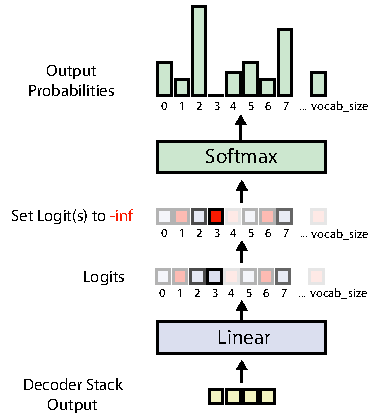
\includegraphics[width=.75\columnwidth]{figures/vulnerability_avoidance.pdf}
    \caption{Vulnerability-constrained decoding implementation.}
    \label{fig:vulnerability_avoidance_implementation}
\end{figure}


\subsubsection{Evaluate the performance of the vulnerability-constrained decoding}

To evaluate the performance of vulnerability-constrained decoding, the evaluation question is: \textbf{How well does the vulnerability-constrained decoding avoid generating vulnerable codes?} 

To answer this question, we follow the same approach as in \cref{sec:eval-security-synthesis}. However, we use the model after vulnerability-tuning and apply the vulnerability-constrained decoding method. We use the same samples as in \cref{sec:eval-performance-vulnerability-labeling-model}. If a sample is labeled correctly, we investigate whether the model using the vulnerability-constrained decoding approach avoided generating vulnerable codes.

As described in \cref{sec:eval-performance-vulnerability-labeling-model}, the model after vulnerability-tuning could label 58 samples correctly. Of these, the vulnerability-constrained decoding method can make 39 of these secure, while 19 remain vulnerable. This means 67\% of these vulnerabilities can be avoided using our vulnerability-constrained decoding approach. The distributions of the secure versus vulnerable codes generated are shown in \Cref{fig:secure_vs_vulnerable}.

\begin{figure}[htp]
    \centering
    %% Creator: Matplotlib, PGF backend
%%
%% To include the figure in your LaTeX document, write
%%   \input{<filename>.pgf}
%%
%% Make sure the required packages are loaded in your preamble
%%   \usepackage{pgf}
%%
%% Also ensure that all the required font packages are loaded; for instance,
%% the lmodern package is sometimes necessary when using math font.
%%   \usepackage{lmodern}
%%
%% Figures using additional raster images can only be included by \input if
%% they are in the same directory as the main LaTeX file. For loading figures
%% from other directories you can use the `import` package
%%   \usepackage{import}
%%
%% and then include the figures with
%%   \import{<path to file>}{<filename>.pgf}
%%
%% Matplotlib used the following preamble
%%   
%%   \makeatletter\@ifpackageloaded{underscore}{}{\usepackage[strings]{underscore}}\makeatother
%%
\begingroup%
\makeatletter%
\begin{pgfpicture}%
\pgfpathrectangle{\pgfpointorigin}{\pgfqpoint{3.267895in}{2.731592in}}%
\pgfusepath{use as bounding box, clip}%
\begin{pgfscope}%
\pgfsetbuttcap%
\pgfsetmiterjoin%
\definecolor{currentfill}{rgb}{1.000000,1.000000,1.000000}%
\pgfsetfillcolor{currentfill}%
\pgfsetlinewidth{0.000000pt}%
\definecolor{currentstroke}{rgb}{1.000000,1.000000,1.000000}%
\pgfsetstrokecolor{currentstroke}%
\pgfsetdash{}{0pt}%
\pgfpathmoveto{\pgfqpoint{0.000000in}{0.000000in}}%
\pgfpathlineto{\pgfqpoint{3.267895in}{0.000000in}}%
\pgfpathlineto{\pgfqpoint{3.267895in}{2.731592in}}%
\pgfpathlineto{\pgfqpoint{0.000000in}{2.731592in}}%
\pgfpathlineto{\pgfqpoint{0.000000in}{0.000000in}}%
\pgfpathclose%
\pgfusepath{fill}%
\end{pgfscope}%
\begin{pgfscope}%
\pgfsetbuttcap%
\pgfsetmiterjoin%
\definecolor{currentfill}{rgb}{1.000000,1.000000,1.000000}%
\pgfsetfillcolor{currentfill}%
\pgfsetlinewidth{0.000000pt}%
\definecolor{currentstroke}{rgb}{0.000000,0.000000,0.000000}%
\pgfsetstrokecolor{currentstroke}%
\pgfsetstrokeopacity{0.000000}%
\pgfsetdash{}{0pt}%
\pgfpathmoveto{\pgfqpoint{0.492360in}{0.654724in}}%
\pgfpathlineto{\pgfqpoint{3.167895in}{0.654724in}}%
\pgfpathlineto{\pgfqpoint{3.167895in}{2.357287in}}%
\pgfpathlineto{\pgfqpoint{0.492360in}{2.357287in}}%
\pgfpathlineto{\pgfqpoint{0.492360in}{0.654724in}}%
\pgfpathclose%
\pgfusepath{fill}%
\end{pgfscope}%
\begin{pgfscope}%
\pgfsetbuttcap%
\pgfsetroundjoin%
\definecolor{currentfill}{rgb}{0.000000,0.000000,0.000000}%
\pgfsetfillcolor{currentfill}%
\pgfsetlinewidth{0.803000pt}%
\definecolor{currentstroke}{rgb}{0.000000,0.000000,0.000000}%
\pgfsetstrokecolor{currentstroke}%
\pgfsetdash{}{0pt}%
\pgfsys@defobject{currentmarker}{\pgfqpoint{0.000000in}{-0.048611in}}{\pgfqpoint{0.000000in}{0.000000in}}{%
\pgfpathmoveto{\pgfqpoint{0.000000in}{0.000000in}}%
\pgfpathlineto{\pgfqpoint{0.000000in}{-0.048611in}}%
\pgfusepath{stroke,fill}%
}%
\begin{pgfscope}%
\pgfsys@transformshift{0.659581in}{0.654724in}%
\pgfsys@useobject{currentmarker}{}%
\end{pgfscope}%
\end{pgfscope}%
\begin{pgfscope}%
\definecolor{textcolor}{rgb}{0.000000,0.000000,0.000000}%
\pgfsetstrokecolor{textcolor}%
\pgfsetfillcolor{textcolor}%
\pgftext[x=0.690831in, y=0.366589in, left, base,rotate=90.000000]{\color{textcolor}\rmfamily\fontsize{9.000000}{10.800000}\selectfont DC}%
\end{pgfscope}%
\begin{pgfscope}%
\pgfsetbuttcap%
\pgfsetroundjoin%
\definecolor{currentfill}{rgb}{0.000000,0.000000,0.000000}%
\pgfsetfillcolor{currentfill}%
\pgfsetlinewidth{0.803000pt}%
\definecolor{currentstroke}{rgb}{0.000000,0.000000,0.000000}%
\pgfsetstrokecolor{currentstroke}%
\pgfsetdash{}{0pt}%
\pgfsys@defobject{currentmarker}{\pgfqpoint{0.000000in}{-0.048611in}}{\pgfqpoint{0.000000in}{0.000000in}}{%
\pgfpathmoveto{\pgfqpoint{0.000000in}{0.000000in}}%
\pgfpathlineto{\pgfqpoint{0.000000in}{-0.048611in}}%
\pgfusepath{stroke,fill}%
}%
\begin{pgfscope}%
\pgfsys@transformshift{0.994023in}{0.654724in}%
\pgfsys@useobject{currentmarker}{}%
\end{pgfscope}%
\end{pgfscope}%
\begin{pgfscope}%
\definecolor{textcolor}{rgb}{0.000000,0.000000,0.000000}%
\pgfsetstrokecolor{textcolor}%
\pgfsetfillcolor{textcolor}%
\pgftext[x=1.025273in, y=0.314872in, left, base,rotate=90.000000]{\color{textcolor}\rmfamily\fontsize{9.000000}{10.800000}\selectfont IOU}%
\end{pgfscope}%
\begin{pgfscope}%
\pgfsetbuttcap%
\pgfsetroundjoin%
\definecolor{currentfill}{rgb}{0.000000,0.000000,0.000000}%
\pgfsetfillcolor{currentfill}%
\pgfsetlinewidth{0.803000pt}%
\definecolor{currentstroke}{rgb}{0.000000,0.000000,0.000000}%
\pgfsetstrokecolor{currentstroke}%
\pgfsetdash{}{0pt}%
\pgfsys@defobject{currentmarker}{\pgfqpoint{0.000000in}{-0.048611in}}{\pgfqpoint{0.000000in}{0.000000in}}{%
\pgfpathmoveto{\pgfqpoint{0.000000in}{0.000000in}}%
\pgfpathlineto{\pgfqpoint{0.000000in}{-0.048611in}}%
\pgfusepath{stroke,fill}%
}%
\begin{pgfscope}%
\pgfsys@transformshift{1.328465in}{0.654724in}%
\pgfsys@useobject{currentmarker}{}%
\end{pgfscope}%
\end{pgfscope}%
\begin{pgfscope}%
\definecolor{textcolor}{rgb}{0.000000,0.000000,0.000000}%
\pgfsetstrokecolor{textcolor}%
\pgfsetfillcolor{textcolor}%
\pgftext[x=1.359715in, y=0.368383in, left, base,rotate=90.000000]{\color{textcolor}\rmfamily\fontsize{9.000000}{10.800000}\selectfont NC}%
\end{pgfscope}%
\begin{pgfscope}%
\pgfsetbuttcap%
\pgfsetroundjoin%
\definecolor{currentfill}{rgb}{0.000000,0.000000,0.000000}%
\pgfsetfillcolor{currentfill}%
\pgfsetlinewidth{0.803000pt}%
\definecolor{currentstroke}{rgb}{0.000000,0.000000,0.000000}%
\pgfsetstrokecolor{currentstroke}%
\pgfsetdash{}{0pt}%
\pgfsys@defobject{currentmarker}{\pgfqpoint{0.000000in}{-0.048611in}}{\pgfqpoint{0.000000in}{0.000000in}}{%
\pgfpathmoveto{\pgfqpoint{0.000000in}{0.000000in}}%
\pgfpathlineto{\pgfqpoint{0.000000in}{-0.048611in}}%
\pgfusepath{stroke,fill}%
}%
\begin{pgfscope}%
\pgfsys@transformshift{1.662907in}{0.654724in}%
\pgfsys@useobject{currentmarker}{}%
\end{pgfscope}%
\end{pgfscope}%
\begin{pgfscope}%
\definecolor{textcolor}{rgb}{0.000000,0.000000,0.000000}%
\pgfsetstrokecolor{textcolor}%
\pgfsetfillcolor{textcolor}%
\pgftext[x=1.694157in, y=0.375520in, left, base,rotate=90.000000]{\color{textcolor}\rmfamily\fontsize{9.000000}{10.800000}\selectfont RE}%
\end{pgfscope}%
\begin{pgfscope}%
\pgfsetbuttcap%
\pgfsetroundjoin%
\definecolor{currentfill}{rgb}{0.000000,0.000000,0.000000}%
\pgfsetfillcolor{currentfill}%
\pgfsetlinewidth{0.803000pt}%
\definecolor{currentstroke}{rgb}{0.000000,0.000000,0.000000}%
\pgfsetstrokecolor{currentstroke}%
\pgfsetdash{}{0pt}%
\pgfsys@defobject{currentmarker}{\pgfqpoint{0.000000in}{-0.048611in}}{\pgfqpoint{0.000000in}{0.000000in}}{%
\pgfpathmoveto{\pgfqpoint{0.000000in}{0.000000in}}%
\pgfpathlineto{\pgfqpoint{0.000000in}{-0.048611in}}%
\pgfusepath{stroke,fill}%
}%
\begin{pgfscope}%
\pgfsys@transformshift{1.997349in}{0.654724in}%
\pgfsys@useobject{currentmarker}{}%
\end{pgfscope}%
\end{pgfscope}%
\begin{pgfscope}%
\definecolor{textcolor}{rgb}{0.000000,0.000000,0.000000}%
\pgfsetstrokecolor{textcolor}%
\pgfsetfillcolor{textcolor}%
\pgftext[x=2.028599in, y=0.366589in, left, base,rotate=90.000000]{\color{textcolor}\rmfamily\fontsize{9.000000}{10.800000}\selectfont TD}%
\end{pgfscope}%
\begin{pgfscope}%
\pgfsetbuttcap%
\pgfsetroundjoin%
\definecolor{currentfill}{rgb}{0.000000,0.000000,0.000000}%
\pgfsetfillcolor{currentfill}%
\pgfsetlinewidth{0.803000pt}%
\definecolor{currentstroke}{rgb}{0.000000,0.000000,0.000000}%
\pgfsetstrokecolor{currentstroke}%
\pgfsetdash{}{0pt}%
\pgfsys@defobject{currentmarker}{\pgfqpoint{0.000000in}{-0.048611in}}{\pgfqpoint{0.000000in}{0.000000in}}{%
\pgfpathmoveto{\pgfqpoint{0.000000in}{0.000000in}}%
\pgfpathlineto{\pgfqpoint{0.000000in}{-0.048611in}}%
\pgfusepath{stroke,fill}%
}%
\begin{pgfscope}%
\pgfsys@transformshift{2.331790in}{0.654724in}%
\pgfsys@useobject{currentmarker}{}%
\end{pgfscope}%
\end{pgfscope}%
\begin{pgfscope}%
\definecolor{textcolor}{rgb}{0.000000,0.000000,0.000000}%
\pgfsetstrokecolor{textcolor}%
\pgfsetfillcolor{textcolor}%
\pgftext[x=2.363040in, y=0.364795in, left, base,rotate=90.000000]{\color{textcolor}\rmfamily\fontsize{9.000000}{10.800000}\selectfont TO}%
\end{pgfscope}%
\begin{pgfscope}%
\pgfsetbuttcap%
\pgfsetroundjoin%
\definecolor{currentfill}{rgb}{0.000000,0.000000,0.000000}%
\pgfsetfillcolor{currentfill}%
\pgfsetlinewidth{0.803000pt}%
\definecolor{currentstroke}{rgb}{0.000000,0.000000,0.000000}%
\pgfsetstrokecolor{currentstroke}%
\pgfsetdash{}{0pt}%
\pgfsys@defobject{currentmarker}{\pgfqpoint{0.000000in}{-0.048611in}}{\pgfqpoint{0.000000in}{0.000000in}}{%
\pgfpathmoveto{\pgfqpoint{0.000000in}{0.000000in}}%
\pgfpathlineto{\pgfqpoint{0.000000in}{-0.048611in}}%
\pgfusepath{stroke,fill}%
}%
\begin{pgfscope}%
\pgfsys@transformshift{2.666232in}{0.654724in}%
\pgfsys@useobject{currentmarker}{}%
\end{pgfscope}%
\end{pgfscope}%
\begin{pgfscope}%
\definecolor{textcolor}{rgb}{0.000000,0.000000,0.000000}%
\pgfsetstrokecolor{textcolor}%
\pgfsetfillcolor{textcolor}%
\pgftext[x=2.697482in, y=0.266667in, left, base,rotate=90.000000]{\color{textcolor}\rmfamily\fontsize{9.000000}{10.800000}\selectfont TOD}%
\end{pgfscope}%
\begin{pgfscope}%
\pgfsetbuttcap%
\pgfsetroundjoin%
\definecolor{currentfill}{rgb}{0.000000,0.000000,0.000000}%
\pgfsetfillcolor{currentfill}%
\pgfsetlinewidth{0.803000pt}%
\definecolor{currentstroke}{rgb}{0.000000,0.000000,0.000000}%
\pgfsetstrokecolor{currentstroke}%
\pgfsetdash{}{0pt}%
\pgfsys@defobject{currentmarker}{\pgfqpoint{0.000000in}{-0.048611in}}{\pgfqpoint{0.000000in}{0.000000in}}{%
\pgfpathmoveto{\pgfqpoint{0.000000in}{0.000000in}}%
\pgfpathlineto{\pgfqpoint{0.000000in}{-0.048611in}}%
\pgfusepath{stroke,fill}%
}%
\begin{pgfscope}%
\pgfsys@transformshift{3.000674in}{0.654724in}%
\pgfsys@useobject{currentmarker}{}%
\end{pgfscope}%
\end{pgfscope}%
\begin{pgfscope}%
\definecolor{textcolor}{rgb}{0.000000,0.000000,0.000000}%
\pgfsetstrokecolor{textcolor}%
\pgfsetfillcolor{textcolor}%
\pgftext[x=3.031924in, y=0.318422in, left, base,rotate=90.000000]{\color{textcolor}\rmfamily\fontsize{9.000000}{10.800000}\selectfont UpS}%
\end{pgfscope}%
\begin{pgfscope}%
\definecolor{textcolor}{rgb}{0.000000,0.000000,0.000000}%
\pgfsetstrokecolor{textcolor}%
\pgfsetfillcolor{textcolor}%
\pgftext[x=1.830128in,y=0.211111in,,top]{\color{textcolor}\rmfamily\fontsize{9.000000}{10.800000}\selectfont Vulnerability}%
\end{pgfscope}%
\begin{pgfscope}%
\pgfpathrectangle{\pgfqpoint{0.492360in}{0.654724in}}{\pgfqpoint{2.675535in}{1.702563in}}%
\pgfusepath{clip}%
\pgfsetrectcap%
\pgfsetroundjoin%
\pgfsetlinewidth{0.803000pt}%
\definecolor{currentstroke}{rgb}{0.690196,0.690196,0.690196}%
\pgfsetstrokecolor{currentstroke}%
\pgfsetdash{}{0pt}%
\pgfpathmoveto{\pgfqpoint{0.492360in}{0.654724in}}%
\pgfpathlineto{\pgfqpoint{3.167895in}{0.654724in}}%
\pgfusepath{stroke}%
\end{pgfscope}%
\begin{pgfscope}%
\pgfsetbuttcap%
\pgfsetroundjoin%
\definecolor{currentfill}{rgb}{0.000000,0.000000,0.000000}%
\pgfsetfillcolor{currentfill}%
\pgfsetlinewidth{0.803000pt}%
\definecolor{currentstroke}{rgb}{0.000000,0.000000,0.000000}%
\pgfsetstrokecolor{currentstroke}%
\pgfsetdash{}{0pt}%
\pgfsys@defobject{currentmarker}{\pgfqpoint{-0.048611in}{0.000000in}}{\pgfqpoint{-0.000000in}{0.000000in}}{%
\pgfpathmoveto{\pgfqpoint{-0.000000in}{0.000000in}}%
\pgfpathlineto{\pgfqpoint{-0.048611in}{0.000000in}}%
\pgfusepath{stroke,fill}%
}%
\begin{pgfscope}%
\pgfsys@transformshift{0.492360in}{0.654724in}%
\pgfsys@useobject{currentmarker}{}%
\end{pgfscope}%
\end{pgfscope}%
\begin{pgfscope}%
\definecolor{textcolor}{rgb}{0.000000,0.000000,0.000000}%
\pgfsetstrokecolor{textcolor}%
\pgfsetfillcolor{textcolor}%
\pgftext[x=0.330902in, y=0.611321in, left, base]{\color{textcolor}\rmfamily\fontsize{9.000000}{10.800000}\selectfont \(\displaystyle {0}\)}%
\end{pgfscope}%
\begin{pgfscope}%
\pgfpathrectangle{\pgfqpoint{0.492360in}{0.654724in}}{\pgfqpoint{2.675535in}{1.702563in}}%
\pgfusepath{clip}%
\pgfsetrectcap%
\pgfsetroundjoin%
\pgfsetlinewidth{0.803000pt}%
\definecolor{currentstroke}{rgb}{0.690196,0.690196,0.690196}%
\pgfsetstrokecolor{currentstroke}%
\pgfsetdash{}{0pt}%
\pgfpathmoveto{\pgfqpoint{0.492360in}{0.845487in}}%
\pgfpathlineto{\pgfqpoint{3.167895in}{0.845487in}}%
\pgfusepath{stroke}%
\end{pgfscope}%
\begin{pgfscope}%
\pgfsetbuttcap%
\pgfsetroundjoin%
\definecolor{currentfill}{rgb}{0.000000,0.000000,0.000000}%
\pgfsetfillcolor{currentfill}%
\pgfsetlinewidth{0.803000pt}%
\definecolor{currentstroke}{rgb}{0.000000,0.000000,0.000000}%
\pgfsetstrokecolor{currentstroke}%
\pgfsetdash{}{0pt}%
\pgfsys@defobject{currentmarker}{\pgfqpoint{-0.048611in}{0.000000in}}{\pgfqpoint{-0.000000in}{0.000000in}}{%
\pgfpathmoveto{\pgfqpoint{-0.000000in}{0.000000in}}%
\pgfpathlineto{\pgfqpoint{-0.048611in}{0.000000in}}%
\pgfusepath{stroke,fill}%
}%
\begin{pgfscope}%
\pgfsys@transformshift{0.492360in}{0.845487in}%
\pgfsys@useobject{currentmarker}{}%
\end{pgfscope}%
\end{pgfscope}%
\begin{pgfscope}%
\definecolor{textcolor}{rgb}{0.000000,0.000000,0.000000}%
\pgfsetstrokecolor{textcolor}%
\pgfsetfillcolor{textcolor}%
\pgftext[x=0.330902in, y=0.802084in, left, base]{\color{textcolor}\rmfamily\fontsize{9.000000}{10.800000}\selectfont \(\displaystyle {2}\)}%
\end{pgfscope}%
\begin{pgfscope}%
\pgfpathrectangle{\pgfqpoint{0.492360in}{0.654724in}}{\pgfqpoint{2.675535in}{1.702563in}}%
\pgfusepath{clip}%
\pgfsetrectcap%
\pgfsetroundjoin%
\pgfsetlinewidth{0.803000pt}%
\definecolor{currentstroke}{rgb}{0.690196,0.690196,0.690196}%
\pgfsetstrokecolor{currentstroke}%
\pgfsetdash{}{0pt}%
\pgfpathmoveto{\pgfqpoint{0.492360in}{1.036251in}}%
\pgfpathlineto{\pgfqpoint{3.167895in}{1.036251in}}%
\pgfusepath{stroke}%
\end{pgfscope}%
\begin{pgfscope}%
\pgfsetbuttcap%
\pgfsetroundjoin%
\definecolor{currentfill}{rgb}{0.000000,0.000000,0.000000}%
\pgfsetfillcolor{currentfill}%
\pgfsetlinewidth{0.803000pt}%
\definecolor{currentstroke}{rgb}{0.000000,0.000000,0.000000}%
\pgfsetstrokecolor{currentstroke}%
\pgfsetdash{}{0pt}%
\pgfsys@defobject{currentmarker}{\pgfqpoint{-0.048611in}{0.000000in}}{\pgfqpoint{-0.000000in}{0.000000in}}{%
\pgfpathmoveto{\pgfqpoint{-0.000000in}{0.000000in}}%
\pgfpathlineto{\pgfqpoint{-0.048611in}{0.000000in}}%
\pgfusepath{stroke,fill}%
}%
\begin{pgfscope}%
\pgfsys@transformshift{0.492360in}{1.036251in}%
\pgfsys@useobject{currentmarker}{}%
\end{pgfscope}%
\end{pgfscope}%
\begin{pgfscope}%
\definecolor{textcolor}{rgb}{0.000000,0.000000,0.000000}%
\pgfsetstrokecolor{textcolor}%
\pgfsetfillcolor{textcolor}%
\pgftext[x=0.330902in, y=0.992848in, left, base]{\color{textcolor}\rmfamily\fontsize{9.000000}{10.800000}\selectfont \(\displaystyle {4}\)}%
\end{pgfscope}%
\begin{pgfscope}%
\pgfpathrectangle{\pgfqpoint{0.492360in}{0.654724in}}{\pgfqpoint{2.675535in}{1.702563in}}%
\pgfusepath{clip}%
\pgfsetrectcap%
\pgfsetroundjoin%
\pgfsetlinewidth{0.803000pt}%
\definecolor{currentstroke}{rgb}{0.690196,0.690196,0.690196}%
\pgfsetstrokecolor{currentstroke}%
\pgfsetdash{}{0pt}%
\pgfpathmoveto{\pgfqpoint{0.492360in}{1.227014in}}%
\pgfpathlineto{\pgfqpoint{3.167895in}{1.227014in}}%
\pgfusepath{stroke}%
\end{pgfscope}%
\begin{pgfscope}%
\pgfsetbuttcap%
\pgfsetroundjoin%
\definecolor{currentfill}{rgb}{0.000000,0.000000,0.000000}%
\pgfsetfillcolor{currentfill}%
\pgfsetlinewidth{0.803000pt}%
\definecolor{currentstroke}{rgb}{0.000000,0.000000,0.000000}%
\pgfsetstrokecolor{currentstroke}%
\pgfsetdash{}{0pt}%
\pgfsys@defobject{currentmarker}{\pgfqpoint{-0.048611in}{0.000000in}}{\pgfqpoint{-0.000000in}{0.000000in}}{%
\pgfpathmoveto{\pgfqpoint{-0.000000in}{0.000000in}}%
\pgfpathlineto{\pgfqpoint{-0.048611in}{0.000000in}}%
\pgfusepath{stroke,fill}%
}%
\begin{pgfscope}%
\pgfsys@transformshift{0.492360in}{1.227014in}%
\pgfsys@useobject{currentmarker}{}%
\end{pgfscope}%
\end{pgfscope}%
\begin{pgfscope}%
\definecolor{textcolor}{rgb}{0.000000,0.000000,0.000000}%
\pgfsetstrokecolor{textcolor}%
\pgfsetfillcolor{textcolor}%
\pgftext[x=0.330902in, y=1.183611in, left, base]{\color{textcolor}\rmfamily\fontsize{9.000000}{10.800000}\selectfont \(\displaystyle {6}\)}%
\end{pgfscope}%
\begin{pgfscope}%
\pgfpathrectangle{\pgfqpoint{0.492360in}{0.654724in}}{\pgfqpoint{2.675535in}{1.702563in}}%
\pgfusepath{clip}%
\pgfsetrectcap%
\pgfsetroundjoin%
\pgfsetlinewidth{0.803000pt}%
\definecolor{currentstroke}{rgb}{0.690196,0.690196,0.690196}%
\pgfsetstrokecolor{currentstroke}%
\pgfsetdash{}{0pt}%
\pgfpathmoveto{\pgfqpoint{0.492360in}{1.417777in}}%
\pgfpathlineto{\pgfqpoint{3.167895in}{1.417777in}}%
\pgfusepath{stroke}%
\end{pgfscope}%
\begin{pgfscope}%
\pgfsetbuttcap%
\pgfsetroundjoin%
\definecolor{currentfill}{rgb}{0.000000,0.000000,0.000000}%
\pgfsetfillcolor{currentfill}%
\pgfsetlinewidth{0.803000pt}%
\definecolor{currentstroke}{rgb}{0.000000,0.000000,0.000000}%
\pgfsetstrokecolor{currentstroke}%
\pgfsetdash{}{0pt}%
\pgfsys@defobject{currentmarker}{\pgfqpoint{-0.048611in}{0.000000in}}{\pgfqpoint{-0.000000in}{0.000000in}}{%
\pgfpathmoveto{\pgfqpoint{-0.000000in}{0.000000in}}%
\pgfpathlineto{\pgfqpoint{-0.048611in}{0.000000in}}%
\pgfusepath{stroke,fill}%
}%
\begin{pgfscope}%
\pgfsys@transformshift{0.492360in}{1.417777in}%
\pgfsys@useobject{currentmarker}{}%
\end{pgfscope}%
\end{pgfscope}%
\begin{pgfscope}%
\definecolor{textcolor}{rgb}{0.000000,0.000000,0.000000}%
\pgfsetstrokecolor{textcolor}%
\pgfsetfillcolor{textcolor}%
\pgftext[x=0.330902in, y=1.374375in, left, base]{\color{textcolor}\rmfamily\fontsize{9.000000}{10.800000}\selectfont \(\displaystyle {8}\)}%
\end{pgfscope}%
\begin{pgfscope}%
\pgfpathrectangle{\pgfqpoint{0.492360in}{0.654724in}}{\pgfqpoint{2.675535in}{1.702563in}}%
\pgfusepath{clip}%
\pgfsetrectcap%
\pgfsetroundjoin%
\pgfsetlinewidth{0.803000pt}%
\definecolor{currentstroke}{rgb}{0.690196,0.690196,0.690196}%
\pgfsetstrokecolor{currentstroke}%
\pgfsetdash{}{0pt}%
\pgfpathmoveto{\pgfqpoint{0.492360in}{1.608541in}}%
\pgfpathlineto{\pgfqpoint{3.167895in}{1.608541in}}%
\pgfusepath{stroke}%
\end{pgfscope}%
\begin{pgfscope}%
\pgfsetbuttcap%
\pgfsetroundjoin%
\definecolor{currentfill}{rgb}{0.000000,0.000000,0.000000}%
\pgfsetfillcolor{currentfill}%
\pgfsetlinewidth{0.803000pt}%
\definecolor{currentstroke}{rgb}{0.000000,0.000000,0.000000}%
\pgfsetstrokecolor{currentstroke}%
\pgfsetdash{}{0pt}%
\pgfsys@defobject{currentmarker}{\pgfqpoint{-0.048611in}{0.000000in}}{\pgfqpoint{-0.000000in}{0.000000in}}{%
\pgfpathmoveto{\pgfqpoint{-0.000000in}{0.000000in}}%
\pgfpathlineto{\pgfqpoint{-0.048611in}{0.000000in}}%
\pgfusepath{stroke,fill}%
}%
\begin{pgfscope}%
\pgfsys@transformshift{0.492360in}{1.608541in}%
\pgfsys@useobject{currentmarker}{}%
\end{pgfscope}%
\end{pgfscope}%
\begin{pgfscope}%
\definecolor{textcolor}{rgb}{0.000000,0.000000,0.000000}%
\pgfsetstrokecolor{textcolor}%
\pgfsetfillcolor{textcolor}%
\pgftext[x=0.266667in, y=1.565138in, left, base]{\color{textcolor}\rmfamily\fontsize{9.000000}{10.800000}\selectfont \(\displaystyle {10}\)}%
\end{pgfscope}%
\begin{pgfscope}%
\pgfpathrectangle{\pgfqpoint{0.492360in}{0.654724in}}{\pgfqpoint{2.675535in}{1.702563in}}%
\pgfusepath{clip}%
\pgfsetrectcap%
\pgfsetroundjoin%
\pgfsetlinewidth{0.803000pt}%
\definecolor{currentstroke}{rgb}{0.690196,0.690196,0.690196}%
\pgfsetstrokecolor{currentstroke}%
\pgfsetdash{}{0pt}%
\pgfpathmoveto{\pgfqpoint{0.492360in}{1.799304in}}%
\pgfpathlineto{\pgfqpoint{3.167895in}{1.799304in}}%
\pgfusepath{stroke}%
\end{pgfscope}%
\begin{pgfscope}%
\pgfsetbuttcap%
\pgfsetroundjoin%
\definecolor{currentfill}{rgb}{0.000000,0.000000,0.000000}%
\pgfsetfillcolor{currentfill}%
\pgfsetlinewidth{0.803000pt}%
\definecolor{currentstroke}{rgb}{0.000000,0.000000,0.000000}%
\pgfsetstrokecolor{currentstroke}%
\pgfsetdash{}{0pt}%
\pgfsys@defobject{currentmarker}{\pgfqpoint{-0.048611in}{0.000000in}}{\pgfqpoint{-0.000000in}{0.000000in}}{%
\pgfpathmoveto{\pgfqpoint{-0.000000in}{0.000000in}}%
\pgfpathlineto{\pgfqpoint{-0.048611in}{0.000000in}}%
\pgfusepath{stroke,fill}%
}%
\begin{pgfscope}%
\pgfsys@transformshift{0.492360in}{1.799304in}%
\pgfsys@useobject{currentmarker}{}%
\end{pgfscope}%
\end{pgfscope}%
\begin{pgfscope}%
\definecolor{textcolor}{rgb}{0.000000,0.000000,0.000000}%
\pgfsetstrokecolor{textcolor}%
\pgfsetfillcolor{textcolor}%
\pgftext[x=0.266667in, y=1.755901in, left, base]{\color{textcolor}\rmfamily\fontsize{9.000000}{10.800000}\selectfont \(\displaystyle {12}\)}%
\end{pgfscope}%
\begin{pgfscope}%
\pgfpathrectangle{\pgfqpoint{0.492360in}{0.654724in}}{\pgfqpoint{2.675535in}{1.702563in}}%
\pgfusepath{clip}%
\pgfsetrectcap%
\pgfsetroundjoin%
\pgfsetlinewidth{0.803000pt}%
\definecolor{currentstroke}{rgb}{0.690196,0.690196,0.690196}%
\pgfsetstrokecolor{currentstroke}%
\pgfsetdash{}{0pt}%
\pgfpathmoveto{\pgfqpoint{0.492360in}{1.990067in}}%
\pgfpathlineto{\pgfqpoint{3.167895in}{1.990067in}}%
\pgfusepath{stroke}%
\end{pgfscope}%
\begin{pgfscope}%
\pgfsetbuttcap%
\pgfsetroundjoin%
\definecolor{currentfill}{rgb}{0.000000,0.000000,0.000000}%
\pgfsetfillcolor{currentfill}%
\pgfsetlinewidth{0.803000pt}%
\definecolor{currentstroke}{rgb}{0.000000,0.000000,0.000000}%
\pgfsetstrokecolor{currentstroke}%
\pgfsetdash{}{0pt}%
\pgfsys@defobject{currentmarker}{\pgfqpoint{-0.048611in}{0.000000in}}{\pgfqpoint{-0.000000in}{0.000000in}}{%
\pgfpathmoveto{\pgfqpoint{-0.000000in}{0.000000in}}%
\pgfpathlineto{\pgfqpoint{-0.048611in}{0.000000in}}%
\pgfusepath{stroke,fill}%
}%
\begin{pgfscope}%
\pgfsys@transformshift{0.492360in}{1.990067in}%
\pgfsys@useobject{currentmarker}{}%
\end{pgfscope}%
\end{pgfscope}%
\begin{pgfscope}%
\definecolor{textcolor}{rgb}{0.000000,0.000000,0.000000}%
\pgfsetstrokecolor{textcolor}%
\pgfsetfillcolor{textcolor}%
\pgftext[x=0.266667in, y=1.946665in, left, base]{\color{textcolor}\rmfamily\fontsize{9.000000}{10.800000}\selectfont \(\displaystyle {14}\)}%
\end{pgfscope}%
\begin{pgfscope}%
\pgfpathrectangle{\pgfqpoint{0.492360in}{0.654724in}}{\pgfqpoint{2.675535in}{1.702563in}}%
\pgfusepath{clip}%
\pgfsetrectcap%
\pgfsetroundjoin%
\pgfsetlinewidth{0.803000pt}%
\definecolor{currentstroke}{rgb}{0.690196,0.690196,0.690196}%
\pgfsetstrokecolor{currentstroke}%
\pgfsetdash{}{0pt}%
\pgfpathmoveto{\pgfqpoint{0.492360in}{2.180831in}}%
\pgfpathlineto{\pgfqpoint{3.167895in}{2.180831in}}%
\pgfusepath{stroke}%
\end{pgfscope}%
\begin{pgfscope}%
\pgfsetbuttcap%
\pgfsetroundjoin%
\definecolor{currentfill}{rgb}{0.000000,0.000000,0.000000}%
\pgfsetfillcolor{currentfill}%
\pgfsetlinewidth{0.803000pt}%
\definecolor{currentstroke}{rgb}{0.000000,0.000000,0.000000}%
\pgfsetstrokecolor{currentstroke}%
\pgfsetdash{}{0pt}%
\pgfsys@defobject{currentmarker}{\pgfqpoint{-0.048611in}{0.000000in}}{\pgfqpoint{-0.000000in}{0.000000in}}{%
\pgfpathmoveto{\pgfqpoint{-0.000000in}{0.000000in}}%
\pgfpathlineto{\pgfqpoint{-0.048611in}{0.000000in}}%
\pgfusepath{stroke,fill}%
}%
\begin{pgfscope}%
\pgfsys@transformshift{0.492360in}{2.180831in}%
\pgfsys@useobject{currentmarker}{}%
\end{pgfscope}%
\end{pgfscope}%
\begin{pgfscope}%
\definecolor{textcolor}{rgb}{0.000000,0.000000,0.000000}%
\pgfsetstrokecolor{textcolor}%
\pgfsetfillcolor{textcolor}%
\pgftext[x=0.266667in, y=2.137428in, left, base]{\color{textcolor}\rmfamily\fontsize{9.000000}{10.800000}\selectfont \(\displaystyle {16}\)}%
\end{pgfscope}%
\begin{pgfscope}%
\definecolor{textcolor}{rgb}{0.000000,0.000000,0.000000}%
\pgfsetstrokecolor{textcolor}%
\pgfsetfillcolor{textcolor}%
\pgftext[x=0.211111in,y=1.506005in,,bottom,rotate=90.000000]{\color{textcolor}\rmfamily\fontsize{9.000000}{10.800000}\selectfont Count}%
\end{pgfscope}%
\begin{pgfscope}%
\pgfpathrectangle{\pgfqpoint{0.492360in}{0.654724in}}{\pgfqpoint{2.675535in}{1.702563in}}%
\pgfusepath{clip}%
\pgfsetbuttcap%
\pgfsetmiterjoin%
\definecolor{currentfill}{rgb}{0.121569,0.466667,0.705882}%
\pgfsetfillcolor{currentfill}%
\pgfsetlinewidth{0.000000pt}%
\definecolor{currentstroke}{rgb}{0.000000,0.000000,0.000000}%
\pgfsetstrokecolor{currentstroke}%
\pgfsetstrokeopacity{0.000000}%
\pgfsetdash{}{0pt}%
\pgfpathmoveto{\pgfqpoint{0.575971in}{0.654724in}}%
\pgfpathlineto{\pgfqpoint{0.659581in}{0.654724in}}%
\pgfpathlineto{\pgfqpoint{0.659581in}{0.750106in}}%
\pgfpathlineto{\pgfqpoint{0.575971in}{0.750106in}}%
\pgfpathlineto{\pgfqpoint{0.575971in}{0.654724in}}%
\pgfpathclose%
\pgfusepath{fill}%
\end{pgfscope}%
\begin{pgfscope}%
\pgfpathrectangle{\pgfqpoint{0.492360in}{0.654724in}}{\pgfqpoint{2.675535in}{1.702563in}}%
\pgfusepath{clip}%
\pgfsetbuttcap%
\pgfsetmiterjoin%
\definecolor{currentfill}{rgb}{0.121569,0.466667,0.705882}%
\pgfsetfillcolor{currentfill}%
\pgfsetlinewidth{0.000000pt}%
\definecolor{currentstroke}{rgb}{0.000000,0.000000,0.000000}%
\pgfsetstrokecolor{currentstroke}%
\pgfsetstrokeopacity{0.000000}%
\pgfsetdash{}{0pt}%
\pgfpathmoveto{\pgfqpoint{0.910413in}{0.654724in}}%
\pgfpathlineto{\pgfqpoint{0.994023in}{0.654724in}}%
\pgfpathlineto{\pgfqpoint{0.994023in}{1.131632in}}%
\pgfpathlineto{\pgfqpoint{0.910413in}{1.131632in}}%
\pgfpathlineto{\pgfqpoint{0.910413in}{0.654724in}}%
\pgfpathclose%
\pgfusepath{fill}%
\end{pgfscope}%
\begin{pgfscope}%
\pgfpathrectangle{\pgfqpoint{0.492360in}{0.654724in}}{\pgfqpoint{2.675535in}{1.702563in}}%
\pgfusepath{clip}%
\pgfsetbuttcap%
\pgfsetmiterjoin%
\definecolor{currentfill}{rgb}{0.121569,0.466667,0.705882}%
\pgfsetfillcolor{currentfill}%
\pgfsetlinewidth{0.000000pt}%
\definecolor{currentstroke}{rgb}{0.000000,0.000000,0.000000}%
\pgfsetstrokecolor{currentstroke}%
\pgfsetstrokeopacity{0.000000}%
\pgfsetdash{}{0pt}%
\pgfpathmoveto{\pgfqpoint{1.244854in}{0.654724in}}%
\pgfpathlineto{\pgfqpoint{1.328465in}{0.654724in}}%
\pgfpathlineto{\pgfqpoint{1.328465in}{0.845487in}}%
\pgfpathlineto{\pgfqpoint{1.244854in}{0.845487in}}%
\pgfpathlineto{\pgfqpoint{1.244854in}{0.654724in}}%
\pgfpathclose%
\pgfusepath{fill}%
\end{pgfscope}%
\begin{pgfscope}%
\pgfpathrectangle{\pgfqpoint{0.492360in}{0.654724in}}{\pgfqpoint{2.675535in}{1.702563in}}%
\pgfusepath{clip}%
\pgfsetbuttcap%
\pgfsetmiterjoin%
\definecolor{currentfill}{rgb}{0.121569,0.466667,0.705882}%
\pgfsetfillcolor{currentfill}%
\pgfsetlinewidth{0.000000pt}%
\definecolor{currentstroke}{rgb}{0.000000,0.000000,0.000000}%
\pgfsetstrokecolor{currentstroke}%
\pgfsetstrokeopacity{0.000000}%
\pgfsetdash{}{0pt}%
\pgfpathmoveto{\pgfqpoint{1.579296in}{0.654724in}}%
\pgfpathlineto{\pgfqpoint{1.662907in}{0.654724in}}%
\pgfpathlineto{\pgfqpoint{1.662907in}{0.940869in}}%
\pgfpathlineto{\pgfqpoint{1.579296in}{0.940869in}}%
\pgfpathlineto{\pgfqpoint{1.579296in}{0.654724in}}%
\pgfpathclose%
\pgfusepath{fill}%
\end{pgfscope}%
\begin{pgfscope}%
\pgfpathrectangle{\pgfqpoint{0.492360in}{0.654724in}}{\pgfqpoint{2.675535in}{1.702563in}}%
\pgfusepath{clip}%
\pgfsetbuttcap%
\pgfsetmiterjoin%
\definecolor{currentfill}{rgb}{0.121569,0.466667,0.705882}%
\pgfsetfillcolor{currentfill}%
\pgfsetlinewidth{0.000000pt}%
\definecolor{currentstroke}{rgb}{0.000000,0.000000,0.000000}%
\pgfsetstrokecolor{currentstroke}%
\pgfsetstrokeopacity{0.000000}%
\pgfsetdash{}{0pt}%
\pgfpathmoveto{\pgfqpoint{1.913738in}{0.654724in}}%
\pgfpathlineto{\pgfqpoint{1.997349in}{0.654724in}}%
\pgfpathlineto{\pgfqpoint{1.997349in}{1.131632in}}%
\pgfpathlineto{\pgfqpoint{1.913738in}{1.131632in}}%
\pgfpathlineto{\pgfqpoint{1.913738in}{0.654724in}}%
\pgfpathclose%
\pgfusepath{fill}%
\end{pgfscope}%
\begin{pgfscope}%
\pgfpathrectangle{\pgfqpoint{0.492360in}{0.654724in}}{\pgfqpoint{2.675535in}{1.702563in}}%
\pgfusepath{clip}%
\pgfsetbuttcap%
\pgfsetmiterjoin%
\definecolor{currentfill}{rgb}{0.121569,0.466667,0.705882}%
\pgfsetfillcolor{currentfill}%
\pgfsetlinewidth{0.000000pt}%
\definecolor{currentstroke}{rgb}{0.000000,0.000000,0.000000}%
\pgfsetstrokecolor{currentstroke}%
\pgfsetstrokeopacity{0.000000}%
\pgfsetdash{}{0pt}%
\pgfpathmoveto{\pgfqpoint{2.248180in}{0.654724in}}%
\pgfpathlineto{\pgfqpoint{2.331790in}{0.654724in}}%
\pgfpathlineto{\pgfqpoint{2.331790in}{0.940869in}}%
\pgfpathlineto{\pgfqpoint{2.248180in}{0.940869in}}%
\pgfpathlineto{\pgfqpoint{2.248180in}{0.654724in}}%
\pgfpathclose%
\pgfusepath{fill}%
\end{pgfscope}%
\begin{pgfscope}%
\pgfpathrectangle{\pgfqpoint{0.492360in}{0.654724in}}{\pgfqpoint{2.675535in}{1.702563in}}%
\pgfusepath{clip}%
\pgfsetbuttcap%
\pgfsetmiterjoin%
\definecolor{currentfill}{rgb}{0.121569,0.466667,0.705882}%
\pgfsetfillcolor{currentfill}%
\pgfsetlinewidth{0.000000pt}%
\definecolor{currentstroke}{rgb}{0.000000,0.000000,0.000000}%
\pgfsetstrokecolor{currentstroke}%
\pgfsetstrokeopacity{0.000000}%
\pgfsetdash{}{0pt}%
\pgfpathmoveto{\pgfqpoint{2.582622in}{0.654724in}}%
\pgfpathlineto{\pgfqpoint{2.666232in}{0.654724in}}%
\pgfpathlineto{\pgfqpoint{2.666232in}{2.276212in}}%
\pgfpathlineto{\pgfqpoint{2.582622in}{2.276212in}}%
\pgfpathlineto{\pgfqpoint{2.582622in}{0.654724in}}%
\pgfpathclose%
\pgfusepath{fill}%
\end{pgfscope}%
\begin{pgfscope}%
\pgfpathrectangle{\pgfqpoint{0.492360in}{0.654724in}}{\pgfqpoint{2.675535in}{1.702563in}}%
\pgfusepath{clip}%
\pgfsetbuttcap%
\pgfsetmiterjoin%
\definecolor{currentfill}{rgb}{0.121569,0.466667,0.705882}%
\pgfsetfillcolor{currentfill}%
\pgfsetlinewidth{0.000000pt}%
\definecolor{currentstroke}{rgb}{0.000000,0.000000,0.000000}%
\pgfsetstrokecolor{currentstroke}%
\pgfsetstrokeopacity{0.000000}%
\pgfsetdash{}{0pt}%
\pgfpathmoveto{\pgfqpoint{2.917064in}{0.654724in}}%
\pgfpathlineto{\pgfqpoint{3.000674in}{0.654724in}}%
\pgfpathlineto{\pgfqpoint{3.000674in}{0.940869in}}%
\pgfpathlineto{\pgfqpoint{2.917064in}{0.940869in}}%
\pgfpathlineto{\pgfqpoint{2.917064in}{0.654724in}}%
\pgfpathclose%
\pgfusepath{fill}%
\end{pgfscope}%
\begin{pgfscope}%
\pgfpathrectangle{\pgfqpoint{0.492360in}{0.654724in}}{\pgfqpoint{2.675535in}{1.702563in}}%
\pgfusepath{clip}%
\pgfsetbuttcap%
\pgfsetmiterjoin%
\definecolor{currentfill}{rgb}{1.000000,0.498039,0.054902}%
\pgfsetfillcolor{currentfill}%
\pgfsetlinewidth{0.000000pt}%
\definecolor{currentstroke}{rgb}{0.000000,0.000000,0.000000}%
\pgfsetstrokecolor{currentstroke}%
\pgfsetstrokeopacity{0.000000}%
\pgfsetdash{}{0pt}%
\pgfpathmoveto{\pgfqpoint{0.659581in}{0.654724in}}%
\pgfpathlineto{\pgfqpoint{0.743192in}{0.654724in}}%
\pgfpathlineto{\pgfqpoint{0.743192in}{0.750106in}}%
\pgfpathlineto{\pgfqpoint{0.659581in}{0.750106in}}%
\pgfpathlineto{\pgfqpoint{0.659581in}{0.654724in}}%
\pgfpathclose%
\pgfusepath{fill}%
\end{pgfscope}%
\begin{pgfscope}%
\pgfpathrectangle{\pgfqpoint{0.492360in}{0.654724in}}{\pgfqpoint{2.675535in}{1.702563in}}%
\pgfusepath{clip}%
\pgfsetbuttcap%
\pgfsetmiterjoin%
\definecolor{currentfill}{rgb}{1.000000,0.498039,0.054902}%
\pgfsetfillcolor{currentfill}%
\pgfsetlinewidth{0.000000pt}%
\definecolor{currentstroke}{rgb}{0.000000,0.000000,0.000000}%
\pgfsetstrokecolor{currentstroke}%
\pgfsetstrokeopacity{0.000000}%
\pgfsetdash{}{0pt}%
\pgfpathmoveto{\pgfqpoint{0.994023in}{0.654724in}}%
\pgfpathlineto{\pgfqpoint{1.077634in}{0.654724in}}%
\pgfpathlineto{\pgfqpoint{1.077634in}{0.845487in}}%
\pgfpathlineto{\pgfqpoint{0.994023in}{0.845487in}}%
\pgfpathlineto{\pgfqpoint{0.994023in}{0.654724in}}%
\pgfpathclose%
\pgfusepath{fill}%
\end{pgfscope}%
\begin{pgfscope}%
\pgfpathrectangle{\pgfqpoint{0.492360in}{0.654724in}}{\pgfqpoint{2.675535in}{1.702563in}}%
\pgfusepath{clip}%
\pgfsetbuttcap%
\pgfsetmiterjoin%
\definecolor{currentfill}{rgb}{1.000000,0.498039,0.054902}%
\pgfsetfillcolor{currentfill}%
\pgfsetlinewidth{0.000000pt}%
\definecolor{currentstroke}{rgb}{0.000000,0.000000,0.000000}%
\pgfsetstrokecolor{currentstroke}%
\pgfsetstrokeopacity{0.000000}%
\pgfsetdash{}{0pt}%
\pgfpathmoveto{\pgfqpoint{1.328465in}{0.654724in}}%
\pgfpathlineto{\pgfqpoint{1.412075in}{0.654724in}}%
\pgfpathlineto{\pgfqpoint{1.412075in}{1.036251in}}%
\pgfpathlineto{\pgfqpoint{1.328465in}{1.036251in}}%
\pgfpathlineto{\pgfqpoint{1.328465in}{0.654724in}}%
\pgfpathclose%
\pgfusepath{fill}%
\end{pgfscope}%
\begin{pgfscope}%
\pgfpathrectangle{\pgfqpoint{0.492360in}{0.654724in}}{\pgfqpoint{2.675535in}{1.702563in}}%
\pgfusepath{clip}%
\pgfsetbuttcap%
\pgfsetmiterjoin%
\definecolor{currentfill}{rgb}{1.000000,0.498039,0.054902}%
\pgfsetfillcolor{currentfill}%
\pgfsetlinewidth{0.000000pt}%
\definecolor{currentstroke}{rgb}{0.000000,0.000000,0.000000}%
\pgfsetstrokecolor{currentstroke}%
\pgfsetstrokeopacity{0.000000}%
\pgfsetdash{}{0pt}%
\pgfpathmoveto{\pgfqpoint{1.662907in}{0.654724in}}%
\pgfpathlineto{\pgfqpoint{1.746517in}{0.654724in}}%
\pgfpathlineto{\pgfqpoint{1.746517in}{0.654724in}}%
\pgfpathlineto{\pgfqpoint{1.662907in}{0.654724in}}%
\pgfpathlineto{\pgfqpoint{1.662907in}{0.654724in}}%
\pgfpathclose%
\pgfusepath{fill}%
\end{pgfscope}%
\begin{pgfscope}%
\pgfpathrectangle{\pgfqpoint{0.492360in}{0.654724in}}{\pgfqpoint{2.675535in}{1.702563in}}%
\pgfusepath{clip}%
\pgfsetbuttcap%
\pgfsetmiterjoin%
\definecolor{currentfill}{rgb}{1.000000,0.498039,0.054902}%
\pgfsetfillcolor{currentfill}%
\pgfsetlinewidth{0.000000pt}%
\definecolor{currentstroke}{rgb}{0.000000,0.000000,0.000000}%
\pgfsetstrokecolor{currentstroke}%
\pgfsetstrokeopacity{0.000000}%
\pgfsetdash{}{0pt}%
\pgfpathmoveto{\pgfqpoint{1.997349in}{0.654724in}}%
\pgfpathlineto{\pgfqpoint{2.080959in}{0.654724in}}%
\pgfpathlineto{\pgfqpoint{2.080959in}{0.940869in}}%
\pgfpathlineto{\pgfqpoint{1.997349in}{0.940869in}}%
\pgfpathlineto{\pgfqpoint{1.997349in}{0.654724in}}%
\pgfpathclose%
\pgfusepath{fill}%
\end{pgfscope}%
\begin{pgfscope}%
\pgfpathrectangle{\pgfqpoint{0.492360in}{0.654724in}}{\pgfqpoint{2.675535in}{1.702563in}}%
\pgfusepath{clip}%
\pgfsetbuttcap%
\pgfsetmiterjoin%
\definecolor{currentfill}{rgb}{1.000000,0.498039,0.054902}%
\pgfsetfillcolor{currentfill}%
\pgfsetlinewidth{0.000000pt}%
\definecolor{currentstroke}{rgb}{0.000000,0.000000,0.000000}%
\pgfsetstrokecolor{currentstroke}%
\pgfsetstrokeopacity{0.000000}%
\pgfsetdash{}{0pt}%
\pgfpathmoveto{\pgfqpoint{2.331790in}{0.654724in}}%
\pgfpathlineto{\pgfqpoint{2.415401in}{0.654724in}}%
\pgfpathlineto{\pgfqpoint{2.415401in}{0.750106in}}%
\pgfpathlineto{\pgfqpoint{2.331790in}{0.750106in}}%
\pgfpathlineto{\pgfqpoint{2.331790in}{0.654724in}}%
\pgfpathclose%
\pgfusepath{fill}%
\end{pgfscope}%
\begin{pgfscope}%
\pgfpathrectangle{\pgfqpoint{0.492360in}{0.654724in}}{\pgfqpoint{2.675535in}{1.702563in}}%
\pgfusepath{clip}%
\pgfsetbuttcap%
\pgfsetmiterjoin%
\definecolor{currentfill}{rgb}{1.000000,0.498039,0.054902}%
\pgfsetfillcolor{currentfill}%
\pgfsetlinewidth{0.000000pt}%
\definecolor{currentstroke}{rgb}{0.000000,0.000000,0.000000}%
\pgfsetstrokecolor{currentstroke}%
\pgfsetstrokeopacity{0.000000}%
\pgfsetdash{}{0pt}%
\pgfpathmoveto{\pgfqpoint{2.666232in}{0.654724in}}%
\pgfpathlineto{\pgfqpoint{2.749843in}{0.654724in}}%
\pgfpathlineto{\pgfqpoint{2.749843in}{0.940869in}}%
\pgfpathlineto{\pgfqpoint{2.666232in}{0.940869in}}%
\pgfpathlineto{\pgfqpoint{2.666232in}{0.654724in}}%
\pgfpathclose%
\pgfusepath{fill}%
\end{pgfscope}%
\begin{pgfscope}%
\pgfpathrectangle{\pgfqpoint{0.492360in}{0.654724in}}{\pgfqpoint{2.675535in}{1.702563in}}%
\pgfusepath{clip}%
\pgfsetbuttcap%
\pgfsetmiterjoin%
\definecolor{currentfill}{rgb}{1.000000,0.498039,0.054902}%
\pgfsetfillcolor{currentfill}%
\pgfsetlinewidth{0.000000pt}%
\definecolor{currentstroke}{rgb}{0.000000,0.000000,0.000000}%
\pgfsetstrokecolor{currentstroke}%
\pgfsetstrokeopacity{0.000000}%
\pgfsetdash{}{0pt}%
\pgfpathmoveto{\pgfqpoint{3.000674in}{0.654724in}}%
\pgfpathlineto{\pgfqpoint{3.084285in}{0.654724in}}%
\pgfpathlineto{\pgfqpoint{3.084285in}{1.131632in}}%
\pgfpathlineto{\pgfqpoint{3.000674in}{1.131632in}}%
\pgfpathlineto{\pgfqpoint{3.000674in}{0.654724in}}%
\pgfpathclose%
\pgfusepath{fill}%
\end{pgfscope}%
\begin{pgfscope}%
\pgfsetrectcap%
\pgfsetmiterjoin%
\pgfsetlinewidth{0.803000pt}%
\definecolor{currentstroke}{rgb}{0.000000,0.000000,0.000000}%
\pgfsetstrokecolor{currentstroke}%
\pgfsetdash{}{0pt}%
\pgfpathmoveto{\pgfqpoint{0.492360in}{0.654724in}}%
\pgfpathlineto{\pgfqpoint{0.492360in}{2.357287in}}%
\pgfusepath{stroke}%
\end{pgfscope}%
\begin{pgfscope}%
\pgfsetrectcap%
\pgfsetmiterjoin%
\pgfsetlinewidth{0.803000pt}%
\definecolor{currentstroke}{rgb}{0.000000,0.000000,0.000000}%
\pgfsetstrokecolor{currentstroke}%
\pgfsetdash{}{0pt}%
\pgfpathmoveto{\pgfqpoint{0.492360in}{0.654724in}}%
\pgfpathlineto{\pgfqpoint{3.167895in}{0.654724in}}%
\pgfusepath{stroke}%
\end{pgfscope}%
\begin{pgfscope}%
\pgfsetbuttcap%
\pgfsetmiterjoin%
\definecolor{currentfill}{rgb}{0.121569,0.466667,0.705882}%
\pgfsetfillcolor{currentfill}%
\pgfsetlinewidth{0.000000pt}%
\definecolor{currentstroke}{rgb}{0.000000,0.000000,0.000000}%
\pgfsetstrokecolor{currentstroke}%
\pgfsetstrokeopacity{0.000000}%
\pgfsetdash{}{0pt}%
\pgfpathmoveto{\pgfqpoint{0.872984in}{2.494092in}}%
\pgfpathlineto{\pgfqpoint{1.122984in}{2.494092in}}%
\pgfpathlineto{\pgfqpoint{1.122984in}{2.581592in}}%
\pgfpathlineto{\pgfqpoint{0.872984in}{2.581592in}}%
\pgfpathlineto{\pgfqpoint{0.872984in}{2.494092in}}%
\pgfpathclose%
\pgfusepath{fill}%
\end{pgfscope}%
\begin{pgfscope}%
\definecolor{textcolor}{rgb}{0.000000,0.000000,0.000000}%
\pgfsetstrokecolor{textcolor}%
\pgfsetfillcolor{textcolor}%
\pgftext[x=1.222984in,y=2.494092in,left,base]{\color{textcolor}\rmfamily\fontsize{9.000000}{10.800000}\selectfont Secure}%
\end{pgfscope}%
\begin{pgfscope}%
\pgfsetbuttcap%
\pgfsetmiterjoin%
\definecolor{currentfill}{rgb}{1.000000,0.498039,0.054902}%
\pgfsetfillcolor{currentfill}%
\pgfsetlinewidth{0.000000pt}%
\definecolor{currentstroke}{rgb}{0.000000,0.000000,0.000000}%
\pgfsetstrokecolor{currentstroke}%
\pgfsetstrokeopacity{0.000000}%
\pgfsetdash{}{0pt}%
\pgfpathmoveto{\pgfqpoint{1.837372in}{2.494092in}}%
\pgfpathlineto{\pgfqpoint{2.087372in}{2.494092in}}%
\pgfpathlineto{\pgfqpoint{2.087372in}{2.581592in}}%
\pgfpathlineto{\pgfqpoint{1.837372in}{2.581592in}}%
\pgfpathlineto{\pgfqpoint{1.837372in}{2.494092in}}%
\pgfpathclose%
\pgfusepath{fill}%
\end{pgfscope}%
\begin{pgfscope}%
\definecolor{textcolor}{rgb}{0.000000,0.000000,0.000000}%
\pgfsetstrokecolor{textcolor}%
\pgfsetfillcolor{textcolor}%
\pgftext[x=2.187372in,y=2.494092in,left,base]{\color{textcolor}\rmfamily\fontsize{9.000000}{10.800000}\selectfont Vulnerable}%
\end{pgfscope}%
\end{pgfpicture}%
\makeatother%
\endgroup%

    \caption{Secure vs vulnerable result given correctly labeled.}
    \label{fig:secure_vs_vulnerable}
\end{figure}


By manual evaluations of the auto-completed code, we see some emerging patterns in the secure code produced by the model. Following are a few examples in which we show the diff between the generated code without and with vulnerability-constrained decoding. A horizontal line is inserted to indicate where the generation started. One of the most common patterns is the model cannot produce ``alternative secure code''. Instead, it produces whitespace characters. Around 50\% of the examples show this characteristic. An example of a TOD vulnerability can be seen in \Cref{lst:generated-tod-example}. A TOD vulnerability often requires a rewrite of the general contract logic. In this example, the vulnerability is correctly labeled with ``\textless TOD\textgreater''. However, as the model has been provided with substantial code context (not shown), it cannot generate alternative code and produces whitespace instead. As mentioned, to generate secure code in the first place, we believe it is better not to generate code rather than to generate vulnerable code.  

\newcommand{\lstbreak}{\break \raisebox{0ex}[0ex][0ex]{\ensuremath{\color{gray}\hookrightarrow\space}}}
\begin{lstlisting}[
    caption={TOD example.},
    label=lst:generated-tod-example,
    language=diff,
    belowskip=0pt,
    escapechar=§]
   function StopGame() public payable {
       require(msg.sender==questionSender);
\end{lstlisting}
\begin{lstlisting}[
    frame=bottomline,
    firstnumber=3,
    language=diff,
    aboveskip=0pt,
    escapechar=§]
 -     <TOD>msg.sender.transfer(this.balance);
 + §\lstbg{green!40}{\space\space\space\space}§
 + §\lstbg{green!40}{\space\space\space\space}§
 + §\lstbg{green!40}{\space\space\space\space}§
   }
\end{lstlisting}

\Cref{lst:generated-TD-RE-example} shows an example where the model generated more than whitespace characters. The generated code removed the vulnerabilities but could not provide a complete function. In this example, the model identified two vulnerabilities, both a TD at line 6 and a RE at line 8. It is also successful in removing them, mainly leaving lines 10 and 12 intact. However, in the process of removing the TD vulnerability, it also removes some checks of the ``acc.balance'' state variable. If a developer wants to keep the generated line 11 as a part of the function, the developer needs to add some checks to avoid a potential IOU vulnerability.  

\begin{lstlisting}[
    caption={TD and RE example.},
    label=lst:generated-TD-RE-example,
    language=diff,
    belowskip=0pt,
    escapechar=§]
   function Collect(uint _am)
   public
   payable
   {
       var acc = Acc[msg.sender];
\end{lstlisting}
\begin{lstlisting}[
    frame=bottomline,
    firstnumber=6,
    language=diff,
    aboveskip=0pt,
    escapechar=§]
 -     <TD>if( acc.balance>=MinSum && §\lstbreak§ acc.balance>=_am && now>acc.unlockTime)
 -     {
 -         <RE>if(msg.sender.call.value(_am)())
 -         {
 -     §\lstbg{red!40}{\space\space\space\space\space\space\space\space}§acc.balance-=_am;
 +     acc.balance-=_am;
 -     §\lstbg{red!40}{\space\space\space\space\space\space\space\space}§LogFile.AddMessage(msg.sender,_am,§\lstbreak§"Collect");
 +     LogFile.AddMessage(msg.sender,_am,"Collect");
 -         }
 -     }
   }
\end{lstlisting}

\Cref{lst:generated-TD-example} shows an example that the model generated a secure solution. In this example, the TD vulnerability has been marked with the ``\textless TD\textgreater'' label in line 2 due to the \lstinline{now} keyword. Using the vulnerability-constrained decoding, the model successfully avoids this keyword and instead relies on a state variable ``refundStatus''.

\begin{lstlisting}[
    caption={TD example.},
    label=lst:generated-TD-example,
    language=diff,
    belowskip=0pt,
    escapechar=§]
   function refund () public {
\end{lstlisting}
\begin{lstlisting}[
    frame=bottomline,
    firstnumber=2,
    language=diff,
    aboveskip=0pt,
    escapechar=§]
 -     §\lstbg{red!40}{<TD>}§require(§\lstbg{red!40}{now > icoFinish}§);
 +     require(§\lstbg{green!40}{refundStatus}§);
       require(contributorBalances[msg.sender]!= 0);
       uint refundValue = contributorBalances[msg.sender];
       contributorBalances[msg.sender] = 0;
       msg.sender.transfer(refundValue);
       emit Refund(msg.sender,refundValue);
   }
\end{lstlisting}


In summary, our experiments in sections \ref{sec:eval-security-synthesis} and \ref{sec:eval-performance-vulnerability-labeling-model} show that above 70\% of the code is vulnerable. Of this 70\%, we are able to correctly label 62\%, giving us a total labeling performance of 43\%. Of this 43\%, we can avoid 67\%. This gives us a total 30\% reduction of vulnerabilities. Combined with the secure baseline percentage of 30\%, our approach can increase the amount of secure code from 30\% to 60\%.

\subsubsection{Evaluate the impact on secure code generation} After vulnerability-tuning the model using the labeled vulnerable codes, it is also important to evaluate whether our vulnerability labeling fine-tuning has negatively impacted our model for generating code in secure cases. 

To answer this question, we follow a similar evaluation procedure as that in \Cref{sec:eval-quality-synthesis}. However, the generated code now contains vulnerability labels that are not present in our original SC testing dataset. We cut out any vulnerability tokens from the generated output to calculate the BLEU score. If the model performance is unaffected, we should expect a similar BLEU score as the results of the evaluation method in \cref{sec:eval-quality-synthesis}. We get a new BLEU score of 0.544, down from 0.557. This is a small performance decrease of 2.33\%, possibly due to the random nature of the models.

\section{Related Work}
\label{chap:related-work}

\newcommand*\emptycirc[1][1ex]{\tikz\draw (0,0) circle (#1);} 
\newcommand*\halfcirc[1][1ex]{%
  \begin{tikzpicture}
  \draw[fill] (0,0)-- (90:#1) arc (90:270:#1) -- cycle ;
  \draw (0,0) circle (#1);
  \end{tikzpicture}}
\newcommand*\fullcirc[1][1ex]{\tikz\fill (0,0) circle (#1);} 

One of the main problems with language models is that they often contain bias \cite{li2021detecting}, which can range from producing gender-specific jobs to favoring a certain race. In code synthesis, vulnerabilities can be considered a form of bias in language models. However, few studies focused on the security of synthesized code using transformers. Although \citet{chen2021codex} briefly discusses insecure code generated by Codex, the investigation was limited to exploring the generation of cryptography functions. While defenders can leverage new tools such as Security Copilot \cite{securitycopilot}, a Microsoft security analysis tool that enables analysts to respond to threats quickly, it is better to ensure code security in the first place, e.g., following principles like secure-by-construction \cite{securebyconstruction}.

Our approach has similarities with lexically-constrained decoding \cite{hokamp2017lexically}, which is a modification of the beam search that allows the user to specify tokens that must (or must not) appear in the decoder’s output. Post and Vilar \citet{post2018fast} proposed a variant of lexically-constrained decoding that reduced complexity from linear to constant-time, which was further optimized by \citet{hu2019improved}. While these works can deal with pre-defined constraints, our approach allows for embedding the constraint within the model through vulnerability-tuning. This enables more complex constraints, such as vulnerability patterns, to be avoided. By incorporating vulnerability-tuning, our approach can adapt and respond to changing constraints in real-time, offering enhanced flexibility and effectiveness. Furthermore, our implementation is based on a simple greedy search. We expect even better results using more complex decoding algorithms, such as beam-search, which are left for future investigations.

\Acrfull{rl} has been successfully used to align models according to human preferences \cite{ouyang2022training}. It is also known as \acrfull{rlhf} and powers ChatGPT \cite{chatgpt}. RL has also been applied to program synthesis. For example, \cite{le2022coderl} studied the integration of \acrshort{rl} with unit test signals in the fine-tuning of program synthesis models, and \cite{shojaee2023executionbased} further expanded on this idea, creating an \acrshort{rl} framework applicable to various code generation tasks and programming languages by employing execution feedback as an external source of knowledge in model optimization. Although \acrshort{rl} could be a strong candidate for reducing code vulnerabilities, it is a rather slow and resource-intensive process \cite{janner2021offline}. Unlike the \acrshort{rl}-based model fine-tuning, our approach prioritizes fast model updates to instantly mitigate the risk of generating vulnerable code. People can use our approach for quick and minor model updates. The slow and resource-intensive approaches, e.g., retraining the entire model using only secure code or the RLHF approach, are probably more suitable for major model updates.


\section{Discussion}
\label{chap:discussion}

In this section, we discuss the implications of our results and the threats to the validity of our study.

\subsection{Implication to academia and industry}
\label{sec:rq1-implication-to-academia-and-industry}

Vulnerabilities can be considered as a form of bias in language models. Hence, the vulnerability-constrained decoding approach could be generalized to handle other types of biases, such as gender bias. Since the approach relies primarily on augmenting the dataset, the method should also be transferable to other models. 

Existing code synthesis solutions based on transformers may produce many vulnerabilities \citet{pearch2021asleep}. Reducing vulnerabilities could bring significant benefits to the industry. Our results show that it is possible to quickly and incrementally fine-tune the code generator using information related to the vulnerabilities in the training dataset that are often gradually identified after the model is trained. This opens the possibilities for continuous model improvements to generate secure code. In this study, using only 941 labeled vulnerabilities to fine-tune the model within one hour has already significantly improved the model's capability to generate secure code. We believe fine-tuning the model with more vulnerability samples could further improve its performance.

The transformer model fine-tuned for SC code generation can accurately generate SC code with high BLEU and CrystalBLEU scores. Using this model in an industry setting can greatly reduce the efforts needed for creating SCs. Although Decrypted \cite{Decrypted} uses large-scale language models to generate SCs, it is in beta (since June 2021) and is close-sourced. There are no details about its model, training data, etc. 

A side product of the fine-tuned model is the construction of the currently largest dataset of real SCs, consisting of 186,397 SCs. The largest competing dataset \cite{ren2021empirical} contains 45,622 real-world SCs, filtered from 1.5 million contracts by comparing the MD5 hash of the contracts. However, their data are unfit for use in deep learning applications because they did not inflate the contracts to remove library code.

\subsection{Threats to validity}
\label{sec:rq1-threats-to-validity}

Many of the SCs contain duplicated code. If these duplications make up too large of a percentage of the dataset, this will lead to overly optimistic estimates of the model's performance. We performed an extensive filter of code duplications. Thus, we believe that the risk of cross-contamination in our study is relatively low.

A potential threat is that the manual classifications of the secure and vulnerable code may be biased. To mitigate the threat, all classifications of secure and vulnerable code are performed and cross-validated by two researchers. Another potential threat is the quality of the labeled data. Although we used the dataset of \cite{Hu2023}, which includes vulnerabilities that are verified by multiple code analysis tools with manual investigations, there are always false negatives and positives in the dataset, which may slightly impact our results. To evaluate the quality of the generated code, we use the BLEU and CrystalBLEU scores and leave alternative evaluation methods for SC code synthesis for future research.  

Concerning external validity, the approach does not rely on the specifics of SCs, other programming languages, or LLM models. However, since SCs are smaller and less complex than applications developed using other programming languages, there may be some restrictions on the generalizability of the approach.



\section{Conclusion and Future Work}
\label{chap:conclusion}

To address the issue that state-of-the-art LLMs generate vulnerabilities during code completion, we proposed a novel vulnerability-constrained decoding approach to drive the model to generate secure code. Our results provide the first empirical evidence that using static analysis tools to label vulnerable code and use them to fine-tune the model with the application of the vulnerability-constrained decoding approach can efficiently and effectively reduce the possibility of generating vulnerable code.

In the future, we plan to fine-tune the model with more vulnerable code samples to improve its performance. In addition, we want to investigate the possibility of using the model to label and auto-repair the vulnerable code typed in by the developers. 



\section{Data Availability}
\label{chap:data-availability}

We make all the SC datasets publicly available.
\begin{itemize}
    \item Verified Smart Contracts dataset:\\ \url{https://doi.org/10.6084/m9.figshare.20781799}
    \item Verified Smart Contract Code Comments dataset:\\ \url{https://doi.org/10.6084/m9.figshare.20780878}
    \item Vulnerable Verified Smart Contracts dataset:\\ \url{https://doi.org/10.6084/m9.figshare.21990287}
\end{itemize}

The final version of the SC model is also released.
\begin{itemize}
    \item Vulnerability-tuned GPT-J 6B model:\\ \url{https://doi.org/10.5281/zenodo.7595802}
\end{itemize}


\section*{Acknowledgments}
This work is jointly supported by the National Key Research and Development Program of China (No. 2019YFE0105500) and the Research Council of Norway (No. 309494) and the Key Research and Development Program of Jiangsu
Province (No. BE2021002-3). Tianyuan Hu thanks the Chinese Scholarship Council (CSC) for financial support (202106090057).



\chapter{Parameter-Efficient Fine-Tuning of Large Language Models for Unit Test Generation: An Empirical Study}


\section{Introduction}\label{sec1}
Training LLMs on extensive code bases like GitHub gives them seemingly magical capabilities. However, despite their proficiency in multiple code-related tasks, LLMs still struggle with the high cost of their training. The traditional approach to handling specialized tasks has been fine-tuning the model for each task. Given that LLMs often have billions, if not trillions, of parameters, traditional fine-tuning, which adjusts all parameters, is extremely computationally expensive and resource-intensive \citep{tufano2021unit}.

Advancements in LLMs have encouraged investigations into various prompting and tuning techniques, e.g., \citet{siddiq2024using, yuan2023manual, schäfer2023empirical}, that do not require full fine-tuning. This challenge has led to the development of multiple techniques for fine-tuning larger models with limited resources, commonly referred to as parameter-efficient fine-tuning (PEFT). The application of various PEFT methods has been explored for code-related tasks, such as code completion, code summarization, and more \citep{Ayupov2022ParameterEfficientFO, Goel2022OnTC, Wang2023PromptTI, weyssow2024exploring, Wang2023OneAF, Shi2023TowardsEF, Liu2023MFTCoderBC, yuan2023evaluating, Liu2023AnES}. Evaluations of the PEFT methods show that they could achieve performance comparable to full fine-tuning while significantly reducing the computational burden by strategically fine-tuning only a chosen subset of parameters for code-related tasks. However, the effectiveness of PEFT techniques on different tasks varies \citet{Ding2023ParameterefficientFO}. 

LLMs have been used to generate unit test cases and assertion statements \citep{Mastropaolo2021StudyingTU, yuan2023evaluating, siddiq2024using, yuan2023manual, schäfer2023empirical, tufano2021unit}. However, to the best of our knowledge, the area of empirical comparisons of PEFT and full fine-tuning for unit test generation remain unexplored. Therefore, in this work, we empirically evaluate the performance of various PEFT methods for unit test generation. We focus on answering the following research questions:
\begin{itemize} 

\item\textbf{RQ1: How well does PEFT perform on unit test generation?}
\item\textbf{RQ2: What is the relation between resource utilization and performance of PEFT in unit test generation?}

\end{itemize}

To answer the research questions, we compared full fine-tuning with three popular PEFT methods: LoRA (Low-Rank Adaptation) \citep{Yu2023LowRankAO}, (IA)\textsuperscript{3} (Infused Adapter by Inhibiting and Amplifying Inner Activations) \citep{Liu2022FewShotPF}, and prompt tuning \citep{Lester2021ThePO}. We conducted the comparisons using thirteen LLMs from four open-source decoder-only LLM families. The LLMs have varying architectures and sizes, ranging from 350 million to 16 billion parameters. We measured and compared the unit test generation performance of full fine-tuning and PEFT methods using well-established benchmark datasets rooted in real-world unit test cases and metrics, including syntactic correctness, CodeBLEU, pass@1, instruction coverage, branch coverage, and mutation score.

Our results show that LoRA is generally the most reliable PEFT method to generate good-quality unit tests and is, in many cases, on par with or even better than full fine-tuning. Regarding cost-effectiveness, prompt tuning provides the best results, particularly for larger models. Prompt tuning can be considered ``low-hanging fruit'', while LoRA should be employed for greater performance. The results also reveal that the generated unit tests from tuned models can contain more compilation errors, which need to be investigated in future studies.  
Our contributions are as follows:
\begin{itemize} 
    \item We conducted the first empirical study to extensively evaluate tuning LLMs using various PEFT methods—LoRA, (IA)\textsuperscript{3}, and prompt tuning—for unit test generation across a wide range of LLM models.
    \item We offered a comprehensive comparison of PEFT methods versus full fine-tuning.
    \item Our findings yield practical guidelines highlighting the potential gains and limitations of the various PEFT methods and full fine-tuning in resource utilization and performance.
\end{itemize}

The rest of the paper is organized as follows. \Cref{chap:peft-methods} introduces the PEFT methods we explore. \Cref{chap:related-work} introduces related work. We explain our experimental design in \Cref{chap:experimental-design}. \Cref{chap:experimental-results} presents the experimental results.  \Cref{chap:discussion} discusses our results and limitations. \Cref{chap:conclusion} concludes the study and proposes future work.

\section{PEFT Methods}
\label{chap:peft-methods}
Parameter-efficient fine-tuning (PEFT) methods provide an alternative way of fine-tuning a pre-trained model by training so-called adapters \citep{Ding2023ParameterefficientFO}. Here, most (if not all) parameters of the pre-trained model are frozen, and only a small number of parameters are trained. These adapters are often orders of magnitude smaller than the full model, making sharing, storing, and loading especially convenient. Moreover, some PEFT methods even facilitate the utilization of mixed-task batches, enabling distinct processing for different examples within a batch \citep{Lester2021ThePO}.
PEFT methods can be classified into three main categories: additive, selective, and reparametrization-based \citep{lialin2023scaling}. Additive methods can be further broken down into adapters \footnote{The term ``adapter'' is also used as the name of the first proposed adapter module for NLP.} and soft prompts.

\subsection{Additive}
This approach focuses on augmenting the pre-trained model with additional parameters or layers. Only the newly added components are trained, keeping the original model weights frozen. Popular techniques within the additive category are (IA)\textsuperscript{3} \citep{Liu2022FewShotPF}, adapters \citep{houlsby2019parameter}, and prompt tuning \citep{Lester2021ThePO}.

\paragraph{Adapters}
Adapter, or ``bottleneck adapter,'' introduced by \citet{houlsby2019parameter}, was arguably the first PEFT method. The class of ``adapters'' introduces small, fully connected networks placed after specific sub-layers within the model. These help the model adapt to the new task without significantly altering the core representation learned during pre-training.

\paragraph{Soft prompts}
These techniques focus on creating the so-called ``soft prompts.'' Prompt tuning, introduced by \citet{Lester2021ThePO}, fine-tuned a subset of the model's input embeddings, allowing the model to adapt to new tasks without altering the model's parameters. The prefix tuning expands the idea to all model layers \citep{li-liang-2021-prefix}. 

\subsection{Selective}
When using selective approaches, only a specific subset of the pre-trained model's parameters is fine-tuned. This approach requires carefully selecting the parameters to be updated, ensuring that they are most relevant to the new task. An example is BitFit by \citet{BenZaken2021BitFitSP}, which only updates the bias parameters.

\subsection{Reparametrization-based}
This category utilizes techniques that reformulate the original model's parameters into a more efficient trainable representation. This makes it possible to work with high-dimensional matrices while simultaneously reducing the number of trainable parameters. LoRA \citep{Yu2023LowRankAO} is a typical reparametrization-based method.

\section{Related Work}
\label{chap:related-work}
This section presents state-of-the-art studies generating unit tests using LLMs and studies applying PEFT approaches to enhance code-related tasks.  

\subsection{Unit test generation using LLMs}
\citet{tufano2021unit} propose an automated unit test case generation tool called \textsc{AthenaTest}. They construct a real-world focal method and developer-written test case dataset named \textsc{Methods2Test} \footnote{ https://github.com/microsoft/methods2test} and train a sequence-to-sequence transformer to generate unit test cases.
\citet{yuan2023manual} propose \textsc{ChatTester}, a ChatGPT-based unit test generation approach, which leverages ChatGPT itself to improve the quality of its generated tests. \citet{schäfer2023empirical} conducted a large-scale empirical evaluation on the effectiveness of LLMs for automated unit test generation without additional training. Similarly to \textsc{ChatTester}, they also use ChatGPT (GPT-3.5-Turbo) and propose a re-prompting approach named \textsc{TestPilot}. \textsc{TestPilot} automatically generates unit tests for all API functions in an npm package, achieving a median statement and branch coverage of 70.2\% and 52.8\% on 1,684 API functions, respectively. \citet{siddiq2024using} use the HumanEval and SF110 datasets to benchmark how well Codex, GPT-3.5-Turbo, and StarCoder can automatically generate unit tests. They evaluate the models based on compilation rates, test correctness, test coverage, and test smells. \citet{alagarsamy2024a3test} propose A3Test, a deep-learning based unit-test generation method that augments test generation with assertion knowledge and verifies naming and signatures. They evaluated the method on 5,278 focal methods from the Defects4J \citep{just2014defects4j} benchmark. The methods by \citet{yuan2023manual, siddiq2024using, schäfer2023empirical, alagarsamy2024a3test} primarily leverage large off-the-shelf LLMs, which can be costly and often lack the flexibility for custom fine-tuning to generate unit tests for specific domains and organizations. Additionally, such prompting-based methods often require significant manual effort to design complex templates and rely on expensive enterprise-grade LLMs like ChatGPT. 

\subsection{PEFT methods on code-related tasks}
Many cutting-edge methods for automatic code generation still involve computationally expensive full fine-tuning. One alternative approach to full fine-tuning is proposed by \citet{steenhoek2023reinforcement}. They use Reinforcement Learning from Static Quality Metrics (RLSQM). As reinforcement learning is a very expensive fine-tuning method, they also see the value of using PEFT methods like LoRA to facilitate the training.

PEFT has emerged as a powerful technique for enhancing code generation with LLMs. Researchers are investigating how to apply PEFT techniques to code-related tasks as a more efficient alternative to full fine-tuning. Results show that the effectiveness of PEFT techniques is task-dependent and not transferable. For example, \citet{Ayupov2022ParameterEfficientFO} evaluated adapters and LoRA on various tasks, finding them effective for code understanding but less so for code generation compared to full fine-tuning. \citet{Wang2023PromptTI} report that prompt tuning of CodeBERT and CodeT5 outperforms full fine-tuning for defect prediction, code summarization, and code translation tasks. \citet{Liu2023AnES} evaluated adapter, LoRA, Prefix tuning, and Mix-And-Match adapter (MAM) \citep{mam} for defect detection, code clone detection, and code summarization. They concluded that ``\textit{PEFT may achieve comparable or higher performance than full fine-tuning in code understanding tasks, but they may exhibit slightly weaker performance in code generation tasks.}'' Similarly, \citet{weyssow2024exploring} evaluated text-to-code generation using LoRA, (IA)\textsuperscript{3}, prompt tuning, and prefix tuning. They compared performance across models of varying sizes (up to 7 billion parameters) against full fine-tuning of smaller models (less than 350 million parameters) and concluded that LoRA is the most effective one.

As existing studies show that PEFT techniques' effectiveness is task-dependent, it is, therefore, necessary to empirically evaluate their effectiveness for unit test generation.  
To our knowledge, there is currently no systematic knowledge of how various PEFT methods behave to tune LLMs for unit test generation. In this study, we focus on autoregressive base code models to minimize the influence of prompt templates on PEFT performance.   

\section{Experimental design}
\label{chap:experimental-design}
The main objective of this study is to gain insight into the performance and cost-effectiveness of fine-tuning LLMs using PEFT for unit test generation.

\subsection{Research Questions}
To answer RQ1 (``\textbf{How well does PEFT perform on unit test generation?}''), we aim to evaluate several different PEFT methods on unit test generation. We also want to compare the PEFT methods with full fine-tuning. Thus, our study covers a wide range of language models for code of various sizes, spanning 350 million to 16 billion parameters. We assess the quality of the generated test cases by different PEFT methods by scoring against real-world human-written reference tests and evaluating the test cases' syntactic correctness, similarity to reference tests, passing rates, instruction and branch coverages, and mutation scores. Further, we examine whether applying PEFT methods for unit test generation adversely affects the pre-trained models' code generation performance, also known as catastrophic forgetting \citep{French1999CatastrophicFI, Luo2023AnES}. Organizations may use the same model to generate both code and unit tests within their integrated development environments (IDEs). This evaluation will help us understand if there are any trade-offs between applying fine-tuning and PEFT methods for unit test generation and maintaining performance on other code-related tasks.

To answer RQ2 (``\textbf{What is the relation between resource utilization and performance of PEFT in unit test generation?}''), we analyze the efficiency of PEFT methods in terms of the computational resources they use and the performance they achieve in unit test generation. 

\subsection{Fine-tuning methods selection}
In line with other empirical studies on PEFT \citep{weyssow2024exploring, Pu2023EmpiricalAO}, we select the most popularly used PEFT methods: LoRA \citep{Yu2023LowRankAO}, (IA)\textsuperscript{3} \citep{Liu2022FewShotPF}, and prompt tuning \citep{Lester2021ThePO}. They are readily available in popular libraries and exemplify most of the primary approaches within PEFT. 

\begin{figure*}[t]
    \centering
    \begin{subfigure}[t]{0.45\textwidth}
        \centering
        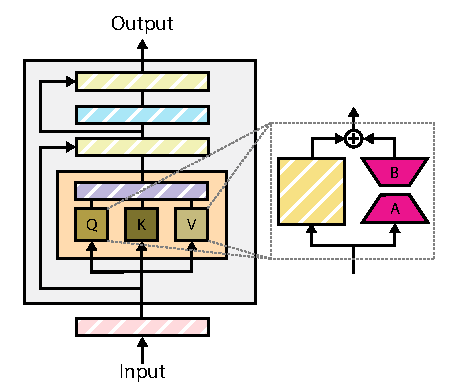
\includegraphics[scale=0.75,trim={0 -0.3375in 0 0}]{figures/lora.pdf}
        \caption{Diagram of LoRA (based on \citet{Yu2023LowRankAO}).}
        \label{fig:lora}
    \end{subfigure}%
    \hfill
    \begin{subfigure}[t]{0.27\textwidth}
        \centering
        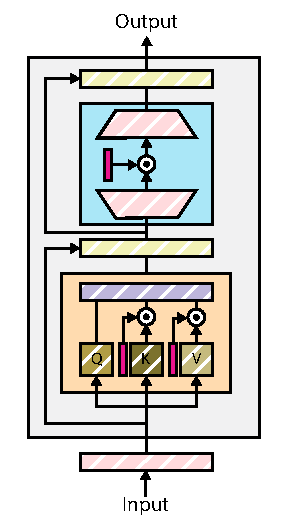
\includegraphics[scale=0.75]{figures/ia3.pdf}
        \caption{Diagram of (IA)\textsuperscript{3} (based on \citet{Liu2022FewShotPF}).}
        \label{fig:ia3}
    \end{subfigure}
    \hfill
    \begin{subfigure}[t]{0.27\textwidth}
        \centering
        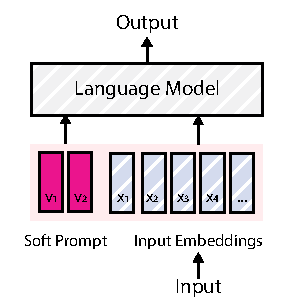
\includegraphics[scale=0.75,trim={0 -0.54in 0 0}]{figures/prompt_tuning.pdf}
        \caption{Diagram of prompt tuning (based on \citet{Lester2021ThePO}).}
        \label{fig:prompt-tuning}
    \end{subfigure}
    \caption{PEFT methods architecture illustration diagrams based on the reference implementation of each introductory paper. Striped modules are frozen. Magenta modules are trained.}
\end{figure*}

\begin{itemize}
    \item \textbf{LoRA}: A reparametrization-based method that updates a weight matrix by training a new matrix that is decomposed into a product of two matrices of lower rank: \(\delta W=W_A \cdot W_B\), where \(W_A \in \mathbb{R}^{\text{in} \times r}\) and \( W_B \in \mathbb{R}^{r \times \text{out}}\) \citep{Yu2023LowRankAO}. As demonstrated in \Cref{fig:lora}, the decomposed matrix is then added to the original frozen K and V projection matrices in the attention modules. All other modules are kept frozen.
    \item \textbf{(IA)\textsuperscript{3}}: An additive method that focuses on fine-tuning specific intermediate activations within the model \citep{Liu2022FewShotPF}. As illustrated in \Cref{fig:ia3}, this is done by learning three new vectors: \(l_v, l_k, l_{ff}\); rescaling key, value, and hidden feed-forward activations, respectively.
    \item \textbf{Prompt tuning}: A soft prompts (additive) method that fine-tunes a subset of the model's input embeddings. Exemplified in \Cref{fig:prompt-tuning}, the model input embeddings are prepended with a trainable tensor $P \in \mathbb{R}^{N \times D}$ (known as a ``soft prompt'') \citep{Lester2021ThePO}. Each element of \(P\) is also referred to as a ``virtual token.'' During training, these ``virtual tokens'' are updated while all the rest of the model parameters are kept frozen.
\end{itemize}

\subsection{Models}
\label{sec:models}
We select a diverse set of open-source autoregressive model families trained on code to evaluate the performance and cost-efficiency of PEFT methods. The chosen models span a range of sizes and architectures from the last four years, trained on diverse datasets and training objectives. This offers extensive insights into the interplay between various model capacities and PEFT methods. Further, all models are ensured to support the Java programming language to facilitate a fair comparison of our benchmarking datasets described in \Cref{sec:dataset}.

\begin{itemize}
\item \textbf{Salesforce CodeGen Models}: To democratize program synthesis, Salesforce AI Research developed CodeGen \citep{nijkamp2022codegen}. Pioneering in multi-turn program synthesis, CodeGen presents a variety of sizes, ranging from 350 million to 16 billion parameters. These models have undergone training across a diverse array of both programming and natural languages. The models were trained on ``The pile'' \citep{gao2020pile}, followed by a code subset of Google's BigQuery datasets \citep{GoogleBigQuery}. An updated version CodeGen2 \citep{nijkamp2023codegen2} is also available in sizes 1 billion to 16 billion, trained on ``The Stack'' dataset \citep{Kocetkov2022TheStack} using both causal language modeling (CLM) and file-level span corruption. We select the smallest model of the first generation CodeGen family (\textit{CodeGen-350M-multi}), along with all model sizes of the second generation (1 billion, 3.7 billion, 7 billion, and 16 billion parameters).

\item \textbf{Meta LLaMA Models}: Code Llama \citep{Rozire2023CodeLO}, derived from Llama 2 \citep{Touvron2023Llama2O}, is a specialized model further fine-tuned on the code-specific parts of its pre-training data. With enhanced coding capabilities, it can generate code, interpret natural language prompts, assist in code completion, and aid debugging. It comes in three variants. One is optimized for instructions. Another for Python. We select the base variant \textit{CodeLlama-7B}, as it is designed for general code synthesis and understanding and supports a wide range of popular languages, including Java.

\item \textbf{BigCode StarCoder Models}: This model family includes the 15.5 billion parameters \textit{StarCoderBase} model \citep{li2023starcoder}, along with an updated model generation named StarCoder2 \citep{Lozhkov2024StarCoder2A}, available in 3 billion, 7 billion, and 15 billion parameters. StarCoderBase was trained on 80+ programming languages from ``The Stack'' dataset \citep{Kocetkov2022TheStack}. The updated StarCoder2 is trained on 619 programming languages and other data sources, such as GitHub pull requests, Kaggle notebooks, and code docs. We select all model generations and sizes in this model family. 

\item \textbf{Qwen 2.5 Coder Models}: Qwen 2.5 Coder \citep{hui2024qwen} is the latest code-specific series of Qwen LLMs. The series comes in 0.5, 1.5, 3, 7, 14, 32 billion parameters. The models are built upon the Qwen2.5 architecture and pre-
trained on a vast corpus of over 5.5 trillion tokens. The dataset is sourced from a wide range of public code repositories, as well as large-scale web-crawled data containing code-related texts. We select the 3, 7 and 14 bllion parameter sizes of this model family. 
\end{itemize}

\Cref{tab:model-downloads} shows model statistics for the selected models derived from cfahlgren1/hub-stats hugging face dataset\footnote{\url{https://huggingface.co/datasets/cfahlgren1/hub-stats}} as of 13 November 2025. The chosen models span a representative set of model families released over the past four years, many of which remain highly popular.

\begin{table}[htbp]
    \newcolumntype{Y}{>{\centering\arraybackslash}X}
    \newcolumntype{R}{>{\raggedleft\arraybackslash}X}
    \centering
    \caption{HuggingFace model download statistics from cfahlgren1/hub-stats dataset as of 13 November 2025.}
    \label{tab:model-downloads}
    \small
    \begin{tabularx}{\columnwidth}{lRRY}
    \toprule
    \textbf{Model} & \textbf{Downloads in October 2025} & \textbf{Downloads all time} & \textbf{Created at} \\
    \midrule
    Qwen/Qwen2.5-Coder-14B & 4621 & 185216 & 2024-11-08 \\
    Qwen/Qwen2.5-Coder-3B & 15469 & 213837 & 2024-11-08 \\
    Qwen/Qwen2.5-Coder-7B & 22839 & 453481 & 2024-09-16 \\
    meta-llama/CodeLlama-7b-hf & 2274 & 200519 & 2024-03-13 \\
    bigcode/starcoder2-7b & 17013 & 695181 & 2024-02-20 \\
    bigcode/starcoder2-15b & 5397 & 450456 & 2024-02-20 \\
    bigcode/starcoder2-3b & 192177 & 6168133 & 2023-11-29 \\
    bigcode/starcoderbase & 7185 & 210970 & 2023-05-03 \\
    Salesforce/codegen2-16B\_P & 13 & 37908 & 2023-04-26 \\
    Salesforce/codegen2-7B\_P & 90 & 28639 & 2023-04-26 \\
    Salesforce/codegen2-3\_7B\_P & 42 & 39302 & 2023-04-25 \\
    Salesforce/codegen2-1B\_P & 226 & 77365 & 2023-04-25 \\
    Salesforce/codegen-350M-multi & 4113 & 588888 & 2022-04-11 \\
    \bottomrule
    \end{tabularx}
\end{table}

\subsection{Datasets}
\label{sec:dataset}
\subsubsection{\textsc{Methods2Test\textsubscript{small}}}
To ensure our experiments' validity and practical applicability, we rely on \textsc{Methods2Test} by \citet{tufano2021unit}. It is the largest publicly available corpus of Java unit test cases and corresponding focal methods. This dataset contains 780,000 test cases sourced from 91,000 open-source repositories on GitHub. These real-world test cases represent the complexity and variability inherent in software development, making them an ideal choice for evaluating automated test generation methods. By leveraging \textsc{Methods2Test}, we can assess the performance of the various PEFT methods and models in generating high-quality unit tests that align with real-world coding practices and challenges.

One of the advantages promised by various PEFT methods is the reduction in the amount of data needed for effective training. Thus, we opt to downsize the \textsc{Methods2Test} dataset to enhance efficiency without compromising the representativeness of the data. Specifically, we adopt a strategy wherein only one focal function is selected at random from each class in the dataset. By doing so, we maintain the essence and diversity of the original dataset while significantly reduce its size. Further, the \textsc{Methods2Test} dataset is distributed in deconstructed components. Hence, we assemble it according to the structure seen in \Cref{lst:data-structure} and package it as \textsc{Methods2Test\textsubscript{small}}. The resulting dataset contains 7440 training, 953 validation, and 1017 testing tests. We use this as the primary training dataset.

\subsubsection{\textsc{Methods2Test\textsubscript{runnable}}}
\label{sec:methods2test-runnable}
As the \textsc{Methods2Test} dataset is made up of tests from the real world, executing the tests to measure their passing rates, test coverages, and mutation scores needs significant extra work. This includes retrieving the correct repository version, resolving dependencies, injecting coverage collection tools and mutation testing systems into the existing build system, and finally executing the code in a controlled and safe manner. We construct a runnable subset of \textsc{Methods2Test} by the following steps: 1)  \textbf{Golden commit}: \textsc{Methods2Test} does not provide the repository commits at the time of scraping. Therefore, for each repository, we consider all commits prior to the last commit\footnote{\url{https://github.com/microsoft/methods2test/commit/309ee31cb3752cd8f3ad4b33cfd2b6e5b0ec5029}} on GitHub that updated the Methods2Test dataset (2021-05-18T23:18:51.000Z UTC) in which the focal method and test class files exist as candidate commits. We brute force (begin at the most recent candidate commit and iteratively check older commits)  compare all available dataset data against the repository until we find an exact match---a golden commit. 2) \textbf{Build system}: We target repositories using the Maven build system \citep{apache-maven:3.8.1}, as this is somewhat structured and not as flexible as Gradle. We rely on build file names to determine the build system. Of the 1017 tests in the test split of \textsc{Methods2Test\textsubscript{small}}, 624 of the repositories in \textsc{Methods2Test} are using Maven, 264 are using Gradle, and 129 are using others. 3) \textbf{Runnable}: Each repository in \textsc{Methods2Test}'s test split is then checked for buildability by running Maven and executing the test split of \textsc{Methods2Test\textsubscript{small}}. Due to a lot of old and missing dependencies, only 119 of the 624 Maven repositories are buildable. We collect all tests from \textsc{Methods2Test} with buildable repositories, resulting in 6150 tests. We then validate their runnability by executing every test, obtaining 3712 runnable tests (see \cref{sec:test-execution} for additional test execution details.) 
4) \textbf{Assertion heuristic}: Finally, we filter out any tests that do not contain any of the substrings  ``\texttt{assert}'', ``\texttt{verify}'', or ``\texttt{fail}''. These substrings are common indicators of meaningful test logic in Java-based testing frameworks. Tests lacking these keywords are often empty, incomplete, disabled, or rely on custom test runners and frameworks that bypass standard test assertions. To avoid misleading results—such as treating a test that silently does nothing as correct—we conservatively discard such test cases. This results in a total of 3266 runnable tests. We package it as \textsc{Methods2Test\textsubscript{runnable}}. We use this as the primary testing dataset.
\noindent We package the commit, build system, and execution status as \textsc{Methods2Test\textsubscript{meta}}.

\makeatletter
\newcommand{\gettikzxy}[3]{%
  \tikz@scan@one@point\pgfutil@firstofone#1\relax
  \edef#2{\the\pgf@x}%
  \edef#3{\the\pgf@y}%
}
\makeatother

\newcommand*{\drawBrace}[5][0pt]{%
    \gettikzxy{(pic cs:#3)}{\ax}{\ay}
    \gettikzxy{(pic cs:#4)}{\bx}{\by}
    \draw [decorate,decoration={brace,amplitude=4pt,aspect=#2}]
    (#1,\ay) --(#1,\by) node[pos=#2, right, font=\footnotesize, xshift=4pt] {#5};
    
}%

\definecolor{mygreen}{rgb}{0,0.6,0}
\definecolor{mygray}{rgb}{0.5,0.5,0.5}
\definecolor{mymauve}{rgb}{0.58,0,0.82}

\lstset{ %
  backgroundcolor=\color{white},   % choose the background color
  basicstyle=\footnotesize,        % size of fonts used for the code
  breaklines=true,                 % automatic line breaking only at whitespace
  captionpos=b,                    % sets the caption-position to bottom
  commentstyle=\color{mygreen},    % comment style
  escapeinside={\%*}{*)},          % if you want to add LaTeX within your code
  keywordstyle=\color{blue},       % keyword style
  stringstyle=\color{mymauve},     % string literal style
}

\begin{lstlisting}[
    float=!htb,
    name=listing,
    escapechar=!,
    language=java,
    caption={Dataset components: focal method (\textit{fm}), focal class name (\textit{fc}), constructor signatures (\textit{c}), method signatures(\textit{m}), fields (\textit{f}), test case (\textit{t}), test class name (\textit{tc}). Data is assembeld according to \textit{fm}+\textit{fc}+\textit{c}+\textit{m}+\textit{f}+\textit{t}+\textit{tc}. The code is split after the test case signature. Everything above the red line is the \textit{source} input for unit test generation. The code below the red line is the \textit{target} output of the unit test generation.},
    label={lst:data-structure}
    ]
// Focal class
public class Calculator {!\tikzmark{bgnfm}\tikzmark{bgnfc}\tikzmark{bgnc}\tikzmark{bgnm}\tikzmark{bgnf}!

    // Focal method
    public float add(float value) {!\tikzmark{bgnfm}!
        this.previousValue = this.currentValue;
        this.currentValue += value;
        return this.currentValue;
    }!\tikzmark{trmfm}\tikzmark{trmfc}\tikzmark{trmc}!

    // Constructor signatures
    public Calculator();
    public Calculator(float value);!\tikzmark{trmc}!

    // Method signatures
    public float subtract(float value);
    public float multiply(float value);
    public float divide(float value);
    public void reset();!\tikzmark{trmm}!

    // Fields
    public float currentValue;
    public float previousValue;
}!\tikzmark{trmf}!

// Test class
public class CalculatorTest {!\tikzmark{bgntc}!

    // Test case
    @Test!\tikzmark{bgnt}!
    public void testAdd() {
    !\tikzmark{split}!
        Calculator calc = new Calculator();
        assertEquals(5.0, calc.add(5.0f), 0.001);
        assertEquals(7.0, calc.add(2.0f), 0.001);
    }!\tikzmark{trmt}\tikzmark{trmtc}!
}!\begin{tikzpicture}[overlay, remember picture]
    \drawBrace[8.395*1.05]{0.5}{bgnfm}{trmfm}{\textit{fm}};
    \drawBrace[9.45*1.05]{0.72}{bgnfc}{trmfc}{+\textit{fc}};
    \drawBrace[10.4895*1.05]{0.46}{bgnc}{trmc}{+\textit{c}};
    \drawBrace[11.5475*1.05]{0.3}{bgnm}{trmm}{+\textit{m}};
    \drawBrace[12.6*1.05]{0.23}{bgnf}{trmf}{+\textit{f}};
    \drawBrace[8.39*1.05]{0.5}{bgnt}{trmt}{\textit{t}};
    \drawBrace[9.45*1.05]{0.675}{bgntc}{trmtc}{+\textit{tc}};
    %\iftikzmark{line-code-1-start}{\fill[red,overlay] (pic cs:line-code-1-start) circle[radius=4pt];}{\message{No start for 1}}
    %\drawBrace[0pt]{0.2}{bgnfc}{trmfc}{+fc};

    \gettikzxy{(pic cs:split)}{\ax}{\ay}
    \draw[red,thick,xshift=-3pt,yshift=1pt] (0,\ay) -- (\columnwidth,\ay) node[black,pos=.95,below] {\small Target} node[black,pos=.95,above] {\small Source};
\end{tikzpicture}!
\end{lstlisting}

\subsubsection{HumanEval-X}
HumanEval is a benchmarking dataset for code generation, first introduced by \citet{Chen2021EvaluatingLL}. It consists of 164 hand-written programming problems written in Python. For each programming problem, a function signature, docstring, body, and several unit tests are provided. \citet{Zheng2023CodeGeeXAP} extended the dataset to multiple languages, named HumanEval-X. We use the Java subset of the HumanEval-X dataset to evaluate potential catastrophic forgetting effects of fine-tuning.

\subsection{Training}
As the training dataset \textsc{Methods2Test\textsubscript{small}} only includes method signatures for non-focal methods, the unit test generation task can be considered a sequence-to-sequence (seq2seq) problem. Thus, to preserve the code completion capabilities of the decoder-only models described in \Cref{sec:models}, we model the seq2seq task as an autoregressive problem. This is done by only calculating loss based on the \textit{target} code, i.e., the unit test code. We minimize the following autoregressive cross-entropy loss function:
\begin{equation}
\mathcal{L} = - \sum_{t=1}^{T} \mathds{1}_t \cdot \log p(x_t \mid x_{1:t-1}),
\end{equation}
where:
\begin{equation}
\mathds{1}_i = 
\begin{cases}
    1, & \text{if } x_i \neq -100\\
    0, & \text{otherwise}.
\end{cases}
\end{equation}

The model is fed the \textit{source} and \textit{target} concatenated together (see  \Cref{lst:data-structure}). The token values for the \textit{source} are set to -100. The indicator function $\mathds{1}_i$ is used to ignore the \textit{source} in the loss computation.

\begin{table}[htb]
    \centering
    \caption{Model-agnostic hyperparameters for training.}\label{tab:hyperparameters-training}
    \newcolumntype{Y}{>{\centering\arraybackslash}X}
    \small
    \begin{tabularx}{\textwidth}{llY}
        \toprule
        \textbf{Hyperparameter} & \textbf{Method} & \textbf{Value}\\
        \midrule
        \multicolumn{3}{l}{\cellcolor{gray!10}{\textbf{Common}}} \bigstrut \\*
        Optimizer & - &  AdamW \\
        LR schedule & - &  Linear \\
        LR warmup ratio & - &  0.1 \\
        Batch size & - &  1 \\
        Gradient accumulation steps & - &  8 \\
        \# Epochs & - &  3 \\
        Precision & - &  Mixed\\
        \midrule
        \multirow{4}{*}{Learning rate} & Full fine-tuning & 5E-5\\
        & LoRA & 3E-4 \\
        & (IA)\textsuperscript{3} & 3E-4\\
        & Prompt tuning & 3E-3 \\
        \multicolumn{3}{l}{\cellcolor{gray!10}{\textbf{Method specific}}} \bigstrut \\*
        Alpha & LoRA & 32 \\
        Dropout & LoRA & 0.1 \\
        Rank & LoRA & 16 \\
        Virtual tokens & Prompt tuning & 20 \\
       \bottomrule
    \end{tabularx}
\end{table}

\begin{table}[htb]
    \centering
    \small
    \caption{Model-specific hyperparameters for training.}\label{tab:model-specific-hyperparameters-training}
    \begin{tabularx}{\textwidth}{p{3cm}Xll}
        \toprule
        \textbf{Hyperparameter} & \textbf{Method} & \textbf{Model} & \textbf{Value}\\
        \midrule
        \multirow{10}{3cm}{Targeted attention modules} & \multirow{10}{*}{LoRA, (IA)\textsuperscript{3}} & Salesforce/codegen-350M-multi & qkv\_proj \\
        & & Salesforce/codegen2-1B\_P & qkv\_proj \\
        & & Salesforce/codegen2-3\_7B\_P & qkv\_proj \\
        & & Salesforce/codegen2-7B\_P & qkv\_proj \\
        & & Salesforce/codegen2-16B\_P & qkv\_proj \\
        & & meta-llama/CodeLlama-7b-hf & q\_proj, v\_proj \\
        & & bigcode/starcoderbase & c\_attn \\
        & & bigcode/starcoder2-3b & q\_proj, v\_proj \\
        & & bigcode/starcoder2-7b & q\_proj, v\_proj \\
        & & bigcode/starcoder2-15b & q\_proj, v\_proj \\
        & & Qwen/Qwen2.5-Coder-3B & q\_proj,v\_proj \\
        & & Qwen/Qwen2.5-Coder-7B & q\_proj,v\_proj \\
        & & Qwen/Qwen2.5-Coder-14B & q\_proj,v\_proj \\
        \midrule
        \multirow{10}{3cm}{Targeted feedforward modules} & \multirow{10}{*}{(IA)\textsuperscript{3}} & Salesforce/codegen-350M-multi & fc\_out \\
        & & Salesforce/codegen2-1B\_P & fc\_out \\
        & & Salesforce/codegen2-3\_7B\_P & fc\_out \\
        & & Salesforce/codegen2-7B\_P & fc\_out \\
        & & Salesforce/codegen2-16B\_P & fc\_out \\
        & & meta-llama/CodeLlama-7b-hf & down\_proj \\
        & & bigcode/starcoderbase & mlp.c\_proj \\
        & & bigcode/starcoder2-3b & q\_proj, c\_proj \\
        & & bigcode/starcoder2-7b & q\_proj, c\_proj \\
        & & bigcode/starcoder2-15b & q\_proj, c\_proj \\
        & & Qwen/Qwen2.5-Coder-3B & down\_proj \\
        & & Qwen/Qwen2.5-Coder-7B & down\_proj \\
        & & Qwen/Qwen2.5-Coder-14B & down\_proj \\
       \bottomrule
    \end{tabularx}
\end{table}

We use the Transformers \citep{wolf-etal-2020-transformers} and PEFT libraries \citep{peft} from Hugging Face to conduct all training. We use NVIDIA A100 GPUs and leverage DeepSpeed ZeRO-Offload \citep{Ren2021ZeROOffloadDB} where necessary. We use the hyperparameters shown in \Cref{tab:hyperparameters-training} for training. Like other studies, e.g. that of \citet{weyssow2024exploring}, we select hyperparameter values that align with those specified in the original papers of the respective PEFT techniques. \citet{weyssow2024exploring} fine-tuned their models for up to five epochs. Our results show that the losses of most of our fine-tuned models are fairly stable after three epochs\footnote{Available at \url{https://huggingface.co/datasets/andstor/peft-unit-test-generation-experiments}}. Regarding the unspecified hyperparameters, we leave them to library defaults. Following the defaults of the PEFT library, rank decomposition for LoRA is applied to the attention layers. The same attention layers and the default feed-forward modules are targeted for (IA)\textsuperscript{3}. An exhaustive set of selected hyperparameters is provided\footnote{\url{https://huggingface.co/datasets/andstor/peft-unit-test-generation-experiments\#training-hyperparameters}} for reproducing our results. The selected models have context windows ranging from 2048 to 16,384. To make the experiments align with each other, we limit the number of tokens to the smallest window of 2048.

\subsection{Generation}
\label{sec:experimental-design-generation}

\begin{table}[htpb]
    \newcolumntype{L}{>{\raggedright\arraybackslash}X}
    \newcolumntype{Y}{>{\centering\arraybackslash}X}
    \newcolumntype{R}{>{\raggedleft\arraybackslash}X}
    \centering
    \small
    \caption{Hyperparameters for generation.}
    \label{tab:hyperparameters-generation}
    \begin{tabularx}{\textwidth}{lR}
    \toprule
    \textbf{Hyperparameters} & \textbf{Value} \\
    \midrule
    Do sample                         & False \\
    Temperature                           & 0 \\
    Top p                                & 0 \\
    Frequency penalty                     & 0 \\
    Max length                         & 2048 \\
    \bottomrule
    \end{tabularx}
\end{table}

For generating unit tests with the \textsc{Methods2Test\textsubscript{runnable}} dataset, we provide the \textit{source} part of the data (exemplified in  \Cref{lst:data-structure}) as input to the models to generate unit test cases. In order to facilitate reliable execution during later evaluation stages, the source also includes the test method function definition. For the evaluation of catastrophic forgetting, we use the default evaluation protocol for the HumanEval-X dataset. This includes generating the body of a focal method, given an function signature and docstring as the \textit{source} input.

As we use a context window of 2048, we filter out any samples where the source + target overflows. We implement a stopping strategy based on matching braces to generate well-formed functions. That is, functions that have matching start and end braces. For incomplete unit tests, we follow the protocol from \citet{siddiq2024using} where we iteratively delete lines (from bottom to top), add one to two curly brackets, and check if the syntax is valid using an ANTLR v4-based \citep{antlr4} Java parser \citep{java-antlr4}. We only evaluate samples that are well-formed. We use greedy decoding without any sampling or frequency penalty.
\Cref{tab:hyperparameters-generation} shows the hyperparameter details used for generation. 

\subsection{Metrics}
\subsubsection{Syntactic Correctness}
Following \citet{yuan2023manual}, we measure the syntactic correctness of the generated unit tests, ensuring that they conform to the grammar of the Java programming language. After the fixing described in \Cref{sec:experimental-design-generation}, we employ the same parser as described in \Cref{sec:experimental-design-generation}. This involves parsing the generated tests and verifying that they are free of syntax errors. We then report the percentage of unit tests with valid syntax for each model.

\subsubsection{Similarity}
BLEU score by \citet{Papineni2002BleuAM} is a very common metric used to evaluate natural language machine translation. It measures the similarity of the machine-translated text to the reference translations. However, \citet{Ren2020CodeBLEUAM} recognized that the BLEU score neglects important syntactic and semantic features of programming languages. To remedy this, they developed CodeBLEU \citep{Ren2020CodeBLEUAM}. Based on n-gram matching used in BLEU, they further augment the scoring by leveraging abstract syntax trees (AST) and code semantics via data flow. To evaluate the primary performance of the various PEFT methods, we use CodeBLEU to measure the similarity between the generated unit test code and the ground truth. In our experiments, we use the tokenizer\_13a \footnote{\url{https://github.com/mjpost/sacrebleu/blob/master/sacrebleu/tokenizers/tokenizer_13a.py}} from SacreBLEU by \citet{bojar2018call}, equivalent to the standard mteval-v13a tokenizer used by the Conference on Machine Translation (WMT).

\subsubsection{Passing Rate} \label{sec:pass-rate}
We use pass@1, a special case of the pass@k metric introduced by \citet{Chen2021EvaluatingLL}, to assess the correctness of generated outputs. In our setting, given a single focal method and one corresponding generated test case, pass@1 measures the probability that the test passes when executed. This reflects a realistic deployment scenario where there is only one chance to provide the user with a useful generated test case. Since our generation does not involve sampling, this also ensures reproducibility. 

\subsubsection{Coverage}
To evaluate the effectiveness of the tests generated using \textsc{Methods2Test\textsubscript{runnable}}, we calculate the coverage of the tests that pass. Specifically, we measure instruction coverage and branch coverage. These metrics provide a good indication of how thoroughly the test cases exercise the method under test.

\subsubsection{Mutation Score}
We evaluating the semantic strength of the generated tests by conducting mutation testing of the . Mutation testing evaluates the fault-detection capability of test cases by introducing small artificial defects, so-called mutants, into the program under test and checking whether the generated tests can detect them. A mutant is considered killed if the test fails when the mutation is present. We compute the mutation score as the number of mutants killed divided by the total number of mutants, following standard practice in software testing research \citep{jia2011an}.

\subsection{Test Execution}
\label{sec:test-execution}
To safely execute untrusted code, we utilize Docker containers that isolate the test environment. Java tests from our datasets are executed using the Apache Maven build system~\citep{apache-maven:3.8.1}. For the \textsc{Methods2Test\textsubscript{runnable}} dataset, the Maven configuration is provided by cloning the test's repository. For HumanEval-X, we use a hardcoded setup of Maven, and write the test and focal method to files. To measure code coverage, we employ the JaCoCo Java Code Coverage Library~\citep{jacoco:0.8.3}. For conducting mutation testing, we use the JVM mutation testing system Pitest \citet{pitest:1.16.0}. Pitest inserts mutants into jvm by re-writing the class after it has loaded. We use the following default mutators: ``Conditionals Boundary'', ``Increments'', ``Invert Negatives'', ``Mat'', ``Negate Conditionals'', ``Void Method Calls'', ``Empty returns'', ``False Returns'', ``True returns'', ``Null returns'', and ``Primitive return''.

Prior to execution, we replace the original implementation with the generated content. In the case of \textsc{Methods2Test\textsubscript{runnable}}, this involves replacing the test method. For HumanEval-X, it involves replacing the focal method. We then instruct Maven to execute the single corresponding unit test method and rely on Maven to retrieve any dependencies and build required modules.

Test execution results are obtained from the XML output produced by the standard Maven Surefire Plugin \citep{mavensurefireplugin}. A test run may conclude in several ways. It may ``succeed'' or ``fail'' based on assertion outcomes. It may also result in an error. Errors typically arise from unexpected runtime issues, such as unhandled exceptions during execution---an ``interruption''. Beyond execution-specific issues, the environment can also lead to problems. These include ``compilation errors''---often due to missing references, type mismatches, or unfulfilled dependencies. Although our datasets generally exclude unbuildable codebases (see \cref{sec:methods2test-runnable}), compilation errors can still occur with generated content. Other environmental exceptions may arise during container setup, file I/O, or subprocess invocation, causing some tests to fail to run. 

\section{Experimental Results}
\label{chap:experimental-results}
This section presents the detailed results of each research question.

\subsection{RQ1: Tuning method performance}
We begin by describing the performance results for each evaluation metric on the \textsc{Methods2Test\textsubscript{runnable}} dataset, as shown in \Cref{tab:eval-summary}(b). We then explain the results to test the catastrophic forgetting
effects on code generation (shown in \Cref{tab:eval-summary}(c)) using the HumanEval-X dataset.

\begin{ThreePartTable}
    \newcolumntype{Y}{>{\centering\arraybackslash}X}
    \newcolumntype{R}{>{\raggedright\arraybackslash}X}
    \newcolumntype{L}{>{\raggedleft\arraybackslash}X}
    \centering
    \renewcommand{\arraystretch}{1.25}
    \footnotesize
    \begin{TableNotes}[flushleft, para]\small
      \item \textbf{Bold}: best-performing training method per model. (Parentheses): decreased performance compared to baseline. \colorbox{red!10}{Red}: $<$ 50\% syntactical valid samples.
    \end{TableNotes}
    \begin{xltabular}{\textwidth}{lr!{\color{white}\hspace{.5em}}YYYYYY!{\color{white}\hspace{1em}}YYY}
    \caption{Evaluation metrics experiment results using different tuning methods across various models.}\label{tab:eval-summary}\\
        \multicolumn{2}{X}{\normalsize\textbf{(a)}} & \multicolumn{6}{X}{\normalsize\textbf{(b)}} & \multicolumn{3}{X}{\normalsize\textbf{(c)}}\\[.5em]
        \cmidrule(lr){1-2}\cmidrule(lr){3-8}\cmidrule(lr){9-11}
        \multirow{2}{*}{\textbf{Method}} & \multirow{2}{*}{\parbox[t]{2cm}{\centering \textbf{Trainable\\params}}} & \multicolumn{6}{X}{\textbf{\textsc{Methods2Test\textsubscript{runnable}}}} & \multicolumn{3}{X}{\textbf{\textsc{HumanEval-X\textsubscript{java}}}}\\
        \cmidrule(lr){3-8}\cmidrule(lr){9-11}
        & & \rotatebox[origin=l]{90}{Valid syntax} & \rotatebox[origin=l]{90}{CodeBLEU} & \rotatebox[origin=l]{90}{pass@1} & \rotatebox[origin=l]{90}{Instr. Cov.} & \rotatebox[origin=l]{90}{Branch Cov.} & \rotatebox[origin=l]{90}{Mutation Score} & \rotatebox[origin=l]{90}{Valid syntax} & \rotatebox[origin=l]{90}{CodeBLEU} & \rotatebox[origin=l]{90}{pass@1}\\
        \hline
        \endfirsthead
            \caption{(continued) Evaluation metrics experiment results using different tuning methods across various models.}\\
        \multicolumn{2}{c}{\normalsize\textbf{(a)}} & \multicolumn{6}{c}{\normalsize\textbf{(b)}} & \multicolumn{3}{c}{\normalsize\textbf{(c)}}\\[.5em]
        \cmidrule(lr){1-2}\cmidrule(lr){3-8}\cmidrule(lr){9-11}
        \multirow{2}{*}{\textbf{Method}} & \multirow{2}{*}{\parbox[t]{2cm}{\centering \textbf{Trainable\\params}}} & \multicolumn{6}{X}{\textbf{\textsc{Methods2Test\textsubscript{runnable}}}} & \multicolumn{3}{X}{\textbf{\textsc{HumanEval-X\textsubscript{java}}}}\\
        \cmidrule(lr){3-8}\cmidrule(lr){9-11}
        & & \rotatebox[origin=l]{90}{Valid syntax} & \rotatebox[origin=l]{90}{CodeBLEU} & \rotatebox[origin=l]{90}{pass@1} & \rotatebox[origin=l]{90}{Instr. Cov.} & \rotatebox[origin=l]{90}{Branch Cov.} & \rotatebox[origin=l]{90}{Mutation Score} & \rotatebox[origin=l]{90}{Valid syntax} & \rotatebox[origin=l]{90}{CodeBLEU} & \rotatebox[origin=l]{90}{pass@1}\\
        \hline
        \endhead
        \bottomrule
        \multicolumn{11}{r}{to be continued on the next page}
        \endfoot
        \bottomrule
        \insertTableNotes
        \endlastfoot
        \multicolumn{11}{l}{\cellcolor{gray!10}{\textbf{CodeGen-350M-multi}}} \bigstrut \\*
        None & 0 & 0.96 & 0.17 & 0.09 & \textbf{0.52} & 0.12 & 0.23 & \textbf{1.0} & 0.28 & \textbf{0.03} \\*
        Fine-tuning & 356,712,448 & \textbf{0.98} & \textbf{0.22} & 0.14 & (0.48) & \textbf{0.16} & \textbf{0.83} & \textbf{1.0} & (0.24) & (0.02) \\*
        LoRA & 1,310,720 & 0.96 & 0.19 & \textbf{0.15} & (0.48) & 0.15 & 0.41 & \textbf{1.0} & \textbf{0.29} & (0.02) \\*
        (IA)\textsuperscript{3} & 143,360 & (0.95) & 0.17 & 0.13 & (0.5) & 0.13 & 0.45 & \textbf{1.0} & 0.28 & \textbf{0.03} \\*
        Prompt tuning & 20,480 & 0.96 & 0.17 & 0.12 & (0.43) & 0.13 & 0.44 & \textbf{1.0} & (0.25) & (0.02) \\

        \multicolumn{11}{l}{\cellcolor{gray!10}{\textbf{CodeGen2-1B}}} \bigstrut \\*
        None & 0 & \cellcolor{red!10}{0.0} & \cellcolor{red!10}{0.0} & \cellcolor{red!10}{0.0} & \cellcolor{red!10}{0.0} & \cellcolor{red!10}{0.0} & \cellcolor{red!10}{0.0} & \cellcolor{red!10}{0.0} & \cellcolor{red!10}{0.0} & \cellcolor{red!10}{\textbf{0.0}} \\*
        Fine-tuning & 1,015,306,240 & \textbf{0.75} & 0.1 & 0.04 & \textbf{0.31} & \textbf{0.09} & 0.11 & \cellcolor{red!10}{0.05} & \cellcolor{red!10}{0.01} & \cellcolor{red!10}{\textbf{0.0}} \\*
        LoRA & 2,097,152 & \cellcolor{red!10}{0.38} & \cellcolor{red!10}{0.03} & \cellcolor{red!10}{\textbf{0.12}} & \cellcolor{red!10}{0.01} & \cellcolor{red!10}{0.0} & \cellcolor{red!10}{\textbf{0.74}} & \cellcolor{red!10}{\textbf{0.09}} & \cellcolor{red!10}{0.01} & \cellcolor{red!10}{\textbf{0.0}} \\*
        (IA)\textsuperscript{3} & 229,376 & \cellcolor{red!10}{0.02} & \cellcolor{red!10}{\textbf{0.26}} & \cellcolor{red!10}{0.0} & \cellcolor{red!10}{0.0} & \cellcolor{red!10}{0.0} & \cellcolor{red!10}{0.0} & \cellcolor{red!10}{0.0} & \cellcolor{red!10}{0.0} & \cellcolor{red!10}{\textbf{0.0}} \\*
        Prompt tuning & 40,960 & 0.7 & \textbf{0.26} & 0.0 & 0.0 & 0.0 & 0.0 & \cellcolor{red!10}{0.08} & \cellcolor{red!10}{\textbf{0.25}} & \cellcolor{red!10}{\textbf{0.0}} \\

        \multicolumn{11}{l}{\cellcolor{gray!10}{\textbf{StarCoder2-3B}}} \bigstrut \\*
        None & 0 & 0.93 & 0.1 & 0.53 & 0.14 & 0.06 & 0.52 & \textbf{1.0} & 0.41 & 0.22 \\*
        Fine-tuning & 3,030,371,328 & 0.96 & 0.23 & (0.17) & \textbf{0.62} & \textbf{0.22} & (0.38) & \textbf{1.0} & 0.41 & (0.19) \\*
        LoRA & 4,546,560 & \textbf{0.98} & \textbf{0.24} & (0.19) & 0.59 & 0.2 & \textbf{0.53} & \textbf{1.0} & (0.32) & (0.16) \\*
        (IA)\textsuperscript{3} & 468,480 & 0.94 & 0.21 & (0.27) & 0.41 & 0.14 & (0.39) & \textbf{1.0} & \textbf{0.42} & \textbf{0.24} \\*
        Prompt tuning & 61,440 & 0.93 & 0.1 & \textbf{0.54} & 0.15 & 0.06 & (0.28) & \textbf{1.0} & (0.38) & (0.18) \\

        \multicolumn{11}{l}{\cellcolor{gray!10}{\textbf{Qwen2.5-Coder-3B}}} \bigstrut \\*
        None & 0 & 0.97 & 0.21 & 0.18 & 0.53 & 0.19 & 0.0 & \textbf{1.0} & 0.42 & 0.34 \\*
        Fine-tuning & 3,085,938,688 & \textbf{0.98} & \textbf{0.25} & (0.15) & 0.53 & (0.13) & 0.0 & \textbf{1.0} & (0.39) & (0.21) \\*
        LoRA & 3,686,400 & \textbf{0.98} & 0.23 & \textbf{0.2} & 0.55 & 0.19 & 0.51 & \textbf{1.0} & 0.45 & \textbf{0.4} \\*
        (IA)\textsuperscript{3} & 479,232 & 0.97 & 0.22 & 0.19 & \textbf{0.6} & \textbf{0.22} & \textbf{0.64} & \textbf{1.0} & \textbf{0.46} & 0.38 \\*
        Prompt tuning & 40,960 & 0.97 & 0.22 & \textbf{0.2} & 0.53 & 0.2 & 0.55 & (0.99) & (0.36) & (0.31) \\

        \multicolumn{11}{l}{\cellcolor{gray!10}{\textbf{CodeGen2-3.7B}}} \bigstrut \\*
        None & 0 & \cellcolor{red!10}{0.0} & \cellcolor{red!10}{0.0} & \cellcolor{red!10}{0.0} & \cellcolor{red!10}{0.0} & \cellcolor{red!10}{0.0} & \cellcolor{red!10}{0.0} & \cellcolor{red!10}{0.0} & \cellcolor{red!10}{0.0} & \cellcolor{red!10}{\textbf{0.0}} \\*
        Fine-tuning & 3,641,174,016 & \cellcolor{red!10}{0.41} & \cellcolor{red!10}{0.07} & \cellcolor{red!10}{0.05} & \cellcolor{red!10}{\textbf{0.33}} & \cellcolor{red!10}{\textbf{0.15}} & \cellcolor{red!10}{0.0} & \textbf{0.74} & \textbf{0.26} & \textbf{0.0} \\*
        LoRA & 4,194,304 & \cellcolor{red!10}{\textbf{0.42}} & \cellcolor{red!10}{0.07} & \cellcolor{red!10}{\textbf{0.12}} & \cellcolor{red!10}{0.09} & \cellcolor{red!10}{0.06} & \cellcolor{red!10}{\textbf{0.58}} & \cellcolor{red!10}{0.4} & \cellcolor{red!10}{0.04} & \cellcolor{red!10}{\textbf{0.0}} \\*
        (IA)\textsuperscript{3} & 458,752 & \cellcolor{red!10}{0.0} & \cellcolor{red!10}{0.0} & \cellcolor{red!10}{0.0} & \cellcolor{red!10}{0.0} & \cellcolor{red!10}{0.0} & \cellcolor{red!10}{0.0} & \cellcolor{red!10}{0.0} & \cellcolor{red!10}{0.0} & \cellcolor{red!10}{\textbf{0.0}} \\*
        Prompt tuning & 81,920 & \cellcolor{red!10}{0.22} & \cellcolor{red!10}{\textbf{0.26}} & \cellcolor{red!10}{0.0} & \cellcolor{red!10}{0.0} & \cellcolor{red!10}{0.0} & \cellcolor{red!10}{0.0} & \cellcolor{red!10}{0.0} & \cellcolor{red!10}{0.0} & \cellcolor{red!10}{\textbf{0.0}} \\

        \multicolumn{11}{l}{\cellcolor{gray!10}{\textbf{CodeLlama-7B}}} \bigstrut \\*
        None & 0 & \textbf{0.98} & 0.24 & 0.18 & 0.6 & 0.23 & 0.14 & 0.99 & 0.4 & 0.21 \\*
        Fine-tuning & 6,738,546,688 & \textbf{0.98} & 0.24 & \textbf{0.22} & \textbf{0.62} & (0.22) & (0.0) & \textbf{1.0} & \textbf{0.41} & \textbf{0.22} \\*
        LoRA & 8,388,608 & \textbf{0.98} & \textbf{0.26} & \textbf{0.22} & 0.61 & \textbf{0.24} & \textbf{0.51} & 0.99 & (0.35) & (0.2) \\*
        (IA)\textsuperscript{3} & 614,400 & \textbf{0.98} & 0.24 & 0.2 & (0.59) & \textbf{0.24} & 0.36 & \textbf{1.0} & (0.39) & 0.21 \\*
        Prompt tuning & 81,920 & (0.97) & (0.23) & (0.11) & (0.59) & (0.13) & 0.19 & 0.99 & (0.37) & (0.2) \\

        \multicolumn{11}{l}{\cellcolor{gray!10}{\textbf{CodeGen2-7B}}} \bigstrut \\*
        None & 0 & \textbf{0.99} & 0.22 & 0.18 & 0.57 & 0.21 & 0.35 & \textbf{1.0} & 0.38 & \textbf{0.13} \\*
        Fine-tuning & 6,862,858,240 & (0.98) & 0.23 & (0.15) & (0.51) & (0.2) & (0.27) & \textbf{1.0} & (0.35) & (0.08) \\*
        LoRA & 8,388,608 & \textbf{0.99} & \textbf{0.24} & (0.17) & \textbf{0.6} & 0.21 & 0.41 & \textbf{1.0} & (0.37) & (0.12) \\*
        (IA)\textsuperscript{3} & 917,504 & (0.98) & 0.22 & 0.18 & 0.58 & \textbf{0.22} & \textbf{0.52} & \textbf{1.0} & \textbf{0.39} & \textbf{0.13} \\*
        Prompt tuning & 81,920 & (0.98) & 0.22 & \textbf{0.19} & (0.54) & 0.21 & 0.51 & \textbf{1.0} & (0.36) & (0.12) \\

        \multicolumn{11}{l}{\cellcolor{gray!10}{\textbf{StarCoder2-7B}}} \bigstrut \\*
        None & 0 & 0.92 & 0.11 & \textbf{0.53} & 0.12 & 0.05 & 0.37 & \textbf{1.0} & 0.35 & 0.23 \\*
        Fine-tuning & 7,173,923,840 & \textbf{0.97} & 0.24 & (0.2) & 0.6 & 0.2 & (0.14) & \textbf{1.0} & \textbf{0.43} & (0.22) \\*
        LoRA & 7,340,032 & \textbf{0.97} & 0.24 & (0.21) & 0.56 & 0.2 & \textbf{0.53} & \textbf{1.0} & 0.42 & (0.22) \\*
        (IA)\textsuperscript{3} & 753,664 & 0.95 & 0.24 & (0.2) & \textbf{0.62} & \textbf{0.22} & 0.41 & \textbf{1.0} & 0.42 & (0.21) \\*
        Prompt tuning & 92,160 & 0.93 & \textbf{0.25} & (0.2) & 0.54 & 0.19 & 0.43 & \textbf{1.0} & 0.42 & \textbf{0.24} \\

        \multicolumn{11}{l}{\cellcolor{gray!10}{\textbf{Qwen2.5-Coder-7B}}} \bigstrut \\*
        None & 0 & 0.97 & 0.23 & 0.2 & 0.59 & 0.21 & 0.49 & \textbf{1.0} & 0.39 & 0.37 \\*
        Fine-tuning & 7,615,616,512 & (0.94) & (0.19) & (0.14) & (0.57) & (0.18) & (0.0) & \textbf{1.0} & \textbf{0.41} & (0.18) \\*
        LoRA & 5,046,272 & \textbf{0.98} & \textbf{0.25} & 0.23 & 0.62 & 0.21 & \textbf{0.51} & \textbf{1.0} & (0.36) & (0.32) \\*
        (IA)\textsuperscript{3} & 645,120 & \textbf{0.98} & 0.24 & \textbf{0.24} & \textbf{0.64} & 0.21 & (0.39) & \textbf{1.0} & 0.39 & 0.38 \\*
        Prompt tuning & 71,680 & (0.96) & 0.23 & 0.21 & 0.63 & \textbf{0.22} & (0.36) & \textbf{1.0} & \textbf{0.41} & \textbf{0.41} \\

        \multicolumn{11}{l}{\cellcolor{gray!10}{\textbf{Qwen2.5-Coder-14B}}} \bigstrut \\*
        None & 0 & \textbf{0.98} & 0.25 & \textbf{0.24} & 0.58 & 0.2 & 0.4 & \textbf{1.0} & 0.37 & 0.3 \\*
        Fine-tuning & 14,770,033,664 & (0.96) & (0.24) & (0.2) & (0.55) & (0.17) & (0.12) & \textbf{1.0} & \textbf{0.43} & 0.35 \\*
        LoRA & 12,502,912 & (0.97) & \textbf{0.26} & \textbf{0.24} & \textbf{0.61} & \textbf{0.21} & 0.53 & \textbf{1.0} & 0.41 & \textbf{0.38} \\*
        (IA)\textsuperscript{3} & 958,464 & \textbf{0.98} & \textbf{0.26} & \textbf{0.24} & \textbf{0.61} & 0.2 & (0.27) & \textbf{1.0} & 0.39 & 0.34 \\*
        Prompt tuning & 102,400 & \textbf{0.98} & 0.25 & (0.2) & 0.59 & 0.2 & \textbf{0.54} & \textbf{1.0} & 0.39 & \textbf{0.38} \\

        \multicolumn{11}{l}{\cellcolor{gray!10}{\textbf{StarCoderBase}}} \bigstrut \\*
        None & 0 & 0.92 & 0.11 & \textbf{0.48} & 0.15 & 0.06 & 0.28 & 0.99 & \textbf{0.4} & 0.2 \\*
        Fine-tuning & 15,517,456,384 & \textbf{0.97} & \textbf{0.26} & (0.22) & \textbf{0.58} & \textbf{0.22} & 0.41 & \textbf{1.0} & (0.39) & \textbf{0.22} \\*
        LoRA & 8,028,160 & 0.92 & 0.11 & \textbf{0.48} & 0.15 & 0.06 & \textbf{0.47} & 0.99 & (0.37) & 0.2 \\*
        (IA)\textsuperscript{3} & 1,239,040 & 0.92 & 0.11 & \textbf{0.48} & 0.16 & 0.06 & 0.46 & 0.99 & \textbf{0.4} & 0.2 \\*
        Prompt tuning & 122,880 & (0.91) & 0.13 & (0.34) & 0.2 & 0.09 & (0.25) & (0.78) & (0.22) & (0.1) \\

        \multicolumn{11}{l}{\cellcolor{gray!10}{\textbf{StarCoder2-15B}}} \bigstrut \\*
        None & 0 & 0.93 & 0.13 & \textbf{0.53} & 0.17 & 0.07 & 0.37 & \textbf{1.0} & 0.34 & 0.25 \\*
        Fine-tuning & 15,655,899,136 & \textbf{0.98} & 0.25 & (0.19) & 0.49 & 0.17 & (0.03) & (0.99) & 0.4 & (0.23) \\*
        LoRA & 12,124,160 & \textbf{0.98} & \textbf{0.26} & (0.21) & 0.61 & 0.22 & (0.16) & \textbf{1.0} & 0.38 & 0.26 \\*
        (IA)\textsuperscript{3} & 1,249,280 & 0.93 & 0.13 & \textbf{0.53} & 0.17 & 0.07 & 0.43 & \textbf{1.0} & 0.34 & 0.25 \\*
        Prompt tuning & 122,880 & \textbf{0.98} & \textbf{0.26} & (0.18) & \textbf{0.62} & \textbf{0.24} & \textbf{0.52} & \textbf{1.0} & \textbf{0.44} & \textbf{0.28} \\

        \multicolumn{11}{l}{\cellcolor{gray!10}{\textbf{CodeGen2-16B}}} \bigstrut \\*
        None & 0 & 0.98 & 0.23 & 0.18 & 0.57 & 0.22 & \textbf{0.7} & \textbf{1.0} & \textbf{0.39} & 0.13 \\*
        Fine-tuning & 16,032,155,648 & \textbf{0.99} & 0.24 & (0.13) & (0.51) & (0.15) & (0.05) & (0.98) & (0.28) & (0.07) \\*
        LoRA & 13,369,344 & \textbf{0.99} & \textbf{0.25} & (0.17) & (0.52) & (0.19) & (0.29) & \textbf{1.0} & (0.37) & \textbf{0.14} \\*
        (IA)\textsuperscript{3} & 1,462,272 & 0.98 & 0.23 & \textbf{0.19} & 0.57 & (0.21) & (0.53) & \textbf{1.0} & \textbf{0.39} & 0.13 \\*
        Prompt tuning & 122,880 & 0.98 & 0.23 & \textbf{0.19} & \textbf{0.61} & \textbf{0.24} & (0.54) & \textbf{1.0} & (0.37) & 0.13

    \end{xltabular}
\end{ThreePartTable}

\subsubsection{Syntactic Correctness}
\label{sec:syntax}
As shown in \Cref{tab:eval-summary}(b), the percentage of syntactically correctly generated unit tests is relatively high across the models, with $>$ 91\% for all except the smaller CodeGen2-1B and CodeGen2-3.7B models (marked in red in \Cref{tab:eval-summary}). These two cannot produce any valid unit tests with the base model. However, after tuning, both models are able to produce up to 75\% and 42\% syntactically valid tests, respectively. Notable findings from \Cref{tab:eval-summary}(b)) are as follows: 1) The increase of 70\% using prompt tuning of CodeGen2-1B, tuning only 0.02‰ (40 thousand out of 1 billion parameters) of the parameters. 2) The increase of 42\% using LoRA on CodeGen2-3.7B, tuning only 0.1\% (4.19 million out of 3.7 billion parameters) of the parameters.

Further, data in \Cref{tab:eval-summary}(b) illustrate that: 1) Full fine-tuning achieves higher percentages of syntactically correct unit tests than the baseline. The median value of syntactically valid tests for the full fine-tuning is 0.97, which is 1\% higher than the value of the baseline (0.96). 2) There is a slight tendency for models with more trainable parameters to generate a higher proportion of syntactically correct unit tests. 3) The difference in syntactical validity between fine-tuning and PEFTs is not very prominent. The median values of syntactically valid tests of PEFT methods are: LoRA 0.98, (IA)\textsuperscript{3} 0.95, and prompt tuning 0.96. However, considering that full fine-tuning often tunes parameters several thousand more times than PEFT methods, it is probably not wise to use full fine-tuning to improve the syntactic correctness of the unit tests if cost is a concern.
   
\subsubsection{Similarity}
The \textsc{Methods2Test\textsubscript{runnable}} dataset CodeBLEU column in \Cref{tab:eval-summary}(b) shows the CodeBLEU scores of the baseline, full fine-tuning, and PEFT methods. Due to the low number of syntactically valid tests generated from the CodeGen2-1B and CodeGen2-3.7B models, we exclude these models from further analysis. The median CodeBLEU scores are: baseline 0.21, fine-tuning 0.24, LoRA 0.24, (IA)\textsuperscript{3} 0.22, and prompt tuning 0.23.
The notable results are: 1) LoRA achieve the highest CodeBLEU scores in seven of the eleven valid models, improving the median CodeBLEU value by 14\% over the baseline. 2) Prompt tuning is also the only PEFT method that shows slight negative results.

\subsubsection{Passing rate}
\begin{table}[htb]
    \newcolumntype{Y}{>{\centering\arraybackslash}X}
    \centering
    \caption{Test execution statuses for StarCode2-7B.}
    \label{tab:test-statuses}
    \small
    \begin{tabularx}{\columnwidth}{lYYYYYY}
    \toprule
    \textbf{Method} & \textbf{Succ.} & \textbf{Failed} & \textbf{Interrupt} & \textbf{CompErr} & \textbf{NoAssert} \\
    \midrule
    None & 53\% & 3\% & 3\% & 16\% & 26\% \\
    Fine-tuning & 20\% & 14\% & 9\% & 51\% & 6\% \\
    LoRA & 21\% & 15\% & 9\% & 51\% & 5\% \\
    (IA)\textsuperscript{3} & 20\% & 14\% & 10\% & 49\% & 7\% \\
    Prompt tuning & 20\% & 15\% & 7\% & 52\% & 6\% \\
    \bottomrule
    \end{tabularx}
\end{table}
As explained in \cref{sec:test-execution}, we consider a test as passing if it executes successfully without errors, as determined by a test oracle. 
Any tests that did not run due to an environmental exception (see \cref{sec:test-execution}) are excluded from analysis because such cases did not reflect the quality of the generated test cases. 
As we use \textsc{Methods2Test\textsubscript{runnable}} to generate and evaluate tests, the original focal method under test serves as a proxy for the oracle, effectively acting as the ground truth. While we do not assume that the methods under test are bug-free, we trust that all methods from the \textsc{Methods2Test} dataset are at least passable and thus suitable as oracles for evaluating generated tests. However, using the method as the oracle of test passing introduces a limitation: tests performing no assertion checks may still return passing results, which are misleading. To address this issue, we heuristically mark the generated tests as failed (even if their executions return passing results) if they do not contain any of the substrings ``\texttt{assert}'', ``\texttt{verify}'', or ``\texttt{fail}'', which are indicative of meaningful assertions or validation logic in the test body.

From the pass@1 column in \Cref{tab:eval-summary}(b), we calculated individual median pass@1 values and got the results: baseline 0.20, fine-tuning 0.17, LoRA 0.21, (IA)\textsuperscript{3} 0.20, and prompt tuning 0.20. The baseline achieves the highest pass@1 rate on five of the eight models, with a significantly higher median score than all tuning methods. To understand this phenomenon, we analyzed and categorized different reasons for tests not returning a passing result. \Cref{tab:test-statuses} shows an example of statistical analysis results of the execution status of test cases generated by the StarCode2-7B model. We found that the primary cause of the low number of successful test executions after fine-tuning is compilation errors. Although most of the generated content is syntactically valid (see \cref{sec:syntax}), compilation errors still happen, mainly due to the generated content calling nonexistent methods or having type mismatches. Most of these compilation errors stem from repetition or boilerplate patterns that superficially satisfy the heuristic of unit test generation without actually validating the method’s behavior.

\subsubsection{Coverage}
Among the tests returning passing results, the individual median values of the instruction coverage are: baseline 0.53, fine-tuning 0.55, LoRA 0.59, (IA)\textsuperscript{3} 0.58, and prompt tuning 0.54. The individual median values of the branch coverage are: baseline 0.19, fine-tuning 0.18, LoRA 0.20, (IA)\textsuperscript{3} 0.21, and prompt tuning 0.20. These numbers show that the code coverage is generally high among the tuned models. It means that if the tuned models can create runnable tests, the tests are likely to cover a significant portion of the code to potentially identify edge cases. 
The results also show that LoRA and full fine-tuning outperform other methods, although the differences between their performance and other PEFT methods are insignificant. 

\subsubsection{Mutation score}
\label{sec:mutation-score}
Of the tests that pass and returning passing results, the individual median values of the mutation scores are: baseline 0.37, fine-tuning 0.12, LoRA 0.51, (IA)\textsuperscript{3} 0.43, and prompt tuning 0.44. A notable finding is that full fine-tuning underperforms the baseline, suggesting that extensive parameter updates may diminish the model’s ability to generate fault-revealing tests. Conversely, all PEFT methods outperform the baseline. LoRA is the most performant PEFT method in five of the eleven models, improving the median mutation scores value by 38\% over the baseline.

\subsubsection{Resilience against catastrophic forgetting}
\label{sec:catastrophic-forgetting}
The results in \Cref{tab:eval-summary}(c) show the performance of the baseline and tuned models on a normal code generation task using the Java subset of the HumanEval-X dataset. The results show some cases of degradation (marked using parentheses in \Cref{tab:eval-summary}(c)) of code generation when comparing the results of the tuned models with the baseline model. This applies both to full fine-tuning and PEFT. However, the levels of degradation are, for the most part, trivial and inconsistent. The median CodeBLEU scores are: baseline 0.39, fine-tuning 0.40, LoRA: 0.37, (IA)\textsuperscript{3} 0.39, and prompt tuning 0.37. The median pass@1 values are: baseline 0.22, fine-tuning 0.21, LoRA 0.20, (IA)\textsuperscript{3} 0.21, and prompt tuning 0.20. In several cases, e.g. StarCoder2-15B, PEFT tuning actually improves the CodeBLEU scores and pass@1 value. This shows that tuning methods are mostly resilient against catastrophic forgetting, and PEFT methods exhibit transfer learning capabilities comparable to those achieved through full fine-tuning.

\vspace{1em}
\noindent\fbox{%
    \parbox{\columnwidth}{%
        \textbf{Summary for RQ1}: PEFT could be a better choice than full fine-tuning if cost-effectiveness to improve the syntactic correctness of the generated unit tests is a concern. LoRA can generate test cases as good as full fine-tuning, with consistently better mutation score. The tuned models may generate fewer executable test cases than baseline models, although the executable ones are better at test coverage. Further, PEFT methods are mostly resilient against catastrophic forgetting.
    }%
}

\subsection{RQ2: PEFT training resource utilization effectiveness}
One of the main advantages of using PEFT methods is that they require significantly less computing during training, mainly because of reduced backpropagation calculations. The fewer trainable parameters, the more efficient. As seen from the second column in \Cref{tab:eval-summary}(a), PEFT methods show a significant reduction of trainable parameters compared to full fine-tuning. This is also essential to fit big models into GPU memory. For example, we could train the largest 16 billion parameter model using a single NVIDIA A100 80GB GPU for LoRA, whereas we needed 6 x NVIDIA A100 40GB GPUs for full fine-tuning.

\begin{figure}[htbp]
    \centering
    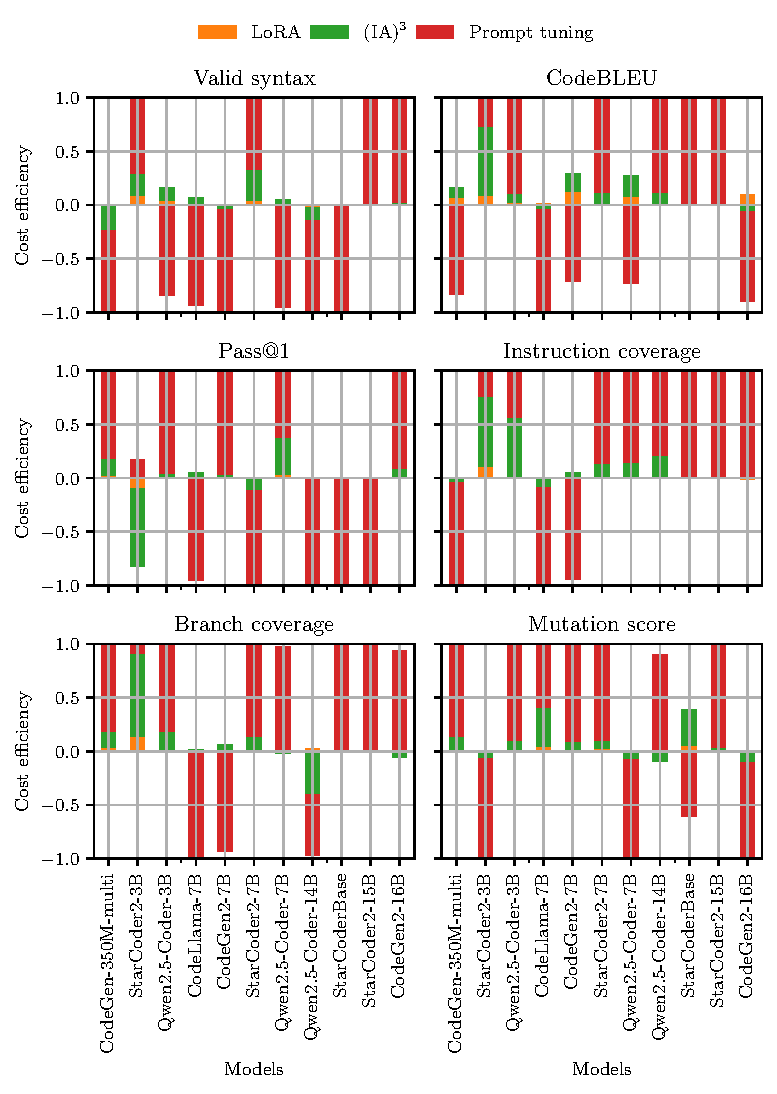
\includegraphics{figures/cost_efficiency.pdf}
    \caption{Stacked bar chart of symmetrically normalized metrics value differences (increase or decrease) between baseline and tuned models, divided by the percentage of trainable parameters of models, on the \textsc{Methods2Test\textsubscript{runnable}} dataset.}
    \label{fig:relative-importance}
\end{figure}

\Cref{fig:relative-importance} shows the results of the metrics (valid syntax, CodeBLEU, pass@1, instruction coverage, branch coverage, and mutation score) for each tuning method relative to the percentage of trainable parameters, symmetrically normalized between -1 and 1. As shown in \Cref{fig:relative-importance}, prompt tuning has the highest efficiency for every metric and is the method that you get the ``most bang for your buck.'' Moreover, prompt tuning has the most potential cost-effectiveness on models with large sizes, i.e., Qwen2.5-Coder-14B, StarCoderBase, StarCoder2-15B, and CodeGen2-16B. This can be explained by the increased capacity of larger models to better understand and leverage the additional context provided by prompt tuning. However, prompt tuning does not show consistent superiority for all the models. The method contributes to negative performance in three models (StarCoder2-3B, CodeLlama-7B, and CodeGen2-7B). 

For the four smallest models (Qwen2.5-Coder-3B, CodeGen-350M-multi, CodeGen2-1B, and StarCoder2-3B), (IA)\textsuperscript{3} clocks in at second place, which provides better results than LoRA. However, (IA)\textsuperscript{3} generally fails to efficiently improve the three largest models. LoRA achieves a relatively low efficiency compared to the other PEFT methods. However, with the exception of pass@1, it does not lead to any significant negative impact on the performance of any of the models. Full fine-tuning obviously has the worst efficiency, as it needs to train all the model parameters.

\vspace{1em}
\noindent\fbox{%
    \parbox{\columnwidth}{%
        \textbf{Summary for RQ2}: PEFT methods offer significantly reduced computational requirements compared to full fine-tuning and are ranked by resource utilization effectiveness as follows: prompt tuning $>$ (IA)\textsuperscript{3} $>$ LoRA $>$ full fine-tuning. Prompt tuning demonstrates the highest returns on investment for most models but also carries risks of negative performance impact. 
    }%
}

\section{Discussion}
\label{chap:discussion}
This section highlights our novel insights by comparing our results with related work. We also discuss possible threats to the validity of our study and how we mitigate them. 

\subsection{Comparison with related studies}
As the effectiveness of PEFT methods is task-dependent, our results provide novel insights into their performance in the context of unit test generation.  \citet{Ayupov2022ParameterEfficientFO} conclude that LoRA is less effective than full fine-tuning for code generation. We show contradictory results that LoRA could be as good as or even more effective than fine-tuning in unit test generation. \citet{weyssow2024exploring} explored generating code from natural language instructions and concluded that LoRA is the most effective among the PEFT methods they evaluated. Our results show that prompt tuning is the most effective in terms of cost and resource utilization in unit test generation, although LoRA provides better performance without considering the cost aspects. 

Compared to the existing studies, we also performed a more comprehensive evaluation, as we invested significant efforts to compare all PEFT methods to full fine-tuning across all model sizes (up to 16 billion parameters). In contrast, \citet{Ding2023ParameterefficientFO} only evaluated PEFT using the 355 million parameter RoBERTa\textsubscript{LARGE} model, while \citet{weyssow2024exploring} only did full fine-tuning for smaller models up to a maximum of 350 million parameters. While existing works on code generation or test generation have demonstrated promising results, they are often limited to artificially constructed benchmarks such as HumanEval. These datasets are typically small, synthetically curated, and lack the complexity of real-world software systems. As our results show, such controlled settings also overlook critical challenges that arise in real-world scenarios, such as missing dependencies, inconsistent, or erroneous code. Defects4J \citep{just2014defects4j}, one of the more realistic benchmarks available, contains only 17 repositories. This starkly contrasts the scale and messiness of actual industrial or open-source projects. As a result, prior work such as \citet{alagarsamy2024a3test} may significantly overestimate the robustness and generalizability of models when deployed beyond synthetic testbeds. Our evaluation, grounded in more realistic settings using \textsc{Methods2Test} \citep{tufano2021unit}, highlights these limitations and emphasizes the need for evaluation frameworks that reflect the true complexity of software development.

Several studies have leveraged LLMs for generating unit tests \citep{tufano2021unit, siddiq2024using, yuan2023manual, schäfer2023empirical, steenhoek2023reinforcement}. However, none of the works investigate the potential performance of using PEFT compared to full fine-tuning. \citet{tufano2021unit} automatically generated unit tests and reported 95\% syntactic correctness when training BART large (400 million parameters) \citep{lewis2019bart} on \textsc{Methods2Test}. With PEFT methods, we can generate an average median of 96\% syntactically correct unit tests. Training between 20 thousand and 13 million parameters on 1\% of the same data, showcasing the potentially powerful performance of PEFT methods.

Different from studies \citep{siddiq2024using, yuan2023manual, schäfer2023empirical} using large instruction-tuned enterprise LLMs such as ChatGPT to generate test cases, this study focused on generating test cases from autoregressive base code models. Compared to e.g. \citet{schäfer2023empirical}, our best model produced 13\% less statement coverage and 55\% lower branch coverage. Achieving state-of-the-art performance was not the focus of our work. Instead, our work provides an empirical evaluation of PEFT methods in a more practical scenario, where organizations can efficiently customize models for their own testing needs. One reason for the reduced coverage is probably due to the size differences of the models. The largest model we evaluated had 16 billion paramaters, opposed to the lager commercial GPT-3.5-Turbo. Our results shown in \Cref{tab:eval-summary} illustrate that larger models generally generate better unit tests than smaller ones. Another reason is probabaly due to the differences between the benchmark datasets used by our study. We use a real-world evaluation dataset that is more diverse, spanning 119 repositories, versus the 25 npm packages used by \citet{siddiq2024using}. Our analyses on the reasons for low pass@1 rates show that it is necessary to consider potential compilation and code dependency issues when using LLMs to generate executable unit tests, providing valuable novel insights to improve unit test generation using PEFT or ChatGPT. Opposed to related works like \citep{siddiq2024using, yuan2023manual, schäfer2023empirical}, we conduct mutation testing. As our results depict in \cref{sec:mutation-score}, measuring mutation score is crucial to ensure generated tests are actually able to reveal faults.

\subsection{Implications to Academia and Industry}
Writing unit tests is a hard and often time-consuming task \citep{7102609}. However, they are essential to ensure code quality, stability, and maintainability \citep{Gonzalez2017ALS}. Automating unit test generation using LLMs can significantly reduce the time and effort required for this process, making it an attractive solution for academia and industry. As our experiments show, full fine-tuning is sometimes required to achieve adequate quality of the generated unit tests, which is computationally demanding. Many LLM users may not have the necessary computing resources to fine-tune LLMs fully. Our results show that various PEFT methods can achieve similar performance to full fine-tuning by training a minuscule parameter fraction. Furthermore, our results suggest starting with prompt tuning for cost-effectiveness. Then, if stability issues arise, LoRA should be considered as a reliable alternative because it does not lead to a negative performance impact. 

\subsection{Threats to Validity}

\subsubsection{External validity}
One of the threats to external validity is the selection of models. We minimize this threat by selecting a broad range of models varying in size, pre-training data, and learning objectives. As we have have spent upward of 700 GPU hours for model tuning alone, exploring an even broader range of alternative models is constrained due to cost. Another potential concern is the validity of the benchmarking dataset. We chose to use \textsc{Methods2Test}, which is the largest publicly available corpus of real-world Java unit test cases and corresponding focal methods. We believe this provides a representative evaluation setting compared to existing studies like \citet{alagarsamy2024a3test}, although future work should expand the analysis to other programming languages to ensure generalizability. The last threat is related to our evaluation metric. While popularly used, we recognize BLEU as a sub-optimal performance estimator for code generation. We, therefore, employ a more code-friendly version, CodeBLEU. Although CodeBLEU may not be the optimal metric to evaluate the functional correctness of unit tests completely, it provides a good tradeoff between evaluation effort and validity. To supplement our evaluation, we have also spent significant effort developing evaluation pipelines, as well as over 200 CPU hours for executing the test in the \textsc{Methods2Test\textsubscript{runnable}} dataset, calculating pass@1, code coverage, and mutation scores.

\subsubsection{Internal validity}
The main threat to internal validity is comprised of the selection of hyperparameters. We use the hyperparameters reported in the introductory paper of each PEFT method to avoid introducing unnecessary biases. Additionally, we use greedy decoding to support reproducibility and reduce variability in the generated results.

\section{Conclusion and Future Work}
\label{chap:conclusion}
Although PEFT has been investigated to boost the quality and efficiency of code-related tasks using LLMs, they have not been studied in the context of unit test generation. We performed the first empirical study to compare different PEFT methods and full fine-tuning to generate unit tests. Our comparison involved thirteen LLMs of different sizes and architectures. Our results offer valuable insights into the advantages and challenges of using PEFT and full fine-tuning for unit test generation. With the knowledge we've gathered, individuals can choose the most suitable PEFT methods or full fine-tuning based on the size and characteristics of the LLMs. In future work, we plan to extend the analysis perform an empirical comparison of methods for tuning instruction-based LLMs, covering both PEFT methods per se and variations in prompt templates

In addition to unit tests, manually coding other automated test cases, such as integration and system tests, can be cost-intensive. In the future, we intend to explore the utilization of LLMs in conjunction with cost-effective tuning methods to automatically generate other types of tests.

\section*{Acknowledgements}
The empirical results were supported through the computational resources of HPC facilities at the Norwegian University of Science and Technology (NTNU) \citep{sjalander2019epic}.

\section*{Data Availability}
\noindent The \textsc{Methods2Test\textsubscript{small}} dataset is available at:\\
\url{https://huggingface.co/datasets/andstor/methods2test_small}\\

\noindent The \textsc{Methods2Test\textsubscript{runnable}} dataset is available at:\\
\url{https://huggingface.co/datasets/andstor/methods2test_runnable}\\

\noindent The \textsc{Methods2Test\textsubscript{meta}} dataset is available at:\\
\url{https://huggingface.co/datasets/andstor/methods2test_meta}\\

\noindent Metadata and links to the trained models can be found at:\\
\url{https://huggingface.co/datasets/andstor/peft-unit-test-generation-experiments}\\

\noindent Experiment code and results are available at:\\
\url{https://github.com/andstor/peft-unit-test-generation-replication-package}







\chapter{Discussion}
Lorem ipsum dolor sit amet.

\chapter{Conclusion}
Lorem ipsum dolor sit amet.



\subsection{Problem Statement}
In recent years, the field of language modeling has taken a huge leap in general language understanding. Large-scale transformer models \cite{vaswani2017attention} have shown great potential for general language understanding, surpassing almost every state-of-the-art language modeling task. This is especially due to the transformer's outstanding capability of transfer learning. Enormous amounts of resources are spent on pre-training transformer models on general knowledge. These models can then be fine-tuned for more specific tasks, building upon the already pre-trained knowledge.

Automatic code generation is by many considered the "holy grail" in the field of computer science \cite{PGL-010}. Recent works have applied transformers for code generation and program synthesis, achieving state-of-the-art results. For example, Codex by \textcite{chen2021codex} fine-tunes GPT-3 \cite{brown2020language} on code data from GitHub. Google DeepMind's AlphaCode by \textcite{li2022competition} trained an encoder-decoder model on code data from GitHub and fine-tuned it for competitive programming challenges.

Still, many challenges remain. One area of interest is the computational resources required for training the models. To update the model on new data, one often has to redo the entire fine-tuning process, an extremely resource-demanding process. Another problem is model bias. Due to the extensive data requirements for training these large models, the models often exhibit a lot of bias \cite{chen2021codex}. This could be everything from offensive language to vulnerable code.

The area of code synthesis with large language models is still in its early days. Especially interesting is the generation of smart contracts, which is the source code of blockchain applications. Although tricky to get right, smart contracts are often rather small and self-contained, making them a good candidate for automatic code generation. Some attempts have been made at summarizing smart contract code with large language models \cite{yang2021multimodal}. However, none have attempted the opposite, to automatically generate the smart contract code. This is what I have addressed in my master's thesis, in addition to investigating how to avoid introducing security vulnerabilities in the generated smart contract code. The doctoral thesis will be a continuation of my work, further investigating topics that would make the creation of smart contracts more available to people without expert knowledge, while simultaneously ensuring the generated code keeps high quality, is maintainable, and secure.

\subsection{Research Motivation}

However, besides bringing enhanced efficiencey, there is a lack of quality. The main motivation is to enable these automatic code generation systems to produce maintainable, secure, and correct code.


\begin{figure}[htbp]
    \centering
    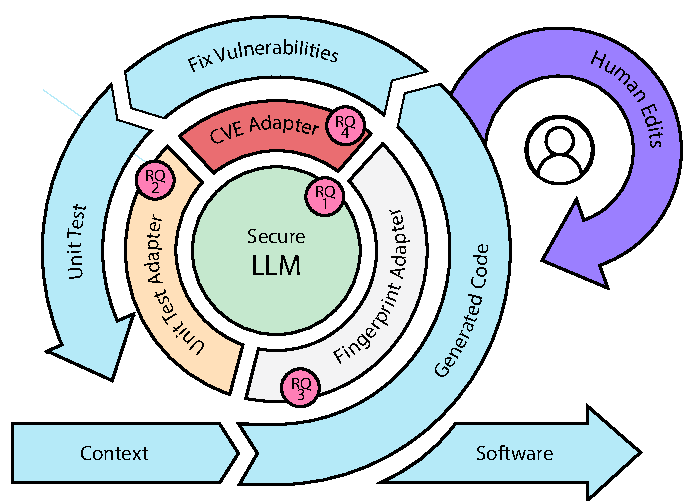
\includegraphics{figures/code_generation_lifecycle.pdf}
    \caption{Towards a holistic code generation framework.}
\end{figure}

\subsection{Research Questions}
The thesis aims to address the research motivations by answering the research questions for the thesis.

The overarching goal of the thesis is to figure out \textit{How to generate code that keeps high quality, is maintainable, and secure, using Large language models?}. This problem is broken down into five research questions. They are as follows:

\begin{enumerate}[leftmargin=2cm,label=\textbf{RQ\arabic*}:]
    \item How to automatically generate secure code with large language models?
    \item How to automatically generate unit tests?
    \item How to automatically generate integration tests?
    \item How to automatically fix code vulnerabilities introduced by humans?
\end{enumerate}


\begin{figure}[htbp]
    \centering
    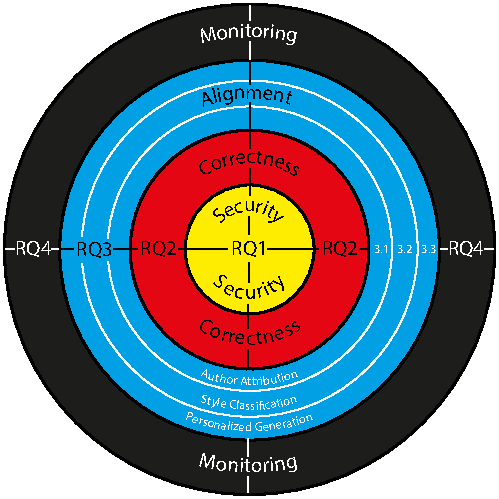
\includegraphics{figures/research_questions_bullseye.pdf}
    \caption{Research questions objectives and relation.}
\end{figure}

\subsection{Research Outcomes}


\subsubsection{Research Contributions}

\begin{enumerate}[leftmargin=2cm,label=\textbf{C\arabic*}:]
    \item \textit{New method for generating safe code with LLMs.} How to automatically generate secure code with large language models?
    \item \textit{New knowledge about how PEFT can be used for enhancing unit test generation.} How to automatically generate unit tests?
    \item \textit{New knowledge about how LLMs for code are able to adhere to the existing style.} How to align large language models with a developer's style, or ``fingerprint''.
    \item How to align large language models with a developer's style, or ``fingerprint''.
    \item How to automatically fix code vulnerabilities introduced by humans?
\end{enumerate}


\begin{table}[htp]
    \newcolumntype{Y}{>{\centering\arraybackslash}X}
    \centering
    \caption{Relationship between publications, research questions (RQs) and contributions.}
    \label{tab:my_label}
    
    \begin{tabularx}{\textwidth}{l|YYYY|YYYY}
        \toprule
         & \multicolumn{4}{c}{\textbf{Research Questions}} & \multicolumn{4}{c}{\textbf{Contributions}}\\
         \textbf{Papers} & RQ1 & RQ2 & RQ3 & RQ4 & C1 & C2 & C3 & C4\\
        \midrule
        Paper A - Vulnerability-constrained decoding & \bullet & & & & \bullet & & & \\
        Paper B - Unit Test Generation & & \bullet & & & & \bullet & & \\
        Paper C - Source Code Author Attribution & & & \bullet & & & & \bullet & \\
        Paper D - Can LLMs follow code style? & & & \bullet & & & & \bullet & \\
        Paper E - Aligning LLMs to code fingerprints & & & \bullet & & & & \bullet & \\
        Paper F - Automatic fixing of code vulnerabilities & & & & \bullet & & & & \bullet\\
        \bottomrule
    \end{tabularx}
\end{table}

\begin{table}[htp]
    \newcolumntype{Y}{>{\centering\arraybackslash}X}
    \centering
    \small
    \caption{Dissemenation Plan}
    \label{tab:my_label}
    
    \begin{tabularx}{\textwidth}{cp{5cm}XlXX}
        \toprule
        \textbf{ID} & \textbf{Title} & \textbf{Publisher} & \textbf{Conference} & \textbf{Method} & \textbf{Status} \\
        \midrule
        A & Efficient Avoidance of Vulnerabilities in Auto-completed Smart Contract Code Using Vulnerability-constrained Decoding & IEEE & ISSRE 2023 \cite{issre} & Design Science \cite{ralph2021empirical} & Published \\
        B & Parameter-Efficient Fine-Tuning of Large Language Models for
Unit Test Generation: An Empirical Study & IEEE/ACM & ASE 2024 \cite{ase} & Benchmarking \cite{ralph2021empirical} & Submitted \\
        C & Source Code Authorship Attribution Using Large Language Models & IEEE/ACM & ICSE 2025 \cite{icse} & Design Science \cite{ralph2021empirical} &  \\
        D & Can LLMs follow code style? & ??? & ??? \cite{icse} &   Exploratory Data Science \cite{ralph2021empirical}& ??? \\
        E & Aligning LLMs to code fingerprints & ??? & ??? & ???\\
        F & Automatic fixing of code vulnerabilities & ??? & ??? & ???\\
        \bottomrule
    \end{tabularx}
\end{table}

contrib
new method for generating secure code

Knowledge on test generation peft


We propose a novel vulnerability-constrained decoding approach to avoid vulnerabilities in the generated code efficiently and effectively. The approach can help com- panies quickly update LLMs to avoid the negative con- sequence caused by vulnerabilities in the model training dataset.

We conducted the first empirical study to extensively eval-
uate training LLMs using various PEFT methods—LoRA,
(IA)3, and prompt tuning—for unit test generation across a
wide range of LLM models

\subsection{Paper A - Secure code generation}

\textbf{Efficient Avoidance of Vulnerabilities in Auto-completed Smart Contract Code Using Vulnerability-constrained Decoding}\\\\
\noindent Andr\'e Storhaug, Jingyue Li, Tianyuan Hu\\\\
\noindent \textbf{Published in}: 2023 IEEE 34th International Symposium on Software Reliability Engineering (ISSRE), Florence, Italy, 2023, pp. 683-693, doi: 10.1109/ISSRE59848.2023.00035.\\\\
\noindent \textbf{Research Question}: RQ1\\\\
\noindent \textbf{Main Area of Contribution}: \\\\

Masters use only $$<|secure|> and <|vulnerable|>$$ labels. Vulnerability constrained decoding builds upon initial work done in master thesis. the approach is refined and greatly improved. Uses actually vulnerability types. Named vulnerability constraned decoding.

For my master thesis, I have studied how to automatically generate secure smart contract code for the Ethereum blockchain. The code generation was done by fine-tuning a 6-billion parameter large transformer model (GPT-J \cite{gpt-j}) on a smart contract dataset consisting of 53 million lines of code. Contributions include the currently largest smart contract dataset, and a state-of-the-art automatic smart contract code generation model. In addition, the project tackles the problem of dataset bias, focusing on reducing security vulnerabilities that are introduced by these large-scale datasets. Using the code generator developed in my thesis, smart contract code developers can generate secure smart contract code by only writing comments to describe the functions to be provided by the code. The results and findings from my master thesis can be further analyzed and the approach refined in my PhD studies.

\subsection{Paper B - Unit Test Generation using PEFT}
\textbf{Parameter-Efficient Fine-Tuning of Large Language Models for Unit Test Generation: An Empirical Study}\\\\
\noindent Andr\'e Storhaug, Jingyue Li\\\\
\noindent \textbf{Research Question}: RQ2\\\\
\noindent \textbf{Main Area of Contribution}: \\\\

How to efficiently update the AI-model for providing up-to-date high-quality code?
Software development is an ever-evolving industry. Code libraries are updated, new vulnerabilities are discovered, APIs are changed, etc. As a developer, one of the primary skills is to be able to quickly adapt to such changes. For automatic code generation systems to be on par with humans, these systems must be also able to produce up-to-date high-quality code. However, training large transformer models normally entails an extremely high resource consumption. Investigating methods for efficient retraining and adaptations are therefore highly relevant. For example, in the area of smart contracts, a vast number of contracts are made available each day. By additively continuing training of large-scale transformer models in an energy-efficient way, one could ensure the model provides up-to-date high-quality code.

\subsection{Paper C - Source Code Author Attribution}

\textbf{Source Code Authorship Attribution Using Large Language Models}\\\\
\noindent Andr\'e Storhaug, Jingyue Li\\\\
\noindent \textbf{Research Question}: RQ3.1\\\\
\noindent \textbf{Main Area of Contribution}: \\\\

Another problem rooted in model bias is the issue of producing maintainable code. Due to the share volume of data needed for training large-scale transformer models, freely available code hosted on platforms such as GitHub is normally used for pre-training. A lot of the data available on such platforms are not maintainable, contains ad hoc solutions and has a bad coding style. This will inevitably affect the quality of the model's generated code. For automatic code generation to be used in a production setting, the generated code needs to be maintainable and understandable so that developers can integrate the manually developed code and the auto-generated code. Investigating methods for combating code smells, would massively improve the usefulness of such an automated system.

\subsection{Paper D - Code Style Classification}

\textbf{Can LLMs follow code style?}\\\\
\noindent Andr\'e Storhaug, Jingyue Li\\\\
\noindent \textbf{Research Question}: RQ3.2\\\\
\noindent \textbf{Main Area of Contribution}: \\\\

Another problem rooted in model bias is the issue of producing maintainable code. Due to the share volume of data needed for training large-scale transformer models, freely available code hosted on platforms such as GitHub is normally used for pre-training. A lot of the data available on such platforms are not maintainable, contains ad hoc solutions and has a bad coding style. This will inevitably affect the quality of the model's generated code. For automatic code generation to be used in a production setting, the generated code needs to be maintainable and understandable so that developers can integrate the manually developed code and the auto-generated code. Investigating methods for combating code smells, would massively improve the usefulness of such an automated system.



\subsection{Paper D - Personalized Code Generation?}

\textbf{Aligning LLMs to code fingerprints}\\\\
\noindent Andr\'e Storhaug, Jingyue Li\\\\
\noindent \textbf{Research Question}: RQ3.3\\\\
\noindent \textbf{Main Area of Contribution}: \\\\

Automatic code generation could help developers produce more secure, maintainable, and high-quality code at a fast pace. By further combining graphical tools like VPL \footnote{Microsoft Visual Programming Language (VPL) \url{https://docs.microsoft.com/en-us/previous-versions/microsoft-robotics/bb483088(v=msdn.10)}} with automatic code generation, one could extend a lot of these benefits to users beyond the standard developer.  No-code solutions are increasing in popularity, however, most of these systems are still rooted in standard code generation techniques. By leveraging the capabilities of large-scale language models, one could significantly enhance and simplify how the user interacts with such systems. It could open up new and more flexible ways for how programs are created. Not only would this greatly lower the threshold for non-developers to leverage programming, but also increased efficiency due to a simpler developing process.


\subsection{Paper E - Security fixing?}

\textbf{Automatic fixing of code vulnerabilities}\\\\
\noindent Andr\'e Storhaug, Jingyue Li, Jiamou Sun, Jieshan Chen, Zhenchang Xing\\\\
\noindent \textbf{Research Question}: RQ3.3\\\\
\noindent \textbf{Main Area of Contribution}: \\\\



\section{Academic Training}

\subsection{Plan for Completion}
\lipsum[1-2]
\begin{figure}[htpb]
%\thispagestyle{empty}
%\begin{landscape}
	\clearpage
	%\newgeometry{margin=2.5cm, top=20mm, bottom=35mm}
\definecolor{foobarblue}{RGB}{0,153,255}

\newganttchartelement{mainbar}{
    mainbar/.style={
        draw=foobarblue!10!black,
        fill=foobarblue!10
    },
    mainbar label font=\bfseries
}

\newganttlinktype{f-m}{
 \ganttsetstartanchor{on right=1}
 \ganttsetendanchor{on left=0}
 \draw[/pgfgantt/link]
  ([xshift=-.2pt]\xLeft, \yUpper) -- 
  (\xRight, \yLower);
}

\hspace{-2cm}
\noindent
\begin{ganttchart}[
    progress=today,
    today=25,
    today label=August,
    hgrid,
    vgrid={*{2}{draw=none},{dotted}},
    vrule label font=\tiny,         
    title label font=\tiny,
    %bar label font=\tiny,
    %milestone label font=\tiny,
    %group label font=\bfseries\small,
    bar height = 0.4,
    %milestone left shift =-1,
    %milestone right shift =1,
    x unit=0.325cm,
    y unit title=.6cm,
    %y unit chart=0.85cm,
    y unit chart=0.7cm,
    link bulge = 2,
    bar label node/.append style={align=left},
    link/.style={-latex, draw=red, fill=red, thick}
    ]{1}{42}
    %labels
    \gantttitle[]{2022}{6}                 % title 2
    \gantttitle[]{2023}{12}
    \gantttitle[]{2024}{12}
    \gantttitle[]{2025}{12}\\
    \gantttitlelist{"Q3","Q4"}{3}
    \gantttitlelist{"Q1","Q2","Q3","Q4"}{3}
    \gantttitlelist{"Q1","Q2","Q3","Q4"}{3}
    \gantttitlelist{"Q1","Q2","Q3","Q4"}{3}\\
    %tasks
    \ganttgroup{Organised academic training}{2}{30} \\
    \ganttbar{Corse IDT8000}{2}{6} \\
    \ganttbar{Corse IDT80002}{2}{6} \\
    \ganttbar{Corse DT8111}{7}{12} \\
    \ganttbar{Corse DT8806}{7}{12} \\
    \ganttbar{FYS-8805 (Winter school)}{7}{7} \\
    \ganttbar{Corse DT8114}{25}{30} \\
    
    \ganttgroup{Research}{2}{34} \\
    \ganttset{ bar/.append style={fill=yellow}, bar incomplete/.append style={fill=yellow!10}}%
    \ganttbar[name=RQ1]{RQ1}{2}{12} \\
    \ganttmilestone[name=M1]{Paper to ISSRE 2023}{12} \\
    \ganttset{ bar/.append style={fill=red}, bar incomplete/.append style={fill=red!10}}%
    \ganttbar[name=RQ2]{RQ2}{13}{24} \\
    \ganttmilestone[name=M2]{Paper to ASE 2024}{24} \\
    %\ganttbar[name=RQ3]{RQ3}{24}{25} \\%6+12+7 /juni
    \ganttset{ bar/.append style={fill=blue}, bar incomplete/.append style={fill=blue!10}}%
    \ganttbar[name=RQ31]{RQ3.1}{24}{26}\\ %6+12+7 /juni
    \ganttmilestone[name=M31, milestone label node/.append style={align=right}]{Paper to ICSE 2025}{26}\\
    \ganttbar[name=RQ32]{RQ3.2}{27}{28} \\
    \ganttmilestone[name=M32, milestone label node/.append style={align=right}]{Paper to JSS 2025}{28}\\
    \ganttbar[name=RQ33]{RQ3.3}{29}{34} \\
    \ganttmilestone[name=M33, milestone label node/.append style={align=right}]{Paper to TSE 2025}{34}\\
    %\ganttmilestone{}{29}
    %\ganttmilestone{}{25}\\
    \ganttgroup[group label node/.append style={align=right}]{Exchange to CSIRO's Data61}{27}{32}\\
    \ganttset{ bar/.append style={fill=black}, bar incomplete/.append style={fill=black!50}}%
    \ganttbar[name=RQ4]{RQ4}{27}{32} \\
    \ganttmilestone[name=M4]{Paper to ?}{32} \\
    \ganttbar[name=T1]{\textbf{Thesis writing}}{35}{39} \\
    \ganttmilestone[name=W1, milestone label node/.append style={align=right}]{Deliver thesis}{39}
    % 
    \ganttlink[link type=f-m]{RQ1}{M1}
    \ganttlink[link type=f-m]{RQ2}{M2}
    \ganttlink[link type=f-m]{RQ31}{M31}
    \ganttlink[link type=f-m]{M31}{RQ32}
    \ganttlink[link type=f-m]{RQ32}{M32}
    \ganttlink[link type=f-m]{M32}{RQ33}
    \ganttlink[link type=f-m]{RQ33}{M33}
    \ganttlink[link type=f-m]{RQ4}{M4}
    \ganttlink[link type=f-m]{T1}{W1}
    %\ganttlink{RQ2}{RQ3}
    %\ganttlink{RQ3}{RQ4}
    %\ganttlink{RQ4}{W1}
\end{ganttchart}
%\restoregeometry
	\caption{Gantt diagram of working plan.}
	\label{fig:gantt-diagram-progress-plan}
\end{figure}


\subsection{Changes in Academic Content}


\subsection{Organised Academic Training}


\begin{table}[htp]
    \newcommand\T{\rule{0pt}{2.6ex}}       % Top strut
    \newcommand\B{\rule[-1.2ex]{0pt}{0pt}} % Bottom strut
    \centering
    \caption{Course plan status}
    \label{tab:my_label}
    
    \begin{tabularx}{\textwidth}{Xllcc}
        \toprule
        \textbf{Code} & \textbf{Title} & \textbf{Term} & \textbf{Level} & \textbf{ECTS}\\
        \midrule
        \multicolumn{5}{l}{\cellcolor{green!20}{\textbf{Completed}}} \bigstrut\\
        \T IDT8000 & Research Ethics & 2022 A & PhD & 2.5\\
        IDT8002 & Project development and management & 2022 A & PhD & 2.5\\
        DT8111 & Empirical research methodologies in ID and digitalization & 2023 S & PhD & 7.5\\
        DT8806 & ISSE Research Topics and Academic Writing & 2024 S & PhD & 7.5\\
        FYS-8805 & NLDL Deep Learning Winter School 2023 & 2023 S & PhD & 5\\
        \midrule
        \multicolumn{4}{l}{Total completed ETCS} & 25\\
        \midrule
        \midrule
        \multicolumn{5}{l}{\cellcolor{yellow!20}{\textbf{Planned}}} \bigstrut\\
        \T DT8114 & PhD Seminar in Computer and Information Science & 2023 S & PhD & 7.5\\
        \midrule
        \multicolumn{4}{l}{Total planned ETCS} & 7.5\\
        \midrule
        \bottomrule
    \end{tabularx}
\end{table}


\subsection{Academic services}

Every other week?

"Co-supervised" find name of previous student.
Co-supervisor for Petter Dahlen master thesis.

Web Co-host together with Alicia for FSE 2025.

\subsection{Community Engagement}

\begin{table}[htp]
    \newcommand\T{\rule{0pt}{2.6ex}}       % Top strut
    \newcommand\B{\rule[-1.2ex]{0pt}{0pt}} % Bottom strut
    \centering
    \caption{Course plan status}
    \label{tab:my_label}
    
    \begin{tabularx}{\textwidth}{lllXc}
        \toprule
        \textbf{Code} & \textbf{Title} & \textbf{Term} & \textbf{Level} & \textbf{ECTS}\\
        \midrule
        \multicolumn{5}{l}{\cellcolor{green!20}{\textbf{Completed}}} \bigstrut\\
        \T IDT8000 & Research Ethics & 2022 A & PhD & 2.5\\
        IDT8002 & Project development and management & 2022 A & PhD & 2.5\\
        
    \end{tabularx}
\end{table}

Winterschool Tromsø


NORAI conference

Workshop birgit (sustainability?)
ISSE seminar
Intensive course on scientific publishing
Blockheim 2024 - Trondheim Open Blockchain Meetup
Attended ICSE conference


\subsection{External Research Stay}



\section{Ethical reflections}
The very nature of machine learning models gives raise to several ethical issues. Firstly, these systems might be biased. If the dataset used for training is biased, the model might perpetuate social prejudices and injustices. Proper care should be taken to reduce the likelihood of producing biased models. Secondly, the systems might be used for evil. Automatic code generation can significantly increase productivity of developers. However, these systems may also help attackers write malicious code. It is therefore important to thoroughly assess these capabilities before releasing models to the general public, ensuring that the benefits outweigh the risks.

\section{Sustainability}
One of the more important UN goal is the 13th: climate action. Global warming is one of the most critical challenges the world is facing today. Large-scale transformer model requires a huge amount of training resources. Of special significance is the amount of electricity required to power the necessary computing platform. For example, the estimated carbon emissions due to training GPT-3, a 175 billion parameter transformer model, are 552 tonnes $CO_2$ and an energy consumption of 1287 MWh \cite{patterson2021carbon}. In my research, I will primarily aim to reuse (fine-tune) existing models, keeping both the environmental impact and costs as low as possible. Further, by making most of the results from this research open source, others may benefit from this work. By making both models and datasets available for other researchers and the general public, this will reduce the need for everyone creating their own solution, further reducing the required climate footprint. This is also naturally related to the 12th UN goal: responsible consumption and production. In relation to the ethical aspects of bias described in the previous section, this concerns both the 5th and 10th UN sustainability goals; Gender equality and Reduced inequalities.

\section{Conclusion}


%\bibliographystyle{ieee}
\vspace{1cm}
\newpage
\printbibliography
\end{document}



//. some comment
function helloworld(int number) retunr {

    print(98ifi
    }
    
    /comment
    
    
    
// print hello 
